\documentclass{report}
\usepackage[utf8]{inputenc}    
\usepackage[T1]{fontenc}
\usepackage[francais]{babel}
\usepackage{wrapfig}
\usepackage{graphicx}
\usepackage{xcolor}
\usepackage{appendix}
\usepackage{adjustbox}
\usepackage{titling}
\usepackage{float}
\usepackage{pdfpages}
\usepackage{caption}
\usepackage{subcaption}
\usepackage{arydshln}
\usepackage{fixltx2e}
\usepackage{amsmath}
\usepackage{pdflscape}


% Rotation de texte
\newcommand*\rot{\rotatebox{90}}

\newcommand*\halfrot{\rotatebox{135}}

% Alias pour texte en indice
\newcommand{\indice}{\textsubscript}

% Vecteur colonne
\newcommand{\colvect}[1]{\ensuremath{\begin{pmatrix}#1\end{pmatrix}}}



%Géométrie des pages
\usepackage{geometry}
\geometry{hmargin=2.2cm,vmargin=2.2cm}


%Profondeur des compteurs et de la tableofcontents
\setcounter{secnumdepth}{3}
\setcounter{tocdepth}{3}



\addto\captionsfrench{%
  \renewcommand\appendixname{Annexe}
  \renewcommand\appendixpagename{Annexes}
}



\begin{document}

\begin{titlepage}
	\centering
	
    \vspace*{1.2 cm}
    
   	\textsc{\LARGE Master i informatique\\Travail Encadré de Recherche\\[0.3cm]\large Juin 2018}

	\vspace{2.2cm}
    
    
	\rule{\linewidth }{0.2 mm} \\[0.15 cm]
    {\LARGE \textbf{Rapport QuChemPedia}\\[0.2cm] \large
		\textbf{Sous titre}}\\
	\rule{\linewidth}{0.2 mm}
       \vspace*{0.1 cm}
	
	\begin{center}
	\vspace{0.3cm}
	
	\emph{Auteur}\\
	\vspace{0.1cm}
	Jules \bsc{Leguy}\\ 
	
	
	\vspace{0.5cm}
	\emph{Encadrants}\\
	\vspace{0.1cm}
	Benoit \bsc{Da Mota}\\
	Thomas \bsc{Cauchy}
	\end{center}		
	
	\vspace{1.0cm}


    
    
\end{titlepage}


\tableofcontents

\chapter{Introduction}
	\subsection{Motivation}

Les modèles décrits dans ce chapitre ont pour objectif de prédire la longueur de liaison optimisée entre des atomes partageant une liaison covalente au sein d'une molécule. L'objectif n'est donc pas de résoudre le problème de prédiction d'une géométrie moléculaire convergée complète, mais plutôt d'en résoudre une version locale simplifiée. Chronologiquement, cette classe de modèles est apparue après l'abandon des modèles tentant de prédire la géométrie optimisée complète d'une molécule (REF ABANDON DELTA\_DIST).\\
Puisque l'on résout le problème d'optimisation géométrique entre des couples d'atomes, la question de la façon d'utiliser cette méthode pour optimiser la géométrie complète d'une molécule se pose, nous n'y apportons cependant pas de réponse dans ce chapitre. L'objectif de ces modèles est en effet avant tout de valider notre capacité à effectuer des prédictions d'ordre géométrique de précision suffisante sur certains types de liaisons (REF GENERALISATION). L'élaboration d'une méthode d'optimisation géométrique moléculaire complète basée sur la résolution de sous-problèmes locaux est un problème très complexe, qui fait partie des nouveaux objectifs du projet QuChemPedia (REF PERSPECTIVES MODULES).\\
\par De plus, nous utilisons en entrée des modèles décrits dans ce chapitre des données « parfaites », c'est à dire qu'elles représentent des géométries déjà convergées. Ces données d'entrée ne correspondent donc pas aux données qui seraient utilisées dans un cas d'utilisation réel. L'utilisation de ces données permet cependant d'évaluer la capacité de nos modèles à effectuer des prédictions géométriques lorsque les conditions sont favorables, ce qui représente une première étape dans l'élaboration d'un système permettant de prédire les géométries convergées complètes (REF PERSPECTIVES MODULES).

\subsection{Représentation des données}

\subsubsection{Données en entrée des modèles}
\par Les modèles décrits dans ce chapitre utilisent en entrée la représentation géométrique locale des liaisons covalentes (REF GEOM LOCALE), qui permet de représenter les atomes au voisinage d'une liaison. En plus des informations géométriques, on représente la masse et le numéro atomique de chaque atome au voisinage de la liaison. Le numéro atomique est encodé en \emph{one-hot encoding}, c'est à dire de façon booléenne. La discrétisation des numéros atomiques a pour but de ne pas instaurer de relation d'ordre entre les différents atomes et donc a priori de mieux guider les modèles lors de l'apprentissage. Elle implique toutefois qu'il faut déterminer une limite aux numéros atomiques des atomes acceptés par un modèle. En effet, cet encodage coûte un attribut pour chaque numéro atomique accepté, pour chaque atome au voisinage de la liaison. Afin de travailler sur des modèles de taille raisonnable, ils acceptent les atomes de numéros atomiques inférieurs ou égaux à celui du fluor, ce qui correspond à neuf attributs encodant le numéro atomique pour chaque atome du voisinage.
\par De même la classe positionnelle (REF CLASSE POS) de chaque atome par rapport à la liaison est représenté en \emph{one-hot encoding}, afin de ne pas représenter cette information sur un ensemble possédant une relation d'ordre.\\

\par Le tableau suivant présente le nombre d'attributs utilisés pour représenter chaque atome au voisinage d'une liaison.

\begin{figure}[!h]
	\centering
	
	\begin{tabular}{|c|c|c|c|c|}
		\hline
		\textbf{Classe positionnelle} & \textbf{Distances} & \textbf{Masse atomique} & \textbf{Numéro atomique} & \textbf{Total}\\ \hline
		3 & 2 & 1 & 9 & 15\\ \hline
	\end{tabular}
	\caption{Quantité d'attributs représentant chaque atome au voisinage d'une liaison}
\end{figure}

\subsubsection{Homogénéisation de la taille des entrées}
\par Les molécules possédant un nombre variable d'atomes et l'entrée des modèles étant de taille fixe, nous effectuons une procédure de \emph{padding}\footnote{Rembourrage} des données. Cela signifie que l'entrée des modèles est découpée en blocs, représentant chacun un atome au voisinage de la liaison. La taille des blocs dépend des attributs représentant chaque atome, et le nombre de blocs définit le nombre maximal d'atomes au voisinage des liaisons que les modèles peuvent traiter. Nous déduisons cette information de la taille des molécules que l'on choisit d'accepter en entrée des modèles. La grande majorité des molécules étant de taille inférieure à 60 (VOIR DONNEES DISTRIB TAILLES) et les deux atomes composant la liaison n'apparaissant pas dans les entrées, nous choisissons de limiter le voisinage de la liaison à 58 atomes.\\
\par La représentation d'une liaison en entrée des modèles est donc composée de 58 blocs de 15 attributs, soit 870 valeurs. Lorsqu'une liaison possède moins de 58 voisins, les blocs correspondant aux atomes non définis valent zéro.

\subsubsection{Représentation d'une liaison en entrée d'un modèle}

\par Nous détaillons la représentation en entrée d'un modèle prédictif de la liaison imaginaire utilisée comme exemple en (REF REPR LOCALE). On considère que l'atome a$_3$ est un atome d'azote et que l'atome a$_4$ est un atome d'oxygène.

\vspace{0.5cm}

\begin{figure}[!h]
	\centering
	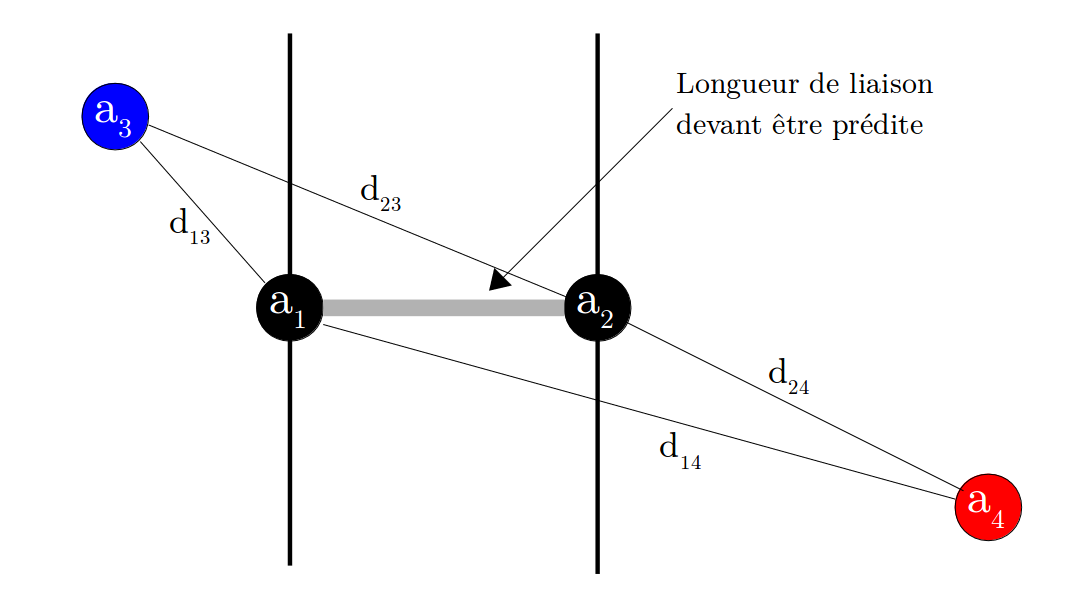
\includegraphics[scale=0.3]{images/classes_pos_4.png}
	\caption{Représentation schématique d'une liaison imaginaire}
\end{figure}

\par L'entrée correspondant à la liaison représentée ci-dessus est donnée dans le tableau suivant.

\begin{figure}[!h]
	\centering


	\begin{tabular}{|c|c|c|c|c|c|c|c|c|c|c|c|c|c|c|}
		\hline
		\multicolumn{3}{|c|}{\textbf{Classe pos.}} & \multicolumn{2}{|c|}{\textbf{Distances}} & \textbf{Masse atomique} & \multicolumn{9}{|c|}{\textbf{Numéro atomique}} \\
		\textbf{g?} & \textbf{c?} & \textbf{d?} & \multicolumn{2}{|c|}{}& & \textbf{H?} & \textbf{He?} & \textbf{Li?} & \textbf{Be?} & \textbf{B? }& \textbf{C?} & \textbf{N?} & \textbf{O?} & \textbf{F?} \\ \hline
		1 & 0 & 0 & $d_{13}$ & $d_{23}$ & 14,007 & 0 & 0 & 0 & 0 & 0 & 0 & 1 & 0 & 0 \\ \hline
		0 & 0 & 1 & $d_{14}$ & $d_{24}$ & 15,999 & 0 & 0 & 0 & 0 & 0 & 0 & 0 & 1 & 0 \\ \hline
		0 & 0 & 0 & 0 & 0 & 0 & 0 & 0 & 0 & 0 & 0 & 0 & 0 & 0 & 0 \\ \hline
		\rot{... } & \rot{... } & \rot{... } & \rot{... } & \rot{... } & \rot{... } & \rot{... } & \rot{... } & \rot{... } & \rot{... } & \rot{... } & \rot{... } & \rot{... } & \rot{... } & \rot{... }  \\ \hline 
		0 & 0 & 0 & 0 & 0 & 0 & 0 & 0 & 0 & 0 & 0 & 0 & 0 & 0 & 0 \\ \hline
	\end{tabular}

	\caption{Représentation des données d'une liaison en entrée d'un modèle prédictif}
\end{figure}



\subsection{Méthodologie}

\subsubsection{Précision requise}
\par Les modèles décrits dans ce chapitre travaillent sur des données « parfaites », c'est à dire qu'il prédisent des longueurs de liaisons dans des molécules dont la géométrie a déjà été optimisée. Cela nous permet de confirmer notre capacité à effectuer des prédictions d'ordre géométrique, mais pas de nous assurer que les modèles pourront effectuer de bonnes prédictions sur des données non optimisées issues de mesures ou de résultats théoriques. L'entraînement de modèles travaillant sur des données imparfaites fera l'objet de la suite du projet QuChemPedia (REF PERSPECTIVES). Pour pouvoir espérer obtenir de bonnes prédictions sur des données non optimisées, il faut obtenir de très bons résultats sur des données optimisées, comme on le montre en REF GENERALISATION.

\par La précision que l'on peut espérer atteindre avec les données sur lesquelles les modèles s'entraînent (REF PUBCHEM) est de l'ordre du picomètre (pm), soit $10^{-12}$ m. Cette précision dépend des fonctions choisies lors de l'optimisation géométrique quantique des molécules (REF OPTI DFT). Les modèles effectuant des prédictions dont l'erreur est inférieure à 1 pm confirmeront donc notre capacité à effectuer des prédictions d'ordre géométrique de précision suffisante.

\subsubsection{Classes de modèles}
\par Nous tentons de prédire les longueurs de liaisons entre plusieurs couples d'atomes, en entraînant un modèle par couple d'atomes formant une liaison. Les liaisons carbone-carbone ne seront alors pas prédites par le même modèle que les liaisons carbone-hydrogène. Cette séparation en sous-problèmes segmentés a pour objectif d'évaluer la précision que peuvent atteindre les modèles sur les problèmes les plus simples que l'on peut leur donner. L'évaluation de leur précision sur des problèmes plus complexes fait partie des futurs objectifs (REF	MODULES PLUSIEURS LIAISONS). La prédiction des longueurs de liaisons d'un unique couple donné d'atomes par modèle n'en fait toutefois pas un problème trivial, car elles peuvent sensiblement varier en fonction des atomes impliqués (REF DISTRIB LONGUEURS). Si les liaisons oxygène-hydrogène ont une taille variant en général entre 97 pm et 102 pm soit avec une amplitude de 5 pm, la taille des liaisons carbone-carbone varie entre 120 pm et 160 pm, ce qui représente une amplitude de 40 pm. \\
\par L'entraînement des modèles est un processus qui prend un temps non négligeable (REF CONTRAINTES MATERIELLES). Pour cette raison, nous n'entraînons pas tous les modèles sur un grand nombre d'exemples et nous définissons deux classes de modèles ayant des objectifs différents. \\
\par La première classe de modèles a un objectif d'expérimentation. Les modèles sont entraînés sur un nombre relativement faible d'exemples différents sur 150 époques (REF DEF EPOCH), ce qui représente environ 2h de préparation de données et 6h d'entraînement avec le matériel disponible. Ces modèles sont entraînés dans le but d'expérimenter de nouveaux traitements des données d'entrée ou de nouveaux paramètres. Ils ont pour objectif de discriminer la qualité de ces entrées et paramètres, c'est pourquoi ils travaillent sur la prédiction difficile des distances de liaisons carbone-carbone. Ces modèles sont décrits en REF PRED C.	\\
\par La seconde classe de modèles a un objectif de validation des paramètres performants issus de l'entraînement des modèles de la première classe, ainsi qu'un objectif de généralisation des méthodes à différents types de liaisons. Ces modèles s'entraînent donc sur plus d'exemples et sur plusieurs liaisons différentes (carbone-carbone, carbone-hydrogène et oxygène-hydrogène). L'entraînement des trois modèles de cette classe pour un ensemble d'entrées et de paramètres donné prend environ deux jours. Ces modèles sont décrits en REF GENERALISATION.

\subsection{Nomenclature}
\par Afin d'y faire référence simplement, nous nommons les différents modèles que l'on entraîne. Tous les modèles décrits dans ce chapitre ont pour préfixe \emph{DIST\_REL}, issu de leur vocation à prédire la distance relative entre les atomes d'une liaison, et pour suffixe le numéro chronologique de leur entraînement au sein de leur classe.\\
Les modèles de la première classe (resp. seconde) ont pour préfixe \emph{DIST\_REL\_C} (resp. \emph{DIST\_REL\_XY}, où X et Y désignent les symboles des éléments formant la liaison prédite). La différence de nomenclature entre les deux classes et notamment entre les modèles \emph{DIST\_REL\_C} et \emph{DIST\_REL\_CC} est discutable, mais a pour avantage de faire apparaître simplement la distinction.\\
Enfin, les modèles prédictifs n'étant pas des réseaux de neurones artificiels font apparaître leur type dans leur nom.


\chapter{Contexte et objectifs}
	\section{Projet QuChemPedia}
		\label{quchempedia}

\par Ce travail s'inscrit dans le cadre du projet QuChemPedia\footnote{Quantum Chemistry Encyclopedia}. Il s'agit d'un projet de recherche mené à l'initiative de Thomas Cauchy et Benoit Da Mota, respectivement chercheurs à MOLTECH Anjou (laboratoire de recherche en chimie) et au LERIA (laboratoire de recherche en informatique). Ces deux laboratoires sont situés à la faculté des sciences d'Angers.\\

\begin{figure}
	\centering
	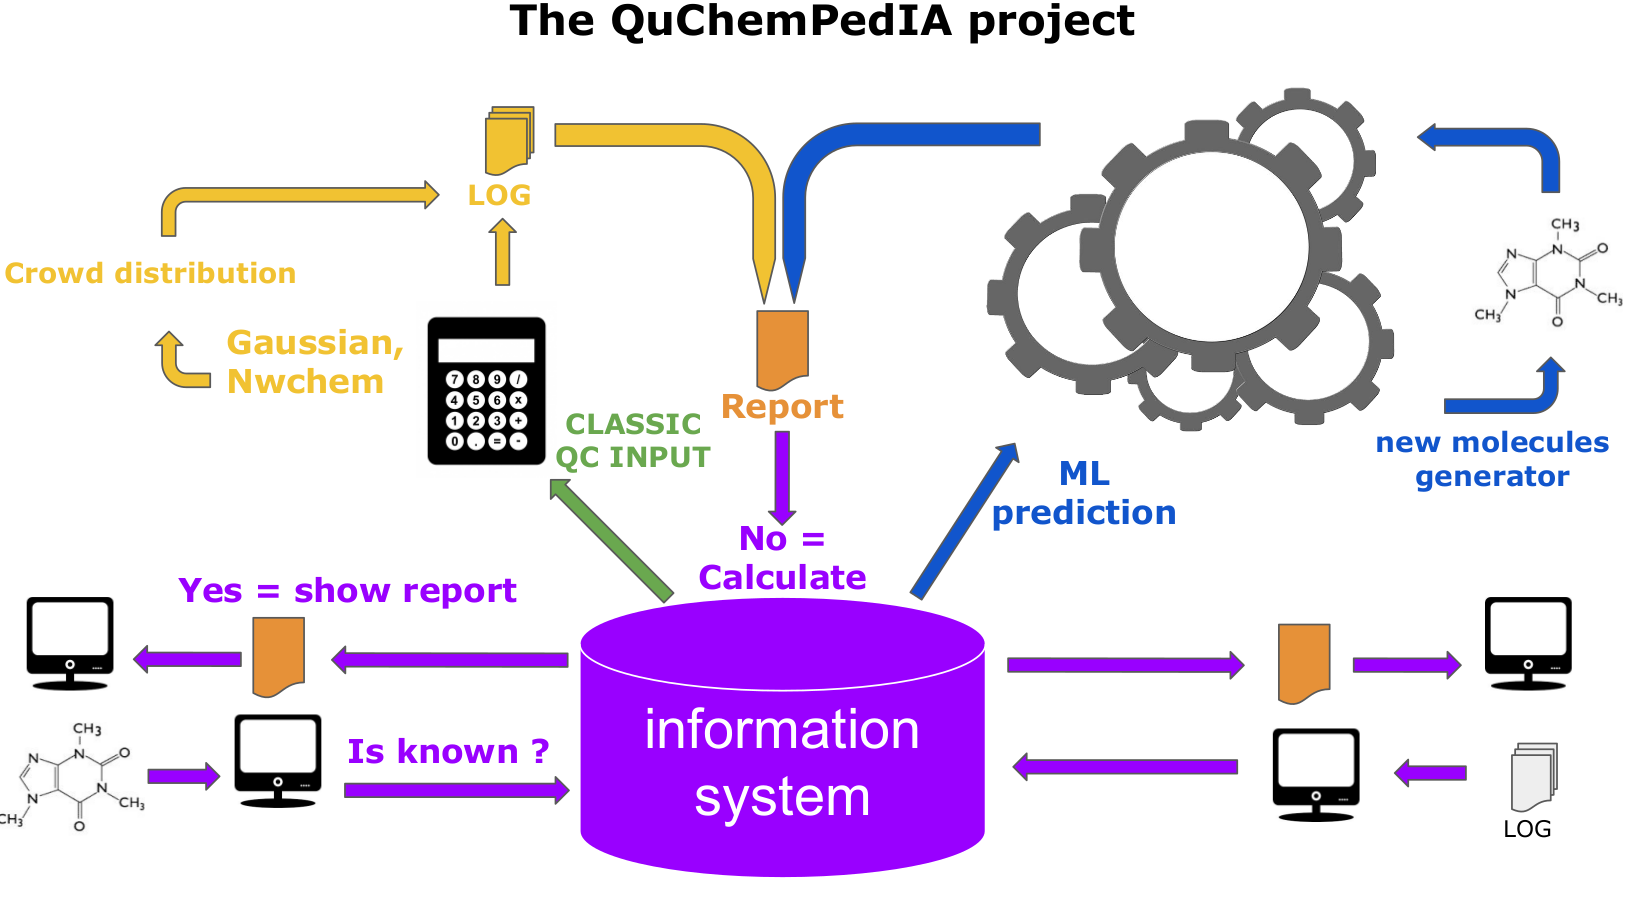
\includegraphics[scale=1]{images/part_proj.png}
	\caption{Synthèse des différents axes du projet QuChemPedia (T. Cauchy et B. Da Mota)}
	\label{figquchem}
\end{figure}

\par Il s'agit d'un projet ambitieux possédant de nombreux objectifs, représentés dans la figure \ref{figquchem}. L'objectif principal (en violet) est de mettre en place un système d'information de grande ampleur à destination des chimistes. Ce système d'information se présente sous forme d'un site web, leur permettant d'accéder à des calculs de chimie quantique.\par Ces calculs décrivent les différents états d'énergie des molécules, et représentent un second axe important (en jaune) du projet QuChemPedia. Ils sont en effet issus de divers programmes de chimie informatique (\ref{opti_geom}), dont les sorties diffèrent et sont peu structurées. Une partie importante du projet consiste alors à définir une représentation homogène des calculs provenant de ces différents programmes. Cette représentation, nommée rapport (en orange) est fournie aux utilisateurs effectuant une requête sur une molécule. Les chimistes possèdent également la possibilité de fournir les sorties des calculs qu'ils ont effectués, et d'obtenir les rapport associés.
\par Enfin, un objectif majeur du projet (en bleu) est de fournir une plus-value à ces rapports, issue de prédictions de modèles d'apprentissage automatique (\ref{apprentissage_auto}). Les calculs d'optimisation quantique sont en effet très coûteux (\ref{opti_geom}), le fait de les remplacer par des prédictions s'effectuant rapidement constituerait donc un apport très important.\\
Ce dernier axe du projet QuChemPedia est celui sur lequel j'ai travaillé cette année.



	\section{Enjeux en chimie}
		\subsection{Calcul de propriétés moléculaires}

\par Afin de pouvoir prédire les propriétés électroniques d'une molécule, les chimistes ont besoin de connaître avec une grande précision sa géométrie et certaines propriétés énergétiques. La connaissance précise de la position du nuage électronique d'une molécule dans ses différents niveaux d'énergie permet notamment de prédire les longueurs d'ondes absorbées pour un état d'énergie donné et émises lors du passage d'un état d'énergie à un autre. On peut alors prédire la couleur des molécules. \\
De plus, la connaissance précise des nuages électroniques d'un couple de molécule dans leurs états fondamentaux et excités permet de prédire leur potentiel photovoltaïque. \\

\par Les nuages électroniques moléculaires sont exprimés mathématiquement à partir de fonctions d'ondes, qui sont l'approximation par la somme de fonctions gaussiennes d'équations dont la résolution analytique est impossible avec les outils mathématiques actuels. Le calcul de ces fonctions d'ondes est donc un enjeu fondamental en chimie, et est malheureusement très coûteux en termes de puissance et de temps de calcul. Le calcul de la fonction d'ondes d'une molécule de taille moyenne (environ 50 atomes) peut en effet prendre plusieurs semaines. \\

\par Dans la figure ci-dessous, on représente les iso-niveaux de probabilité de présence des électrons d'une molécule (nuage électronique), calculés à partir de sa fonction d'ondes. On considère que les surfaces de couleurs différentes représentent la même information.\\ 

\begin{figure}[!h]
	\centering
	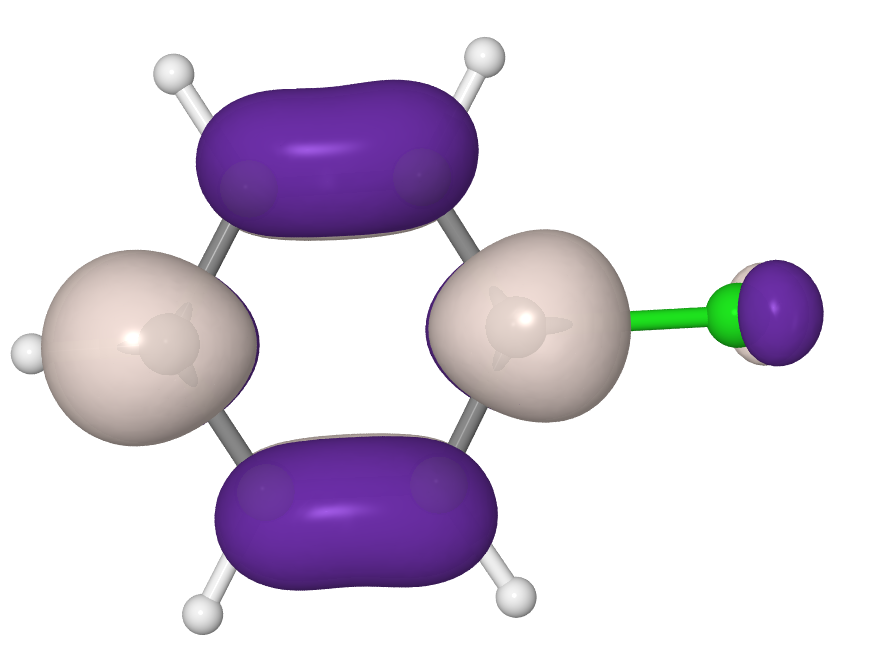
\includegraphics[scale=0.25]{images/iso_niveaux.png}
	\caption{Représentation des iso-niveaux de probabilité de présence électronique d'une molécule}
\end{figure}

\par Le calcul de la géométrie (position des atomes) et des propriétés énergétiques d'une molécule dépendent des fonctions d'ondes. Dans le cadre de ce stage, nous nous intéressons uniquement à la prédiction de géométries moléculaires optimisées (convergées), c'est pourquoi les deux parties suivantes vont décrire les approches actuellement utilisées en chimie pour calculer ces géométries. L'objectif de ces deux méthodes est de calculer une géométrie optimisée à partir d'une géométrie issue de mesures expérimentales ou de résultats théoriques.

\subsection{Mécanique moléculaire}
La mécanique moléculaire, à travers des outils comme OpenBabel\cite{openbabel} permet d'optimiser la géométrie des molécules selon des règles de distances typiques entre des couples d'atomes et d'angles typiques entre des liaisons. Il s'agit d'une approche simple qui ne permet pas d'obtenir une précision suffisante pour prédire les propriétés moléculaires. Du fait de sa rapidité, elle peut néanmoins être utilisée comme pré-traitement d'une géométrie théorique ou expérimentale et servir d'entrée à une optimisation géométrique quantique. 

\subsection{Optimisation géométrique quantique}
\par L'approche communément utilisée en chimie pour optimiser la géométrie moléculaire s'appuie sur l'optimisation itérative de la densité électronique. Elle est basée sur la \emph{Density Functional Theory} (DFT), qui propose une méthode dans laquelle la densité électronique d'une molécule est optimisée itérativement par la résolution d'équations, jusqu'à atteindre un seuil de cohérence donné. La géométrie moléculaire est alors déduite de la fonction d'onde, elle-même déduite de la densité électronique. Cette méthode est implémentée dans de nombreux programmes de chimie computationnelle, dont notamment Gaussian et Gamess.\\

\par L'inconvénient principal de cette approche est le temps de calcul nécessaire, qui limite la possibilité de l'appliquer à un grand nombre de molécules. Si l'on possédait une méthode plus rapide, on pourrait par exemple imaginer l'automatisation de la recherche de couples de molécules ayant un potentiel photovoltaïque élevé et dont la synthèse serait moins polluante que les couples utilisés actuellement, en associant à la recherche une fonction de coût qui représenterait le coût écologique de la synthèse.\\
Afin de réduire le temps d'optimisation, nous tentons de développer une solution basée sur l'élaboration de modèles d'apprentissage automatique, qui remplaceraient partiellement ou en totalité le calcul itératif de la fonction d'ondes.
	\section{Utilisation de modèles d'apprentissage automatique}
		\label{apprentissage_auto}

\subsection{Principes fondamentaux}

\label{apprentissage_automatique_principes}

L'apprentissage automatique supervisé (ou apprentissage artificiel supervisé) définit un certain nombre de méthodes permettant d'effectuer des prédictions pour résoudre des problèmes. Ces méthodes sont appelées « modèles », et correspondent aux différents algorithmes utilisés pour extraire la connaissance d'un ensemble d'exemples, puis pour effectuer des prédictions sur des exemples inconnus. Avant d'effectuer des prédictions, les modèles doivent en effet d'abord suivre une phase d'apprentissage (ou d'entraînement), pendant laquelle leurs paramètres internes sont ajustés pour effectuer la bonne prédiction en fonction des données en entrée. Dans le cas qui nous intéresse, ces prédictions peuvent être une valeur ou un ensemble de valeurs, on parle alors d'une tâche de régression. Lors de la phase d'entraînement, la distance entre la prédiction d'un modèle et la valeur cible qui était attendue pour chaque exemple lui est donnée. Ce mécanisme lui permet d'ajuster itérativement ses paramètres internes, et est à l'origine de la qualification d'apprentissage supervisé.


\subsubsection{Séparation des jeux de données}

\label{apprentissage_automatique_separation_jeux}

\par Lorsque l'on élabore un modèle prédictif, il n'est pas souhaitable d'évaluer ses performances sur les données qui ont servi à son entraînement. Cela induirait en effet un biais important, du fait qu'il est possible qu'il devienne très performant pour prédire les données qu'il connaît, mais qu'il ne soit pas capable de généraliser ses connaissances à des données qui lui sont inconnues (\ref{sur_ajustement}). C'est pour cette raison que l'on sépare généralement les données en deux jeux disjoints : un jeu d'entraînement sur lequel le modèle effectue son apprentissage, et un jeu de test (ou de validation) sur lequel ses performances sont évaluées.

\subsubsection{Validation croisée}

\label{apprentissage_automatique_validation_croisée}

\par Pour évaluer les performances d'un modèle, il est intéressant d'évaluer ses performances lorsqu'il s'entraîne sur des jeux de données différents, la qualité des prédictions d'un modèle pouvant varier d'un entraînement à un autre. Une technique répandue pour évaluer la variance des performances d'un modèle est celle de la validation croisée à $n$ entraînements. Elle consiste à séparer le jeu d'entraînement en $n$ sous-ensembles disjoints nommés plis, puis à effectuer $n$ entraînements sur toutes les combinaisons telles que $n-1$ plis constituent le jeu d'apprentissage, et le dernier pli forme le jeu de test. On peut alors étudier la performance moyenne du modèle, ainsi que la dispersion de la qualité de ses prédictions.


\subsubsection{Recherche des paramètres optimaux}

\label{apprentissage_automatique_quadri}
\par En plus des paramètres internes, les modèles présentent également un certain nombre de paramètres permettant de régler leurs représentations internes ou leurs phases d'apprentissage. Ces paramètres sont parfois appelés hyper-paramètres. Lorsque l'on élabore un modèle, il faut alors également préciser leur valeurs.\\
\par Pour déterminer un ensemble d'hyper-paramètres optimal ou du moins efficace, la technique la plus répandue est celle de la recherche par quadrillage, éventuellement avec validation croisée. Elle consiste à définir une grille de paramètres, soit un tableau à deux dimensions, contenant pour chaque paramètre (ligne) un ensemble de valeurs (colonnes). Pour chaque combinaison des valeurs, un modèle est entraîné, puis la performance relative des différents modèles est évaluée à la fin de la recherche. Dans le cas d'une recherche par quadrillage avec validation croisée à $n$ entraînements, chaque combinaison de paramètres est testée $n$ fois, ce qui permet en outre de tester la variance des performances de chaque combinaison.

\subsubsection{Prévention du sur-ajustement}
\label{sur_ajustement}

\par Lorsque les données représentent des connaissances trop simples pour un modèle, ou réciproquement que les paramètres internes d'un modèle permettent de représenter des connaissances plus complexes que celles des données, la phase d'entraînement du modèle risque de mener à sur-ajustement (ou sur-apprentissage) des données. Cela signifie que le modèle effectuera de bonnes prédictions sur les données d'entraînement, mais que les connaissances extraites par le modèle se généraliseront mal à de nouvelles données, du fait de leur trop grande spécificité aux données d'apprentissage.\\
\par Pour parer cela, les différents modèles proposent des techniques de régularisation qui leur sont propres, et qui vont permettre de limiter leur liberté à ajuster de trop près les données d'entraînement.


\subsection{Entraînement de réseaux de neurones artificiels}

\label{apprentissage_automatique_nn}

\subsubsection{Principe}
\par Les réseaux de neurones artificiels sont des modèles prédictifs qui possèdent l'avantage d'être en général plus efficaces que les autres types de modèles sur des jeux de données de grande taille. Ils ont également montré de très bonnes performances comparativement aux autres types de modèles sur des problèmes de traitement de signaux et de traitement d'images.\\

\par L'objectif de ces réseaux de neurones est d'approximer la fonction qui à chaque exemple donné en entrée associe l'ensemble de valeurs attendu en sortie. Ils sont pour cela composés d'un ensemble de neurones artificiels partageant des connexions. L'information circule de l'entrée à la sortie du modèle, en étant transformée successivement par les différents neurones, jusqu'à idéalement prendre la valeur attendue en sortie.\\

\par Chaque neurone est défini par l'ensemble des neurones dont la sortie constitue son entrée, un ensemble de poids, un seuil, une fonction d'activation, ainsi que par l'ensemble des neurones dont l'entrée contient sa sortie. Nous formalisons le fonctionnement d'un neurone de la façon suivante.\\
Soit $n$ la taille de l'entrée d'un neurone, $x_i$ sa $i$\up{ème} entrée, $w_i$ le poids associé à sa $i$\up{ème} entrée ($i \in \{1, ..., n\}$) , $\Theta$ son seuil et $\varphi$ sa fonction d'activation. La somme de $\sum\limits_{i=1}^n w_ix_i$ et de $\Theta$ est transmise à la fonction d'activation, dont la sortie $O$ constitue la sortie du neurone. La valeur $O$ est alors propagée aux neurones suivants.
Ce mécanisme est schématisé dans la figure \ref{neurone}.\\

\begin{figure}
	\centering
	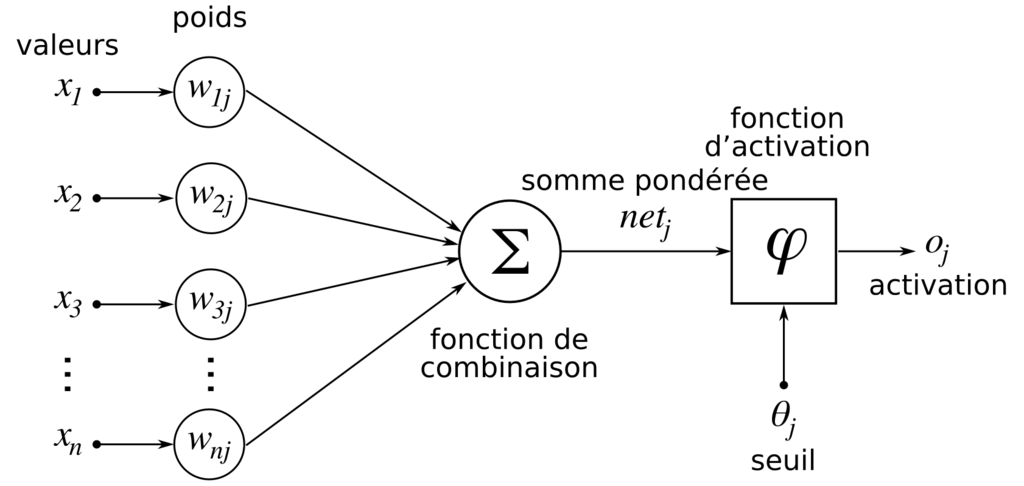
\includegraphics[scale=0.3]{images/neurone.png}
	\caption{Schématisation du fonctionnement d'un neurone artificiel (Wikimedia, Chrislb)}
	\label{neurone}
\end{figure}

\par La phase d'entraînement d'un réseau de neurones est un problème d'optimisation visant à trouver un ensemble de paramètres $w_i$ et $\Theta$ pour chaque neurone du réseau, qui minimise une fonction de coût évaluant la qualité des prédictions.

\subsubsection{Bibliothèque logicielles}

\label{apprentissage_automatique_bibli_log}

\par La totalité du code développé lors de ce projet l'a été dans le langage Python.\\

\par Pour l'implémentation des réseaux de neurones, nous utilisons la bibliothèque Tensorflow\cite{tf} développée par Google, par l'intermédiaire de la surcouche TFLearn\footnote{http://tflearn.org}, qui offre une interface simplifiée pour créer des réseaux de neurones aux architectures communes.\\

\par Nous utilisons de plus la bibliothèque Scikit-Learn\cite{sklearn}, qui permet d'automatiser un certain nombre de tâches liées à l'apprentissage automatique.\\

\par Nous utilisons en outre l'interface web Tensorboard, incluse dans Tensorflow, qui permet de visualiser l'évolution des différentes métriques évaluant la qualité des modèles au cours de l'entraînement.\\

\par Enfin, nous utilisons les notebooks Jupyter\cite{jupyter}, qui permettent d'expérimenter simplement des algorithmes de génération de données ou d'entraînement de modèles, et de présenter les résultats de manière claire.

\subsubsection{Hyper-paramètres}

\label{apprentissage_automatique_parametres_nn}

\par Les modèles crées par l'intermédiaire de TFLearn présentent un certain nombre d'hyper-paramètres (\ref{apprentissage_automatique_principes}), qui permettent de régler finement les modèles que l'on entraîne. Nous listons ci-dessous ces différents paramètres et leurs rôles.

\paragraph{Optimiseur : } Définit la méthode d'optimisation des poids utilisée à chaque étape de l'entraînement. Nous utilisons pour tous les modèles l'optimiseur Adam\cite{adam}, réputé pour être efficace et éviter les minimums locaux de la fonction de coût.

\paragraph{Taux d'apprentissage (\emph{learning rate}) : } Définit la vitesse maximale à laquelle l'optimiseur va modifier les solutions pendant l'optimisation des poids lors de l'entraînement des modèles. Si la valeur est trop faible, l'entraînement mettra trop de temps à converger vers de bonnes solutions. Si elle est trop élevée, le modèle risque d'être bloqué dans des minimums locaux de la fonction de coût.

\paragraph{Epsilon : } Paramètre de l'optimiseur Adam.

\paragraph{Taille de lot (\emph{batch size)} :} L'apprentissage des réseaux de neurones artificiels ne s'effectue pas exemple par exemple mais lot d'exemples par lot d'exemples. Ce paramètre définit la taille de ces lots.

\paragraph{Époques (\emph{epochs})} : Définit le nombre d'époques d'entraînement. Cela correspond au nombre de fois que le réseau de neurones va apprendre sur toutes les données du jeu d'entraînement.

\paragraph{Initialisation des poids : } Les poids du réseau de neurones doivent être initialisés à des valeurs non nulles pour que l'information puisse se propager. Ce paramètre correspond à l'écart-type de la variable aléatoire gaussienne utilisée pour initialiser les poids.

\paragraph{Fonctions d'activation : } Définit les fonctions d'activation utilisées par les neurones artificiels. On différencie la fonction utilisée par les neurones des couches internes de la fonction utilisée par les neurones de la couche de sortie.

\paragraph{Dégradation des poids (\emph{weight decay}) : } Il s'agit d'un paramètre de régularisation ajoutant un terme à la fonction de coût, qui va forcer les poids à ne pas prendre de valeurs trop élevées. La présence de poids possédant des valeurs élevées est en effet un facteur de sur-ajustement\cite{weight_decay}.

\paragraph{Taux d'abandon (\emph{dropout}) : } Technique de régularisation permettant d'éviter le sur-ajustement. À chaque époque d'entraînement, certains neurones sont désactivés aléatoirement afin de pousser le modèle à être résilient et à éviter qu'une co-dépendance forte entre certains neurones s'installe. Ce paramètre permet en réalité de définir la proportion de neurones qui resteront activés à chaque époque.




		
\chapter{Représentations géométriques moléculaires}
	\section{Matrice des coordonnées atomiques}
		\par La matrice des coordonnées atomiques est la façon la plus simple de représenter la géométrie d'une molécule. L'intérêt de cette représentation est qu'elle est utilisée par les chimistes (fichiers .mol, .xyz + utilisation dans les logiciels de calcul ?). Il s'agit donc pour nous d'une représentation d'entrée et de sortie. Nos données d'apprentissage contiennent pour chaque molécule une matrice des positions, en plus des numéros et masses atomiques, et nous devons être capables de fournir cette représentation en sortie de nos prédictions, pour que nos résultats soient utilisables par les chimistes.\\

\par Formellement, la matrice des coordonnées atomiques d'une molécule contient les coordonnées de chaque atome dans un repère cartésien orthonormé à trois dimensions.

\begin{figure}[!h]
	\centering
	
	\begin{tabular}{|c|c|c|}
		\hline
		$\boldsymbol{x_1}$ & $\boldsymbol{y_1}$ & $\boldsymbol{z_1}$ \\ \hline	
		$\boldsymbol{x_2}$ & $\boldsymbol{y_2}$ & $\boldsymbol{z_2}$ \\ \hline	
		\textbf{\rot{... }} & \textbf{\rot{... }} & \textbf{\rot{... }}\\ \hline 	
		$\boldsymbol{x_n}$ & $\boldsymbol{y_n}$ & $\boldsymbol{z_n}$ \\ \hline	
	\end{tabular}

	\caption{Matrice des coordonnées atomiques (molécule de taille $n$)}
\end{figure}

\par Si cette représentation de la géométrie des molécules est très commode pour les chimistes, elle n'est pas utilisable telle quelle dans nos modèles prédictifs. Nous cherchons en effet à prédire des distances (ou des différences de distances, voir REF DELTA\_DIST...) entre des points. Donner les coordonnées  brutes aux modèles implique qu'ils devraient \emph{apprendre} les outils mathématiques permettant de calculer des distances entre des points, ce qui constitue en soi une tâche complexe. C'est pourquoi nous allons définir un ensemble de représentations géométriques, toutes basées sur les distances plutôt que les positions, et adaptées aux différentes prédictions que nous souhaitons effectuer.

	\section{Matrice réduite des distances inter-atomiques}
		\subsection{Motivation}

\par Cette représentation est issue du travail qui a été fait précédemment sur ce projet, et consiste à représenter une molécule par ses distances inter-atomiques. L'intérêt de cette représentation est que les réseaux de neurones qui l'utilisent travaillent dans des repères relatifs. Lorsqu'ils effectuent des prédictions, ils n'ont pas besoin de \textit{comprendre} les notions mathématiques de géométrie permettant de déduire la position d'un point dans un repère à partir de ses distances à d'autres points, contrairement à la représentation décrite en (REF REPR ABS). Cette représentation est donc très commode pour les modèles prédictifs dont l'objectif est de corriger les distances entre deux atomes, puisqu'elle est basée sur les distances entre les paires d'atomes.

\par De plus, l'utilisation d'une représentation basée sur les distances relatives permet d'offrir une représentation unique pour les molécules ayant des ensembles d'atomes pouvant effectuer des rotations, contrairement aux représentations basées sur les coordonnées (REF REPR COORDS) ou sur des distances à des points fixes (REF REPR DIST ABS).

\par Lorsque les modèles utilisent cette représentation en sortie, ou plus précisément que l'on déduit la matrice réduite des distances inter-atomiques de la sortie du modèle (voir REF SORTIE DELTA\_DIST+H), nous devons toutefois trouver une méthode (voir REF PRINC RECONSTRUCT) pour reconstruire les molécules sous la forme d'une matrice de coordonnées (REF REPR COORDS).

\subsection{Formalisation}

\par Pour ne pas surcharger les modèles d'information, nous ne travaillons pas sur la matrice de distances inter-atomiques complète, mais sur un sous-ensemble de cardinalité minimale de cette matrice telle que nous pouvons reconstruire sans ambiguïté un ensemble de coordonnées représentant les positions des atomes de la molécule. La matrice des distances étant symétrique et la diagonale étant nulle, toute l'information est contenue dans chaque demi-matrice triangulaire privée de la diagonale. \\

\begin{figure}[h!]
	\centering
	
	
	\begin{tabular}{c|c|c|c|c|c|c|c|c|c|c|c|c}
	    & a\textsubscript{0} & a\textsubscript{1} & a\textsubscript{2} & a\textsubscript{3} & a\textsubscript{4} & ... & a\textsubscript{n-4} & a\textsubscript{n-3} & a\textsubscript{n-2} & 
	    	 a\textsubscript{n-1}  & a\textsubscript{n}\\ \hline
		a\textsubscript{0} & \textbf{d\textsubscript{0,0}} & \textbf{d\textsubscript{0,1}} & \textbf{d\textsubscript{0,2}} & 
		    \textbf{d\textsubscript{0,3}} & \textbf{d\textsubscript{0,4}} & \textbf{...} & \textbf{d\textsubscript{0,n-4}} & 
		    \textbf{d\textsubscript{0,n-3}} & \textbf{d\textsubscript{0,n-2}} & \textbf{d\textsubscript{0,n-1}}
		    & \textbf{d\textsubscript{0,n}} \\ \hline
		a\textsubscript{1} & \textbf{d\textsubscript{1,0}} & \textbf{d\textsubscript{1,1}} & \textbf{d\textsubscript{1,2}} & 
			\textbf{d\textsubscript{1,3}} & \textbf{d\textsubscript{1,4}} & \textbf{...} & \textbf{d\textsubscript{1,n-4}} & 
			\textbf{d\textsubscript{1,n-3}} & \textbf{d\textsubscript{1,n-2}} & \textbf{d\textsubscript{1,n-1}} & 
			\textbf{d\textsubscript{1,n}} \\ \hline
		a\textsubscript{2} & \textbf{d\textsubscript{2,0}} & \textbf{d\textsubscript{2,1}} & \textbf{d\textsubscript{2,2}} &
			\textbf{d\textsubscript{2,3}} & \textbf{d\textsubscript{2,4}} & \textbf{...} & \textbf{d\textsubscript{2,n-4}} & 
			\textbf{d\textsubscript{2,n-3}} & \textbf{d\textsubscript{2,n-2}} & \textbf{d\textsubscript{2,n-1}} & 
			\textbf{d\textsubscript{2,n}} \\ \hline
		a\textsubscript{3} & \textbf{d\textsubscript{3,0}} & \textbf{d\textsubscript{3,1}} & \textbf{d\textsubscript{3,2}} & 
			\textbf{d\textsubscript{3,3}} & \textbf{d\textsubscript{3,4}} & \textbf{...} & \textbf{d\textsubscript{3,n-4}} & 
			\textbf{d\textsubscript{3,n-3}} & \textbf{d\textsubscript{3,n-2}} & \textbf{d\textsubscript{3,n-1}} & 
			\textbf{d\textsubscript{3,n}} \\ \hline
		a\textsubscript{4} & \textbf{d\textsubscript{4,0}} & \textbf{d\textsubscript{4,1}} & \textbf{d\textsubscript{4,2}} & 
			\textbf{d\textsubscript{4,3}} & \textbf{d\textsubscript{4,4}} & \textbf{...} & \textbf{d\textsubscript{4,n-4}} & 
			\textbf{d\textsubscript{4,n-3}} & \textbf{d\textsubscript{4,n-2}} & \textbf{d\textsubscript{4,n-1}} & 
			\textbf{d\textsubscript{4,n}} \\ \hline
			
		\rot{... } & \textbf{\rot{... }} & \textbf{\rot{... }} & \textbf{\rot{... }} & \textbf{\rot{... }} & 
		\textbf{\rot{... }} & \textbf{\halfrot{ ... }} & \textbf{\rot{... }} & \textbf{\rot{... }} & \textbf{\rot{... }} & 
		\textbf{\rot{... }} & \textbf{\rot{... }} \\ \hline


		a\textsubscript{n-4} & \textbf{d\textsubscript{n-4,0}} & \textbf{d\textsubscript{n-4,1}} & \textbf{d\textsubscript{n-4,2}} & 
			\textbf{d\textsubscript{n-4,3}} & \textbf{d\textsubscript{n-4,4}} & \textbf{...} & \textbf{d\textsubscript{n-4,n-4}} & 
			\textbf{d\textsubscript{n-4,n-3}} & \textbf{d\textsubscript{n-4,n-2}} & \textbf{d\textsubscript{n-4,n-1}} & 
			\textbf{d\textsubscript{n-3,n}} \\ \hline

		a\textsubscript{n-3} & \textbf{d\textsubscript{n-3,0}} & \textbf{d\textsubscript{n-3,1}} & \textbf{d\textsubscript{n-3,2}} & 
			\textbf{d\textsubscript{n-3,3}} & \textbf{d\textsubscript{n-3,4}} & \textbf{...} & \textbf{d\textsubscript{n-3,n-4}} & 
			\textbf{d\textsubscript{n-3,n-3}} & \textbf{d\textsubscript{n-3,n-2}} & \textbf{d\textsubscript{n-3,n-1}} & 
			\textbf{d\textsubscript{n-3,n}} \\ \hline
		a\textsubscript{n-2} & \textbf{d\textsubscript{n-2,0}} & \textbf{d\textsubscript{n-2,1}} & \textbf{d\textsubscript{n-2,2}} & 
			\textbf{d\textsubscript{n-2,3}} & \textbf{d\textsubscript{n-2,4}} & \textbf{...} & \textbf{d\textsubscript{n-2,n-4}} & 
			\textbf{d\textsubscript{n-2,n-3}} & \textbf{d\textsubscript{n-2,n-2}} & \textbf{d\textsubscript{n-2,n-1}} & 
			\textbf{d\textsubscript{n-2,n}} \\ \hline
		a\textsubscript{n-1} & \textbf{d\textsubscript{n-1,0}} & \textbf{d\textsubscript{n-1,1}} & \textbf{d\textsubscript{n-1,2}} & 
			\textbf{d\textsubscript{n-1,3}} & \textbf{d\textsubscript{n-1,4}} & \textbf{...} & \textbf{d\textsubscript{n-1,n-4}} & 
			\textbf{d\textsubscript{n-1,n-3}} & \textbf{d\textsubscript{n-1,n-2}} & \textbf{d\textsubscript{n-1,n-1}} & 
			\textbf{d\textsubscript{n-1,n}} \\ \hline
		a\textsubscript{n} & \textbf{d\textsubscript{n,0}} & \textbf{d\textsubscript{n,1}} & \textbf{d\textsubscript{n,2}} & 
			\textbf{d\textsubscript{n,3}} & \textbf{d\textsubscript{n,4}} & \textbf{...} & \textbf{d\textsubscript{n,n-4}} & 
			\textbf{d\textsubscript{n,n-3}} & \textbf{d\textsubscript{n,n-2}} & \textbf{d\textsubscript{n,n-1}} & 
			\textbf{d\textsubscript{n,n}} \\ \hline
		
	\end{tabular}

	
	\caption{Matrice complète des distances inter-atomiques d'une molécule}
\end{figure}

\par De plus, nous n'avons besoin que des distances à quatre points pour retrouver la position de chaque atome (voir REF RECONSTRUCT), nous nous contentons donc de garder les quatre premières distances de chaque ligne de la matrice triangulaire supérieure privée de la diagonale.


\begin{figure}[h!]
	\centering
	
	
	\begin{tabular}{c|c|c|c|c|c|c|c|c|c|c|c|c}
	    & a\textsubscript{0} & a\textsubscript{1} & a\textsubscript{2} & a\textsubscript{3} & a\textsubscript{4} & ... & a\textsubscript{n-4} & a\textsubscript{n-3} & a\textsubscript{n-2} & 
	    	 a\textsubscript{n-1}  & a\textsubscript{n}\\ \hline
		a\textsubscript{0} & d\textsubscript{0,0} & \textbf{d\textsubscript{0,1}} & \textbf{d\textsubscript{0,2}} & 
		    \textbf{d\textsubscript{0,3}} & \textbf{d\textsubscript{0,4}} & ... & d\textsubscript{0,n-4} & 
		    d\textsubscript{0,n-3} & d\textsubscript{0,n-2} & d\textsubscript{0,n-1}
		    & d\textsubscript{0,n} \\ \hline
		a\textsubscript{1} & d\textsubscript{1,0} & d\textsubscript{1,1} & \textbf{d\textsubscript{1,2}} & 
			\textbf{d\textsubscript{1,3}} & \textbf{d\textsubscript{1,4}} & ... & d\textsubscript{1,n-4} & 
			d\textsubscript{1,n-3} & d\textsubscript{1,n-2} & d\textsubscript{1,n-1} & 
			d\textsubscript{1,n} \\ \hline
		a\textsubscript{2} & d\textsubscript{2,0} & d\textsubscript{2,1} & d\textsubscript{2,2} &
			\textbf{d\textsubscript{2,3}} & \textbf{d\textsubscript{2,4}} & ... & d\textsubscript{2,n-4} & 
			d\textsubscript{2,n-3} & d\textsubscript{2,n-2} & d\textsubscript{2,n-1} & 
			d\textsubscript{2,n} \\ \hline
		a\textsubscript{3} & d\textsubscript{3,0} & d\textsubscript{3,1} & d\textsubscript{3,2} & 
			d\textsubscript{3,3} & \textbf{d\textsubscript{3,4}} & ... & d\textsubscript{3,n-4} & 
			d\textsubscript{3,n-3} & d\textsubscript{3,n-2} & d\textsubscript{3,n-1} & 
			d\textsubscript{3,n} \\ \hline
			
		a\textsubscript{4} & d\textsubscript{4,0} & d\textsubscript{4,1} & d\textsubscript{4,2} & 
			d\textsubscript{4,3} & \textbf{d\textsubscript{4,4}} & ... & d\textsubscript{4,n-4} & 
			d\textsubscript{4,n-3} & d\textsubscript{4,n-2} & d\textsubscript{4,n-1} & 
			d\textsubscript{4,n} \\ \hline
			
		\rot{... } & \rot{... } & \rot{... } & \rot{... } & \rot{... } & 
		\rot{... } & \halfrot{ ... } & \rot{... } & \rot{... } & \rot{... } & 
		\rot{... } & \rot{... } \\ \hline
	    	
	    	
		a\textsubscript{n-4} & d\textsubscript{n-4,0} & d\textsubscript{n-4,1} & d\textsubscript{n-4,2} & 
			d\textsubscript{n-4,3} & d\textsubscript{n-4,4} & ... & d\textsubscript{n-4,n-4} & 
			\textbf{d\textsubscript{n-4,n-3}} & \textbf{d\textsubscript{n-4,n-2}} & \textbf{d\textsubscript{n-4,n-1}} & 
			\textbf{d\textsubscript{n-4,n}} \\ \hline	    
		a\textsubscript{n-3} & d\textsubscript{n-3,0} & d\textsubscript{n-3,1} & d\textsubscript{n-3,2} & 
			d\textsubscript{n-3,3} & d\textsubscript{n-3,4} & ... & d\textsubscript{n-3,n-4} & 
			d\textsubscript{n-3,n-3} & \textbf{d\textsubscript{n-3,n-2}} & \textbf{d\textsubscript{n-3,n-1}} & 
			\textbf{d\textsubscript{n-3,n}} \\ \hline
		a\textsubscript{n-2} & d\textsubscript{n-2,0} & d\textsubscript{n-2,1} & d\textsubscript{n-2,2} & 
			d\textsubscript{n-2,3} & d\textsubscript{n-2,4} & ... & d\textsubscript{n-2,n-4} & 
			d\textsubscript{n-2,n-3} & d\textsubscript{n-2,n-2} & \textbf{d\textsubscript{n-2,n-1}} & 
			\textbf{d\textsubscript{n-2,n}} \\ \hline
		a\textsubscript{n-1} & d\textsubscript{n-1,0} & d\textsubscript{n-1,1} & d\textsubscript{n-1,2} & 
			d\textsubscript{n-1,3} & d\textsubscript{n-1,4} & ... & d\textsubscript{n-1,n-4} & 
			d\textsubscript{n-1,n-3} & d\textsubscript{n-1,n-2} & d\textsubscript{n-1,n-1} & 
			\textbf{d\textsubscript{n-1,n}} \\ \hline
		a\textsubscript{n} & d\textsubscript{n,0} & d\textsubscript{n,1} & d\textsubscript{n,2} & 
			d\textsubscript{n,3} & d\textsubscript{n,4} & ... & d\textsubscript{n,n-4} & 
			d\textsubscript{n,n-3} & d\textsubscript{n,n-2} & d\textsubscript{n,n-1} & d\textsubscript{n,n} \\ \hline
		
	\end{tabular}

	
	\caption{Matrice réduite des distances inter-atomiques d'une molécule (en gras)}
\end{figure}

\begin{figure}[h!]
	\centering
	
	
	\begin{tabular}{|c|c|c|c|}
		\hline
		\textbf{d\textsubscript{0,1}} & \textbf{d\textsubscript{0,2}} & \textbf{d\textsubscript{0,3}} & \textbf{d\textsubscript{0,4}} \\ \hline
		\textbf{d\textsubscript{1,2}} & \textbf{d\textsubscript{1,3}} & \textbf{d\textsubscript{1,4}} & \textbf{d\textsubscript{1,5}} \\ \hline
		\textbf{d\textsubscript{2,3}} & \textbf{d\textsubscript{2,4}} & \textbf{d\textsubscript{2,5}} & \textbf{d\textsubscript{2,6}} \\ \hline
		\textbf{d\textsubscript{3,4}} & \textbf{d\textsubscript{3,5}} & \textbf{d\textsubscript{3,6}} & \textbf{d\textsubscript{3,7}} \\ \hline
		\textbf{\rot{... }} & \textbf{\rot{... }} & \textbf{\rot{... }} & \textbf{\rot{... }} \\ \hline
		\textbf{d\textsubscript{n-4,n-3}} & \textbf{d\textsubscript{n-4,n-2}} & \textbf{d\textsubscript{n-4,n-1}} & \textbf{d\textsubscript{n-4,n}} \\ \hline
		\textbf{d\textsubscript{n-3,n-2}} & \textbf{d\textsubscript{n-3,n-1}} & \textbf{d\textsubscript{n-3,n}} & \textbf{0} \\ \hline
		\textbf{d\textsubscript{n-2,n-1}} & \textbf{d\textsubscript{n-2,n}} & \textbf{0} & \textbf{0} \\ \hline
		\textbf{d\textsubscript{n-1,n}} & \textbf{0} & \textbf{0} & \textbf{0} \\ \hline
	\end{tabular}

	
	\caption{Matrice réduite des distances inter-atomiques d'une molécule}
\end{figure}

\newpage
\subsection{Reconstruction des molécules}

\par Lorsqu'un modèle a pour sortie une matrice réduite des distances inter-atomiques lorsqu'il effectue des prédictions, il faut définir une méthode pour reconstruire une matrice des coordonnées (ref REPR MAT COORDS) de façon automatique à partir de cette sortie, la seule contrainte étant que la distance relative entre chaque paire d'atomes soit respectée. Il ne s'agit pour autant pas d'une tâche triviale, elle s'est en effet avérée impossible en pratique pour les grosses molécules à cause de la propagation des erreurs qu'elle induit (voir REF PROPAG ERREURS).

\subsubsection{Formalisation de la méthode de reconstruction}

\paragraph{Nécessité et limite de l'introduction d'un atome fictif} Notre méthode de reconstruction des atomes doit permettre de respecter la chiralité\footnote{Un composé chimique est dit chiral s'il n'est pas superposable à son image dans un miroir. (\url{https://fr.wikipedia.org/wiki/Chiralité_(chimie))}} des molécules. Or, en déduisant uniquement la position d'un atome de ses distances aux quatre atomes précédents, il existe des cas pour lesquels il existe plusieurs solutions pour la position de l'atome (deux si les quatre atomes précédents sur un même plan ou une infinité si les quatre atomes précédents appartiennent à une droite). Pour pallier ce problème, la méthode retenue précédemment a été d'introduire un nouveau point (que l'on nomme atome fictif) et que l'on place arbitrairement dans la molécule, à une position telle qu'il n'appartient pas au plan formé par les trois premiers atomes, ou à la droite formée par les trois premiers atomes s'ils sont alignés. De cette façon, les atomes suivants seront placés sans ambiguïté.\\
Cependant, on peut imaginer des cas pour lesquels la technique de l'introduction d'un atome fictif ne permet pas de lever l'ambiguïté, notamment pour les molécules possédant une chaîne de carbones liés par des doubles liaisons (et formant donc une droite). La méthode ne permettra pas dans ce cas de déterminer les positions des atomes en bout de chaîne tel que leurs distances relatives soient respectées, cette information étant perdue lors de la création de la matrice réduite des distances inter-atomiques. \\
Cette représentation n'est donc pas viable en pratique. Cela fait partie des raisons (voir également REF PB SQRT) pour lesquelles nous sommes passés à la représentation par matrice réduite des distances à des points fixes (REF MATR RED FIXES).

\paragraph{Placement de l'atome fictif} Puisque l'on définit la position de chaque atome en fonction de ses distances aux quatre atomes précédents, on doit d'abord placer les quatre premiers atomes de façon partiellement arbitraire. Le premier atome de la molécule dans notre représentation étant l'atome fictif a\indice{0}, nous commençons par le placer à la position qui lui a été attribuée.

\paragraph{Placement de l'atome a\indice{1}} Une fois l'atome a\indice{0} placé, il existe une infinité de solutions pour la position de l'atome a\indice{1}. On peut en effet le placer à tout point appartenant à la surface de la sphère de centre a\indice{0} et de rayon d\indice{0,1}.



\paragraph{Placement de l'atome a\indice{2}} L'atome a\indice{2} appartient au cercle solution de l'intersection entre les sphères de centres a\indice{0} et a\indice{1} et de rayons d\indice{0,2} et d\indice{1,2}. On choisit donc arbitrairement une position appartenant à ce cercle.



\paragraph{Placement de l'atome a\indice{3}} Dans le cas général, il existe deux solutions pour le placement de l'atome a\indice{3}, l'intersection non nulle de trois sphères étant deux points si tous les points ne sont pas sur un même plan ou une même droite. On choisit arbitrairement un point parmi ces deux solutions, car il n'y a pas à ce stade d'ambiguïté de chiralité de la molécule, une molécule composée de trois atomes ne possédant pas de chiralité (l'atome fictif a\indice{0} ne fait pas partie de la molécule).


\paragraph{Placement de l'atome a\indice{n}} Pour placer l'atome a\indice{$n$} ($n$ étant strictement inférieur à la taille de la molécule), nous généralisons la méthode de placement de l'atome a\indice{3}. Plutôt que de travailler sur l'intersection de quatre sphères, nous travaillons toujours sur l'intersection de trois sphères et nous utilisons la dernière distance pour discriminer les deux solutions obtenues. Cela facilite grandement la résolution des équations mathématiques associées et permet d'obtenir des solutions sensiblement équivalentes. \\
Formellement, nous calculons les positions des deux points solutions de l'intersection des trois sphères de centres a\indice{n-4}, a\indice{n-3}, et a\indice{n-2} et de rayons d\indice{n-4,n}, d\indice{n-3,n} et d\indice{n-2,n}, et nous discriminons les deux solutions selon la distance d\indice{n-1,n}. 

\begin{figure}
	\centering
	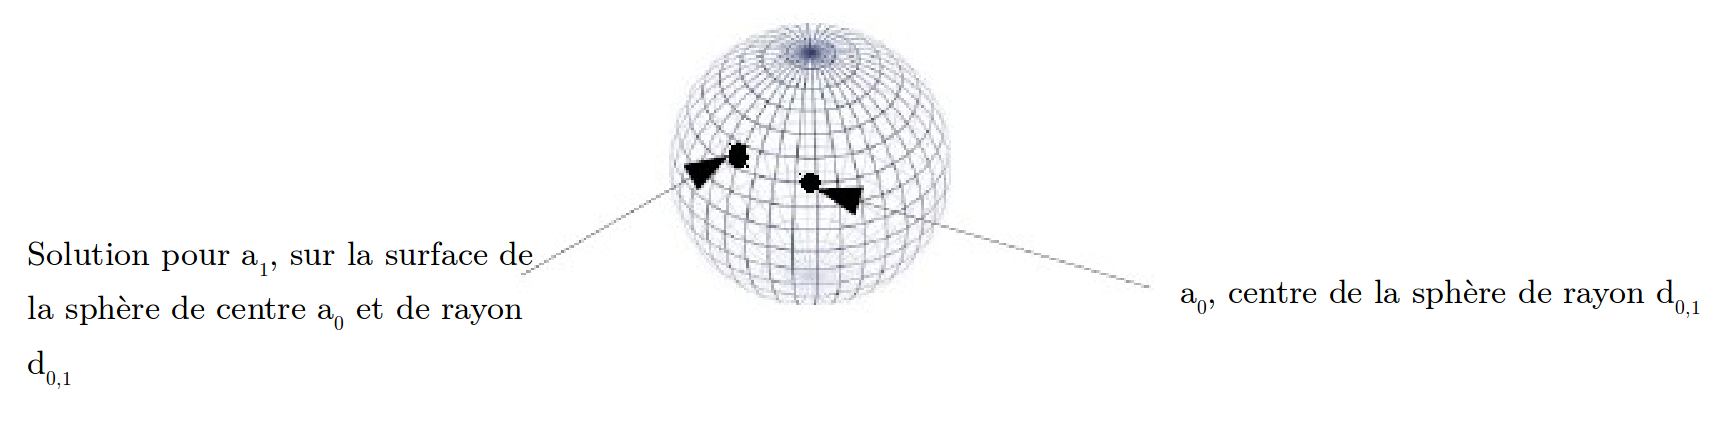
\includegraphics[scale=0.27]{images/1_sphere.png}
	\caption{Placement de l'atome a\indice{1} (image extraite du rapport de N.Roux)}
\end{figure}

\begin{figure}
	\centering
	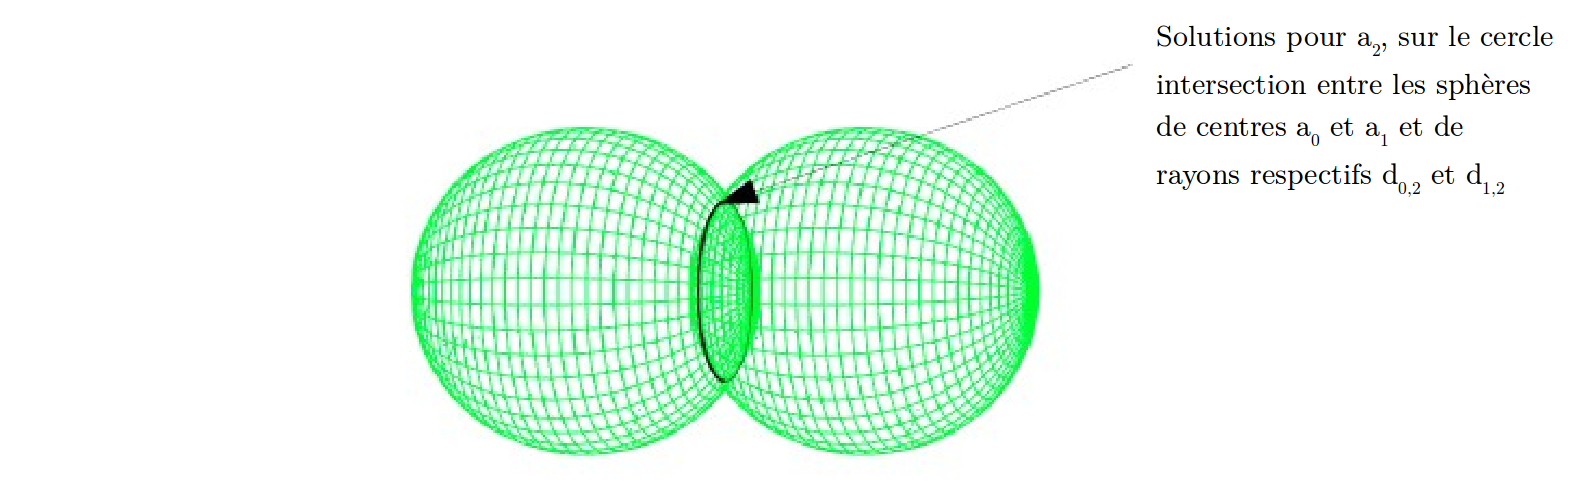
\includegraphics[scale=0.3]{images/2_spheres.png}
	\caption{Placement de l'atome a\indice{2} (image extraite du rapport de N.Roux)}
\end{figure}


\begin{figure}
	\centering
	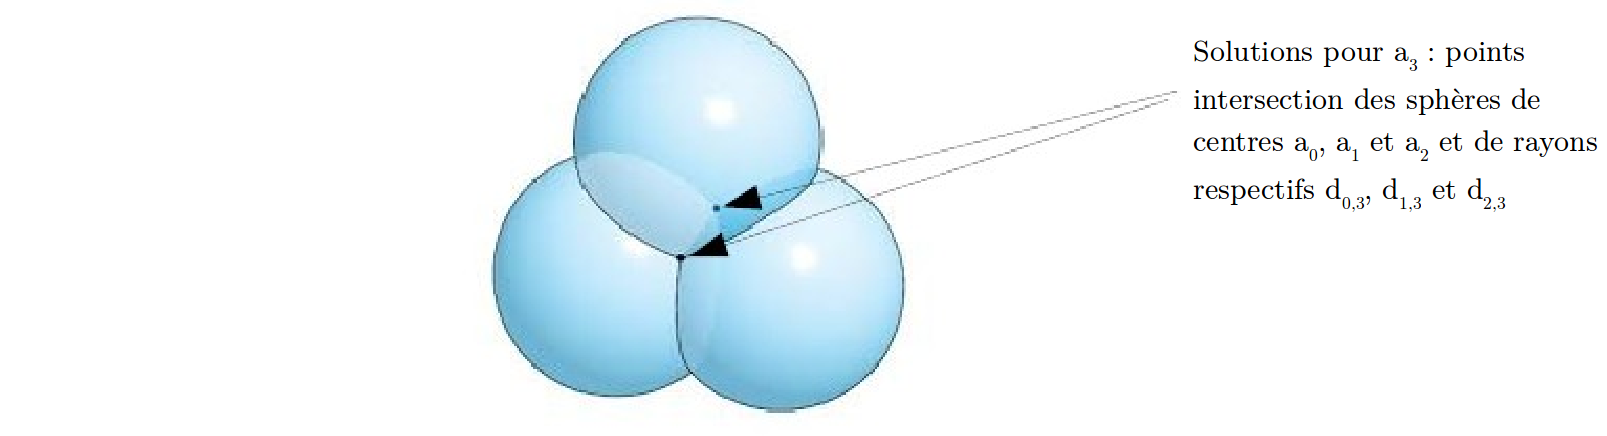
\includegraphics[scale=0.3]{images/3_spheres.png}
	\caption{Placement de l'atome a\indice{3} (image extraite du rapport de N.Roux)}
\end{figure}


\begin{figure}
	\centering
	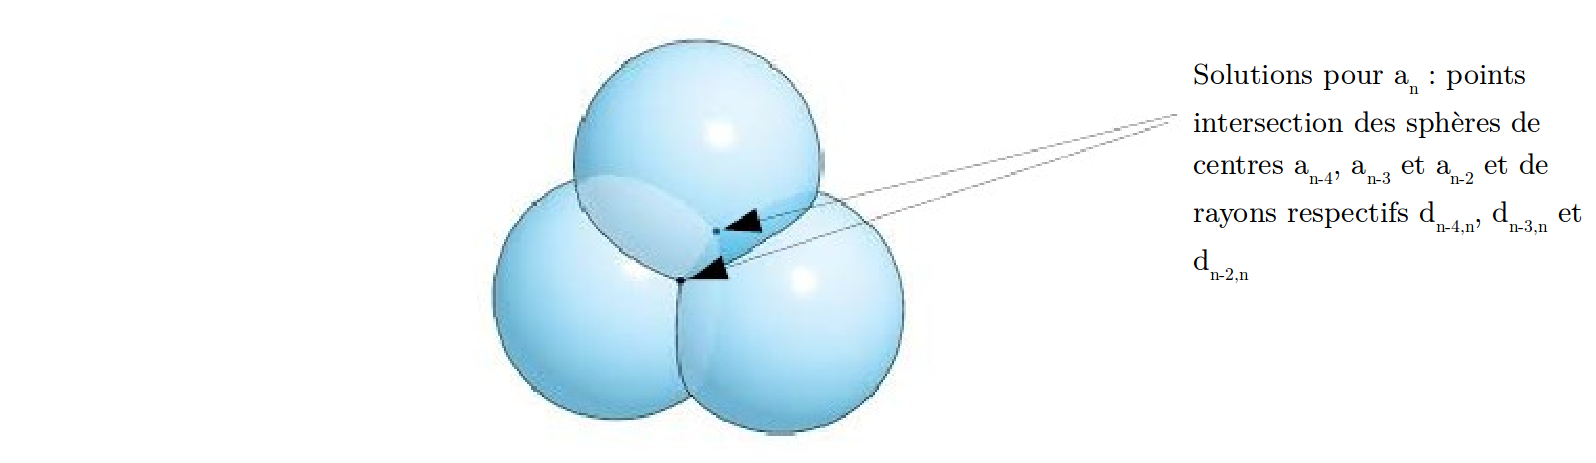
\includegraphics[scale=0.3]{images/3_spheres_gen.png}
	\caption{Placement de l'atome a\indice{n} (image extraite du rapport de N.Roux)}
\end{figure}

\subsubsection{Reconstruction automatique des positions en utilisant un solveur}

\par Nous développons ici une méthode permettant de déterminer les coordonnées d'un atome quelconque en utilisant un solveur d'équations non linéaires \footnote{\url{https://en.wikipedia.org/wiki/Nonlinear_system}}. Nous utilisons la bibliothèque Sympy\footnote{\url{http://www.sympy.org/fr/}}.\\

\par Tout d'abord, l'atome fictif a\indice{0} doit être placé à la position qui lui a été attribuée (REF PLACEMENT AT FICTIF). Nous plaçons ensuite arbitrairement les trois atomes suivants, de sorte que leurs distances relatives soient respectées. Pour simplifier le problème, nous effectuons une translation temporaire telle que a\indice{0}$'$ est à l'origine du repère. Nous plaçons alors a\indice{1}$'$ sur l'axe $x$, à une distance d\indice{0,1} de l'origine, et a\indice{2}$'$ sur le plan tel que $z=0$, à une position telle que les distances d\indice{0,2} et d\indice{1,2} sont respectées. Pour finir, nous plaçons a\indice{3}$'$ à l'une des deux solutions de l'intersection des sphères associées au problème (REF PLACEMENT A3). Le choix de la solution est arbitraire car la reconstruction de la bonne chiralité de la molécule ne dépend pas du placement des trois premiers atomes non fictifs.\\



\begin{figure}[!h]
	\centering
	
	\[
	a_{0}'\left \{
   	\begin{array}{l}
      x_{0}'=0\\
      y_{0}'=0\\
	  z_{0}'=0
   	\end{array}
   	\right .
   	\:
   	a_{1}'\left \{
   	\begin{array}{l}
      x_{1}'=d_{0,1}\\
      y_{1}'=0\\
	  z_{1}'=0
   	\end{array}
   	\right .
   	\:
	a_{2}'\left \{
   	\begin{array}{l}
      x_{2}'=\frac{d_{0,2}^2 - d_{1,2}^2 + x_{1}^2}{2x_{1}'}\\
      y_{2}'=\sqrt{d_{2,0}^2 - x_{2}'^2}\\
	  z_{2}'=0
   	\end{array}
   	\right .
   	\:
   	a_{3}'\left \{
   	\begin{array}{l}
      x_{3}'=\frac{d_{0,3}^2+x_1'^2-d_{1,3}^2}{2x_{1}'}\\
      y_{3}'=\frac{-2x_3'x_2'+d_{0,2}^2-d_{2,3}^2+d_{0,3}^2}{2y_2'}\\
	  z_{3}'=\sqrt{-x_3'^2-y_3'^2+d_{0,3}^2}
   	\end{array}
   	\right .
	\]
		
	\caption{Placement des atomes a\indice{0}$'$, a\indice{1}$'$, a\indice{2}$'$ et a\indice{3}$'$}
\end{figure}


\par Une fois que les quatre premiers atomes sont placés, nous leur appliquons une translation selon le vecteur $\vec{a_0}$, de sorte que l'atome fictif soit à sa position originale, et que les distances relatives des atomes a\indice{0}, a\indice{1}, a\indice{2} et a\indice{3} soient toujours consistantes. Nous faisons alors appel au solveur pour résoudre les équations associées au placement des autres atomes de de la molécule. Pour chaque atome, nous sélectionnons la solution respectant au mieux la distance d\indice{n-1,n} (REF PLACEMENT AN).


\begin{figure}[!h]
	\centering
	
	\[
	\left \{
   	\begin{array}{l}
      d_{n-4,n}^2=(x_n-x_{n-4})^2 + (y_n-y_{n-4})^2 + (z_n-z_{n-4})^2\\
	  d_{n-3,n}^2=(x_n-x_{n-3})^2 + (y_n-y_{n-3})^2 + (z_n-z_{n-3})^2\\
      d_{n-2,n}^2=(x_n-x_{n-2})^2 + (y_n-y_{n-2})^2 + (z_n-z_{n-2})^2\\
   	\end{array}
   	\right .
	\]
	
	\caption{Équations de sphères permettant d'obtenir la position d'un atome quelconque de la molécule}
\end{figure}

\paragraph{Limites de l'approche par solveur} L'utilisation d'un solveur calculant les solutions au cas par cas pose deux problèmes importants. Le premier concerne les performances de la solution. En effet, la résolution des systèmes d'équations consomme beaucoup de ressources et prend donc un temps non négligeable si on souhaite appliquer la méthode à un grand nombre de molécules.\\
Le second problème est lié à la propagation des erreurs lors de la reconstruction (REF RECONSTRUCT TRILAT). À cause du manque de précision de certaines valeurs, certaines intersections de sphères sont vides. Le solveur renvoie alors des solutions imaginaires que nous ne pouvons pas interpréter. Ce problème se manifeste avant tout sur les molécules de taille importante, mais il est impossible de déterminer une taille limite au delà de laquelle nous ne pouvons pas reconstruire les molécules. Cela implique qu'il existe des molécules que nous ne pouvons pas reconstruire, et que nous ne pouvons pas déterminer à l'avance si une molécule donnée peut être reconstruite.

\begin{figure}[!h]
	\centering
	
	\begin{tabular}{|l|r|r|}
		
	
	\end{tabular}
	
	\caption{Temps d'exécution de la résolution par solveur}
\end{figure}

\subsubsection{Reconstruction automatique des positions en utilisant des équations de trilatération}

\par Afin de pallier les problèmes liés à l'utilisation d'un solveur pour construire l'ensemble des positions des atomes d'une molécule à partir de la matrice réduite des distances inter-atomiques, nous utilisons une méthode permettant de calculer les positions de chaque point à partir d'un ensemble d'équations. Cette méthode est décrite sur Wikipédia\footnote{\url{https://en.wikipedia.org/wiki/Trilateration}}. Il s'agit d'une méthode de trilatération de points, c'est à dire que l'on cherche à déterminer la position d'un point en fonction de ses distances à trois points dont les positions sont connues, par opposition à la triangulation\footnote{\url{https://fr.wikipedia.org/wiki/Triangulation}} pour laquelle on détermine la position d'un point en fonction de ses angles à des points dont les positions sont connues.\\

\par De même que pour la méthode utilisant un solveur (REF SOLV), nous commençons par placer l'atome fictif a\indice{0} à la position qui lui a été attribuée, puis les atomes a\indice{1}, a\indice{2} et a\indice{3} de façon arbitraire telle que les distances relatives des atomes a\indice{$i$}, $i \in \{0, ..., 3\}$ soient respectées. Nous utilisons pour cela les équations décrites en (REF FIG PLACEMENT).\\

\par Une fois les quatre premiers atomes placés, nous cherchons à placer l'atome a\indice{$n$} de la molécule en fonction de ses distances aux quatre atomes précédents. Nous calculons les solutions en considérant que $a\indice{n-4}'$ est à l'origine du repère, que $a\indice{n-3}'$ est sur l'axe $x$, et que $a\indice{n-2}'$ est sur le plan tel que $z=0$, puis nous effectuons une translation des solutions dans le système de coordonnées original. Pour cela, nous définissons les quantités et vecteurs suivants. 
\par La notation $\hat{u}$ indique un vecteur $u$ de norme 1, et nous considérons que $\overline{a_i}$ représente le vecteur allant de l'origine au point $a_i$, dans le but de simplifier l'écriture des équations.\\

\vspace{0.4cm}

\centerline{Vecteur unitaire dans la direction de $a_{n-4}$ à $a_{n-3}$ :}

\[
\hat{e_x} = \frac{\overline{a_{n-3}}-\overline{a_{n-4}}}{d_{n-4,n-3}}
\]

\vspace{0.4cm}

\centerline{Ordre de grandeur signé de la composante $x$ dans le nouveau}
\centerline{ système de coordonnées du vecteur $\overline{a_{n-4}a_{n-2}}$ : }
\[
i = \hat{e_x}\cdot(\overline{a_{n-4}}-\overline{a_{n-2}})
\]

\vspace{0.4cm}

\centerline{Vecteur unitaire dans la direction $y$ par rapport à $\hat{e_x}$:}
\[
\hat{e_y} = \frac{\overline{a_{n-2}}-\overline{a_{n-4}}-i\hat{e_x}}{\begin{Vmatrix}\overline{a_{n-2}}-\overline{a_{n-4}}-i\hat{e_x}\end{Vmatrix}}
\]

\vspace{0.4cm}

\centerline{Vecteur unitaire dans la direction $z$ par rapport à $\hat{e_x}$ et $\hat{e_y}$:}
\[
\hat{e_z} = \hat{e_x}\times\hat{e_y}
\]

\vspace{0.4cm}

\centerline{Ordre de grandeur signé de la composante $y$ dans le nouveau}
\centerline{ système de coordonnées du vecteur $\overline{a_{n-4}a_{n-2}}$ : }
\[
j = \hat{e_y}\cdot(\overline{a_{n-4}}-\overline{a_{n-2}})
\]

\vspace{0.4cm}
\par On calcule alors les deux solutions pour $a_n'$ selon les équations suivantes.

\vspace{0.4cm}

\[
a_{n}'\left \{
   	\begin{array}{l}
      x_{n}'= \frac{d_{n-4,n}^2 - d_{n-3,n}^2 + d_{n-4,n-3}^2}{2d_{n-4,n-2}}\\
      y_{n}'= \frac{d_{n-4,n}^2 - d_{n-2,n}^2 + i^2 + j^2}{2j}-\frac{i}{j}x_{n}'\\
	  z_{n}'= \pm\sqrt{d_{n-4,n}^2 - x_{n}'^2 - y_{n}'^2}
   	\end{array}
   	\right .
   	\:
\]

\vspace{0.4cm}

\par Enfin, nous translatons les deux solutions $a_n'$ dans le système de coordonnées original selon le vecteur suivant.

\[
\overline{p} = \overline{a_{n-4}} + x_{n}'\hat{e_x} + y_{n}'\hat{e_y} + z_{n}'\hat{e_z}.
\]

\vspace{0.4cm}

Nous obtenons alors deux solutions $a_n$, et nous sélectionnons celle telle que la distance $d_{n-1,n}$ est la plus cohérente.


\paragraph{Performances et limites (propagation des erreurs)}
\par Les équations de trilatération permettent de calculer la matrice des coordonnées de façon très rapide. Néanmoins, de même que la méthode utilisant un solveur d'équations, cette méthode souffre d'un problème de propagation des erreurs intrinsèque à la représentation par matrice réduite des distances inter-atomiques. En effet, lorsque l'on calcule les coordonnées d'un atome à partir de ses distances aux quatre atomes précédents, et que l'on compare ces distances aux distances aux mêmes points de la position nouvellement calculée, on s'aperçoit qu'elles ne sont pas parfaitement identiques. L'erreur est très faible (de l'ordre de $10^{-25}$ m) et est individuellement très au-delà de la précision requise en chimie quantique (environ $10^{-15}$ m), mais elle finit par devenir trop importante du fait de sa propagation au fil des calculs, la position de chaque atome étant calculée à partir de ses distances aux quatre atomes précédents.\\
La présence d'une racine carrée dans les équations (calcul de $z_n'$) accélère la propagation des erreurs. En effet, après quelques itérations et quelques faibles erreurs, les intersections de sphères deviennent vides, ce qui se traduit dans nos équations par le calcul de la racine d'un nombre négatif. Pour parer cela, nous considérons que le contenu de la racine vaut zéro lorsqu'il est négatif, mais cela introduit une erreur importante et augmente donc la fréquence des intersections vides dans le calcul de la position des atomes suivants.\\
Afin de retarder l'apparition des erreurs dépassant le seuil toléré, nous aurions pu ajuster les valeurs de $x_n'$ et $y_n'$ lorsque l'on considère que le contenu de la racine est nul selon l'équation ci-dessous. Toutefois, cela n'aurait pas constitué une solution viable car le problème aurait été simplement déplacé dans le temps, l'erreur se propageant tout de même.\\
Les tests ont montré que l'on pouvait reconstruire les positions des atomes des molécules avec cette méthode de façon fiable pour les molécules de taille inférieure à 15 atomes.

\begin{figure}[!h]
	\centering

	\[
		x_n'^2 = d_{n-4,n}^2 - y_n'^2
	\]

	\caption{Optimisation de $x_n'$ et $y_n'$ lorsque l'on considère que $z_n'$ est nul}
\end{figure}
		
	\section{Matrice des distances à des points fixes}
		\subsection{Motivation}
\par La matrice réduite des distances à des points fixes a pour objectif de corriger les défauts de la représentation géométrique moléculaire par matrice réduite des distances inter-atomiques (REF MATR RED DIST REL). Cette dernière possédait en effet le défaut majeur de ne pas être systématiquement réversible en matrice des coordonnées atomiques (REF REPR MAT COORDS). Ce défaut était dû à la propagation des erreurs induite par le fait que les positions des atomes étaient calculées à partir du calcul de la position des atomes précédents (REF REPR DIST REL RECONSTRUCT). Pour parer cela, nous définissons une représentation telle que la position de chaque atome est définie à partir de distances à quatre points fixes du repère. Les erreurs, même si elles existent toujours à des valeurs minimes (autour de 10^{-25} m), ne se propagent donc plus lors de reconstruction des positions des atomes.\\
Un autre problème résolu par cette nouvelle représentation est qu'il n'existe plus de molécule dont on ne peut pas reconstruire les positions à cause d'une géométrie plane ou linéaire (REF AT FICTIF), le calcul de la position de chaque atome dépendant désormais de la distance à quatre points de l'espace que l'on choisit tels qu'ils n'appartiennent pas à un même plan.\\

\subsection{Formalisation}
		
	\section{Représentation locale des liaisons covalentes}
		\subsection{Motivation}

\par Cette représentation géométrique s'éloigne des représentations précédentes pour plusieurs raisons. Premièrement, elle s'inscrit dans l'idée de formuler des problèmes plus simples (REF MOD DIST REL) suite à l'échec des modèles utilisant les représentations précédentes (REF MOD DELTA DIST). Pour cette raison, nous n'allons plus chercher à représenter des molécules complètes mais uniquement des liaisons covalentes\footnote{Une liaison covalente est une liaison chimique dans laquelle deux atomes se partagent deux électrons (un électron chacun ou deux électrons venant du même atome) d'une de leurs couches externes afin de former un doublet d'électrons liant les deux atomes. (Wikipédia)} entre des paires d'atomes au sein des molécules. Cette représentation doit contenir des informations permettant aux modèles l'utilisant de prédire la longueur de la liaison représentée, sans bien-sûr l'enregistrer directement.\\
En second lieu, la contrainte majeure de la nécessité d'être capable de reconstruire la matrice des coordonnées atomiques à l'issue des prédictions des modèles utilisant cette représentation disparaît. En effet, si l'on peut imaginer des représentations similaires (REF REPR ANGLES) et un assemblage de modèles (REF MODULES) qui permettraient de reconstruire la matrice de coordonnées atomiques d'une molécule convergée (REF DEF CONVERG), il s'agit d'objectifs hors de notre portée pour le moment, notre objectif étant dans un premier temps de valider notre capacité à prédire des géométries moléculaires.

\subsection{Classes positionnelles}
\par La longueur d'une liaison covalente entre deux atomes dépend du type des atomes formant la liaison, mais également de l'influence des atomes au voisinage de la liaison, qui dépend de leur position relativement aux atomes de la liaison. C'est pour cette raison que nous formalisons la notion de classe positionnelle qui va représenter de quel « côté » de la liaison chaque atome se trouve. Les atomes peuvent donc être « à gauche », « au centre » ou « à droite » de la liaison.\\
Formellement, on compare la position des atomes aux deux plans normaux à la liaison et passant par les atomes de la liaison. Si un atome est entre les deux plans, il est de classe « centre », sinon il est de classe « gauche » ou « droite » en fonction du plan dont il est le plus proche. Puisque l'on se place dans le repère relatif de la liaison et qu'il n'y existe pas de notion absolue de gauche ou de droite, ces deux classes sont interchangeables à condition que les atomes appartenant à une classe soient tous à distance minimale du même plan.

\vspace{1cm}

\begin{figure}[!h]
	\centering
	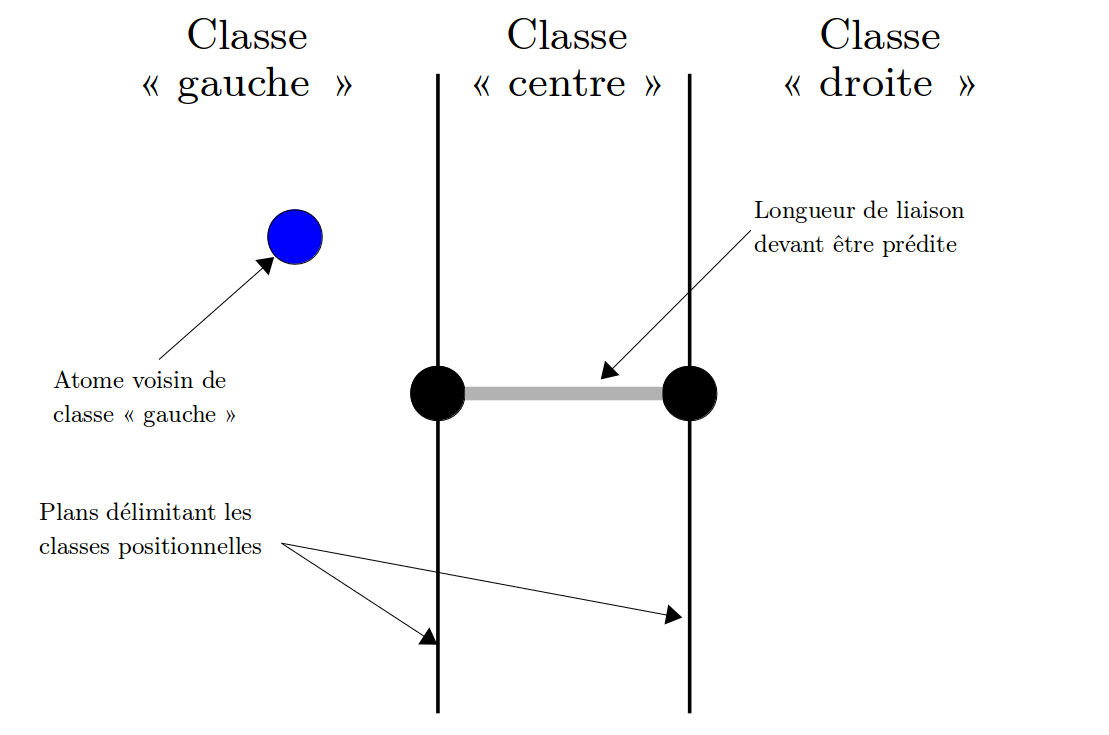
\includegraphics[scale=0.3]{images/classes_pos.png}
	\caption{Classes positionnelles au voisinage d'une liaison covalente}
\end{figure}

\subsection{Distances aux atomes de la liaison}
\par L'influence des atomes au voisinage de la liaison dépend également de leur distance à chacun des deux atomes de la liaison. Plus l'atome voisin est près, plus son influence est forte. C'est pourquoi notre représentation contient également cette information. \\
En fonction des modèles qui l'utilisent, on va éventuellement appliquer une fonction à ces distances, afin de mieux rendre compte de l'influence réelle des atomes au voisinage. Si les réseaux de neurones sont capables d'approximer ces fonctions lors de l'apprentissage, d'autres modèles comme les SVM (REF SVM) ne le sont pas et l'application de ces fonctions est donc nécessaire pour espérer obtenir de bons résultats. Ces fonctions sont les suivantes.\\

\begin{itemize}
\item{Fonction identité : distance brute}
\item{Fonction inverse : influence inversement proportionnelle à la distance, relation d'ordre identique à la réalité chimique.}
\item{Fonction inverse du carré : influence inversement proportionnelle au carré de la distance, relation d'ordre identique à la réalité chimique et rend mieux compte de l'influence réelle des atomes qui suit la loi de Coulomb\footnote{\url{https://fr.wikipedia.org/wiki/Loi_de_Coulomb_(électrostatique)}} en $\frac{1}{d^2}$.}
\end{itemize}

\subsection{Restriction au voisinage le plus proche}
\par L'influence des atomes au voisinage de la liaison étant proportionnelle à l'inverse du carré de leurs distances aux atomes de la liaison, elle décroît rapidement lorsque l'on s'éloigne de la liaison. L'influence des atomes n'étant pas au voisinage direct est ainsi négligeable. Dans le but de ne pas saturer l'entrée des modèles d'information inutile, nous n'enregistrons alors que les informations (classes positionnelles, distances et autres informations non géométriques spécifiques aux différents modèles) concernant les atomes au voisinage proche de la liaison. Formellement, nous enregistrons ces informations pour les atomes dont la distance à au moins un des atomes de la liaison est inférieure à un seuil $\epsilon$  donné.\\

\par Un autre avantage de cette sélection est qu'il existe des molécules aux géométries particulières (repliées) telles que des atomes au voisinage d'une liaison ont très peu d'influence sur sa longueur (ne forment aucune liaison covalente avec les deux atomes de la liaison), et dont la proximité va induire les modèles en erreur. La sélection des atomes au voisinage le plus proche de la liaison avec un seuil $\epsilon$ bien choisi va permettre de résoudre ces problèmes.

\begin{figure}[!h]
	\centering
	
	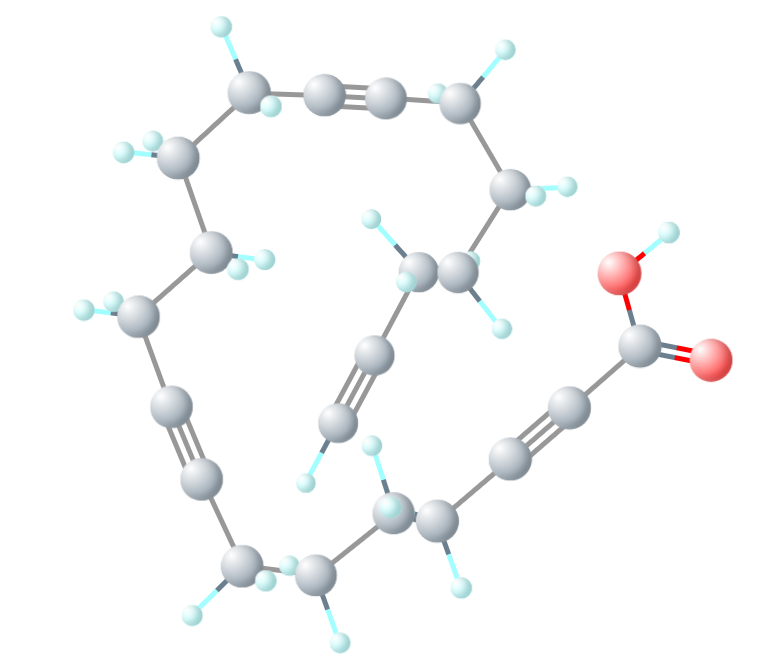
\includegraphics[scale=0.25]{images/mol_repliee.png}
	\caption{Exemple de molécule repliée (CID Pubchem 328310)}
\end{figure}

\chapter{Données}
	\subsubsection{Représentations géométriques}
\par Les modèles que l'on entraîne devant prédire la géométrie des molécules, nous devons leur fournir des données utilisant des représentations synthétisant de la façon la plus simple possible la position des atomes. Nous ne donnons pas les coordonnées brutes aux modèles car ils devraient leur appliquer trop de traitements (REF MAT POS).\\
Les modèles élaborés lors des stages antérieurs utilisaient la représentation géométrique par matrice réduite des distances inter-atomiques (REF MAT. RED. DIST). Elle est basée sur les distances relatives des atomes et possède donc l'avantage d'être indépendante de tout repère absolu. Cependant, il n'est pas possible de reconstruire systématiquement une matrice des positions atomiques à l'issue des prédictions des modèles utilisant cette représentation en sortie. C'est pourquoi nous avons abandonné cette représentation cette année au profit de la matrice des distances à des points fixes (REF MAT PTS FIXES), qui dépend d'un repère absolu mais dont on peut toujours déduire une matrice des positions atomiques.\\

\par Nous avons toutefois entraîné deux modèles de noms DELTA\_DIST\_+H\_03 (resp. DELTA\_DIST\_+H\_04) utilisant comme entrée les deux représentations et comme sortie la représentation par matrice des distances à des points fixes (resp. matrice réduite des distances inter-atomiques). L'entraînement du premier de ces modèles avait pour but de tester si la représentation en repère relatif permettait d'obtenir de meilleurs résultats, et l'entraînement du second avait pour but de vérifier si les mauvaises performances des modèles s'expliquaient par l'utilisation d'une représentation dans un repère absolu. Notons que ce dernier modèle avait uniquement une vocation de test, puisque l'on n'aurait pas été capables de construire la matrice des positons atomiques à l'issue des prédictions, et que l'on n'aurait donc pas pu l'utiliser dans un cas d'utilisation réel.\\

\par Nous avons également utilisé une variante de la représentation par matrice des distances à des points fixes comme entrée de l'un des modèles (DELTA\_DIST\_+H\_02). Dans cette variante, les points fixes de référence sont considérés comme des atomes fictifs et leurs distances relatives sont donc données. Elles avaient initialement été ignorées car elles sont constantes et les réseaux de neurones sont donc théoriquement capables de les \emph{déduire}. Ce modèle permettait de s'assurer que les mauvais résultats ne sont pas dus à cette information manquante.

\subsubsection{Propriétés atomiques}
\par En plus de la géométrie des molécules, nous donnons aux modèles des informations concernant chaque atome et ayant une influence sur la géométrie convergée. Tous les modèles que l'on a entraînés possèdent en entrée la masse atomique de chaque atome, et un des modèles (DELTA\_DIST\_+H\_05) possède également les numéros atomiques. De même que pour les distances entre les points du repère, il s'agit d'une information que les réseaux de neurones sont capables de déduire, nous la donnons pour nous assurer que les mauvais résultats ne sont pas dus à son absence.

\subsubsection{Bruit}
\par L'introduction de bruit dans la géométrie moléculaire convergée et le déplacement des atomes selon les prédictions des modèles pour obtenir la géométrie initiale permet de simuler la prédiction de géométries convergées sur des données réelles (REF INTRODUCT BRUIT). Il nous faut toutefois définir précisément quel type de bruit est introduit, quelles sont les données bruitées et quelle est son intensité.\\

\paragraph{Nature du bruit} Le bruit que l'on introduit est un bruit gaussien de moyenne nulle. Cela semble un choix raisonnable car la symétrie de la distribution permet a priori d'éloigner autant les atomes les uns des autres que de les rapprocher, et le paramètre d'écart-type $\sigma$ permet de contrôler son amplitude avec précision.\\

\paragraph{Données bruitées} Lors des stages antérieurs, le bruit était introduit sur les distances entre les paires d'atomes, au sein de la matrice réduite des distances inter-atomiques. Cela présentait l'avantage de contrôler précisément ses effets. L'utilisation d'une représentation par matrice des distances à des points fixes rend toutefois impossible l'utilisation de cette méthode, car les distances aux points fixes du repère décrivant un point deviendraient incohérentes entre elles. Cela provoquerait la résolution de nombreuses intersections nulles lors de la reconstruction de la matrice des positions atomiques (REF RECONSTRUCT MAT PT FIXES). Pour pallier ce problème, nous introduisons le bruit sur la matrice des positions atomiques avant de calculer la matrice des distances à des points fixes, ce qui garantie sa cohérence mais nous fait perdre une partie du contrôle des effets du bruit. Le bruit étant ajouté aux coordonnées, on peut en effet difficilement vérifier si le déplacement moyen relatif des atomes est nul et on ne peut donc pas savoir si les atomes sont autant éloignés les uns des autres que rapprochés par le bruit.\\

\paragraph{Intensité du bruit} Le déplacement relatif des atomes doit être suffisamment important pour que la tâche d'optimisation de la géométrie moléculaire soit difficile et comparable à des cas d'utilisation réels, mais suffisamment modérée pour que l'on n'inverse pas la position de couples d'atomes, ce qui constituerait une perte d'information trop importante car cela conduirait à tenter d'optimiser des molécules différentes et dans la plupart des cas impossibles selon les lois de la chimie. Un compromis raisonnable semble de déplacer les atomes de 5 pm ($5.10^{-12}$ m) en « moyenne », ou plus précisément d'appliquer un déplacement tel que 68\% des atomes sont déplacés de 5 pm ou moins. Cela revient à utiliser le paramètre d'écart-type $\sigma$ de la loi normale solution de l'équation suivante, exprimant le déplacement d'un atome en pm en fonction de $\sigma$. On note ($x$, $y$, $z$) la position d'un atome dans une géométrie convergée et ($x'$, $y'$, $z'$) sa position après déplacement.

\vspace{0.7cm}

\[
	5 = \sqrt{(x'-x)^2 + (y'-y)^2 + (z'-z)^2}
\]
\[
	5 = \sqrt{\Delta_x^2 + \Delta_y^2 + \Delta_z^2}
\]
\[
	5 = \sqrt{\sigma^2 + \sigma^2 + \sigma^2}
\]
\[
	5 = \sqrt{3\sigma^2}
\]
\[
	\sigma = 2,88675
\]

\vspace{0.7cm}

Certains modèles sont entraînés avec un bruit plus important, tel que 68\% des atomes sont déplacés de 30 pm ou moins. On trouve alors avec la même méthode une valeur pour $\sigma$ de 17,32051. Dans la table des paramètres des modèles en annexe, le bruit faible est noté « + » et le bruit élevé est noté « ++ ».

\subsubsection{Rembourrage des données}



\chapter{Prédiction de longueurs de liaisons convergées}
	\section{Introduction}
		\subsection{Motivation}

Les modèles décrits dans ce chapitre ont pour objectif de prédire la longueur de liaison optimisée entre des atomes partageant une liaison covalente au sein d'une molécule. L'objectif n'est donc pas de résoudre le problème de prédiction d'une géométrie moléculaire convergée complète, mais plutôt d'en résoudre une version locale simplifiée. Chronologiquement, cette classe de modèles est apparue après l'abandon des modèles tentant de prédire la géométrie optimisée complète d'une molécule (REF ABANDON DELTA\_DIST).\\
Puisque l'on résout le problème d'optimisation géométrique entre des couples d'atomes, la question de la façon d'utiliser cette méthode pour optimiser la géométrie complète d'une molécule se pose, nous n'y apportons cependant pas de réponse dans ce chapitre. L'objectif de ces modèles est en effet avant tout de valider notre capacité à effectuer des prédictions d'ordre géométrique de précision suffisante sur certains types de liaisons (REF GENERALISATION). L'élaboration d'une méthode d'optimisation géométrique moléculaire complète basée sur la résolution de sous-problèmes locaux est un problème très complexe, qui fait partie des nouveaux objectifs du projet QuChemPedia (REF PERSPECTIVES MODULES).\\
\par De plus, nous utilisons en entrée des modèles décrits dans ce chapitre des données « parfaites », c'est à dire qu'elles représentent des géométries déjà convergées. Ces données d'entrée ne correspondent donc pas aux données qui seraient utilisées dans un cas d'utilisation réel. L'utilisation de ces données permet cependant d'évaluer la capacité de nos modèles à effectuer des prédictions géométriques lorsque les conditions sont favorables, ce qui représente une première étape dans l'élaboration d'un système permettant de prédire les géométries convergées complètes (REF PERSPECTIVES MODULES).

\subsection{Représentation des données}

\subsubsection{Données en entrée des modèles}
\par Les modèles décrits dans ce chapitre utilisent en entrée la représentation géométrique locale des liaisons covalentes (REF GEOM LOCALE), qui permet de représenter les atomes au voisinage d'une liaison. En plus des informations géométriques, on représente la masse et le numéro atomique de chaque atome au voisinage de la liaison. Le numéro atomique est encodé en \emph{one-hot encoding}, c'est à dire de façon booléenne. La discrétisation des numéros atomiques a pour but de ne pas instaurer de relation d'ordre entre les différents atomes et donc a priori de mieux guider les modèles lors de l'apprentissage. Elle implique toutefois qu'il faut déterminer une limite aux numéros atomiques des atomes acceptés par un modèle. En effet, cet encodage coûte un attribut pour chaque numéro atomique accepté, pour chaque atome au voisinage de la liaison. Afin de travailler sur des modèles de taille raisonnable, ils acceptent les atomes de numéros atomiques inférieurs ou égaux à celui du fluor, ce qui correspond à neuf attributs encodant le numéro atomique pour chaque atome du voisinage.
\par De même la classe positionnelle (REF CLASSE POS) de chaque atome par rapport à la liaison est représenté en \emph{one-hot encoding}, afin de ne pas représenter cette information sur un ensemble possédant une relation d'ordre.\\

\par Le tableau suivant présente le nombre d'attributs utilisés pour représenter chaque atome au voisinage d'une liaison.

\begin{figure}[!h]
	\centering
	
	\begin{tabular}{|c|c|c|c|c|}
		\hline
		\textbf{Classe positionnelle} & \textbf{Distances} & \textbf{Masse atomique} & \textbf{Numéro atomique} & \textbf{Total}\\ \hline
		3 & 2 & 1 & 9 & 15\\ \hline
	\end{tabular}
	\caption{Quantité d'attributs représentant chaque atome au voisinage d'une liaison}
\end{figure}

\subsubsection{Homogénéisation de la taille des entrées}
\par Les molécules possédant un nombre variable d'atomes et l'entrée des modèles étant de taille fixe, nous effectuons une procédure de \emph{padding}\footnote{Rembourrage} des données. Cela signifie que l'entrée des modèles est découpée en blocs, représentant chacun un atome au voisinage de la liaison. La taille des blocs dépend des attributs représentant chaque atome, et le nombre de blocs définit le nombre maximal d'atomes au voisinage des liaisons que les modèles peuvent traiter. Nous déduisons cette information de la taille des molécules que l'on choisit d'accepter en entrée des modèles. La grande majorité des molécules étant de taille inférieure à 60 (VOIR DONNEES DISTRIB TAILLES) et les deux atomes composant la liaison n'apparaissant pas dans les entrées, nous choisissons de limiter le voisinage de la liaison à 58 atomes.\\
\par La représentation d'une liaison en entrée des modèles est donc composée de 58 blocs de 15 attributs, soit 870 valeurs. Lorsqu'une liaison possède moins de 58 voisins, les blocs correspondant aux atomes non définis valent zéro.

\subsubsection{Représentation d'une liaison en entrée d'un modèle}

\par Nous détaillons la représentation en entrée d'un modèle prédictif de la liaison imaginaire utilisée comme exemple en (REF REPR LOCALE). On considère que l'atome a$_3$ est un atome d'azote et que l'atome a$_4$ est un atome d'oxygène.

\vspace{0.5cm}

\begin{figure}[!h]
	\centering
	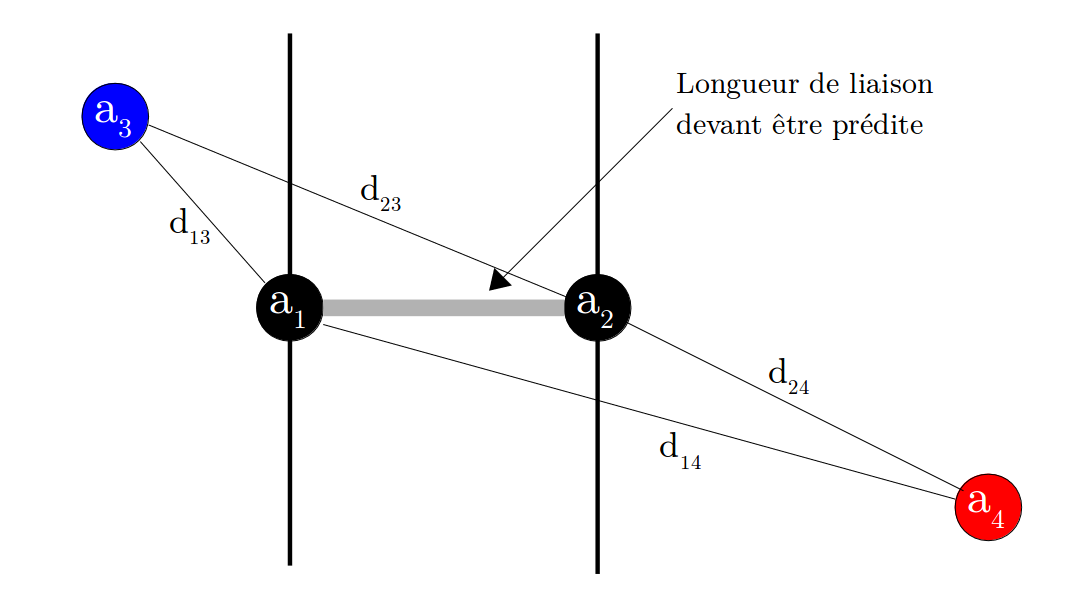
\includegraphics[scale=0.3]{images/classes_pos_4.png}
	\caption{Représentation schématique d'une liaison imaginaire}
\end{figure}

\par L'entrée correspondant à la liaison représentée ci-dessus est donnée dans le tableau suivant.

\begin{figure}[!h]
	\centering


	\begin{tabular}{|c|c|c|c|c|c|c|c|c|c|c|c|c|c|c|}
		\hline
		\multicolumn{3}{|c|}{\textbf{Classe pos.}} & \multicolumn{2}{|c|}{\textbf{Distances}} & \textbf{Masse atomique} & \multicolumn{9}{|c|}{\textbf{Numéro atomique}} \\
		\textbf{g?} & \textbf{c?} & \textbf{d?} & \multicolumn{2}{|c|}{}& & \textbf{H?} & \textbf{He?} & \textbf{Li?} & \textbf{Be?} & \textbf{B? }& \textbf{C?} & \textbf{N?} & \textbf{O?} & \textbf{F?} \\ \hline
		1 & 0 & 0 & $d_{13}$ & $d_{23}$ & 14,007 & 0 & 0 & 0 & 0 & 0 & 0 & 1 & 0 & 0 \\ \hline
		0 & 0 & 1 & $d_{14}$ & $d_{24}$ & 15,999 & 0 & 0 & 0 & 0 & 0 & 0 & 0 & 1 & 0 \\ \hline
		0 & 0 & 0 & 0 & 0 & 0 & 0 & 0 & 0 & 0 & 0 & 0 & 0 & 0 & 0 \\ \hline
		\rot{... } & \rot{... } & \rot{... } & \rot{... } & \rot{... } & \rot{... } & \rot{... } & \rot{... } & \rot{... } & \rot{... } & \rot{... } & \rot{... } & \rot{... } & \rot{... } & \rot{... }  \\ \hline 
		0 & 0 & 0 & 0 & 0 & 0 & 0 & 0 & 0 & 0 & 0 & 0 & 0 & 0 & 0 \\ \hline
	\end{tabular}

	\caption{Représentation des données d'une liaison en entrée d'un modèle prédictif}
\end{figure}



\subsection{Méthodologie}

\subsubsection{Précision requise}
\par Les modèles décrits dans ce chapitre travaillent sur des données « parfaites », c'est à dire qu'il prédisent des longueurs de liaisons dans des molécules dont la géométrie a déjà été optimisée. Cela nous permet de confirmer notre capacité à effectuer des prédictions d'ordre géométrique, mais pas de nous assurer que les modèles pourront effectuer de bonnes prédictions sur des données non optimisées issues de mesures ou de résultats théoriques. L'entraînement de modèles travaillant sur des données imparfaites fera l'objet de la suite du projet QuChemPedia (REF PERSPECTIVES). Pour pouvoir espérer obtenir de bonnes prédictions sur des données non optimisées, il faut obtenir de très bons résultats sur des données optimisées, comme on le montre en REF GENERALISATION.

\par La précision que l'on peut espérer atteindre avec les données sur lesquelles les modèles s'entraînent (REF PUBCHEM) est de l'ordre du picomètre (pm), soit $10^{-12}$ m. Cette précision dépend des fonctions choisies lors de l'optimisation géométrique quantique des molécules (REF OPTI DFT). Les modèles effectuant des prédictions dont l'erreur est inférieure à 1 pm confirmeront donc notre capacité à effectuer des prédictions d'ordre géométrique de précision suffisante.

\subsubsection{Classes de modèles}
\par Nous tentons de prédire les longueurs de liaisons entre plusieurs couples d'atomes, en entraînant un modèle par couple d'atomes formant une liaison. Les liaisons carbone-carbone ne seront alors pas prédites par le même modèle que les liaisons carbone-hydrogène. Cette séparation en sous-problèmes segmentés a pour objectif d'évaluer la précision que peuvent atteindre les modèles sur les problèmes les plus simples que l'on peut leur donner. L'évaluation de leur précision sur des problèmes plus complexes fait partie des futurs objectifs (REF	MODULES PLUSIEURS LIAISONS). La prédiction des longueurs de liaisons d'un unique couple donné d'atomes par modèle n'en fait toutefois pas un problème trivial, car elles peuvent sensiblement varier en fonction des atomes impliqués (REF DISTRIB LONGUEURS). Si les liaisons oxygène-hydrogène ont une taille variant en général entre 97 pm et 102 pm soit avec une amplitude de 5 pm, la taille des liaisons carbone-carbone varie entre 120 pm et 160 pm, ce qui représente une amplitude de 40 pm. \\
\par L'entraînement des modèles est un processus qui prend un temps non négligeable (REF CONTRAINTES MATERIELLES). Pour cette raison, nous n'entraînons pas tous les modèles sur un grand nombre d'exemples et nous définissons deux classes de modèles ayant des objectifs différents. \\
\par La première classe de modèles a un objectif d'expérimentation. Les modèles sont entraînés sur un nombre relativement faible d'exemples différents sur 150 époques (REF DEF EPOCH), ce qui représente environ 2h de préparation de données et 6h d'entraînement avec le matériel disponible. Ces modèles sont entraînés dans le but d'expérimenter de nouveaux traitements des données d'entrée ou de nouveaux paramètres. Ils ont pour objectif de discriminer la qualité de ces entrées et paramètres, c'est pourquoi ils travaillent sur la prédiction difficile des distances de liaisons carbone-carbone. Ces modèles sont décrits en REF PRED C.	\\
\par La seconde classe de modèles a un objectif de validation des paramètres performants issus de l'entraînement des modèles de la première classe, ainsi qu'un objectif de généralisation des méthodes à différents types de liaisons. Ces modèles s'entraînent donc sur plus d'exemples et sur plusieurs liaisons différentes (carbone-carbone, carbone-hydrogène et oxygène-hydrogène). L'entraînement des trois modèles de cette classe pour un ensemble d'entrées et de paramètres donné prend environ deux jours. Ces modèles sont décrits en REF GENERALISATION.

\subsection{Nomenclature}
\par Afin d'y faire référence simplement, nous nommons les différents modèles que l'on entraîne. Tous les modèles décrits dans ce chapitre ont pour préfixe \emph{DIST\_REL}, issu de leur vocation à prédire la distance relative entre les atomes d'une liaison, et pour suffixe le numéro chronologique de leur entraînement au sein de leur classe.\\
Les modèles de la première classe (resp. seconde) ont pour préfixe \emph{DIST\_REL\_C} (resp. \emph{DIST\_REL\_XY}, où X et Y désignent les symboles des éléments formant la liaison prédite). La différence de nomenclature entre les deux classes et notamment entre les modèles \emph{DIST\_REL\_C} et \emph{DIST\_REL\_CC} est discutable, mais a pour avantage de faire apparaître simplement la distinction.\\
Enfin, les modèles prédictifs n'étant pas des réseaux de neurones artificiels font apparaître leur type dans leur nom.

	\section{Prédiction de longueurs de liaisons carbone-carbone}
		\subsection{Modèle naïf}

\subsection{Restriction au voisinage le plus proche}

\subsection{Application de fonctions aux distances}

\subsection{Réduction de la largeur du réseau}

\subsection{Recherche par quadrillage des paramètres du modèle naïf}


	\section{Généralisation de la méthode à d'autres liaisons}
		\label{dist_rel_generalisation}

\par Les modèles décrits dans cette section appartiennent à la seconde classe (\ref{dist_rel_classes_explication}). Leur objectif est de valider les paramètres et les entrées des modèles de la première classe, et de généraliser la méthode à plusieurs liaisons différentes. Pour cela, nous préparons des jeux de données de grandes tailles, et nous entraînons les modèles sur 300 époques, pour les liaisons carbone-carbone, carbone-hydrogène et oxygène-hydrogène. Les tailles des jeux de données pour chacun des modèles sont données dans le tableau \ref{t_tailles_dist_rel_xy}. Si seulement une partie des molécules est explorée pour générer les jeux de données concernant les liaisons carbone-carbone et carbone-hydrogène du fait de leur grande représentation dans les données, toutes les molécules sont explorées pour générer les exemples concernant les liaisons oxygène-hydrogène, qui sont moins nombreuses dans les molécules de notre jeu de données (\ref{donnees_bases}).
\par Notons que les modèles \emph{DIST\_REL\_C} et \emph{DIST\_REL\_CC} prédisent les mêmes longueurs de liaisons (carbone-carbone), la différence entre les deux étant la taille des jeux de données utilisés et la durée d'entraînement.

\begin{table}
	\centering
		\begin{tabular}{|l|l|l|l|}
			\hline
			\textbf{Jeu} & \textbf{Modèles \emph{DIST\_REL\_CC}} & \textbf{Modèles \emph{DIST\_REL\_CH}} & \textbf{Modèles \emph{DIST\_REL\_OH}} \\ \hline
			Entraînement & 5541305 & 3636608 & 1293551 \\ \hline
			Test & 1106823 & 1158251 & 143588 \\ \hline
		\end{tabular}

	\caption{Tailles des jeux de données des modèles \emph{DIST\_REL\_XY}}
	\label{t_tailles_dist_rel_xy}
\end{table}

Les paramètres d'entraînement communs utilisés par tous les modèles \emph{DIST\_REL\_XY} sont donnés dans la tableau \ref{tparams_dist_rel_xy}.

\begin{table}
	\centering
	\begin{tabular}{|l|l|}
		\hline
		\textbf{Paramètre} & \textbf{Valeur} \\ \hline
		Taille de lot (\emph{batch size}) & 10000 \\ \hline
		Epsilon (Adam) & 0.001 \\ \hline
		Initialisation des poids (\emph{stddev\_init}) & 0.001 \\ \hline
		Fonction d'activation couches cachées & elu \\ \hline
		Fonction d'activation couche de sortie & linéaire \\ \hline
		Abandon (\emph{dropout}) & 0.98 \\ \hline
		Dégradation des coefficients (\emph{weight decay}) & 0.001 \\ \hline
	\end{tabular}

	\caption{Paramètres d'entraînement des modèles \emph{DIST\_REL\_XY}}
	\label{tparams_dist_rel_xy}
\end{table}

\subsection{Modèles naïfs}

\label{dist_rel_xy_naif}

Les trois modèles naïfs sont entraînés avec les mêmes paramètres et le même traitement des données d'entrée que leur modèle équivalent de la première classe (\ref{dist_rel_c_naif}), c'est à dire qu'aucune restriction au voisinage le plus proche de la liaison n'est appliquée, et qu'aucune fonction n'est appliquée aux distances.

\subsubsection{Analyse statistique des erreurs}
\par Dans le tableau \ref{t_stats_dist_rel_xy_01}, nous présentons les valeurs des différentes métriques permettant d'évaluer les erreurs pour les modèles prédisant chaque type de liaison. Afin de comparer les performances du modèle prédisant les longueurs de liaisons carbone-carbone avec le modèle de la première classe équivalent, nous rappelons également la valeur des métriques du modèle \emph{DIST\_REL\_C\_01}.
\par L'entraînement sur un nombre plus élevé d'exemples fait apparaître un gain non négligeable pour la prédiction de longueurs de liaisons entre des atomes de carbone. La moyenne passe en effet en dessous de la barre cible de 1 pm. L'écart-type est cependant toujours au dessus du pm, même si sa valeur est peu interprétable du fait de la distribution non gaussienne des erreurs.
\par La prédiction des autres types de liaisons montre de très bons résultats, la plupart des métriques étant à des valeurs proches du dixième de picomètre. Les erreurs maximales ont toutefois des valeurs relativement élevées, notamment dans le cas de la prédiction des liaisons carbone-hydrogène.

\begin{table}
	\centering
	\begin{tabular}{|l|r|r|r|r|}
		\hline
		\textbf{Métrique}& \textbf{\emph{D\_REL\_C\_01}} &\textbf{\emph{D\_REL\_CC\_01}} & \textbf{\emph{D\_REL\_CH\_01}} & \textbf{\emph{D\_REL\_OH\_01}}\\ \hline
		Moyenne & 1,3301 & 0,8334 & 0,1753 & 0,1947\\ \hline
		Médiane & 0,6881 & 0,4604 & 0,1132 & 0,1153\\ \hline
		Écart-type & 1,9810 & 1,2066 & 0,1961 & 0,2519 \\ \hline
		Minimum & 0,0000 & 0,0000 & 0.0000 & 0.0000\\ \hline
		Maximum & 28,7268 & 30,1138 & 22,1473 & 7,2530\\ \hline
		Erreur rel. & 0,9126\% & 0,5709\% & 0,1599\% & 0.1986\%\\ \hline
	\end{tabular}
	
	\caption{Analyse statistique des erreurs des modèles (en pm)}
	\label{t_stats_dist_rel_xy_01}
\end{table}

\subsubsection{Représentation graphique des résultats}

\par La distribution des erreurs des modèles prédisant les longueurs de liaisons entre les atomes de carbone et d'hydrogène et entre les atomes d'hydrogène et d'oxygène montre que les plus grosses erreurs sont marginales en représentation (figures \ref{fdistrib_err_dist_rel_ch_01} et \ref{fdistrib_err_dist_rel_oh_01}). \\


\begin{figure}
	\centering
	
	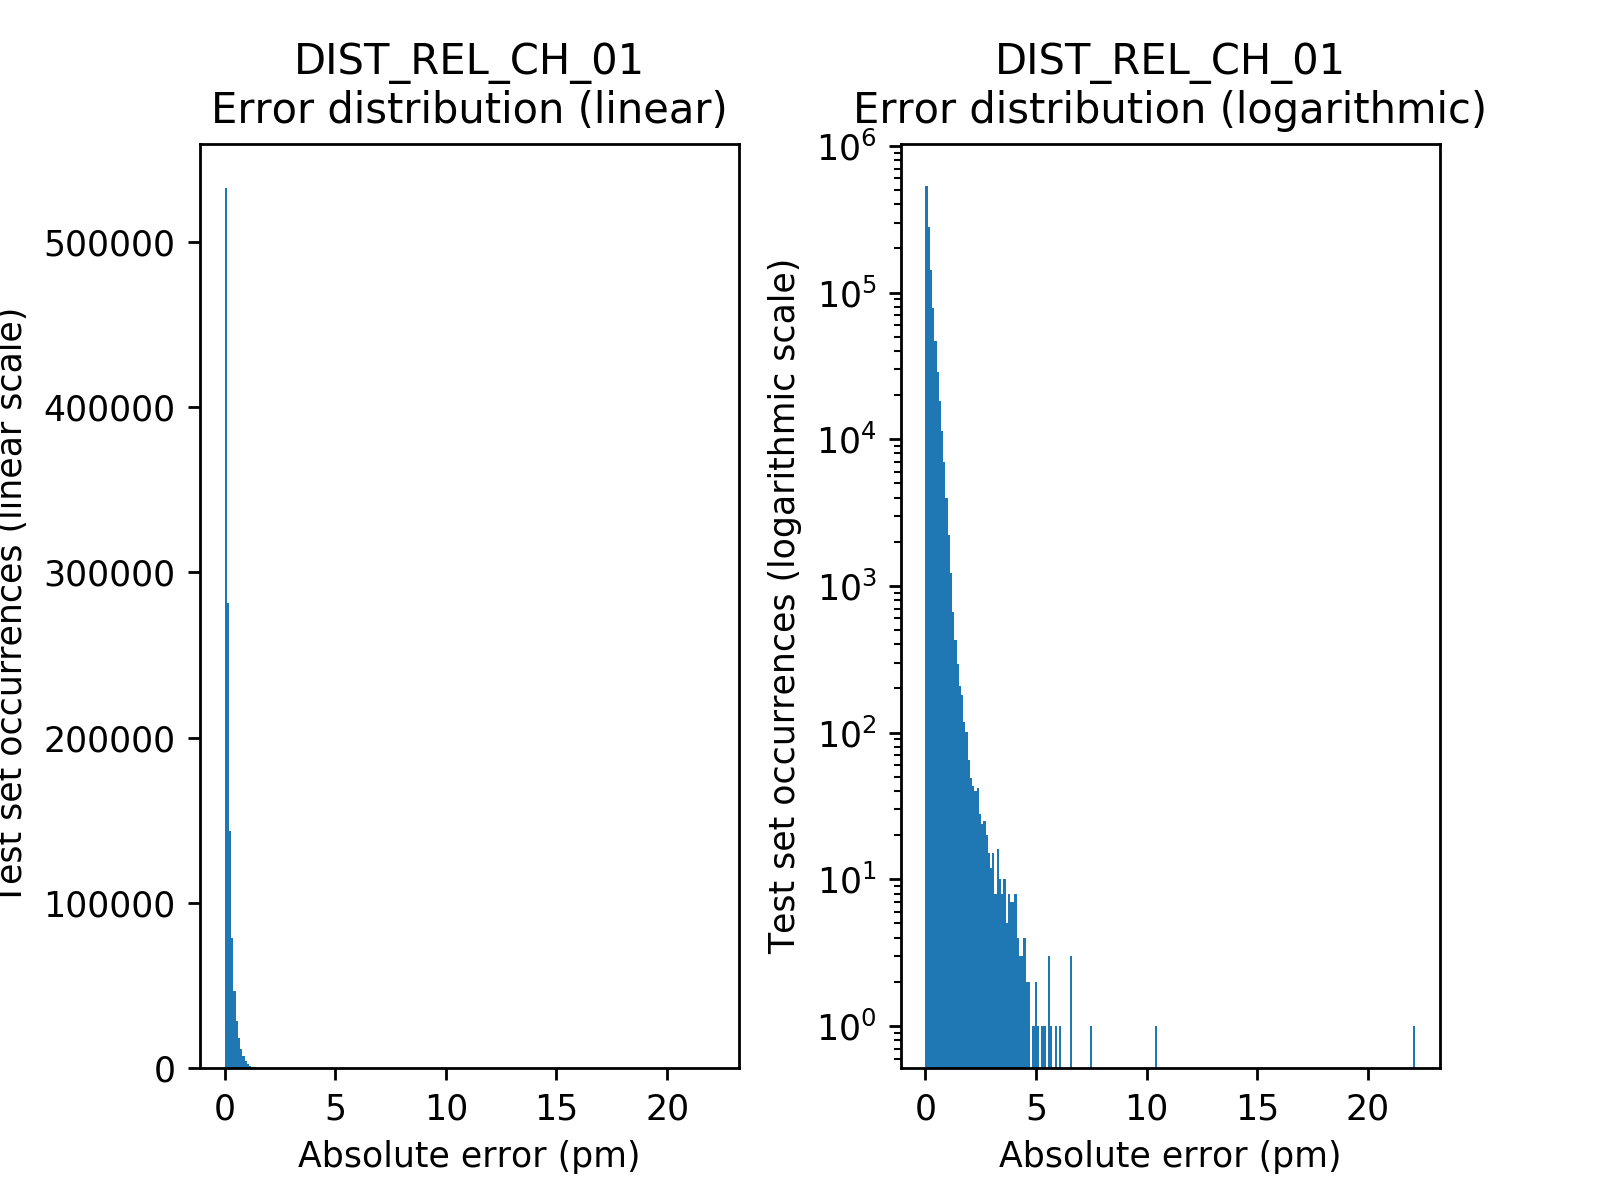
\includegraphics[scale=0.7]{../figures/DIST_REL_CH_01/DIST_REL_CH_01_distrib_rmse_val.png}	
	
	\caption{Distribution des erreurs du modèle \emph{DIST\_REL\_CH\_01}}
	\label{fdistrib_err_dist_rel_ch_01}

\end{figure}
\begin{figure}
	\centering
	
	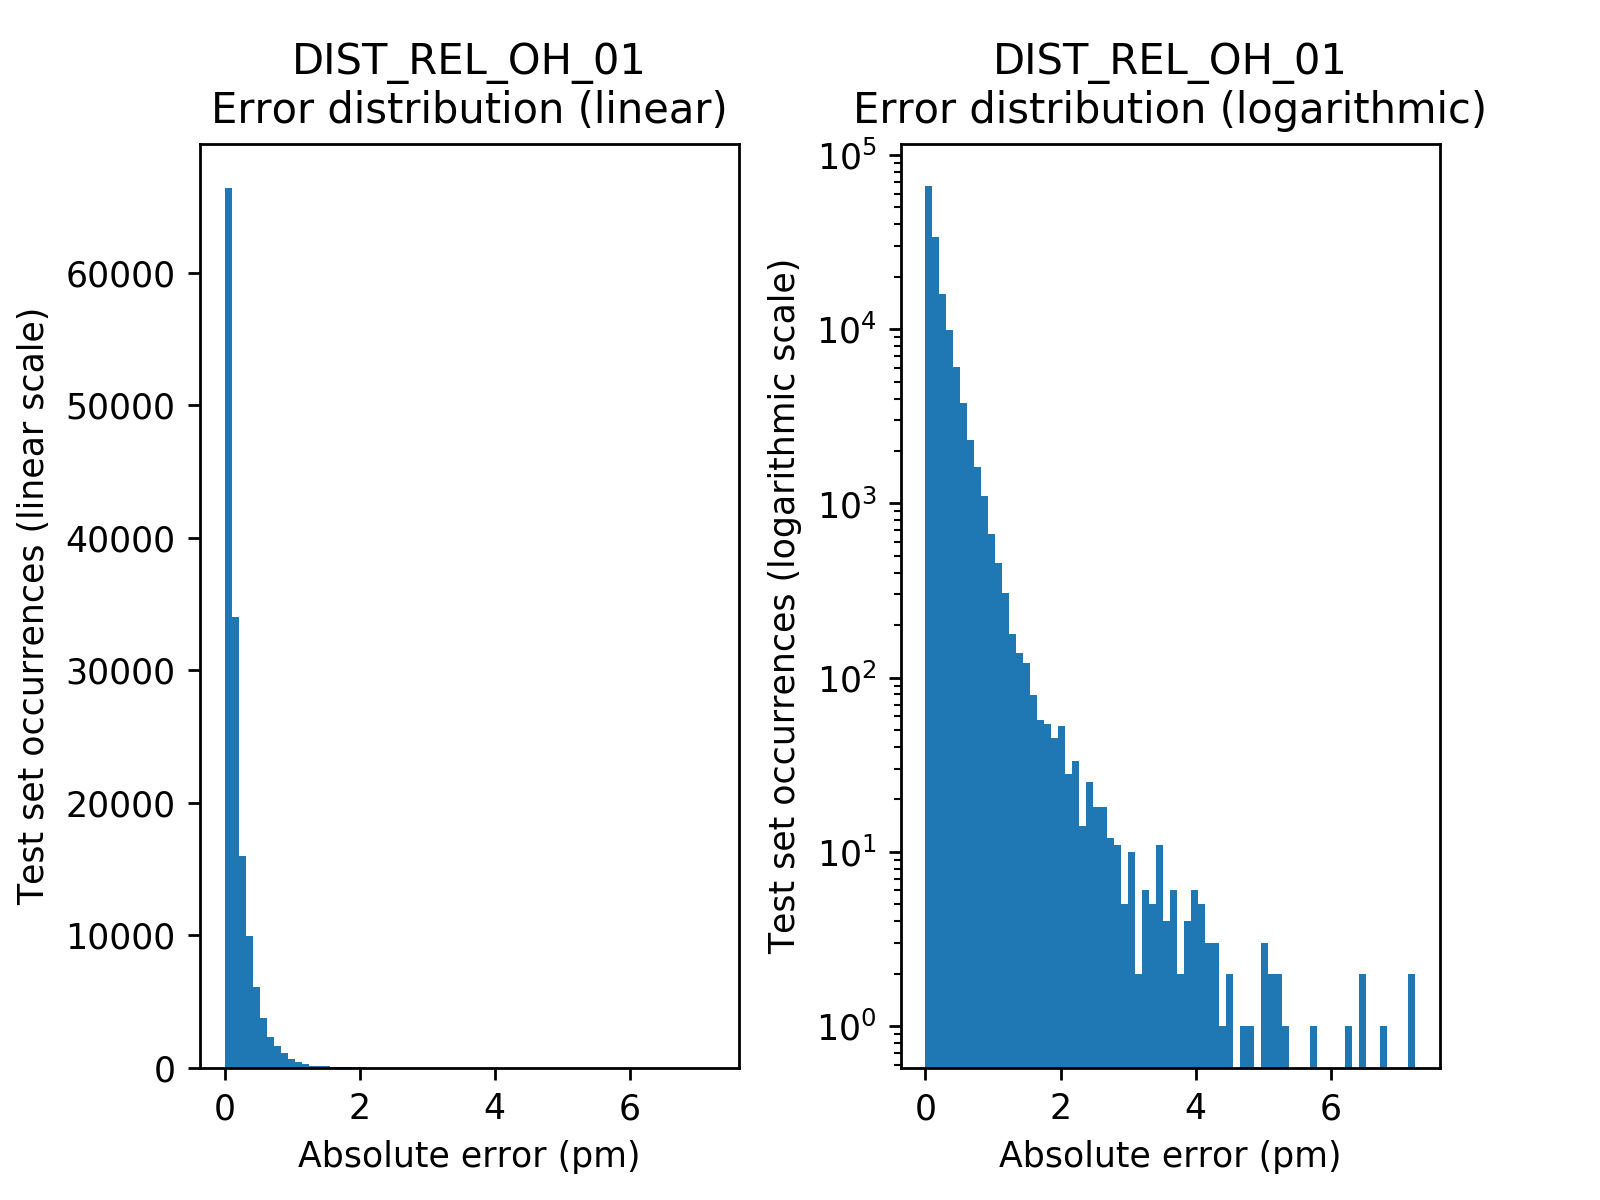
\includegraphics[scale=0.7]{../figures/DIST_REL_OH_01/DIST_REL_OH_01_distrib_rmse_val.png}	
	
	\caption{Distribution des erreurs du modèle \emph{DIST\_REL\_OH\_01}}
	\label{fdistrib_err_dist_rel_oh_01}

\end{figure}

\par La représentation graphique des erreurs relatives (figure \ref{fdistrib_err_rel_dist_rel_oh_01}) et des prédictions en fonction des cibles (figure \ref{fpreds_targets_dist_rel_oh_01}) montre un phénomène intéressant pour le modèle prédisant les longueurs de liaisons entre les atomes d'oxygène et d'hydrogène. La représentation des longueurs de liaisons OH chutant brusquement en deçà de 97 pm, le modèle s'adapte à cette particularité en ne prédisant jamais des valeurs inférieures à 97 pm.

\begin{figure}
	\centering
	
	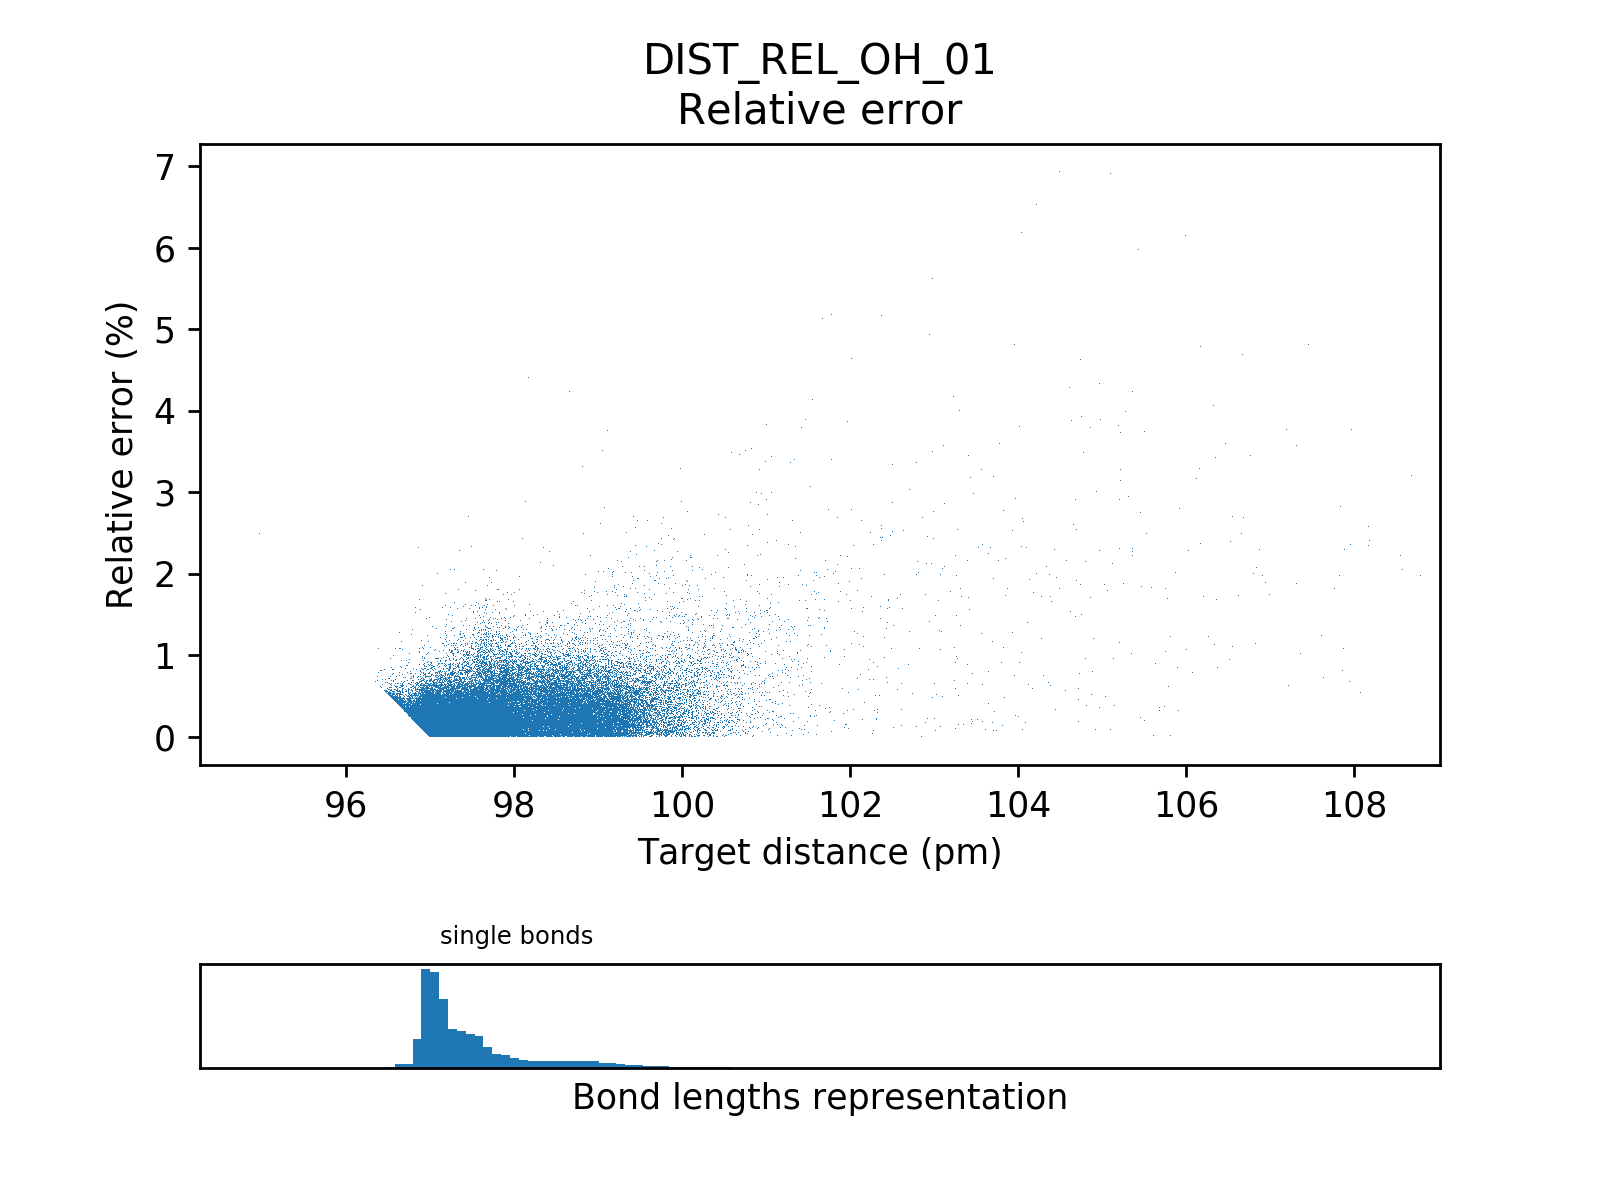
\includegraphics[scale=0.7]{../figures/DIST_REL_OH_01/DIST_REL_OH_01_distrib_rmse_dist.png}	
	
	\caption{Erreur en fonction des cibles pour le modèle \emph{DIST\_REL\_OH\_01}}
	\label{fdistrib_err_rel_dist_rel_oh_01}
	\end{figure}
	
\begin{figure}
	\centering
	
	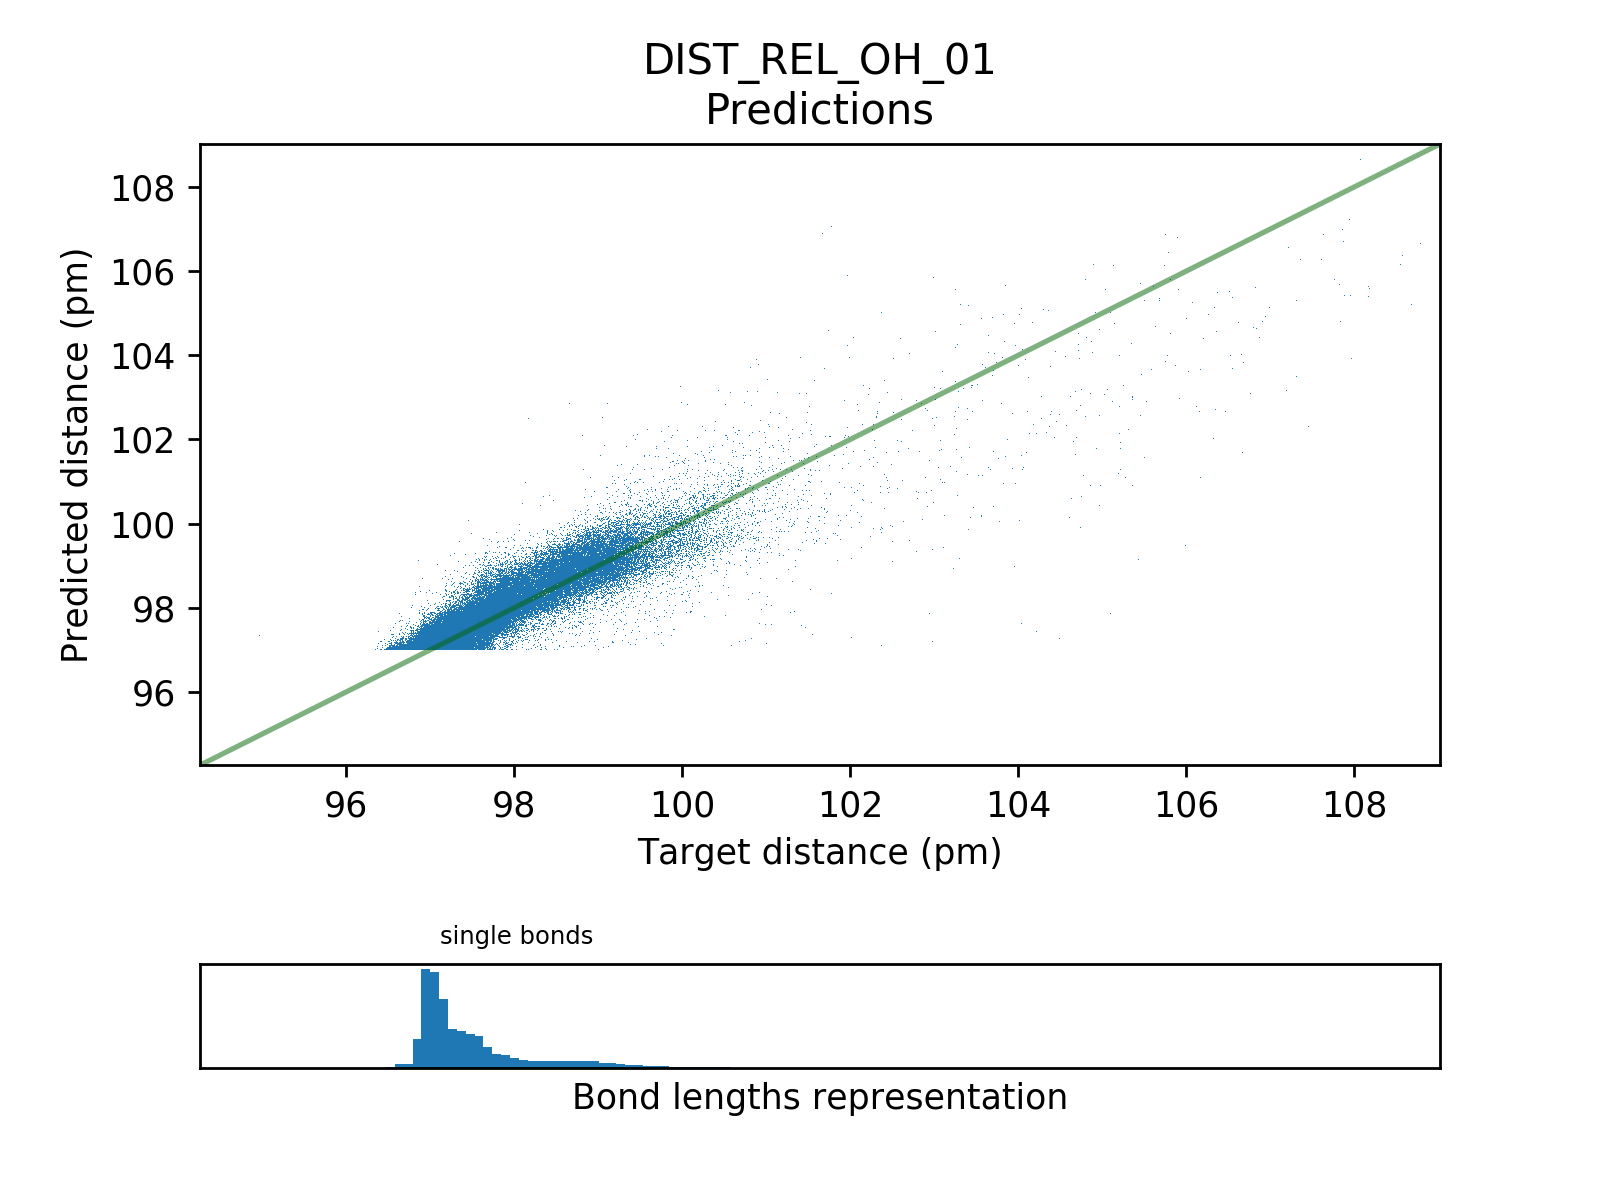
\includegraphics[scale=0.7]{../figures/DIST_REL_OH_01/DIST_REL_OH_01_preds_targets.png}	
	
	\caption{Prédictions en fonction des cibles pour le modèle \emph{DIST\_REL\_OH\_01}}
	\label{fpreds_targets_dist_rel_oh_01}

\end{figure}

\par Enfin, la représentation graphique des erreurs relatives (figure \ref{fdistrib_err_rel_dist_rel_ch_01}) et des prédictions (figure \ref{fpreds_targets_dist_rel_ch_01}) du modèle prédisant les longueurs de liaison carbone-hydrogène montre que les très bons résultats du modèle s'expliquent en partie par la faible dispersion des longueurs cibles.\\
Les représentations graphiques concernant le modèle prédisant les liaisons carbone-carbone étant très semblables à celles du modèle \emph{DIST\_REL\_C\_01}, elles sont uniquement visibles en annexe \ref{annexes_plot_dist_rel_xy}.

\begin{figure}
	\centering
	
	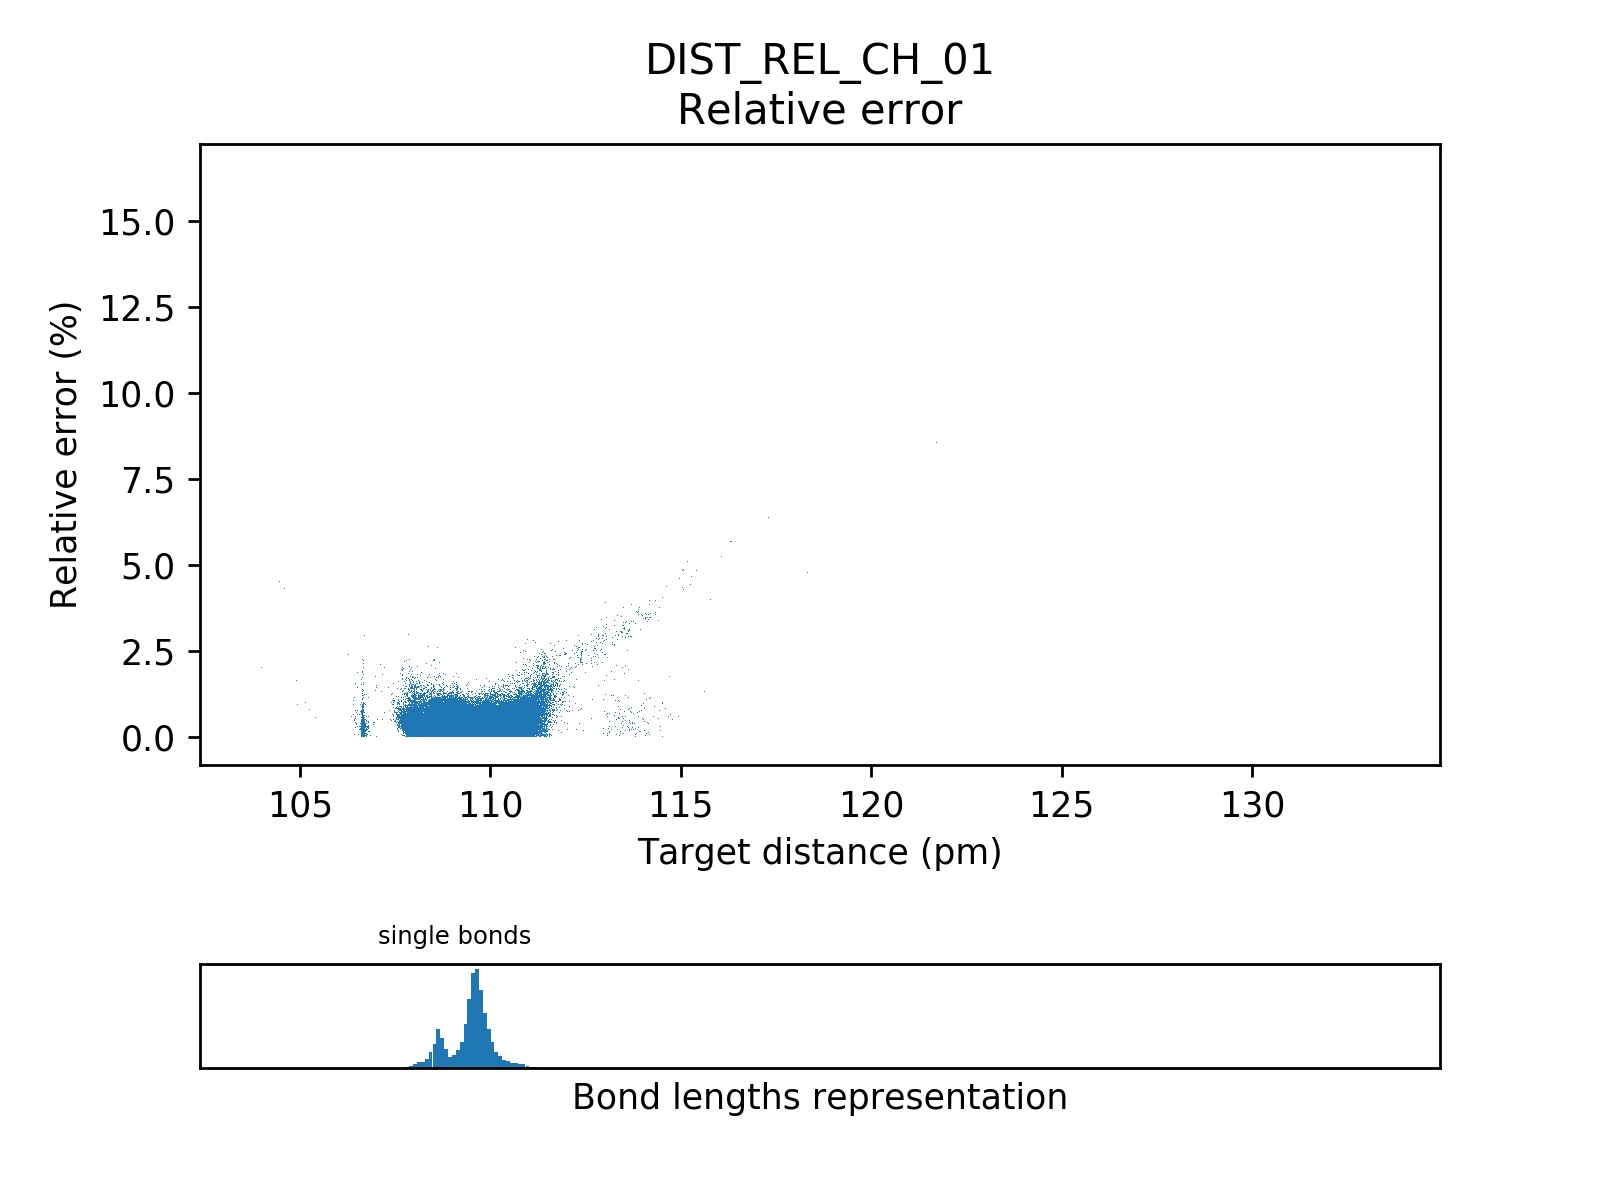
\includegraphics[scale=0.7]{../figures/DIST_REL_CH_01/DIST_REL_CH_01_distrib_rmse_dist.png}	
	
	\caption{Erreur en fonction des cibles pour le modèle \emph{DIST\_REL\_CH\_01}}
	\label{fdistrib_err_rel_dist_rel_ch_01}
	\end{figure}
	
\begin{figure}
	\centering
	
	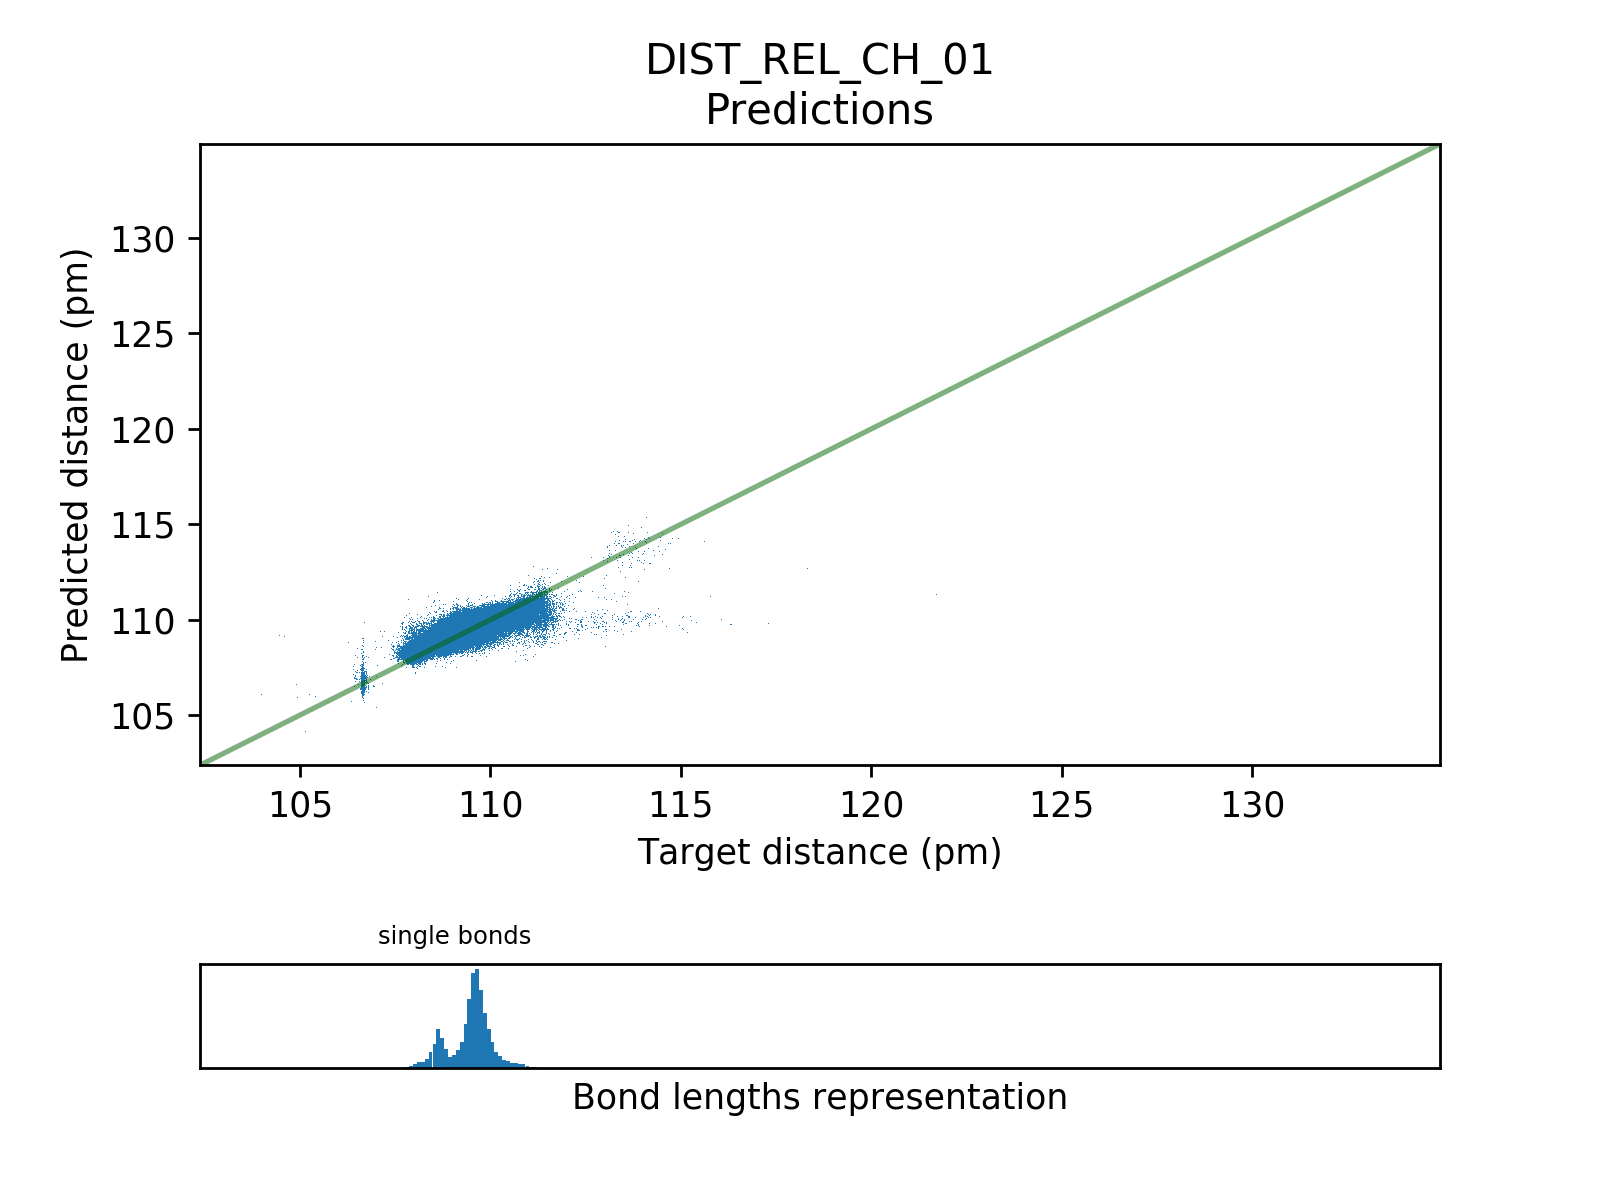
\includegraphics[scale=0.7]{../figures/DIST_REL_CH_01/DIST_REL_CH_01_preds_targets.png}	
	
	\caption{Prédictions en fonction des cibles pour le modèle \emph{DIST\_REL\_CH\_01}}
	\label{fpreds_targets_dist_rel_ch_01}

\end{figure}

\subsection{Restriction au voisinage le plus proche}

\label{dist_rel_xy_restrict}

\par Les modèles décrits dans cette partie sont les modèles de la seconde classe équivalents aux modèles décrits en \ref{dist_rel_c_restriction}.

\subsubsection{Analyse statistique des erreurs}
\par Le tableau \ref{tstats_dist_rel_xy_02} donne les valeurs des différentes métriques évaluant les erreurs des modèles. Comme attendu, la restriction aux atomes au plus proche voisinage améliore en général les performances des modèles, notamment dans le cas du modèle prédisant les longueurs de liaisons entre des atomes de carbone. Les prédictions concernant les longueurs de liaisons entre des atomes d'hydrogène et d'oxygène sont également améliorées d'un facteur moindre. Toutefois, les prédictions des longueurs de liaisons entre des atomes de carbone et d'hydrogène sont impactées négativement par cette nouvelle approche, même si l'erreur maximale est diminuée d'un facteur trois.


\begin{table}
	\centering
	\begin{tabular}{|l|r|r|r|}
		\hline
		\textbf{Métrique}& \textbf{\emph{DIST\_REL\_CC\_02}} & \textbf{\emph{DIST\_REL\_CH\_02}} & \textbf{\emph{DIST\_REL\_OH\_02}}\\ \hline
		Moyenne & 0,3416 & 0,2390 & 0,1519\\ \hline
		Médiane &  0.2667 & 0.2010 &  0,1044\\ \hline
		Écart-type & 0,3373 & 0,1884 & 0,1648 \\ \hline
		Minimum & 0,0000 & 0,0000 & 0.0000\\ \hline
		Maximum & 26.2167 & 6,2905 & 4,7264 \\ \hline
		Erreur rel. & 0,2295\% & 0,2184\% & 0,1552\%\\ \hline
	\end{tabular}
	
	\caption{Analyse statistique des erreurs des modèles (en pm)}
	\label{tstats_dist_rel_xy_02}
\end{table}

\subsubsection{Analyse graphique des résultats}

\par Les représentations graphiques des erreurs (figures \ref{fdistrib_err_dist_rel_cc_02} et \ref{fdistrib_err_rel_dist_rel_cc_02}) et des prédictions (figure \ref{fpreds_targets_dist_rel_cc_02}) du modèle prédisant les longueurs de liaisons entre des atomes de carbone font nettement apparaître la diminution des erreurs importantes et la continuité des prédictions entre les différents types de liaisons.


\begin{figure}
	\centering
	
	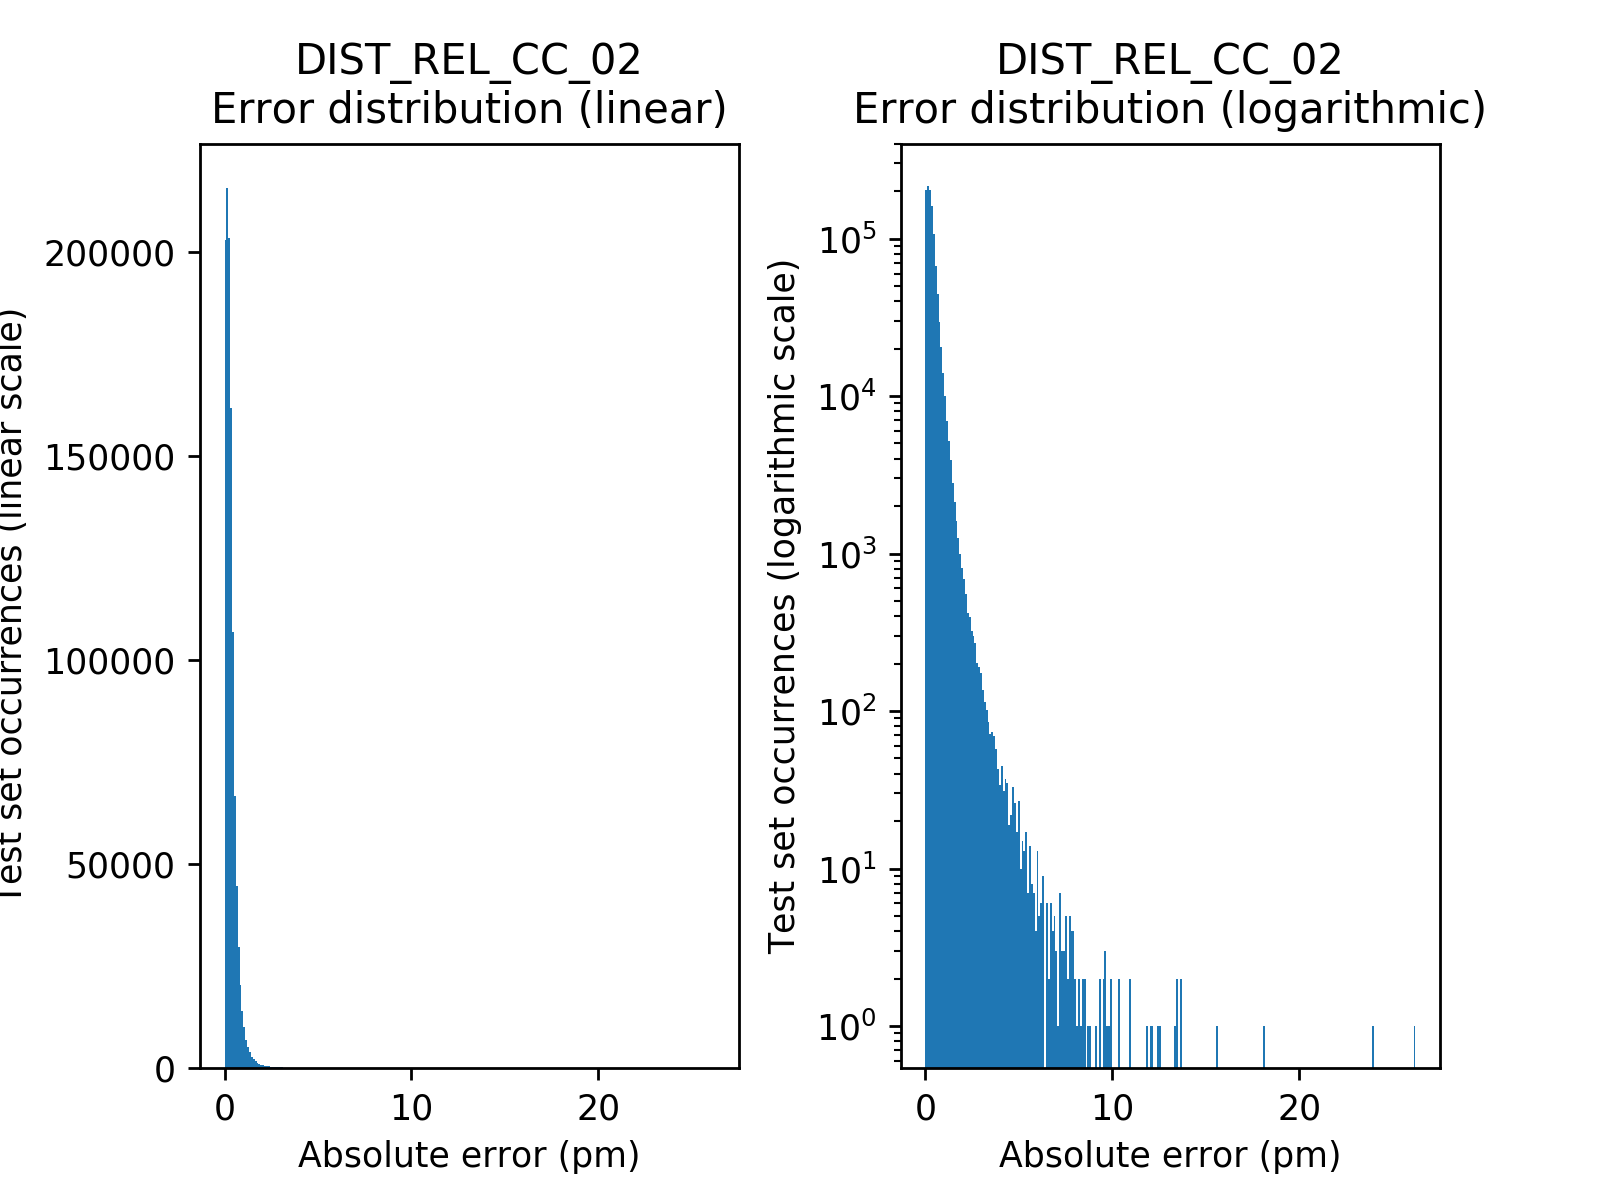
\includegraphics[scale=0.8]{../figures/DIST_REL_CC_02/DIST_REL_CC_02_distrib_rmse_val.png}	
	
	\caption{Distribution des erreurs du modèle \emph{DIST\_REL\_CC\_02}}
	\label{fdistrib_err_dist_rel_cc_02}
\end{figure}
\begin{figure}
	\centering
	
	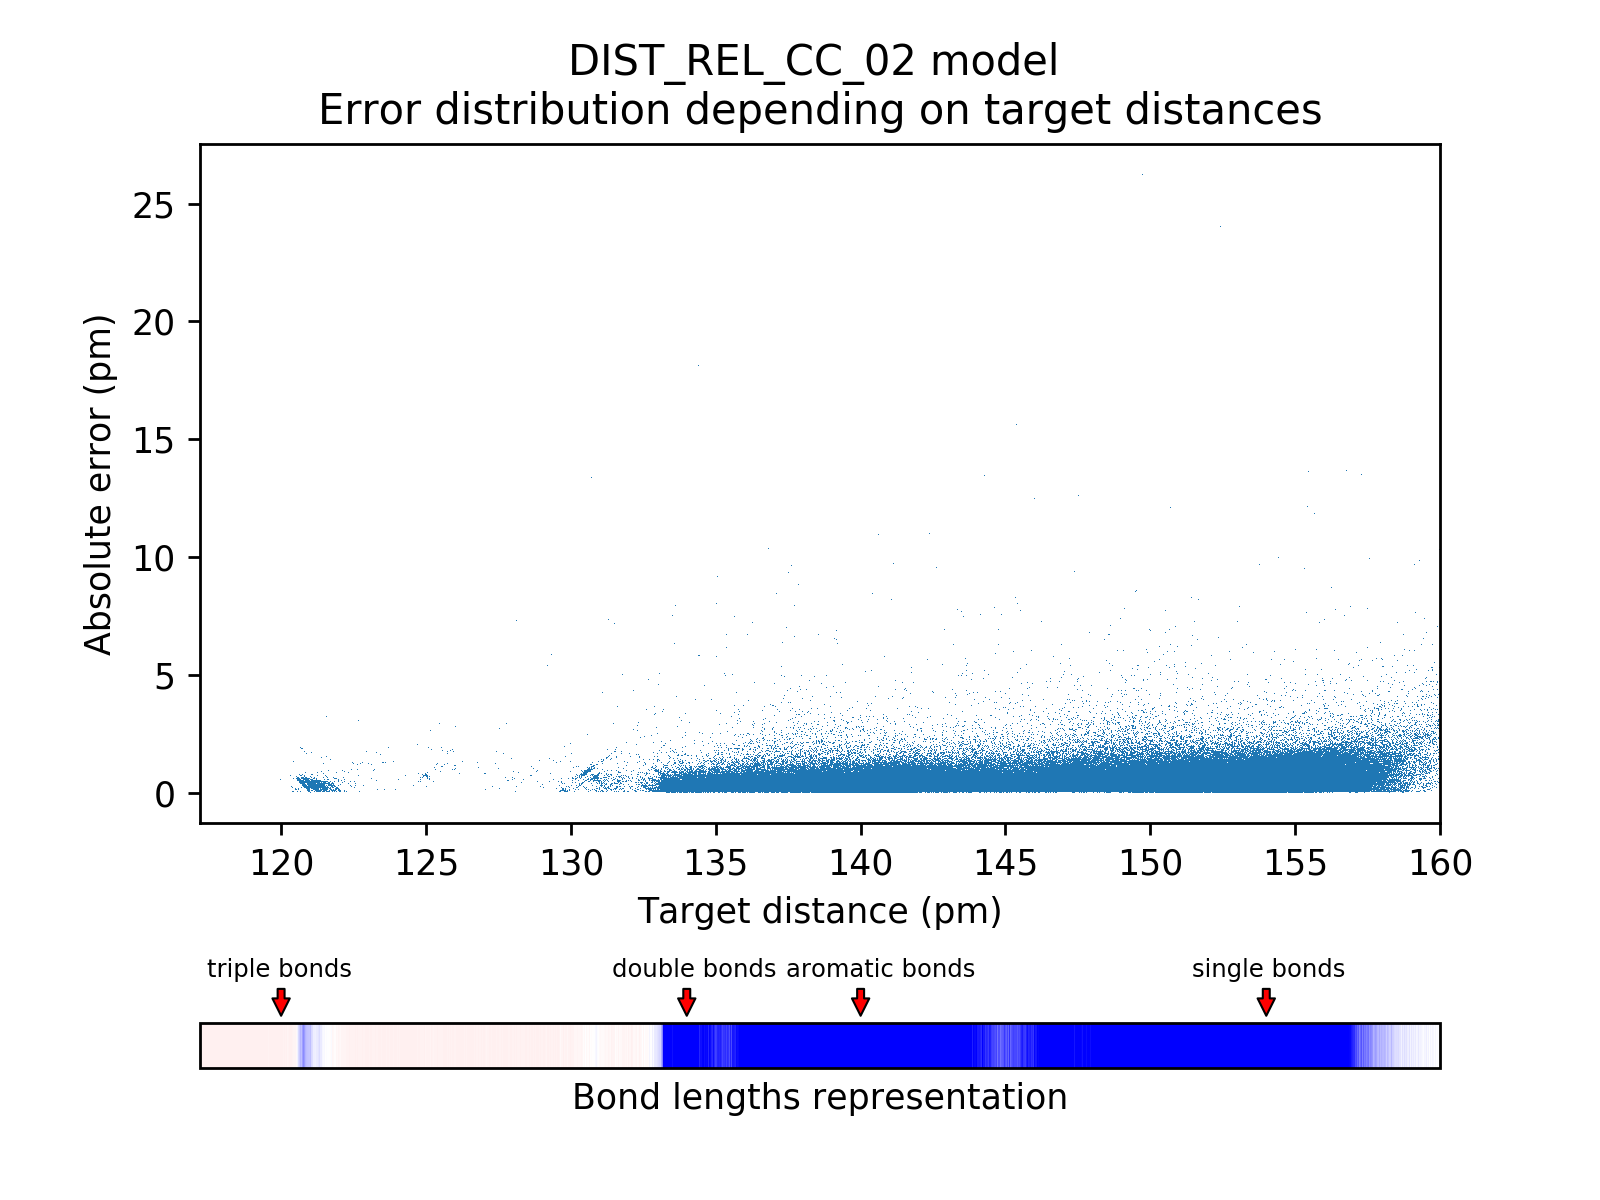
\includegraphics[scale=0.8]{../figures/DIST_REL_CC_02/DIST_REL_CC_02_distrib_rmse_dist.png}	
	
	\caption{Erreur en fonction des cibles pour le modèle \emph{DIST\_REL\_CC\_02}}
		\label{fdistrib_err_rel_dist_rel_cc_02}

	\end{figure}

\begin{figure}
	\centering
	
	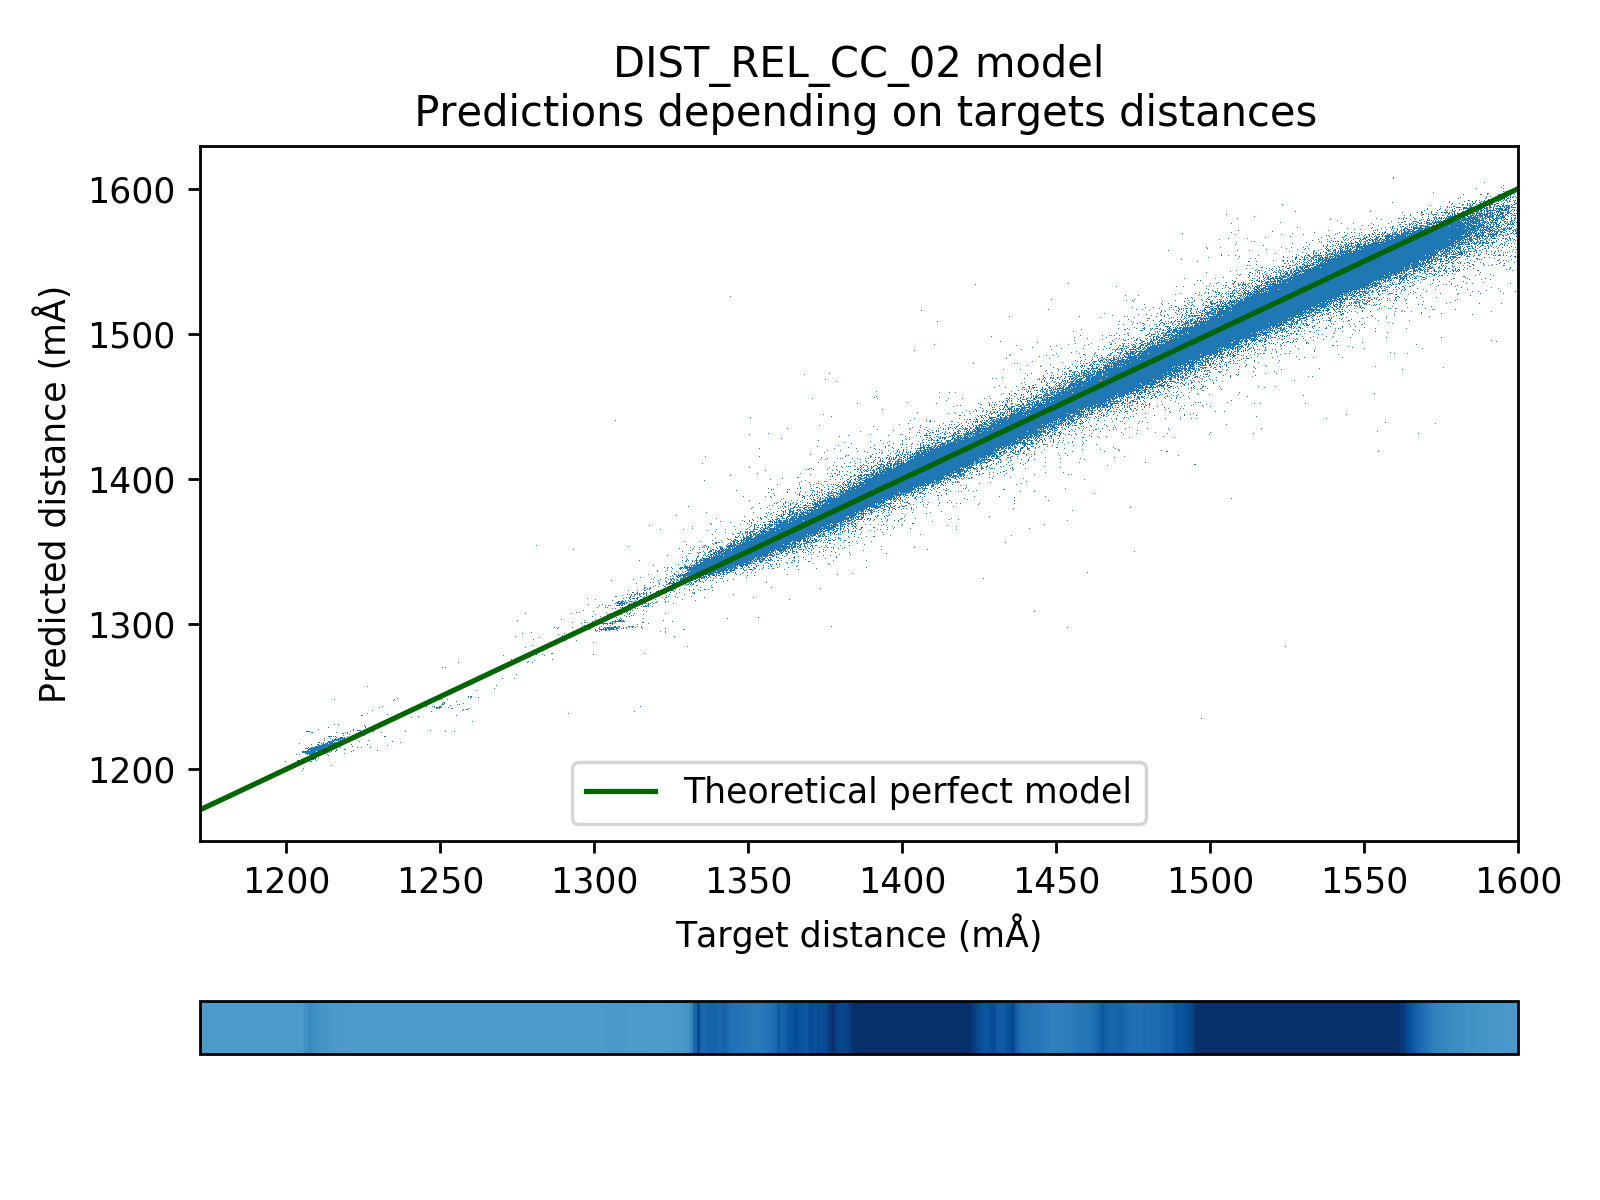
\includegraphics[scale=0.8]{../figures/DIST_REL_CC_02/DIST_REL_CC_02_preds_targets.png}	
	
	\caption{Prédictions en fonction des cibles pour le modèle \emph{DIST\_REL\_CC\_02}}
	\label{fpreds_targets_dist_rel_cc_02}
	
\end{figure}

\par La représentation graphique des erreurs et prédictions des deux autres modèles fait apparaître la légère amélioration des prédictions du modèle prédisant les longueurs de liaisons entre les atomes d'oxygène et d'hydrogène, et la baisse de performances du modèle prédisant les longueurs de liaisons entre les atomes de carbone et d'hydrogène. Elles sont disponibles en annexe \ref{annexes_plot_dist_rel_xy}.
	
\subsection{Application de fonctions aux distances}

\label{dist_rel_xy_fun}


\label{dist_rel_generalisation_fonctions}

\par L'application de fonctions aux distances en entrée des modèles (\ref{dist_rel_c_fun}) donne des résultats mitigés lorsqu'on tente de généraliser la méthode à plusieurs liaisons différentes sur des jeux d'entraînement plus grands. Les tableaux \ref{tstats_dist_rel_xy_03} et \ref{tstats_dist_rel_xy_04} présentent les valeurs des métriques évaluant les erreurs des modèles lorsqu'on applique la fonction inverse et carré de l'inverse aux distances en entrée. Les représentations graphiques des résultats sont disponibles en annexe \ref{annexes_plot_dist_rel_xy}. Notons que contrairement aux modèles de la première classe, le modèle \emph{DIST\_REL\_X\_03} (resp. \emph{DIST\_REL\_X\_04}) correspond à l'application de la fonction carré de l'inverse (resp. fonction inverse). Cela est dû au fait que seule la fonction carré de l'inverse devait être initialement appliquée, au vu de ses meilleurs résultats sur le modèle de la première classe. Ses résultats mitigés lors de la généralisation à d'autres liaisons nous ont cependant poussé à tester également la fonction inverse.\\
Notons enfin que les modèles décrits ici appliquent la restriction aux atomes au voisinage le plus proche (\ref{repr_locale_liaisons_cov_restrict}), avec une valeur $\epsilon$ de 200 pm.\\

\begin{table}
	\centering
	\begin{tabular}{|l|r|r|r|}
		\hline
		\textbf{Métrique}& \textbf{\emph{DIST\_REL\_CC\_03}} & \textbf{\emph{DIST\_REL\_CH\_03}} & \textbf{\emph{DIST\_REL\_OH\_03}}\\ \hline
		Moyenne & 0,4508 & 0,1634 & 0,2107\\ \hline
		Médiane &  0,3290 & 0,1206 &  0,1832\\ \hline
		Écart-type & 0,4582 & 0,1591 & 0,1742 \\ \hline
		Minimum & 0,0000 & 0,0000 & 0,0000\\ \hline
		Maximum & 16,6302 & 6.1820 & 7,0743 \\ \hline
		Erreur rel. & 0,3017\% & 0,1491\% & 0,2157\%\\ \hline
	\end{tabular}
	
	\caption{Analyse statistique des erreurs des modèles \emph{DIST\_REL\_XY\_03} (en pm)}
	\label{tstats_dist_rel_xy_03}
\end{table}

\begin{table}
	\centering
	\begin{tabular}{|l|r|r|r|}
		\hline
		\textbf{Métrique}& \textbf{\emph{DIST\_REL\_CC\_04}} & \textbf{\emph{DIST\_REL\_CH\_04}} & \textbf{\emph{DIST\_REL\_OH\_04}}\\ \hline
		Moyenne & 0,4727 & 0,1659 & 0,2478\\ \hline
		Médiane &  0,3773 & 0,1242 &  0,2080\\ \hline
		Écart-type & 0,4288 & 0,1564 & 0,2111 \\ \hline
		Minimum & 0,0000 & 0,0000 & 0.0000\\ \hline
		Maximum & 18,2097 & 7,2360 & 6,4610 \\ \hline
		Erreur rel. & 0,3182\% & 0,1514\% & 0.2535\%\\ \hline
	\end{tabular}
	
	\caption{Analyse statistique des erreurs des modèles \emph{DIST\_REL\_XY\_04} (en pm)}
	\label{tstats_dist_rel_xy_04}
\end{table}

\par On peut déjà remarquer que la relation d'ordre de la qualité des performances pour les deux fonctions est identique pour les deux classes de modèles, la fonction inverse du carré étant la plus efficace dans les deux cas. Lorsque l'on compare les prédictions des modèles prédisant les longueurs de liaisons carbone-carbone et hydrogène-oxygène, on s'aperçoit que l'application des deux fonctions détériore la qualité générale des résultats, même si elle permet de diminuer les erreurs maximales. On peut raisonnablement en déduire que ces fonctions ne sont pas optimales pour décrire l'intensité de l'influence des atomes au voisinage d'une liaison en fonction de leur distance aux atomes de la liaison, et qu'il est plus simple pour les réseaux de neurones d'approximer la fonction optimale à partir des distances brutes que des distances transformées.
\par Les résultats des prédictions pour les distances entre les atomes de carbone et d'hydrogène sont toutefois très surprenants. En effet, l'application du carré de l'inverse sur les distances les améliore d'un facteur deux. \\
La disparité de ces résultats les rend toutefois difficiles à interpréter. Il faudrait entraîner tous les modèles plusieurs fois sur des données différentes afin d'évaluer la dispersion de leurs résultats. Nous ne pouvons en effet pas affirmer que les différences entre les résultats que nous observons ici ne sont pas dues au hasard des différentes exécutions, même si le fait que la relation d'ordre entre les performances des deux fonctions soit constante sur les différents modèles laisse  penser que l'application des fonctions améliore la prédiction des liaisons CC et OH, et détériore la prédiction des liaisons CH.\\
\par Il semble que nous soyons face à un problème complexe, et qu'il n'existe pas un type de modèle et une représentation des données uniques permettant de prédire de façon optimale tous les types de liaisons au sein des molécules.


	\section{Ouverture à d'autres modèles d'apprentissage automatique}
		\par Dans le but de comparer les modèles basés sur des réseaux de neurones artificiels que l'on entraîne à d'autres modèles prédictifs d'apprentissage automatique, nous entraînons deux modèles de régression linéaire à effectuer les mêmes tâches. Ces modèles sont une régression d'arête (\emph{ridge regression}) avec l'astuce du noyau (\emph{kernel trick}), et une machine à vecteur de support (SVM). Nous utilisons pour cela les implémentations fournies par la bibliothèque Scikit-Learn\cite{sklearn}. L'implémentation de ces deux modèles est identique, à la différence que le modèle \emph{Kernel Ridge Regression} (KRR) utilise le carré des erreurs comme fonction de coût, alors que le modèle SVM utilise une fonction $\epsilon$-insensible, c'est à dire que les erreurs coûtent leur valeur brute, ou valent zéro si elles sont inférieures à un seuil $\epsilon$ donné.
\\

\subsection{Données d'entrée et complexité algorithmique}

\par Afin d'avoir une idée des performances relatives de tous ces modèles, nous les entraînons à prédire les distances relatives entre des atomes de carbone formant une liaison. Ces modèles sont équivalents au modèle \emph{DIST\_REL\_C\_05} (REF DIST REL C 05), car on applique une restriction aux atomes les plus proches de la liaison, et on limite la largeur des entrées à 15 atomes. Ce choix de données d'entrée est lié à la nécessité de fournir des entrées de petite taille (comparativement aux données que l'on donne aux réseaux de neurones) à ces modèles, qui ont une complexité d'entraînement augmentant très vite avec le nombre et la taille des exemples. Avec $n$ le nombre d'exemples et $m$ leur largeur, la complexité de l'entraînement d'un modèle SVM varie entre $O(n^2\times m)$ et $O(n^3\times m)$. La complexité de l'entraînement des modèles KRR n'est pas disponible dans la documentation de Scikit-Learn, mais elle plus grande encore que celle des SVM.
\par Pour la même raison, le nombre d'exemples dans les jeux d'entraînement de ces modèles est beaucoup plus faible que celui des jeux utilisés pour entraîner les réseaux de neurones artificiels. Les modèles que l'on décrit dans cette partie s'entraînent sur des jeux contenant 60000 exemples, ce qui représente tout de même environ cinq jours de temps CPU pour l'entraînement d'un modèle KRR.
\par Enfin, la fonction inverse est appliquée aux distances dans les données d'entrée de ces modèles. En effet, si les réseaux de neurones artificiels sont capables d'approximer ces fonctions, ce n'est pas le cas des modèles que l'on entraîne ici. L'application de la fonction inverse permet de donner des coefficients aux modèles exprimant l'influence des atomes au voisinage des liaisons en fonction de leur distance.

\subsection{Entraînement de modèles KRR}

\subsubsection{Recherche par quadrillage des paramètres}
Afin d'entraîner un modèle fournissant de bons résultats, nous commençons par effectuer une recherche par quadrillage avec trois validations croisées des paramètres pour le modèle KRR. Cette recherche est effectuée sur la grille de paramètres suivante. Selon la documentation, une valeur faible du paramètre alpha va diminuer la variance des erreurs. Le degré correspond au degré du polynôme, et le paramètre coef0 correspond au coefficient constant du polynôme. Les résultats de la recherche par quadrillage sont donnés en annexe (REF ANNEXES QUADRI KER RIDGE).

\begin{figure}[!h]
	\centering
	
	\begin{tabular}{|l|l|}
		\hline
		\textbf{Paramètres} & \textbf{Valeurs} \\ \hline 
		Noyau (\emph{kernel}) & linéaire\\ \hline
		Alpha & 0.1, 0.01, 0.001 \\ \hline
	\end{tabular}
	
	\vspace{0.5cm}	

	\begin{tabular}{|l|l|}
		\hline
		\textbf{Paramètres} & \textbf{Valeurs} \\ \hline 
		Noyau (\emph{kernel}) & polynomial\\ \hline
		Degré & 2, 6 \\ \hline
		Alpha & 0.1, 0.01, 0.001 \\ \hline
		Coef0 & 1, 0.5, 2 \\ \hline
	\end{tabular}		
	
	\caption{Grille de recherche par quadrillage des paramètres pour les modèles KRR}
\end{figure}

\subsubsection{Entraînement d'un modèle et analyse des prédictions}
\par À l'issue de la recherche par quadrillage, on utilise les meilleurs paramètres pour entraîner un modèle KRR (\emph{DIST\_REL\_C\_KER\_RIDGE\_01}) sur les 60000 exemples de notre jeu d'entraînement. Les paramètres sont donnés dans le tableau suivant.

\begin{figure}[!h]
	\centering
	\begin{tabular}{|l|l|}
		\hline
		\textbf{Paramètre} & \textbf{Valeur} \\ \hline
		Noyau & polynomial \\ \hline
		Degré & 2 \\ \hline
		Alpha & 0.01 \\ \hline
		Coef0 & 1 \\ \hline
	\end{tabular}		
	\caption{Paramètres d'entraînement du modèle \emph{DIST\_REL\_C\_KER\_RIDGE\_01}}
\end{figure}

\par Les valeurs des métriques évaluant les erreurs sont données dans le tableau suivant. On y voit que le modèle est très performant pour un premier ensemble de paramètres issu d'une petite recherche par quadrillage. L'erreur médiane est en effet de l'ordre du demi picomètre et l'erreur moyenne de l'ordre du picomètre.

\begin{figure}[!h]
	\centering
	\begin{tabular}{|l|r|}
		\hline
		\textbf{Métrique} & \textbf{Valeur} \\ \hline
		Moyenne & 1,0378 \\ \hline
		Médiane & 0,5891 \\ \hline
		Écart-type & 1,2668 \\ \hline
		Minimum & 0,0000 \\ \hline
		Maximum & 21,6264\\ \hline
		Erreur relative moyenne & 0.7057\% \\ \hline
	\end{tabular}
	
	\caption{Analyse statistique des erreurs du modèle \emph{DIST\_REL\_C\_KER\_RIDGE\_01} (en pm)}
\end{figure}

\par La représentation graphique de la distribution des erreurs et des prédictions disponible dans les figures ci-dessous montre que les erreurs au delà de 10 pm sont très minoritaires, mais montre également que le modèle prédit difficilement les distances peu représentées, à la limite entre les différents types de liaisons.
\par Pour résumer, les modèles prédictifs de type KRR semblent permettent d'obtenir des prédictions proches de la précision requise et pourraient donc être utilisés pour prédire la géométrie convergée complète d'une molécule (REF MODULES), notamment dans le cas des liaisons qui sont peu représentées dans les données, et pour lesquelles les modèles prédictifs basés sur des réseaux de neurones artificiels seront probablement moins efficaces.

\begin{figure}[!h]
	\centering
	
	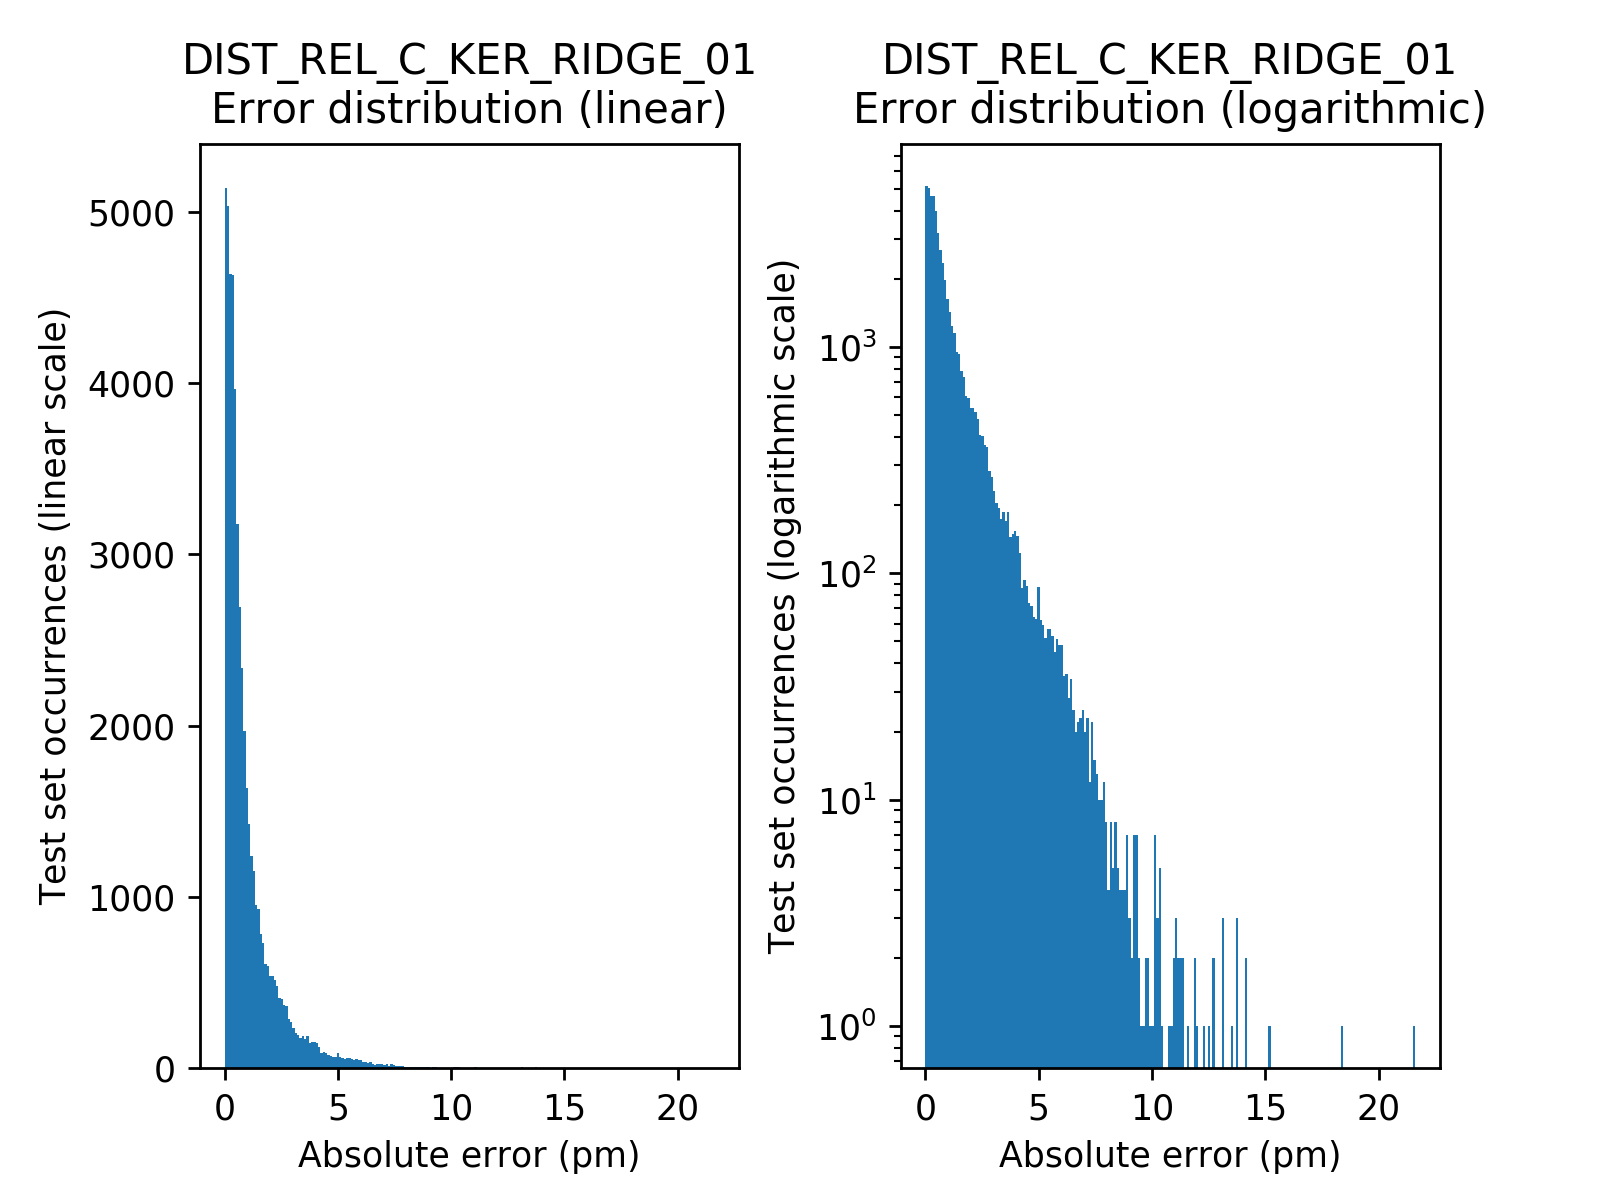
\includegraphics[scale=0.8]{../figures/DIST_REL_C_KER_RIDGE_01/DIST_REL_C_KER_RIDGE_01_distrib_rmse_val.png}	
	
	\caption{Distribution des erreurs du modèle \emph{DIST\_REL\_C\_KER\_RIDGE\_01}}
\end{figure}
\begin{figure}[!h]
	\centering
	
	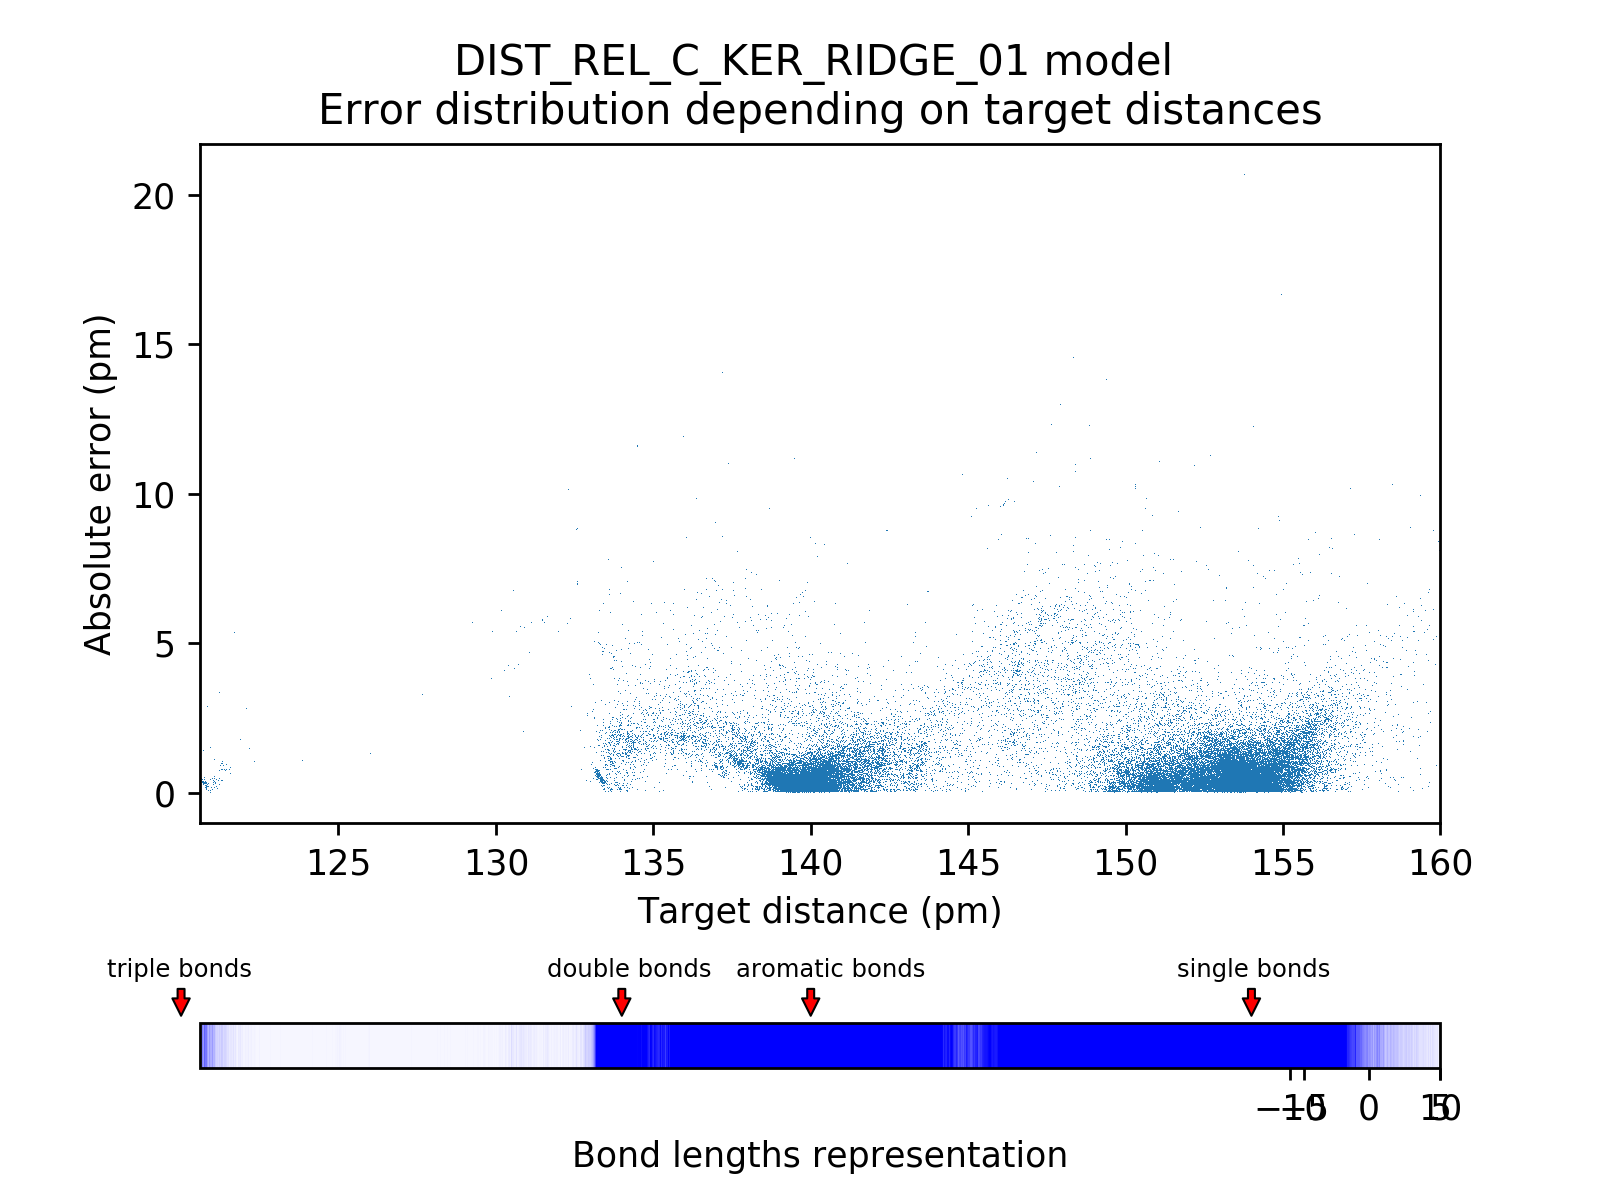
\includegraphics[scale=0.8]{../figures/DIST_REL_C_KER_RIDGE_01/DIST_REL_C_KER_RIDGE_01_distrib_rmse_dist.png}	
	
	\caption{Erreur en fonction des cibles pour le modèle \emph{DIST\_REL\_C\_KER\_RIDGE\_01}}
	\end{figure}

\begin{figure}[!h]
	\centering
	
	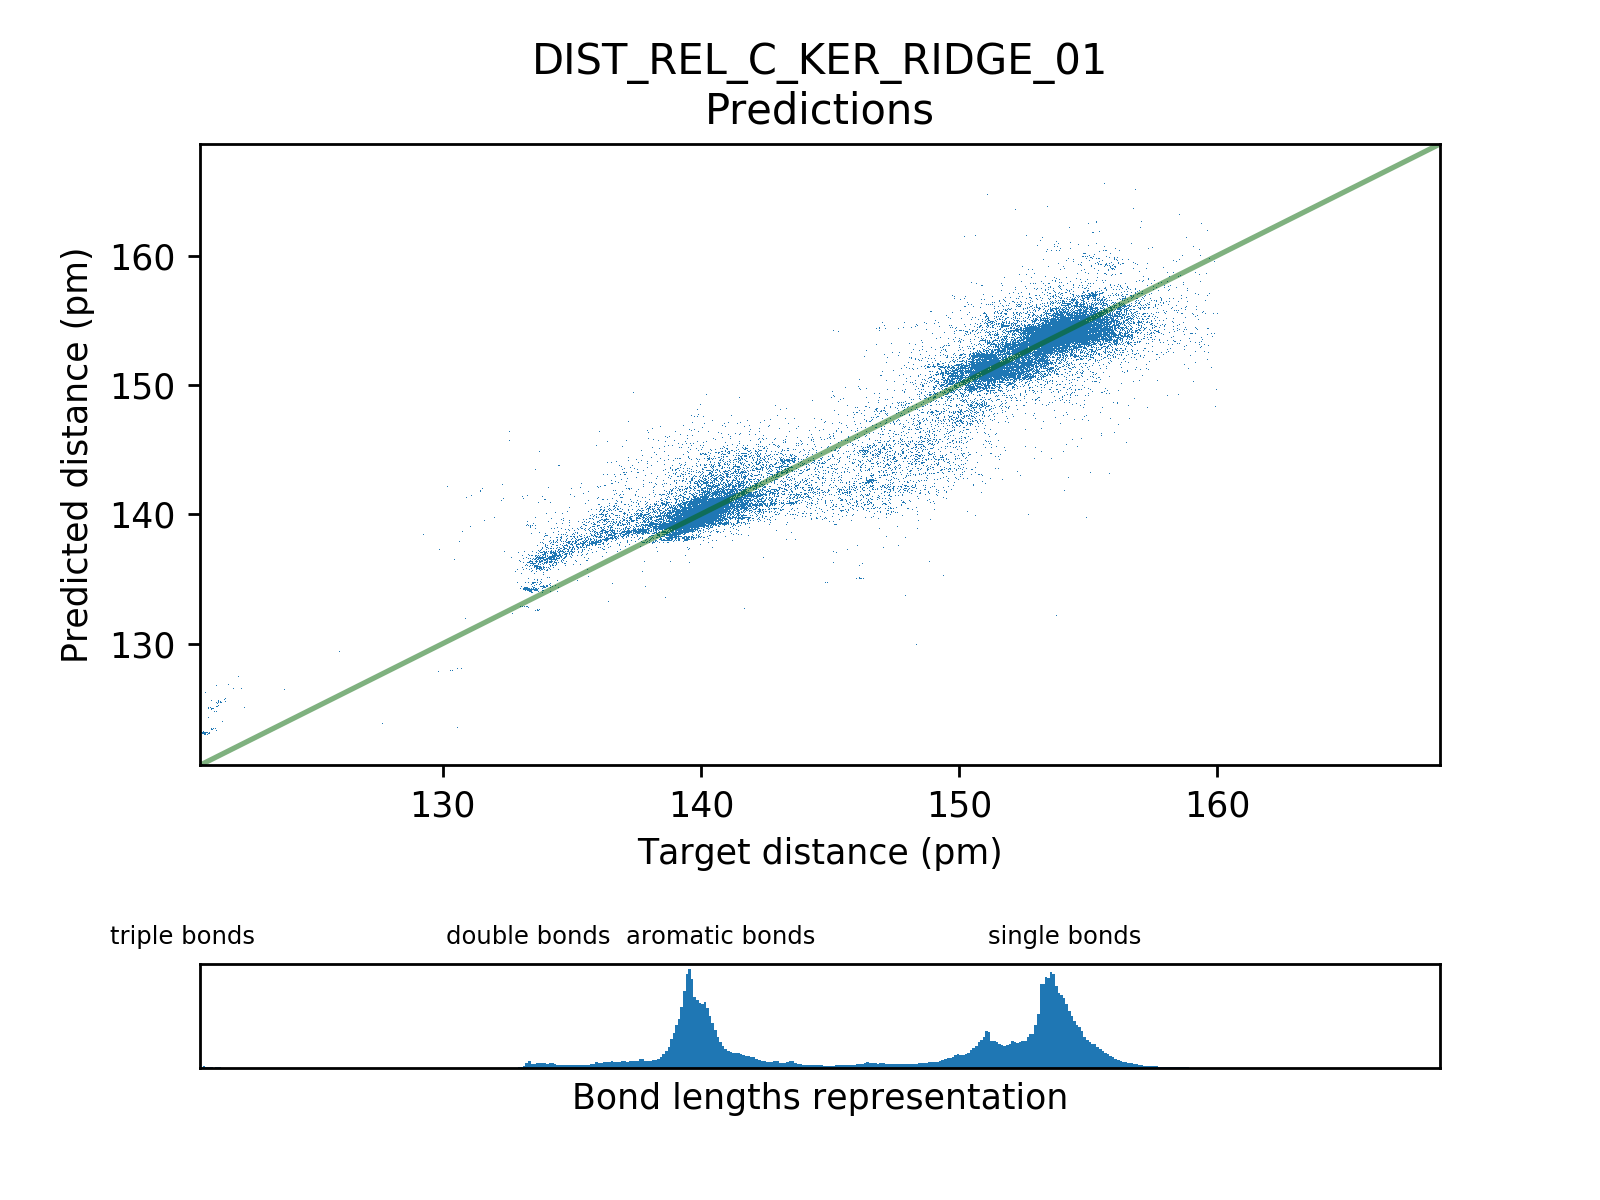
\includegraphics[scale=0.8]{../figures/DIST_REL_C_KER_RIDGE_01/DIST_REL_C_KER_RIDGE_01_preds_targets.png}	
	
	\caption{Prédictions en fonction des cibles pour le modèle \emph{DIST\_REL\_C\_KER\_RIDGE\_01}}
	
\end{figure}

\subsection{Entraînement de modèles SVM}

\subsubsection{Recherche par quadrillage des paramètres (non aboutie)}
Dans l'idée d'appliquer la même méthodologie que pour le modèle de type KRR, nous définissons une grille de recherche par quadrillage des paramètres des modèles SVM. Cette grille est en revanche plus large, puisqu'elle définit l'entraînement de 256 modèles différents avec trois validations croisées, soit l'entraînement de 768 modèles.
La grille de paramètres utilisée est disponible dans la figure ci-dessous. Malheureusement, la recherche n'a pas abouti car certains ensembles de paramètres menaient à l'entraînement de modèles en un temps non raisonnable. Parmi les modèles de la grille, 747 ont été entraînés en environ deux minutes, tandis que l'entraînement des 21 restants n'était pas terminé au bout d'une dizaine d'heures, ce qui a mené à l'interruption de la recherche.

\begin{figure}[!h]
	\centering
	
	\begin{tabular}{|l|l|}
		\hline
		\textbf{Paramètres} & \textbf{Valeurs} \\ \hline 
		Noyau (\emph{kernel}) & linéaire\\ \hline
		$\epsilon$ (fonction de coût) & 0.1, 0.001 \\ \hline
		Coef0 & 0, 0.1, 0.5, 1 \\ \hline
		Heuristique de rétrécissement (\emph{Shrinking}) & True, False \\ \hline
		Tolérance de l'arrêt de l'optimisation & 0.001, 0.01 \\ \hline
		Pénalité sur le terme d'erreur (C) & 1, 0.01\\ \hline
	\end{tabular}
	
	\vspace{0.5cm}	

	\begin{tabular}{|l|l|}
		\hline
		\textbf{Paramètres} & \textbf{Valeurs} \\ \hline 
		Noyau (\emph{kernel}) & polynomial\\ \hline
		$\epsilon$ (fonction de coût) & 0.1, 0.001 \\ \hline
		Gamma (coefficient utilisé par le noyau) & auto, 0.001, 0.01 \\ \hline
		Coef0 & 0, 0.1, 0.5, 1 \\ \hline
		Heuristique de rétrécissement (\emph{Shrinking}) & True, False \\ \hline
		Tolérance de l'arrêt de l'optimisation & 0.001, 0.01 \\ \hline
		Pénalité sur le terme d'erreur (C) & 1, 0.01\\ \hline
	\end{tabular}		
	
	\caption{Grille de recherche par quadrillage des paramètres pour les modèles SVM}
\end{figure}

\subsubsection{Entraînement d'un modèle et analyse des prédictions}
\par La recherche par quadrillage des paramètres n'ayant pas abouti, nous utilisons les paramètres issus de la recherche par quadrillage pour le modèle de type KRR, dans l'idée qu'ils devraient permettre également d'obtenir de bons résultats, et nous laissons les autres paramètres à leur valeur par défaut. Les statistiques des erreur du modèle alors entraîné sont donné dans le tableau suivant. Notons que le fait que le numéro chronologique du modèle soit « 03 » est la conséquence de l'entraînement de deux modèles préalables dont le but était d'estimer le temps d'entraînement en fonction de la taille des données d'entrée.\\

\begin{figure}[!h]
	\centering
	\begin{tabular}{|l|r|}
		\hline
		\textbf{Métrique} & \textbf{Valeur} \\ \hline
		Moyenne & 1,2854 \\ \hline
		Médiane & 0,5005 \\ \hline
		Écart-type & 2,2301 \\ \hline
		Minimum & 0,0000 \\ \hline
		Maximum & 24,2225\\ \hline
		Erreur relative moyenne & 0.8907\% \\ \hline
	\end{tabular}
	
	\caption{Analyse statistique des erreurs du modèle \emph{DIST\_REL\_C\_SVM\_03} (en pm)}
\end{figure}

\par Les statistiques comme les figures suivantes représentant graphiquement les erreurs et les prédictions du modèle disponibles montrent que ses résultats sont nettement inférieurs aux modèles précédents. Le modèle se contente en effet de prédire des valeurs de l'ordre des deux types de liaisons les plus représentées, et ne prédit pas correctement les longueurs de liaisons de tailles intermédiaires.\\


\begin{figure}[!h]
	\centering
	
	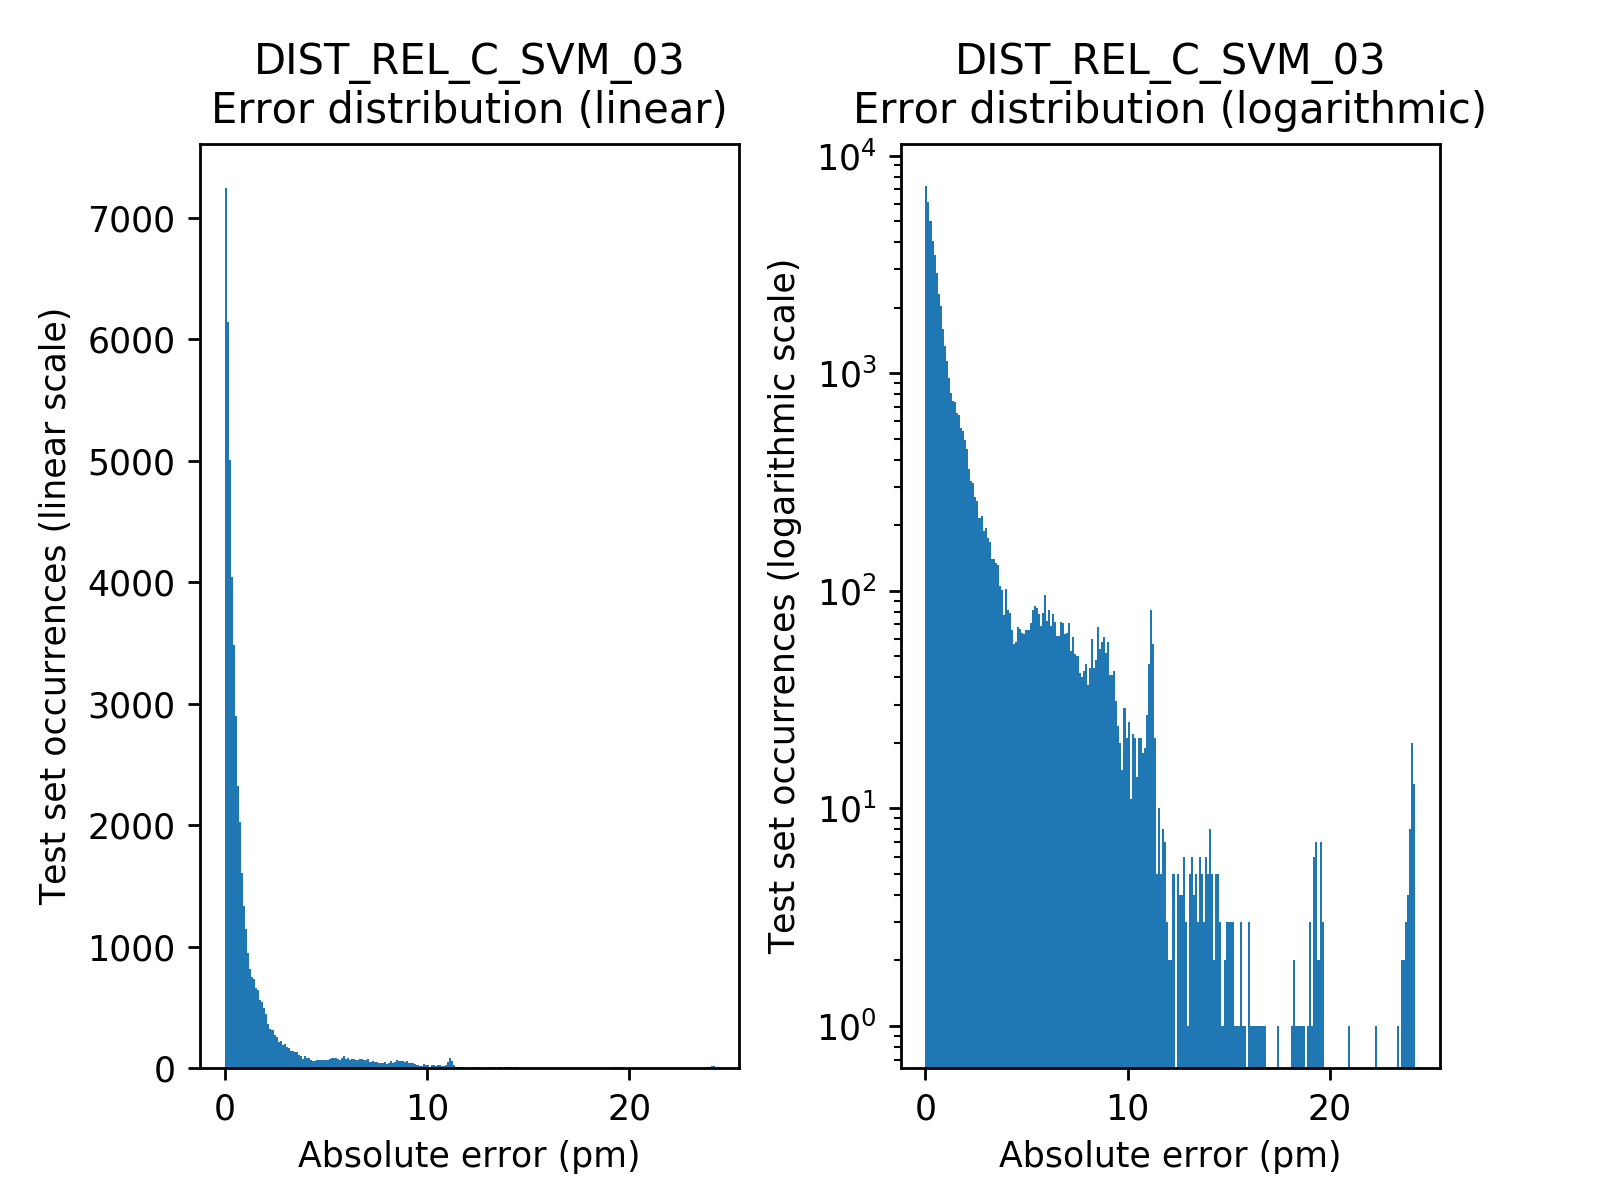
\includegraphics[scale=0.8]{../figures/DIST_REL_C_SVM_03/DIST_REL_C_SVM_03_distrib_rmse_val.png}	
	
	\caption{Distribution des erreurs du modèle \emph{DIST\_REL\_C\_SVM\_03}}
\end{figure}
\begin{figure}[!h]
	\centering
	
	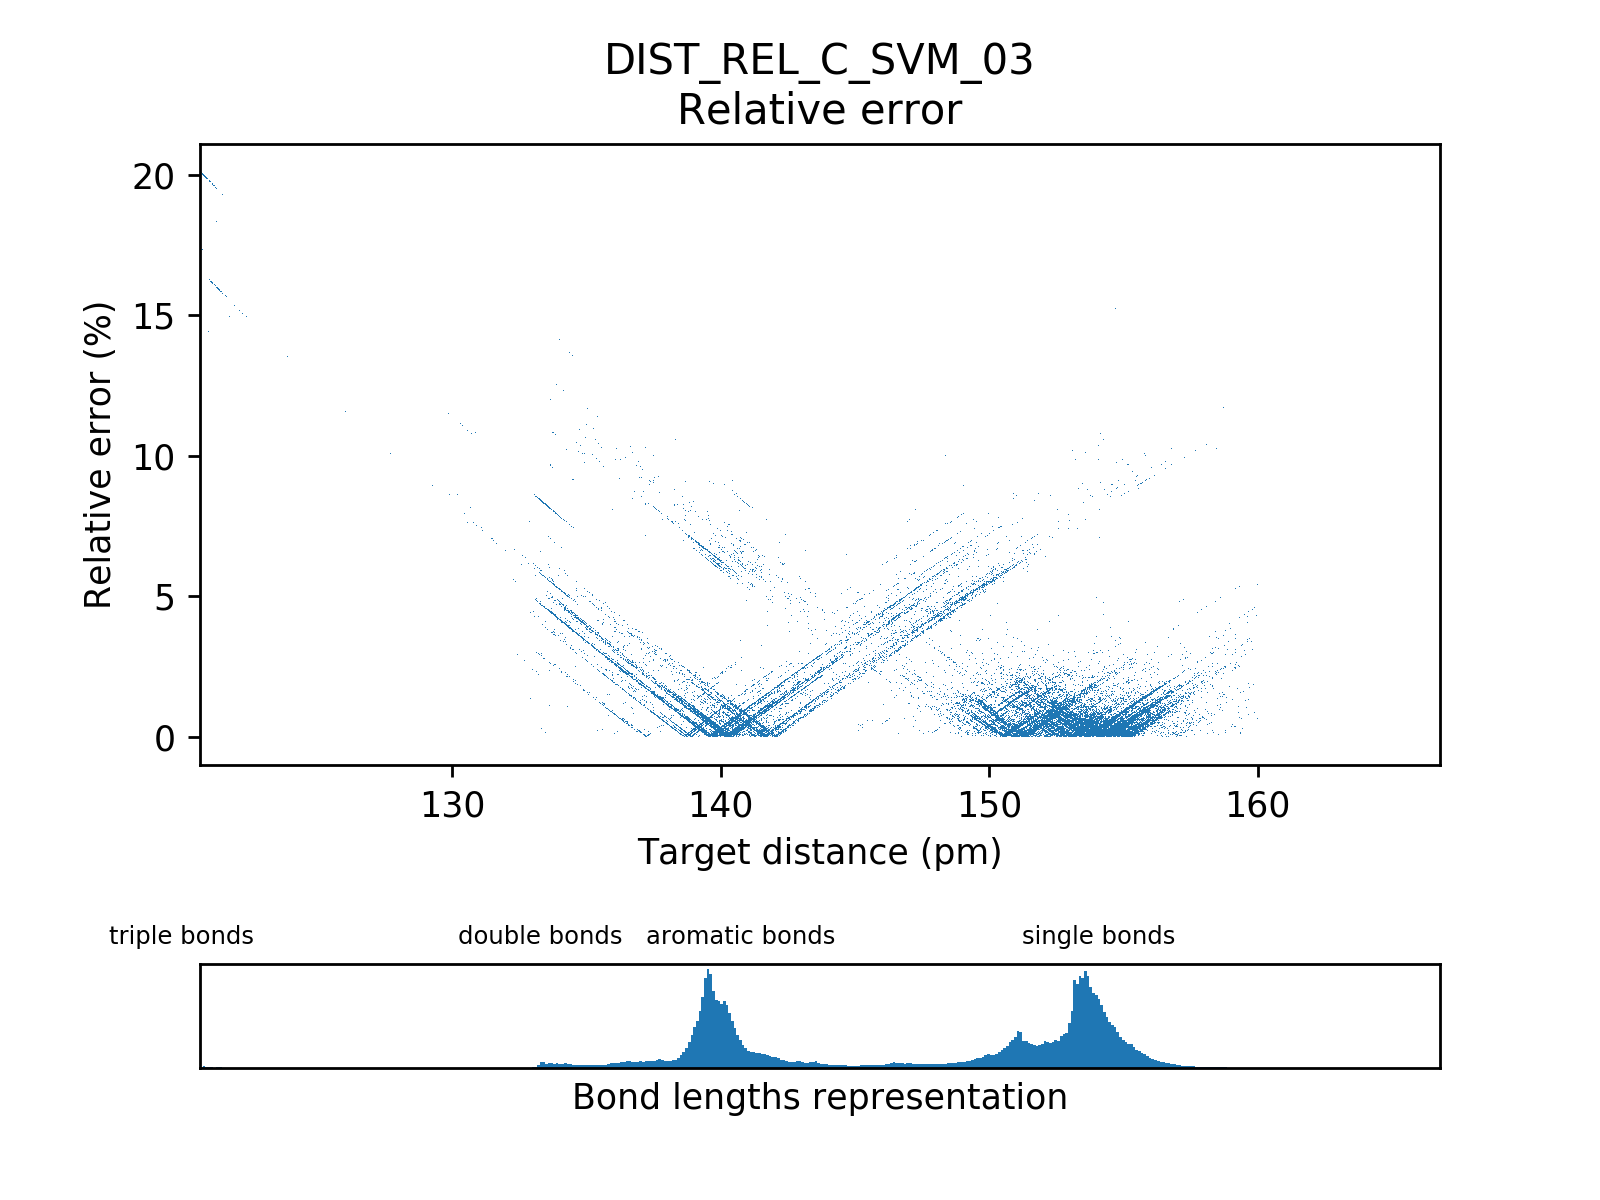
\includegraphics[scale=0.8]{../figures/DIST_REL_C_SVM_03/DIST_REL_C_SVM_03_distrib_rmse_dist.png}	
	
	\caption{Erreur en fonction des cibles pour le modèle \emph{DIST\_REL\_C\_SVM\_03}}
	\end{figure}

\begin{figure}[!h]
	\centering
	
	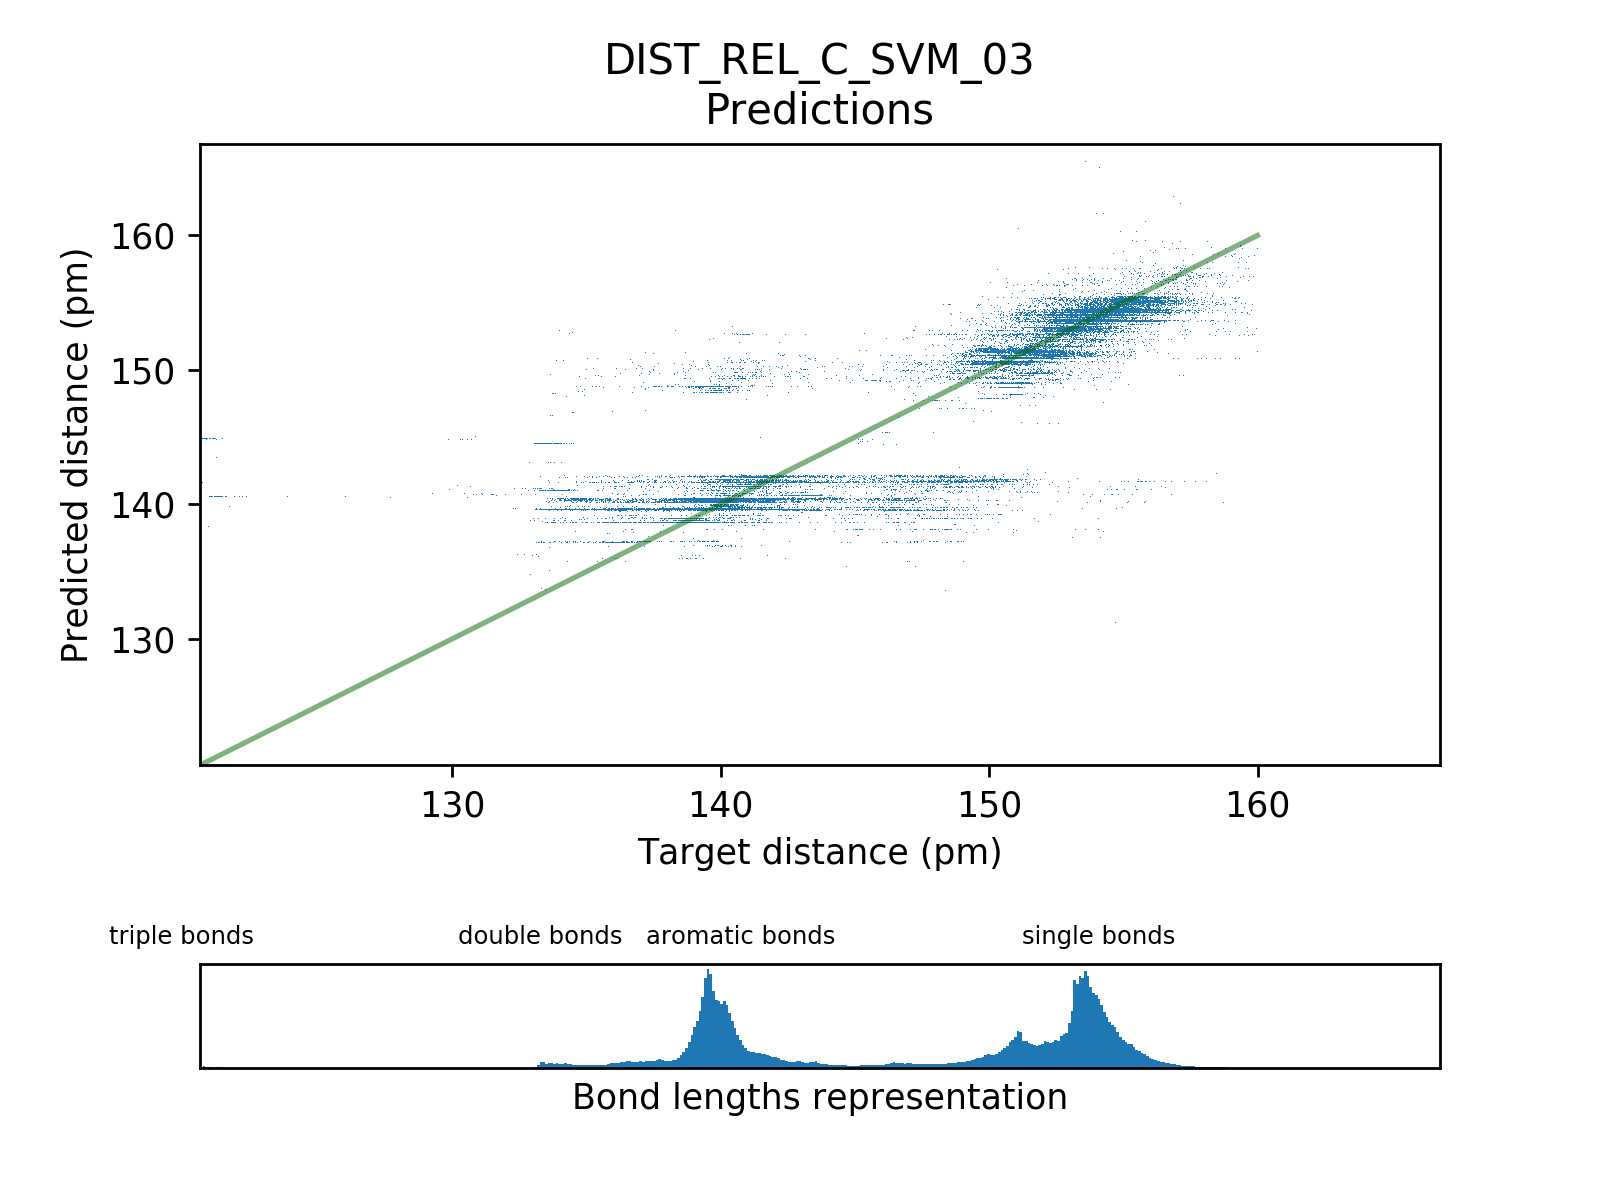
\includegraphics[scale=0.8]{../figures/DIST_REL_C_SVM_03/DIST_REL_C_SVM_03_preds_targets.png}	
	
	\caption{Prédictions en fonction des cibles pour le modèle \emph{DIST\_REL\_C\_SVM\_03}}
	
\end{figure}




\chapter{Prédiction de géométries moléculaires convergées}

	\section{Introduction}
		\subsection{Motivation}
			\par L'objectif des modèles prédictifs que l'on décrit dans ce chapitre est de prédire la géométrie convergée (REF GEOM CONVERG) d'une molécule complète, à partir d'une géométrie non convergée. Ils sont issus d'une tentative de reproduction de résultats antérieurs, afin de confirmer la méthode élaborée lors des stages précédents sur le projet QuChemPedIA.\\
Chronologiquement, ces modèles ont constitué la première partie de mon travail, avant de passer aux modèles tentant de prédire les longueurs de liaisons (REF DIST\_REL), à cause de l'impossibilité de produire des prédictions de qualité suffisante (REF RESULTATS).\\

\par L'objectif à terme de ces modèles est de pouvoir constituer une alternative au DFT (REF DFT) pour calculer rapidement la géométrie convergée d'une molécule. Cela nécessite de produire des prédictions d'une très grande précision. Cependant, le but ici est avant tout de valider une méthode et notre capacité à produire des prédictions d'ordre géométrique. Nous ne cherchons donc pas à créer un modèle effectuant de très bonnes prédictions, mais plutôt à définir une représentation des données et un ensemble de paramètres permettant d'obtenir de bons résultats.

\paragraph{Introduction de bruit} Afin de prédire des géométries moléculaires convergées à partir de géométries moléculaires non convergées, la situation idéale serait que les modèles apprennent à partir d'un ensemble de géométries non convergées issues de mesures ou d'optimisation par mécanique moléculaire (REF MÉCA MOL), et l'ensemble de géométries convergées par le DFT (REF DFT) associé. Cela constituerait en effet un ensemble de données homogène qui aurait l'avantage d'être comparable aux données que l'on utiliserait dans un cas d'utilisation réel.\\
Malheureusement, nous ne possédons pas de telles données. Nous possédons les géométries convergées issues de la base PubChemQC (REF PUBCHEMQC) mais pas les géométries à partir desquelles elles ont été calculées. S'il est théoriquement possible de calculer la géométrie optimisée en mécanique moléculaire de toutes les molécules de la base PubChemQC en utilisant le programme Open Babel\footnote{\url{http://openbabel.org/wiki/Main_Page}}, la perte de l'ordre des atomes lors de l'optimisation rend la procédure impossible en pratique.\\
L'alternative retenue lors des stages précédents est d'introduire du bruit (REF PREP DONNEES BRUIT) dans les coordonnées des géométries optimisées, et d'entraîner les modèles à prédire ce bruit. La différence entre la géométrie bruitée et le bruit prédit permet alors d'obtenir la géométrie optimisée par le modèle. L'introduction de bruit ne garantit donc pas que les modèles se généraliseront aux données réelles, mais semble tout de même raisonnable pour tenter de valider la méthode, puisque nous entraînons des modèles dont l'objectif est de déplacer les atomes d'une molécule de sorte à obtenir une géométrie convergée.

\paragraph{Modèles} Cinq modèles différents ont été entraînés. Ils diffèrent par les représentations utilisées en entrée et en sortie, les caractéristiques des molécules dont on tente de prédire la géométrie convergée, et les paramètres propres aux réseaux de neurones comme les fonctions de coût ou la topologie. Nous allons répertorier les différentes caractéristiques utilisées mais pas modèle par modèle, puisque aucun ensemble de caractéristiques n'a produit de résultats significativement meilleurs que les autres (REF RESULTATS). Cependant, une table des caractéristiques utilisées modèle par modèle est disponible en annexe (REF CARAC ANNEXES).



		\subsection{Méthodologie}
			\paragraph{Introduction de bruit} Afin de prédire des géométries moléculaires convergées à partir de géométries moléculaires non convergées, la situation idéale serait que les modèles apprennent à partir d'un ensemble de géométries non convergées issues de mesures ou de résultats théoriques, et l'ensemble associé de géométries convergées issu de l'optimisation géométrique quantique (REF DFT). Cela constituerait en effet un ensemble de données homogène qui aurait l'avantage d'être comparable aux données que l'on utiliserait dans un cas d'utilisation réel.\\
La solution retenue lors des stages précédents est d'introduire du bruit (REF PREP DONNEES BRUIT) dans les coordonnées des géométries optimisées, et d'entraîner les modèles à prédire ce bruit. La différence entre la géométrie bruitée et le bruit prédit permet alors d'obtenir la géométrie optimisée par le modèle. L'introduction de bruit ne garantit donc pas que les modèles se généraliseront aux données réelles, mais semble tout de même raisonnable pour tenter de valider la méthode, puisque nous entraînons des modèles dont l'objectif est de déplacer les atomes d'une molécule de sorte à obtenir une géométrie convergée.

\paragraph{Modèles} Cinq modèles différents ont été entraînés. Ils diffèrent par les représentations utilisées en entrée et en sortie, les caractéristiques des molécules dont on tente de prédire la géométrie convergée, et les paramètres propres aux réseaux de neurones comme les fonctions de coût ou la topologie. Dans la section suivante, nous allons répertorier les différentes caractéristiques utilisées de façon non chronologique, puisque aucun ensemble de caractéristiques n'a produit de résultats significativement meilleurs que les autres (REF RESULTATS). Cependant, une table des caractéristiques utilisées modèle par modèle est disponible en annexe (REF CARAC ANNEXES).
		\subsection{Nomenclature}
			Afin de simplifier leur dénomination, on nomme les différents modèles prédictifs. Tous les modèles décrits dans ce chapitre ont un nom de préfixe « DELTA\_DIST\_+H », issu de leur vocation à prédire des différences ($\Delta$) de distances pour obtenir des géométries convergées. Le suffixe « +H » indique que les données d'entrée contiennent les informations concernant les atomes d'hydrogène. Initialement, des modèles ne contenant pas les atomes d'hydrogène en entrée devaient être créés par la suite, mais ce projet a été abandonné faute de pouvoir obtenir des résultats satisfaisants avec le modèle actuel (REF RESULTATS).\\
Le nom des modèles possède enfin comme suffixe leur numéro chronologique.
			
	\section{Données et paramètres des modèles}
		\subsection{Données}
			\subsubsection{Représentations géométriques}
\par Les modèles que l'on entraîne devant prédire la géométrie des molécules, nous devons leur fournir des données utilisant des représentations synthétisant de la façon la plus simple possible la position des atomes. Nous ne donnons pas les coordonnées brutes aux modèles car ils devraient leur appliquer trop de traitements (REF MAT POS).\\
Les modèles élaborés lors des stages antérieurs utilisaient la représentation géométrique par matrice réduite des distances inter-atomiques (REF MAT. RED. DIST). Elle est basée sur les distances relatives des atomes et possède donc l'avantage d'être indépendante de tout repère absolu. Cependant, il n'est pas possible de reconstruire systématiquement une matrice des positions atomiques à l'issue des prédictions des modèles utilisant cette représentation en sortie. C'est pourquoi nous avons abandonné cette représentation cette année au profit de la matrice des distances à des points fixes (REF MAT PTS FIXES), qui dépend d'un repère absolu mais dont on peut toujours déduire une matrice des positions atomiques.\\

\par Nous avons toutefois entraîné deux modèles de noms DELTA\_DIST\_+H\_03 (resp. DELTA\_DIST\_+H\_04) utilisant comme entrée les deux représentations et comme sortie la représentation par matrice des distances à des points fixes (resp. matrice réduite des distances inter-atomiques). L'entraînement du premier de ces modèles avait pour but de tester si la représentation en repère relatif permettait d'obtenir de meilleurs résultats, et l'entraînement du second avait pour but de vérifier si les mauvaises performances des modèles s'expliquaient par l'utilisation d'une représentation dans un repère absolu. Notons que ce dernier modèle avait uniquement une vocation de test, puisque l'on n'aurait pas été capables de construire la matrice des positons atomiques à l'issue des prédictions, et que l'on n'aurait donc pas pu l'utiliser dans un cas d'utilisation réel.\\

\par Nous avons également utilisé une variante de la représentation par matrice des distances à des points fixes comme entrée de l'un des modèles (DELTA\_DIST\_+H\_02). Dans cette variante, les points fixes de référence sont considérés comme des atomes fictifs et leurs distances relatives sont donc données. Elles avaient initialement été ignorées car elles sont constantes et les réseaux de neurones sont donc théoriquement capables de les \emph{déduire}. Ce modèle permettait de s'assurer que les mauvais résultats ne sont pas dus à cette information manquante.

\subsubsection{Propriétés atomiques}
\par En plus de la géométrie des molécules, nous donnons aux modèles des informations concernant chaque atome et ayant une influence sur la géométrie convergée. Tous les modèles que l'on a entraînés possèdent en entrée la masse atomique de chaque atome, et un des modèles (DELTA\_DIST\_+H\_05) possède également les numéros atomiques. De même que pour les distances entre les points du repère, il s'agit d'une information que les réseaux de neurones sont capables de déduire, nous la donnons pour nous assurer que les mauvais résultats ne sont pas dus à son absence.

\subsubsection{Bruit}
\par L'introduction de bruit dans la géométrie moléculaire convergée et le déplacement des atomes selon les prédictions des modèles pour obtenir la géométrie initiale permet de simuler la prédiction de géométries convergées sur des données réelles (REF INTRODUCT BRUIT). Il nous faut toutefois définir précisément quel type de bruit est introduit, quelles sont les données bruitées et quelle est son intensité.\\

\paragraph{Nature du bruit} Le bruit que l'on introduit est un bruit gaussien de moyenne nulle. Cela semble un choix raisonnable car la symétrie de la distribution permet a priori d'éloigner autant les atomes les uns des autres que de les rapprocher, et le paramètre d'écart-type $\sigma$ permet de contrôler son amplitude avec précision.\\

\paragraph{Données bruitées} Lors des stages antérieurs, le bruit était introduit sur les distances entre les paires d'atomes, au sein de la matrice réduite des distances inter-atomiques. Cela présentait l'avantage de contrôler précisément ses effets. L'utilisation d'une représentation par matrice des distances à des points fixes rend toutefois impossible l'utilisation de cette méthode, car les distances aux points fixes du repère décrivant un point deviendraient incohérentes entre elles. Cela provoquerait la résolution de nombreuses intersections nulles lors de la reconstruction de la matrice des positions atomiques (REF RECONSTRUCT MAT PT FIXES). Pour pallier ce problème, nous introduisons le bruit sur la matrice des positions atomiques avant de calculer la matrice des distances à des points fixes, ce qui garantie sa cohérence mais nous fait perdre une partie du contrôle des effets du bruit. Le bruit étant ajouté aux coordonnées, on peut en effet difficilement vérifier si le déplacement moyen relatif des atomes est nul et on ne peut donc pas savoir si les atomes sont autant éloignés les uns des autres que rapprochés par le bruit.\\

\paragraph{Intensité du bruit} Le déplacement relatif des atomes doit être suffisamment important pour que la tâche d'optimisation de la géométrie moléculaire soit difficile et comparable à des cas d'utilisation réels, mais suffisamment modérée pour que l'on n'inverse pas la position de couples d'atomes, ce qui constituerait une perte d'information trop importante car cela conduirait à tenter d'optimiser des molécules différentes et dans la plupart des cas impossibles selon les lois de la chimie. Un compromis raisonnable semble de déplacer les atomes de 5 pm ($5.10^{-12}$ m) en « moyenne », ou plus précisément d'appliquer un déplacement tel que 68\% des atomes sont déplacés de 5 pm ou moins. Cela revient à utiliser le paramètre d'écart-type $\sigma$ de la loi normale solution de l'équation suivante, exprimant le déplacement d'un atome en pm en fonction de $\sigma$. On note ($x$, $y$, $z$) la position d'un atome dans une géométrie convergée et ($x'$, $y'$, $z'$) sa position après déplacement.

\vspace{0.7cm}

\[
	5 = \sqrt{(x'-x)^2 + (y'-y)^2 + (z'-z)^2}
\]
\[
	5 = \sqrt{\Delta_x^2 + \Delta_y^2 + \Delta_z^2}
\]
\[
	5 = \sqrt{\sigma^2 + \sigma^2 + \sigma^2}
\]
\[
	5 = \sqrt{3\sigma^2}
\]
\[
	\sigma = 2,88675
\]

\vspace{0.7cm}

Certains modèles sont entraînés avec un bruit plus important, tel que 68\% des atomes sont déplacés de 30 pm ou moins. On trouve alors avec la même méthode une valeur pour $\sigma$ de 17,32051. Dans la table des paramètres des modèles en annexe, le bruit faible est noté « + » et le bruit élevé est noté « ++ ».

\subsubsection{Rembourrage des données}


		\subsection{Fonctions d'évaluation}
			\subsubsection{Fonctions de coût}

\par Afin d'évaluer la qualité des prédictions et pour guider les modèles lors de la procédure d'optimisation des poids (REF DEEP LEARNING), nous devons définir une fonction de coût. Pour chaque prédiction évaluée, celle-ci doit renvoyer une valeur évaluant sa qualité. Par définition, plus la prédiction est bonne et plus le coût associé doit être faible. Pour évaluer la sortie des modèles qui est constituée de multiples valeurs, nous utilisons la métrique \emph{Root Mean Square Error} (RMSE). Celle-ci consiste à calculer la moyenne du carrés des erreurs (différence entre le vecteur prédit et le vecteur attendu), puis à appliquer une racine carrée pour remettre le résultat dans l'ordre de grandeur des données d'entrée.\\

\par Ce RMSE (que l'on qualifie de total) est toutefois trop simpliste pour nos modèles car il considère toutes les valeurs du vecteur bruit prédit, alors que certaines valeurs correspondant à des atomes non définis en entrée doivent être ignorées (REF HOMOGEN TAILLE DONNEES). C'est pourquoi nous définissons une métrique que l'on nomme RMSE partiel et qui utilise un masque pour ne calculer le RMSE que sur les valeurs prédites correspondant à des valeurs non nulles en entrée.\\
Sans l'utilisation du RMSE partiel, les résultats d'évaluation des modèles seraient trompeurs à cause du fait que la plupart des vecteurs cibles (bruit à prédire) contiennent de nombreux zéros du fait de la nécessité d'avoir des entrées et sorties de taille fixe (REF HOMOGEN TAILLE DONNEES) et de la distribution des tailles de molécules (REF DONNEES TAILLES MOL). En effet, le RMSE total évaluerait en grande partie la capacité des modèles à prédire des valeurs nulles, ce qui constitue une tâche très simple et éloignée de nos objectifs.

\par Si tous les modèles ont été entraînés avec le RMSE partiel comme fonction de coût, un des modèles (voir table des paramètres en annexe) a été entraîné une seconde fois avec le RMSE total comme fonction de coût. Cela avait pour but de tester si le changement de fonction de coût le guidait vers de meilleures solutions. Toutefois, afin d'avoir une mesure objective des performances, l'opposé du RMSE partiel était alors utilisé comme fonction de validation.

\subsubsection{Fonctions de validation}

\par En plus des fonctions de coût qui permettent de guider les modèles vers de bonnes solutions lors de l'entraînement, nous utilisons deux fonctions de validation qui ont pour objectif d'évaluer les performances des modèles sur les jeux de test (REF DONNEES JEUX TEST). Les premiers modèles utilisaient le score R2\footnote{\url{https://en.wikipedia.org/wiki/Coefficient_of_determination}}, défini comme le quotient de la somme du carré des erreurs par la somme du carré de l'écart des valeurs cibles à la moyenne. Le score R2 a peu à peu été abandonné au profit de l'opposé du RMSE partiel, notamment dans le but d'uniformiser l'évaluation des modèles entre leur entraînement et leur test sur des données inconnues.

\subsubsection{Erreur introduite par le bruit}

\par Afin d'évaluer les bénéfices des prédictions des modèles par rapport aux données géométriques bruitées, nous calculons le RMSE (REF FONCT COUT) des données bruitées. Formellement, nous calculons la moyenne des RMSE partiels des vecteurs bruit sur tout le jeu de données. Cela nous donne une idée précise de l'erreur introduite par le bruit. Tout modèle possédant un RMSE partiel inférieur à cette valeur sur le jeu de test aura donc prédit une partie du bruit et mené à une amélioration de la géométrie.

	
		\subsection{Architectures}
			\par Les modèles décrits dans ce chapitre sont tous des réseaux de neurones possédant des architectures simples. Ils sont composés d'une entrée et d'une sortie dont la taille dépend des données qu'ils doivent traiter (REF DONNEES), et d'un certain nombre de couches internes de taille fixe et entièrement connectées, c'est à dire que chaque neurone d'une couche est connecté à tous les neurones de la couche suivante.

\par Le nombre de couches et le nombre de neurones par couche varie en fonction des modèles. Les premiers modèles possédaient des couches internes plus larges que les entrées et sorties, ce qui pouvait potentiellement apporter un gain de performances mais qui augmentait de manière significative le temps d'entraînement. C'est pourquoi le dernier modèle est composé de couches internes de même taille que la couche d'entrée. Le détail est disponible dans la table des paramètres en annexe (REF TABLE ANNEXE).
		\subsection{Optimisation des paramètres}
			
\par En plus du choix des données d'entrée, la performance des réseaux de neurones dépend de nombreux paramètres (REF PARAMS RN). Les résultats des modèles décrits dans ce chapitre étant peu probants (REF RESULTATS), j'ai effectué une recherche par quadrillage (REF RECHERCHE QUADRI) large des différents paramètres pour le modèle \emph{DELTA\_DIST\_+H\_05}, avec l'objectif de trouver un ensemble de paramètres menant à de meilleures performances. De même que pour les modèles décrits dans le chapitre précédent (REF QUADRI DIST REL), le temps d'exécution de l'entraînement d'un modèle limite grandement la possibilité d'entraîner des modèles avec des jeux de paramètres variés et un nombre élevé de validations croisées (REF VALID CROISEE) en un temps raisonnable. Il faut donc effectuer un compromis entre la quantité de modèles différents entraînés et le nombre d'entraînements de chacun de ces modèles. L'objectif ici étant de trouver un jeu de paramètres menant à de bonnes performances, dans l'idée de le perfectionner et de le valider par la suite s'il existe, la priorité est donnée au nombre de jeux de paramètres différents plutôt qu'au nombre de validations de chacun de ces jeux.

\par Cette recherche par quadrillage est toutefois relativement large car elle est composée d'une grille décrivant les paramètres de 576 modèles différents avec deux validations croisées, soit un total de 1152 entraînements pendant environ cinq jours. La grille se veut également large car elle fait varier la plupart des paramètres avec des amplitudes relativement élevées.

\begin{figure}
	\centering
	
	\begin{tabular}{|l|l|}
		\hline
		\textbf{Paramètres} & \textbf{Valeurs} \\ \hline 
		Taux d'apprentissage (\textit{learning rate}) & 0.1, 0.0001, 0.00001 \\ \hline
		Epsilon & 1000, 0.0001 \\ \hline
		Initialisation poids & 0.2, 0.002 \\ \hline
		Fonction d'activation couches cachées & elu, crelu \\ \hline
		Fonction d'activation couche de sortie & linéaire \\ \hline
		Dégradation des coefficients (\textit{weight decay}) & 0.1, 0.01, 0.001 \\ \hline
		Largeur & 500 \\ \hline
		Profondeur & 7, 3 \\ \hline
		Taille de lot (\textit{batch}) & 500, 2000\\ \hline
		Époques d'entraînement & 3 \\ \hline
		
	\end{tabular}		
	
	\caption{Grille de recherche par quadrillage pour le modèle \emph{DELTA\_DIST\_+H\_05}}
\end{figure}

\par À l'issue de la recherche, aucun ensemble de paramètres n'a mené à de meilleures performances que les modèles précédemment entraînés.

		
	\section{Résultats}
		\subsection{Estimation des performances lors de l'entraînement}

Lors de l'entraînement d'un modèle, la sortie texte de tensorflow et la sortie graphique de tensorboard (REF SORTIE TENSOR) permettent d'avoir une estimation de la valeur de la fonction de coût (REF RMSE) sur des données qui lui sont inconnues. Cela permet d'avoir une idée de la performance relative des modèles, sans faire d'analyse détaillée comme dans la section suivante. Tous les modèles décrits dans ce chapitre (en dehors des modèles les moins performants de la recherche par quadrillage REF QUADRI) ont des performances très similaires pendant l'entraînement. Les modèles travaillant sur des données ayant un bruit de RMSE (REF ERREUR BRUIT) 2,8 pm (resp. 17.2 pm) effectuent des prédictions de RMSE 1,8 pm (resp. 10,7 pm). Dans les deux cas, cela revient à réduire l'erreur à environ 63\% de sa valeur initiale, et donc à prédire 37\% du bruit. Il s'agit d'un gain que l'on pourrait qualifier de non négligeable, mais nous allons montrer dans la sous-partie suivante qu'il s'agit en réalité d'un apprentissage en « moyenne » qui n'améliore que très faiblement la géométrie moléculaire.

\subsection{Analyse détaillée d'un modèle}

\par Nous allons ici analyser les prédictions du modèle \emph{DELTA\_DIST\_+H\_05}. Tous les modèles ayant des performances similaires (REF ESTIM PERF ENTRAIN), nous supposons que l'analyse de leurs résultats est similaire à celle que l'on développe ici.

\par Le modèle ayant une sortie composée de multiples valeurs, nous allons décomposer ses prédictions afin de pouvoir les analyser. Ce que l'on va nommer par la suite prédictions est l'ensemble des composantes de tous les vecteurs de sortie du modèle sur le jeu de test après l'application d'un masque ne sélectionnant que les composantes de sortie correspondant à des atomes définis en entrée (REF HOMOG TAILLES). De même, ce que l'on nomme cibles est l'ensemble des valeurs attendues en sortie sur tous les exemples du jeu de test après sélection des valeurs correspondant à des atome définis, et le vecteur erreurs est alors la valeur absolue de la différence entre ces deux vecteurs.

\subsubsection{Analyse statistique}

\par Dans un premier temps, nous allons effectuer une analyse statistique des valeurs présentes dans les vecteurs cibles, prédictions et erreurs. \\


\begin{figure}[!h]
	\centering
	\begin{tabular}{|l|r|}
		\hline
		Moyenne & -0,8216 \\ \hline
		Médiane & -0,8198 \\ \hline
		Écart-type & 17,3062 \\ \hline
		Minimum & -94,7950 \\ \hline
		Maximum & 97,2401 \\ \hline
	\end{tabular}
	
	\caption{Analyse statistique des valeurs cibles (en pm)}
\end{figure}

Les cibles correspondent au déplacement des atomes de la molécule par le bruit relativement à quatre points fixes du repère (REF DONNEES REPR GEOM). Le bruit étant gaussien, la moyenne et la médiane sont comme attendu très proches. L'écart-type des déplacements est très proche de la valeur donnée comme paramètre lors de l'introduction du bruit (REF INTENSITE BRUIT), ce qui est également prévisible. Le fait d'ajouter le bruit sur les coordonnées et non les distances (REF DONNEES BRUITEES) a cependant déplacé le déplacement moyen de zéro vers une valeur légèrement négative, c'est à dire que les atomes ont en moyenne été plus rapprochés de l'origine du repère qu'éloignés.


\begin{figure}[!h]
	\centering
	\begin{tabular}{|l|r|}
		\hline
		Moyenne & -0,2328 \\ \hline
		Médiane & -0,1346 \\ \hline
		Écart-type & 10,4515 \\ \hline
		Minimum & -9,5675 \\ \hline
		Maximum & 1,2347 \\ \hline
	\end{tabular}
	
	\caption{Analyse statistique des prédictions (en pm)}
\end{figure}

\par La moyenne et la médiane des prédictions étant décalées, elles ne suivent pas une distribution gaussienne comme attendu. L'intervalle des valeurs prédites n'est pas centré sur zéro mais est nettement déplacé vers les valeurs négatives. Cela s'explique par le centrage des cibles sur une valeur légèrement négative.
L'écart-type n'étant pas comparable avec l'écart-type des valeurs cibles car la distribution n'est pas gaussienne, il est difficile d'estimer la dispersion des prédictions. Elles semblent toutefois très proches de zéro, comparativement aux valeurs attendues. En effet, les prédictions s'étendent entre -9,6 et 1,2, alors qu'on souhaiterait qu'elles s'étendent entre -94,8 et 97,2 dans les cas extrêmes, et qu'elles soient comprises entre -30,0 et 30,0 dans le cas général (REF INTENSITE BRUIT). Le modèle  n'arrive donc pas à suffisamment déplacer les atomes pour obtenir les géométries convergées.


\begin{figure}[!h]
	\centering
	\begin{tabular}{|l|r|}
		\hline
		Moyenne & 13,8335 \\ \hline
		Médiane & 11,6937 \\ \hline
		Écart-type & 10,4515 \\ \hline
		Minimum & 6,5565.10\up{-7} \\ \hline
		Maximum & 97.7970 \\ \hline
	\end{tabular}
	
	\caption{Analyse statistique des erreurs absolues (en pm)}
\end{figure}

\par On souhaiterait que les erreurs soient de l'ordre de 1 pm, alors qu'elles sont en moyenne de 13,9 pm. Cette erreur moyenne importante est prévisible puisque les prédictions sont dans un intervalle d'amplitude environ vingt fois plus faible que l'amplitude de l'intervalle des valeurs cibles.

\subsubsection{Distribution de l'erreur absolue}

Afin de comprendre la façon dont les erreurs sont distribuées, nous représentons graphiquement leur représentation en fonction de leur valeur.

\begin{figure}[!h]
	\centering
	
	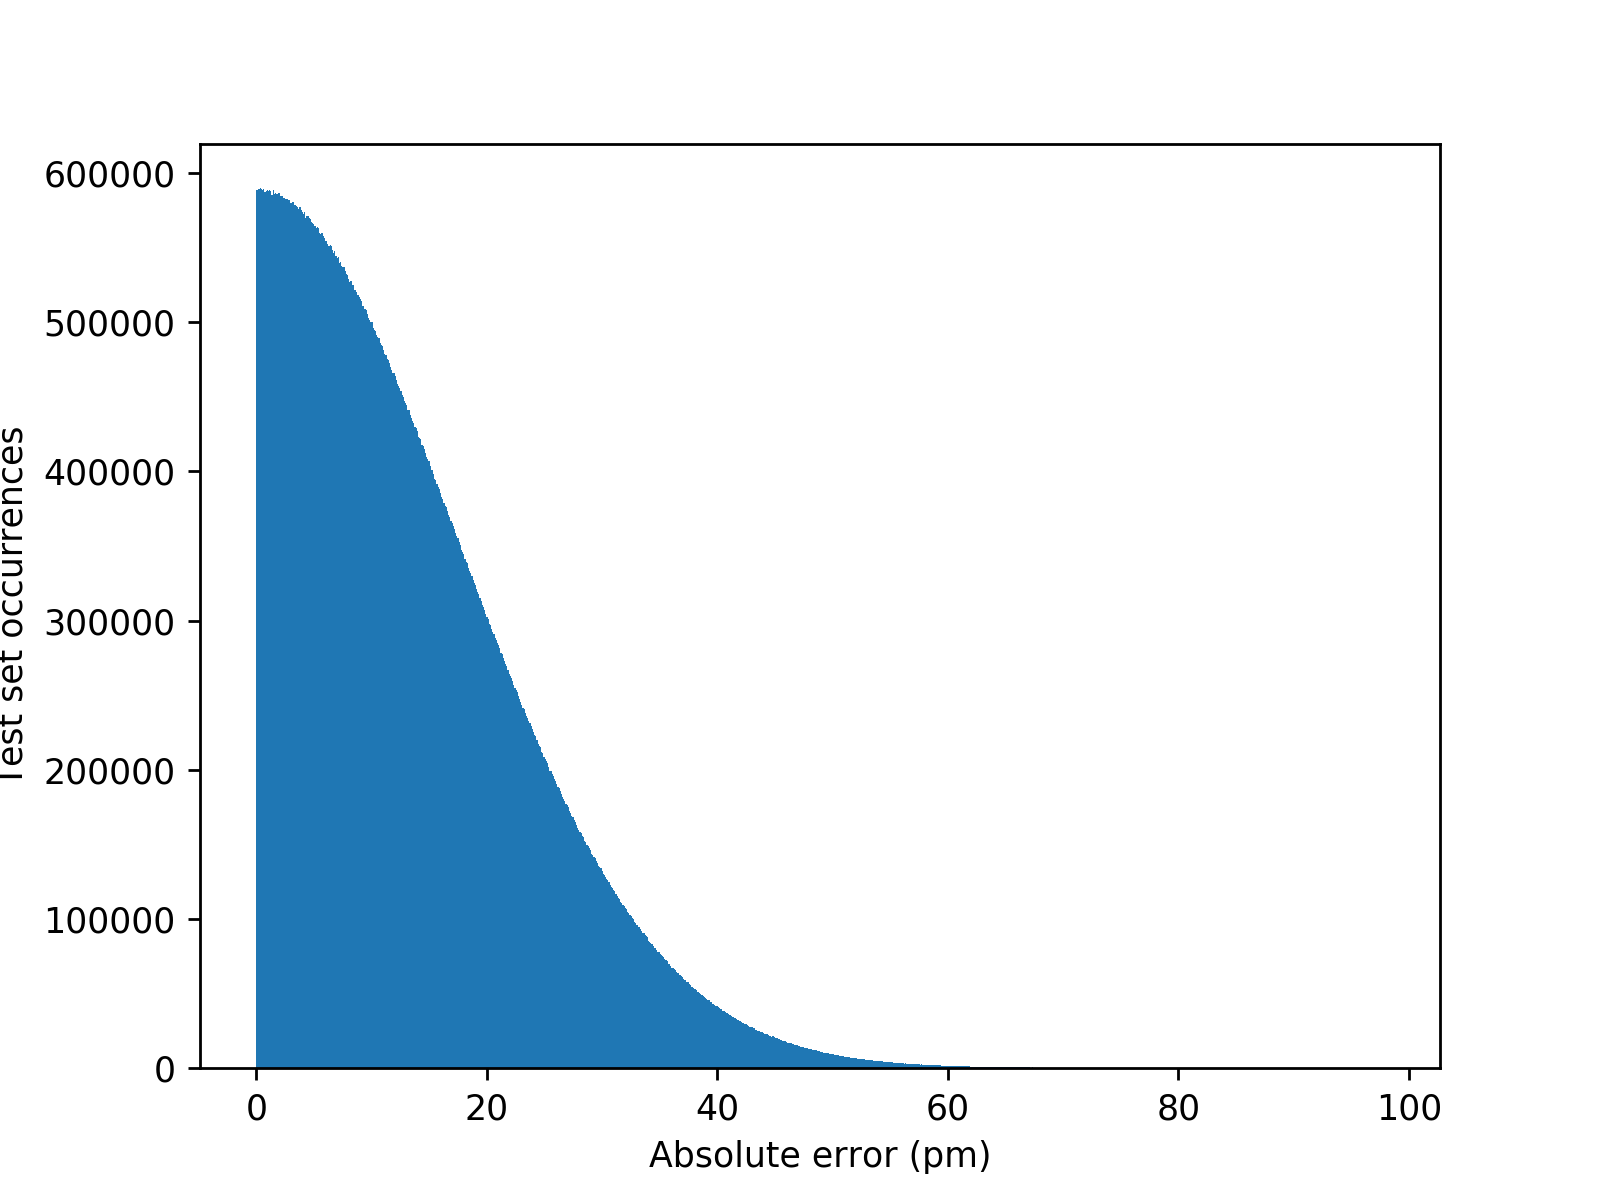
\includegraphics[scale=0.7]{../figures/DELTA_DIST_+H_05/DELTA_DIST+H_05_distrib_rmse_val.png}	
	
	\caption{Distribution des erreurs du modèle \emph{DELTA\_DIST\_+H\_05}}
\end{figure}

L'erreur semble suivre une distribution gaussienne. L'erreur présentée ici étant l'erreur absolue, nous ne voyons qu'une demi courbe de Gauss. Cela montre que le bruit a été en partie « absorbé » par la prédiction (37\%, REF ESTIM PERF) mais qu'il est resté intact.

\subsubsection{Distribution de l'erreur absolue en fonction des cibles}

La représentation de la distribution de l'erreur absolue en fonction des cibles montre que la majorité des prédictions sont très proches de zéro, et que les autres sont proches de -9. Il s'agit probablement d'une méthode pour le modèle de minimiser « en moyenne » la fonction de coût. Les prédictions autour de -9 font probablement partie des raisons pour laquelle la fonction de coût diminue de 37\% par rapport à l'erreur introduite par le bruit. Le modèle semble en effet ici apprendre une règle d'ordre géométrique qui lui permet de minimiser l'erreur dans certains cas.


\begin{figure}[!h]
	\centering
	
	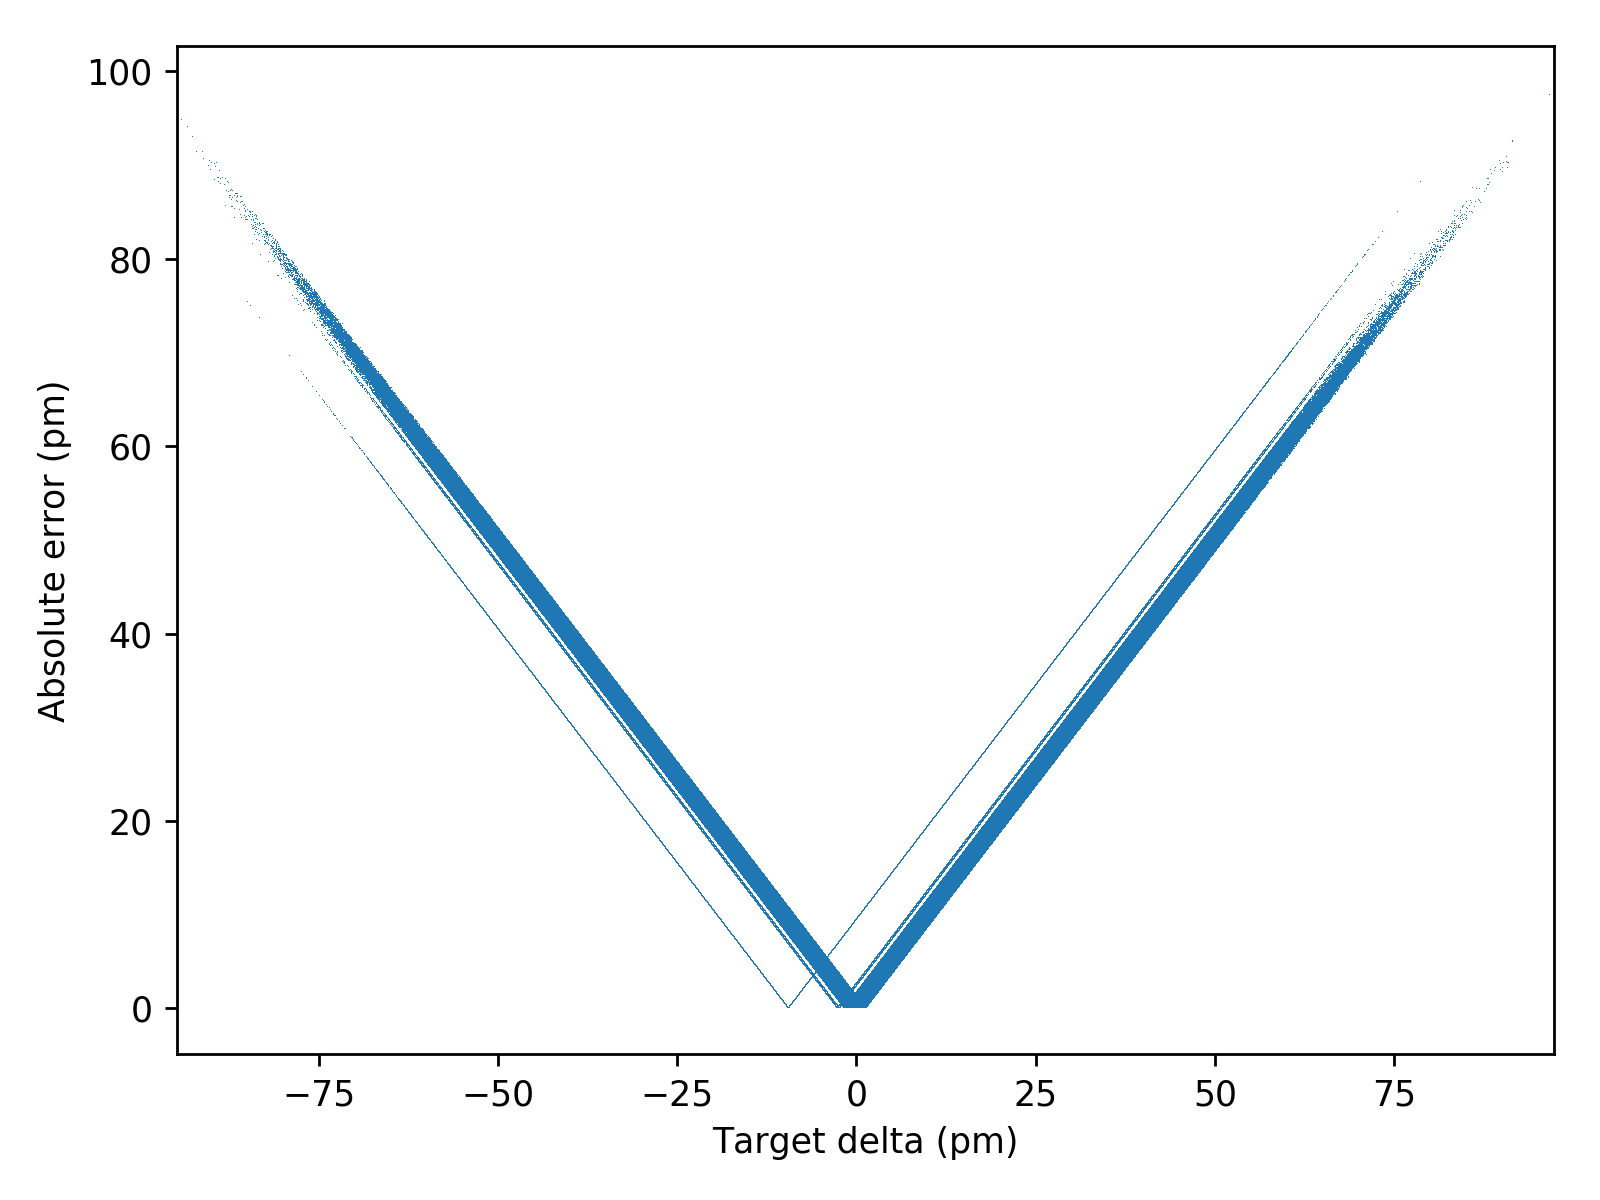
\includegraphics[scale=0.7]{../figures/DELTA_DIST_+H_05/DELTA_DIST+H_05_distrib_rmse_dist.png}	
	
	\caption{Erreur en fonction des cibles pour le modèle \emph{DELTA\_DIST\_+H\_05}}
	\end{figure}



\subsubsection{Distribution des prédictions en fonctions des cibles}

\begin{figure}[!h]
	\centering
	
	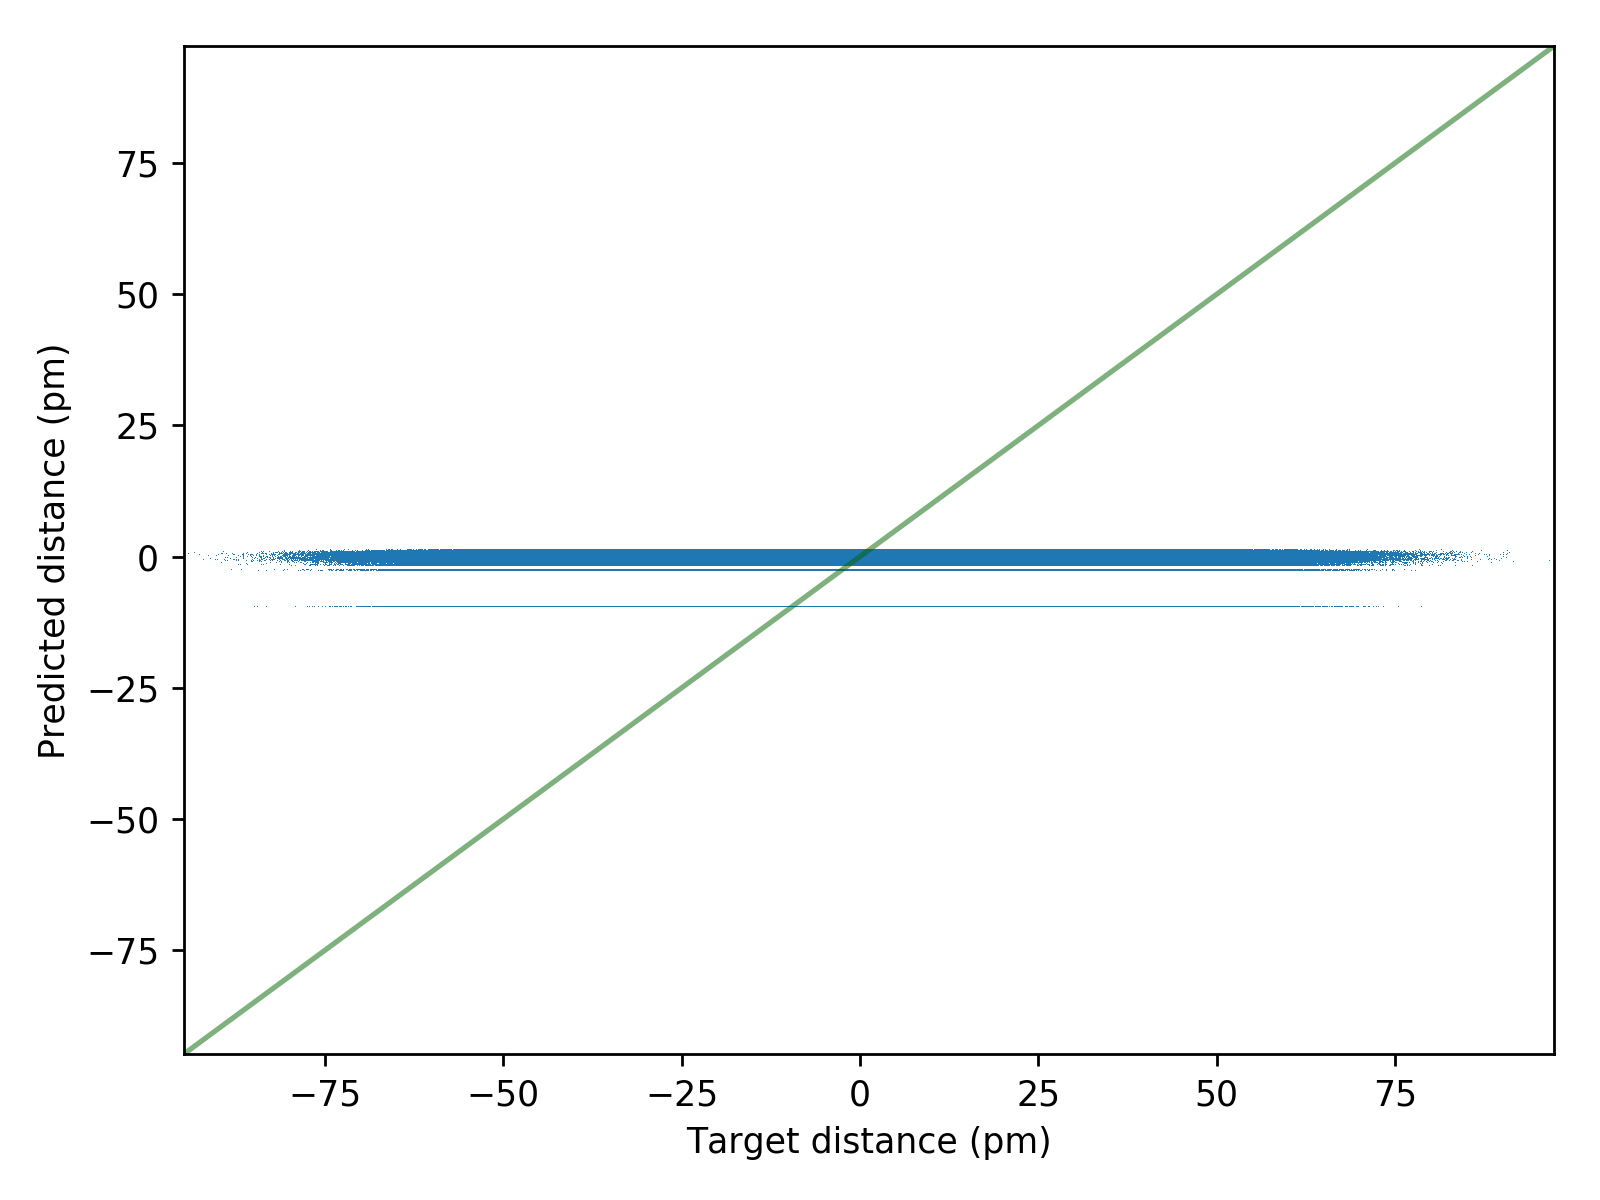
\includegraphics[scale=0.7]{../figures/DELTA_DIST_+H_05/DELTA_DIST+H_05_preds_targets.png}	
	
	\caption{Prédictions en fonction des cibles pour le modèle \emph{DELTA\_DIST\_+H\_05}}
	
\end{figure}

\par La droite tracée correspond aux valeurs attendues. Les prédictions du modèle ont une intersection avec la droite limitée aux prédictions proches de zéro et de -9.

\begin{figure}[!h]
	\centering
	
	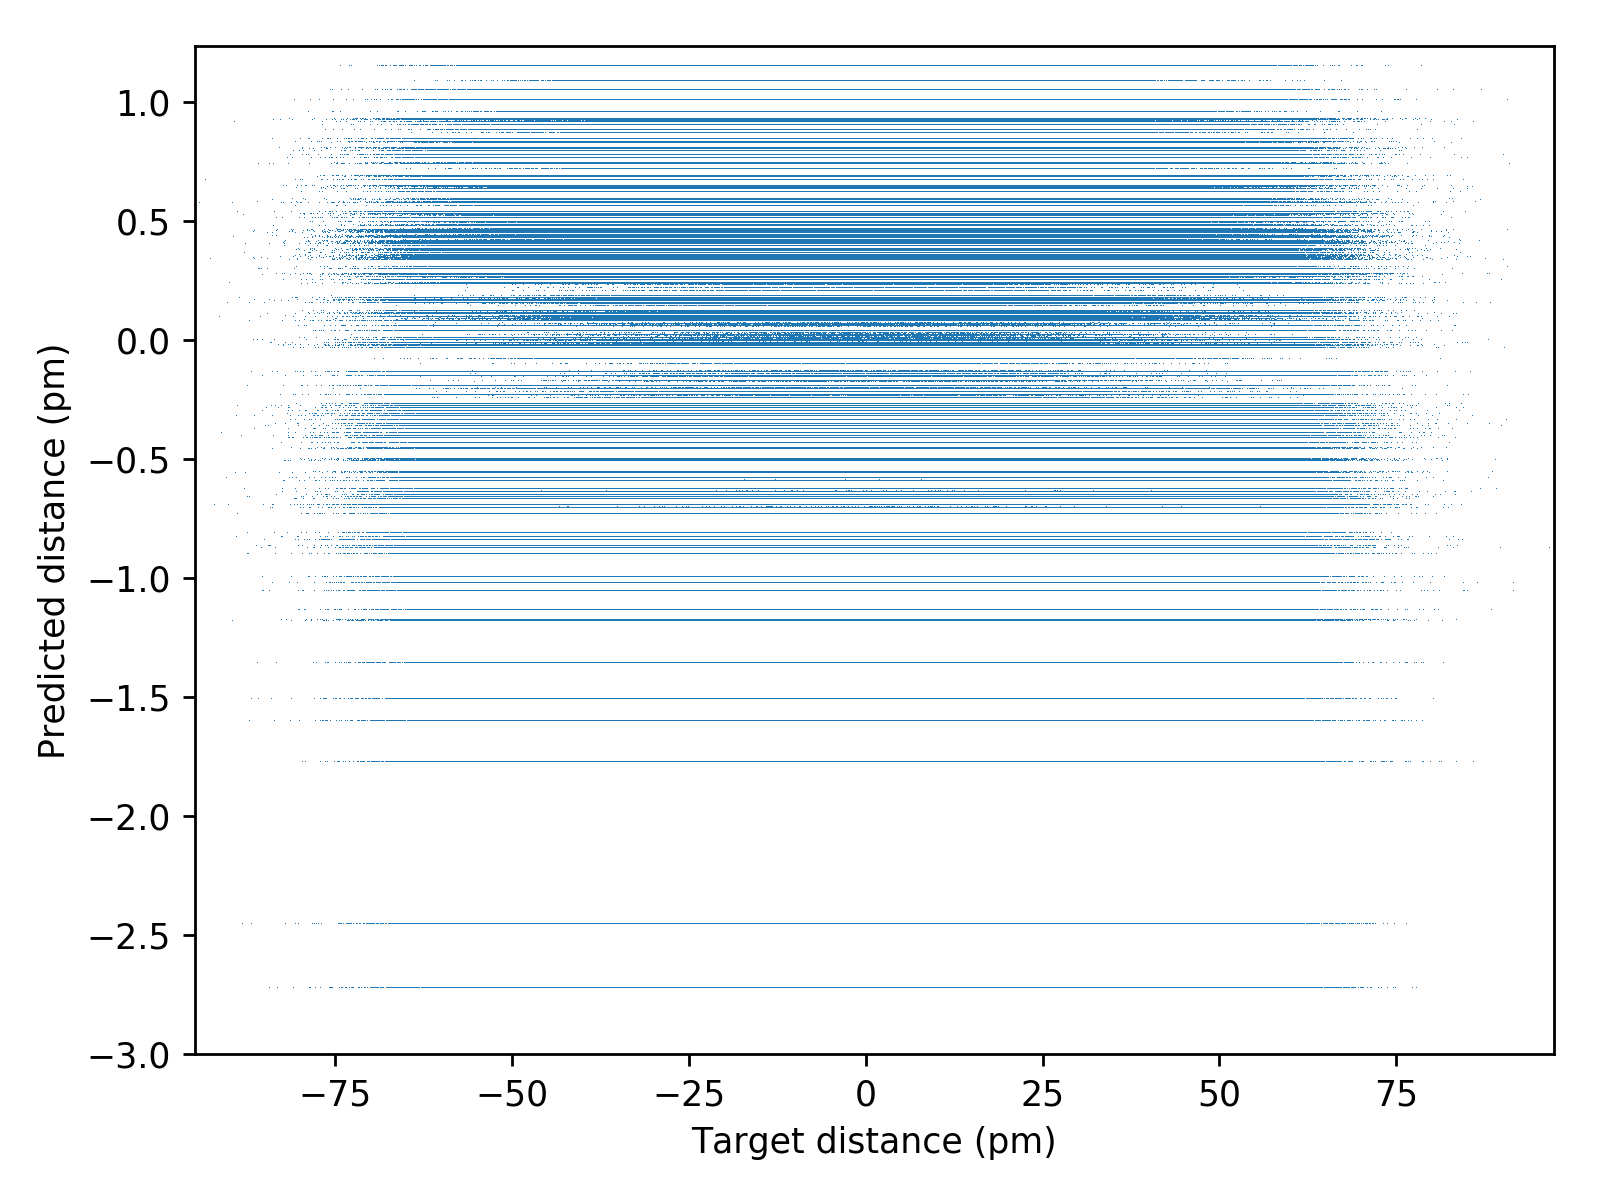
\includegraphics[scale=0.7]{../figures/DELTA_DIST_+H_05/DELTA_DIST+H_05_preds_targets_zoom.png}	
	
	\caption{Prédictions en fonction des cibles pour le modèle \emph{DELTA\_DIST\_+H\_05} (zoom)}
	
\end{figure}
\par Lorsque l'on regarde de plus près les prédictions, on s'aperçoit qu'elles prennent des valeurs discrètes. Cette subtilité peut en partie expliquer la capacité du modèle à prédire partiellement le bruit.

\subsection{Abandon de la méthode}

Le fait que le modèle effectue des prédictions constantes et l'impossibilité de produire de meilleurs résultats à l'issue de la recherche par quadrillage (REF QUADRI) ont mené à l'abandon de la méthode pour prédire des géométries moléculaires convergées, au profit d'une méthode moins ambitieuse (REF DIST REL).\\

\par Il est démontré qu'il existe une fonction permettant d'optimiser la géométrie moléculaire, et que les réseaux de neurones sont des approximateurs universels de fonctions\cite{universal_approx}. La tâche que nous avons tenté d'accomplir avec ces modèles est donc théoriquement possible. Nous pouvons toutefois trouver quelques explications possibles à notre incapacité à entraîner un modèle suffisamment efficace. 

\par Premièrement, les modèles que nous avons entraînés sont des modèles aux architectures relativement simples, avec un nombre de neurones et de connexions limité par les capacités matérielles. Des architectures plus complexes auraient pu mener à de meilleures performances pour les mêmes données. \\
Un autre écueil pourrait être le manque de données. Même si nous travaillons sur un jeu de données contenant 3,7 millions de molécules (REF DONNES), il s'agit peut-être d'une quantité insuffisante pour approximer correctement une fonction aussi complexe. De même, il est possible qu'il manque certains descripteurs des molécules en entrée des modèles.\\
Enfin, il est possible que le problème soit lié à notre méthodologie, et notamment au fait que l'on génère un jeu d'entraînement en ajoutant du bruit sur les données à prédire. Peut-être la tâche de prédiction est-elle impossible à réaliser à cause du caractère aléatoire et par définition imprédictible du bruit gaussien, même si on peut raisonnablement imaginer que si un modèle est capable de prédire une géométrie convergée, il est capable de soustraire la géométrie convergée d'une géométrie bruitée.




\chapter{Conclusion}
	\addcontentsline{toc}{chapter}{Conclusion}  



	\begin{thebibliography}{9}

	\bibitem{tf}
		Martín Abadi, Ashish Agarwal, Paul Barham, Eugene Brevdo,
Zhifeng Chen, Craig Citro, Greg S. Corrado, Andy Davis,
Jeffrey Dean, Matthieu Devin, Sanjay Ghemawat, Ian Goodfellow,
Andrew Harp, Geoffrey Irving, Michael Isard, Rafal Jozefowicz, Yangqing Jia,
Lukasz Kaiser, Manjunath Kudlur, Josh Levenberg, Dan Mané, Mike Schuster,
Rajat Monga, Sherry Moore, Derek Murray, Chris Olah, Jonathon Shlens,
Benoit Steiner, Ilya Sutskever, Kunal Talwar, Paul Tucker,
Vincent Vanhoucke, Vijay Vasudevan, Fernanda Viégas,
Oriol Vinyals, Pete Warden, Martin Wattenberg, Martin Wicke,
Yuan Yu, and Xiaoqiang Zheng.
TensorFlow: Large-scale machine learning on heterogeneous systems,
2015. Software available from tensorflow.org.

	\bibitem{jupyter}
		Kluyver, Thomas, Ragan-Kelley, Benjamin, Pérez, Fernando, Granger, Brian, Bussonnier, Matthias, Frederic, Jonathan, Kelley, Kyle, Hamrick, Jessica, Grout, Jason, Corlay, Sylvain, Ivanov, Paul, Avila, Damián, Abdalla, Safia, Willing, Carol and [Unknown], Jupyter development team (2016) Jupyter Notebooks – a publishing format for reproducible computational workflows. Loizides, Fernando and Scmidt, Birgit (eds.) In Positioning and Power in Academic Publishing: Players, Agents and Agendas. IOS Press. pp. 87-90. (doi:10.3233/978-1-61499-649-1-87).
		
	\bibitem{adam}
		arXiv:1412.6980 


	\bibitem{weight_decay}
	Krogh, Anders \& Hertz, J. (1992). A Simple Weight Decay Can Improve Generalization. Adv. Neural Inform. Process Systems. 4. 

	\bibitem{pubchem}
		Kim S, Thiessen PA, Bolton EE, Chen J, Fu G, Gindulyte A, Han L, He J, He S, Shoemaker BA, Wang J, Yu B, Zhang J, Bryant SH. PubChem Substance and Compound databases. Nucleic Acids Res. 2016 Jan 4; 44(D1):D1202-13. Epub 2015 Sep 22 [PubMed PMID: 26400175] doi: 10.1093/nar/gkv951
		
	\bibitem{gdb}
		J. Chem. Inf. Model.  52, 11, 2864-2875		

	\bibitem{pubchemqc}
		J. Chem. Inf. Model.  57, 6, 1300-1308

	\bibitem{sklearn}
		Scikit-learn: Machine Learning in Python, Pedregosa et al., JMLR 12, pp. 2825-2830, 2011

	\bibitem{universal_approx}
		K. Hornik, M. Stinchcombe, and H. White, Multi-layer feedforward networks are universal 	approximators, preprint, 1988. 
		
	\bibitem{mg} Kearnes, S., McCloskey, K., Berndl, M., Pande, V., \& Riley, P.\ 2016, Journal of Computer-Aided Molecular Design, 30, 595 
	
	\bibitem{jctc_prediction}
		J. Chem. Theory Comput.  13, 11, 5255-5264
	
	\bibitem{rdkit} RDKit : Open-source cheminformatics. www.rkdit.org. [accessed 11-April-2013]
	
	\bibitem{graph_fingerprint}
		arXiv:1509.09292 [cs.LG]
	
	

	
          
\end{thebibliography}



\addappheadtotoc
\appendixpage

\appendix

\begin{landscape}


\chapter{Diagramme de Gantt}
\label{gantt}
\begin{figure}[!h]
	\centering

	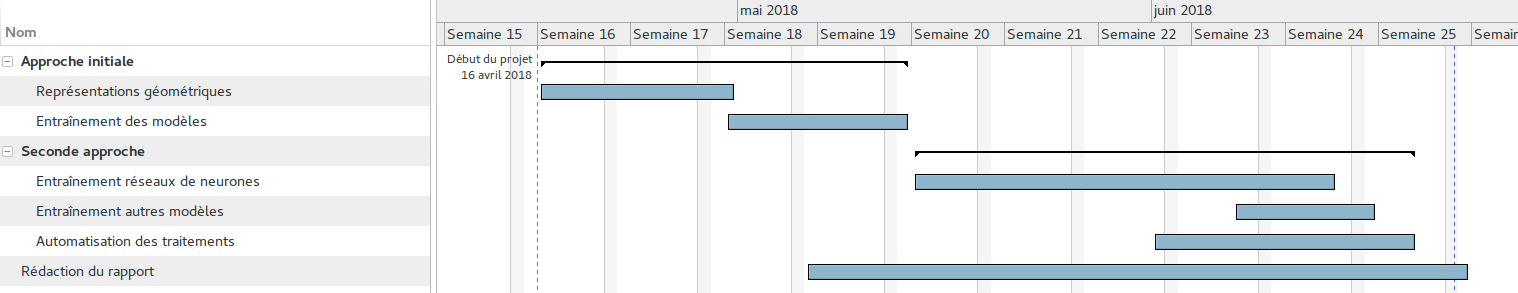
\includegraphics[scale=0.45]{images/gantt.png}	
	
	\caption{Diagramme de Gantt des grandes étapes du travail (Généré avec le programme Planner)}
\end{figure}

\end{landscape}


\chapter{Représentations graphiques des prédictions des modèles \emph{DIST\_REL\_C}}

\label{annexes_plots_dist_rel_c}

\begin{figure}[!h]
	\centering
	
	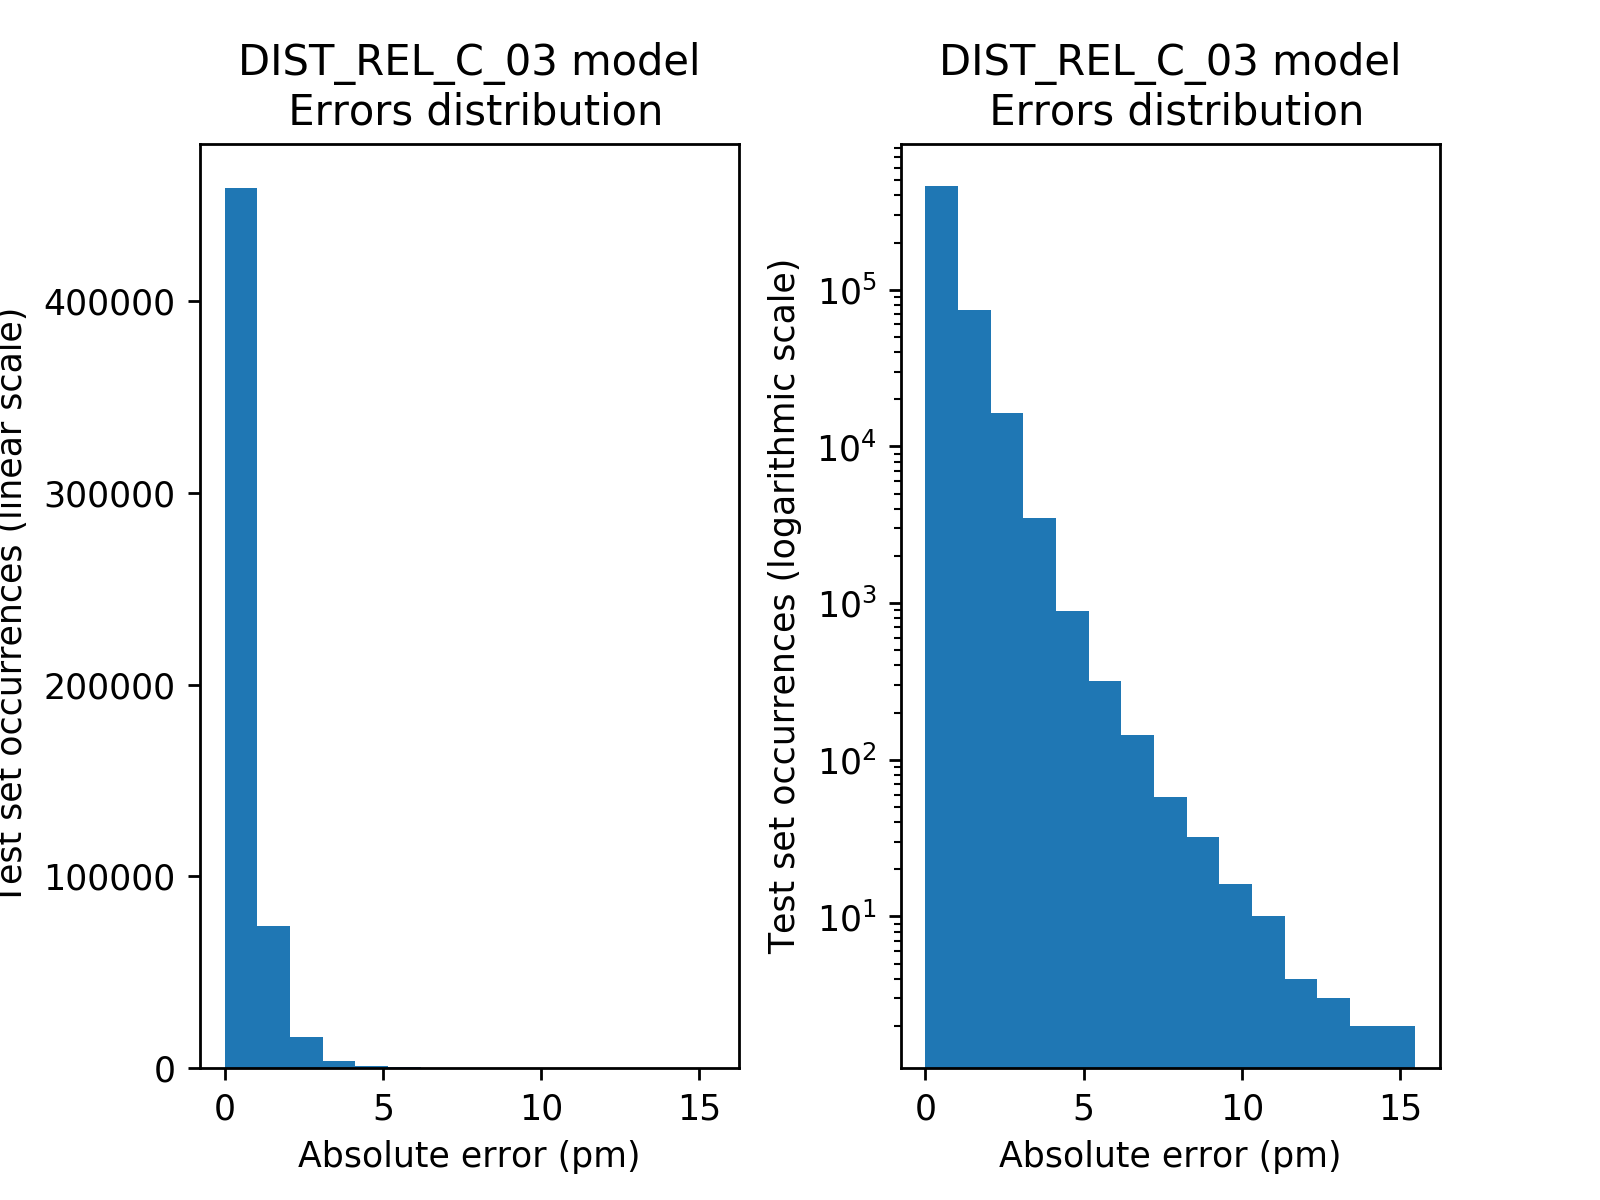
\includegraphics[scale=0.75]{../figures/DIST_REL_C_03/DIST_REL_C_03_distrib_rmse_val.png}	
	
	\caption{Distribution des erreurs du modèle \emph{DIST\_REL\_C\_03}. Modèle s'entraînant sur une \textbf{quantité modérée d'exemples} et prédisant les longueurs de liaisons \textbf{carbone-carbone}, à partir de données d'entrées sur lesquelles la \textbf{fonction inverse} a été appliquée aux distances, \textbf{avec restriction} au voisinage le plus proche.}
\end{figure}
\begin{figure}[!h]
	\centering
	
	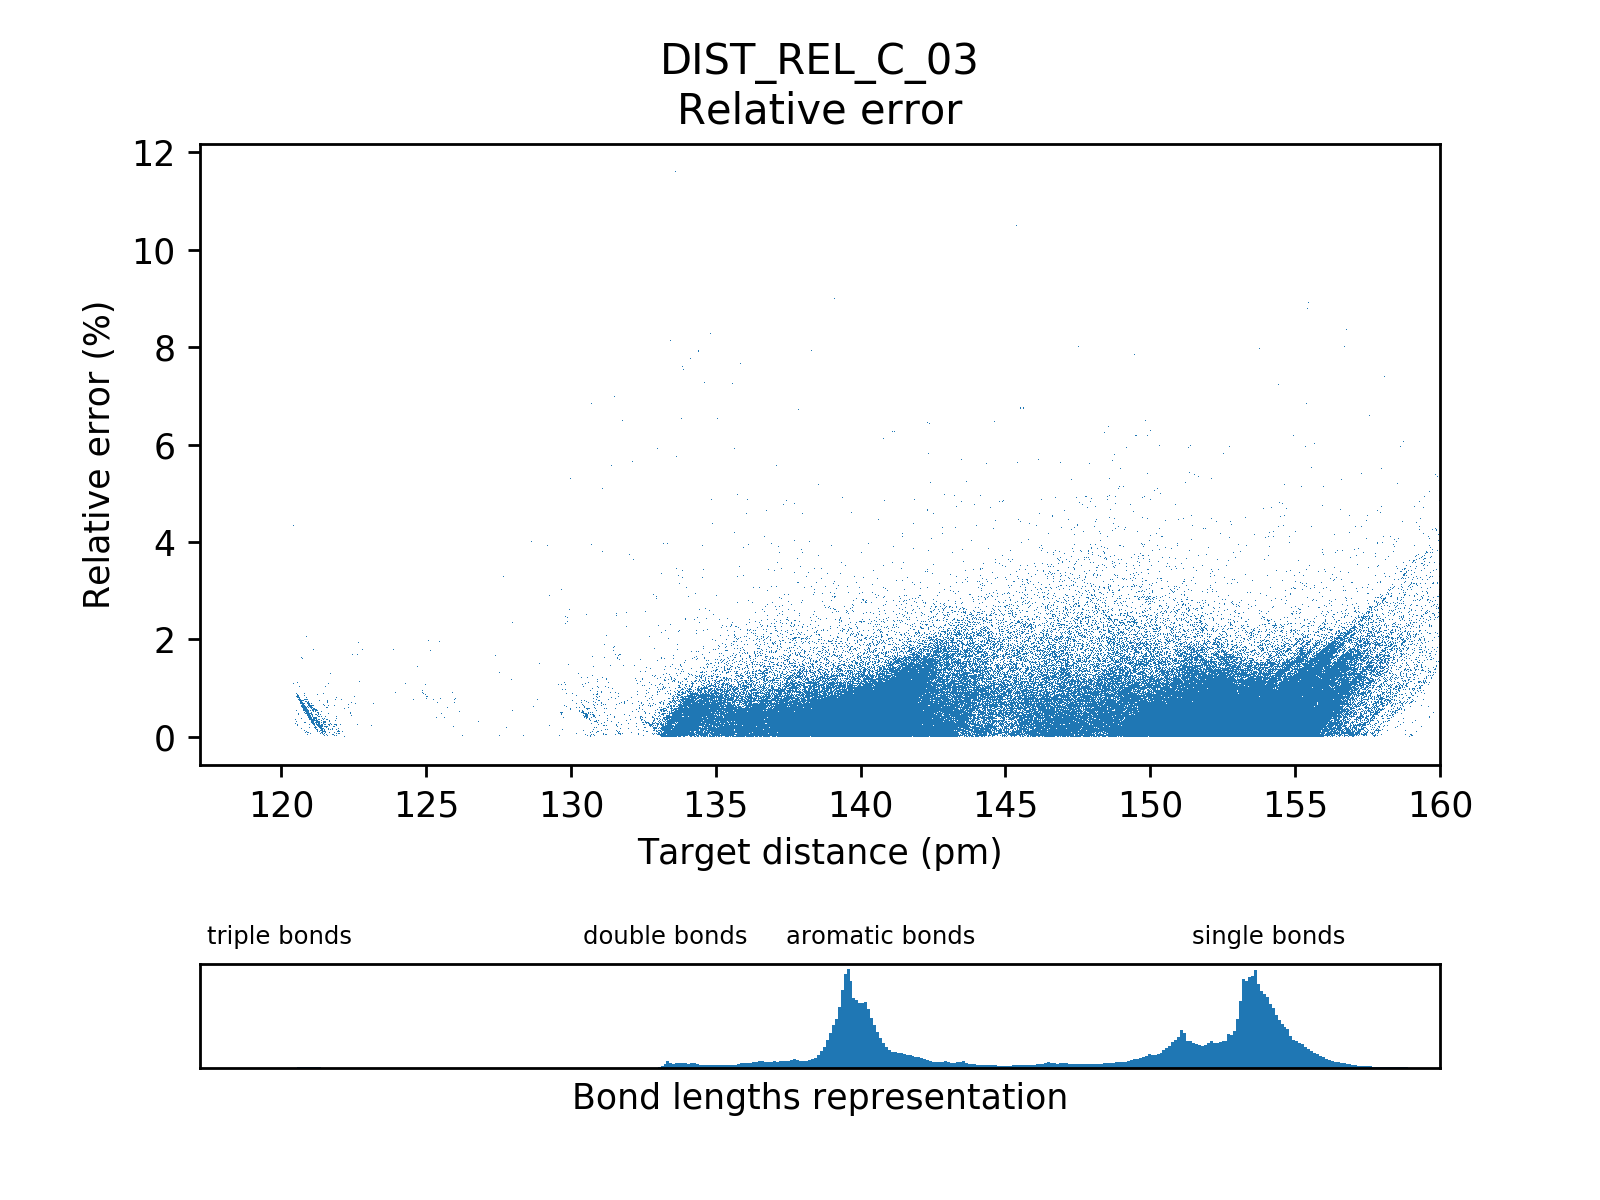
\includegraphics[scale=0.75]{../figures/DIST_REL_C_03/DIST_REL_C_03_distrib_rmse_dist.png}	
	
	\caption{Erreur en fonction des cibles pour le modèle \emph{DIST\_REL\_C\_03}. Modèle s'entraînant sur une \textbf{quantité modérée d'exemples} et prédisant les longueurs de liaisons \textbf{carbone-carbone}, à partir de données d'entrées sur lesquelles la \textbf{fonction inverse} a été appliquée aux distances, \textbf{avec restriction} au voisinage le plus proche.}
	\end{figure}

\begin{figure}[!h]
	\centering
	
	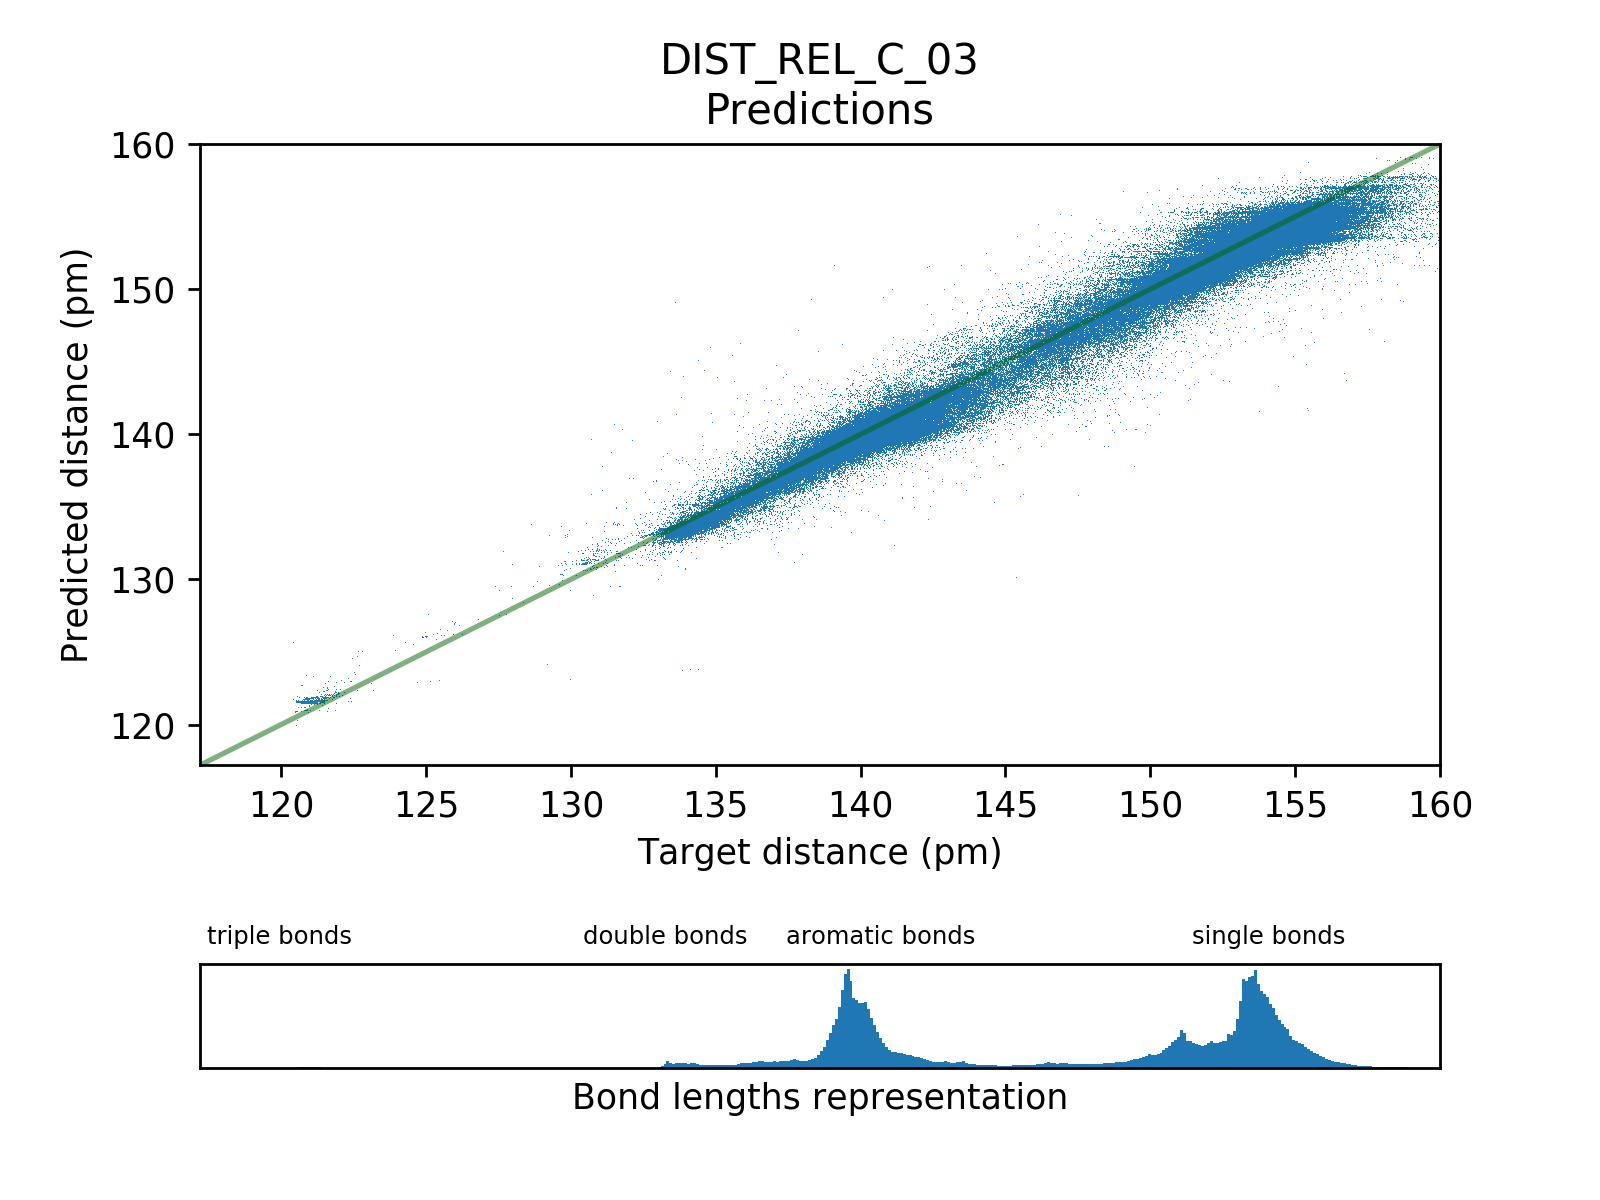
\includegraphics[scale=0.75]{../figures/DIST_REL_C_03/DIST_REL_C_03_preds_targets.png}	
	
	\caption{Prédictions en fonction des cibles pour le modèle \emph{DIST\_REL\_C\_03}. Modèle s'entraînant sur une \textbf{quantité modérée d'exemples} et prédisant les longueurs de liaisons \textbf{carbone-carbone}, à partir de données d'entrées sur lesquelles la \textbf{fonction inverse} a été appliquée aux distances, \textbf{avec restriction} au voisinage le plus proche.}
	
\end{figure}

\begin{figure}[!h]
	\centering
	
	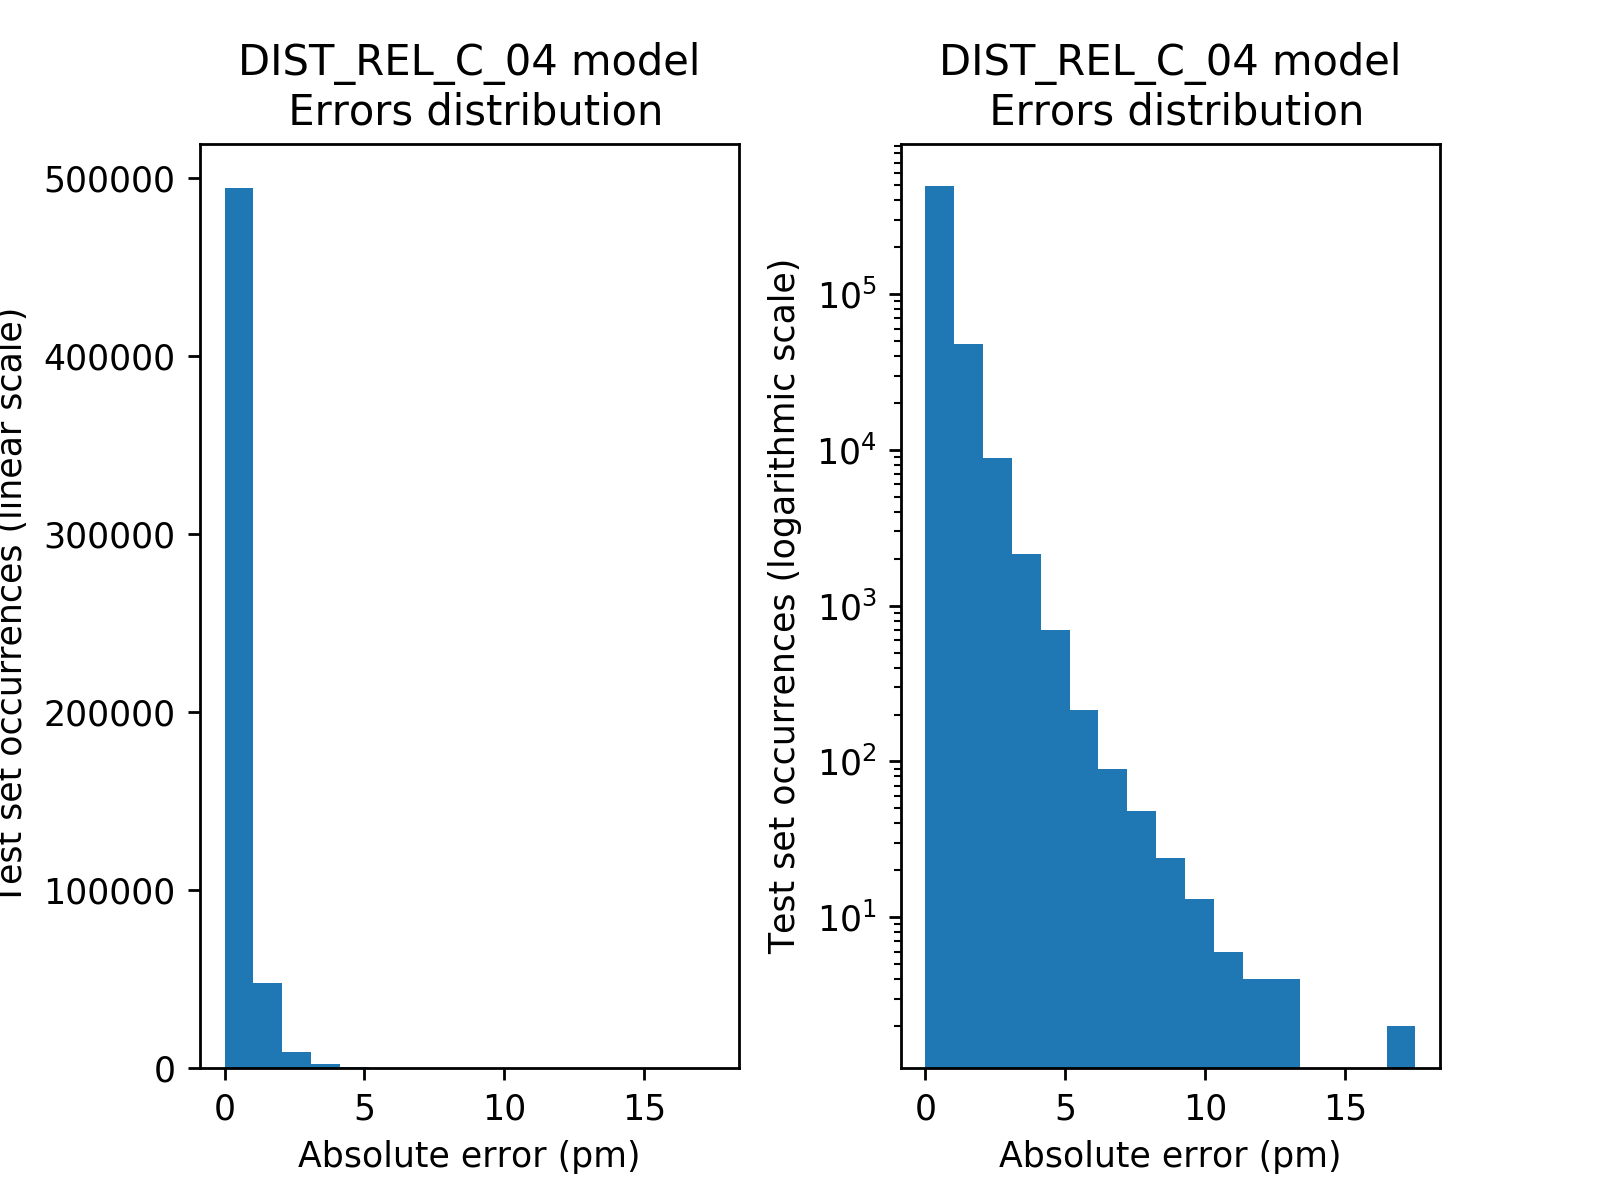
\includegraphics[scale=0.75]{../figures/DIST_REL_C_04/DIST_REL_C_04_distrib_rmse_val.png}	
	
	\caption{Distribution des erreurs du modèle \emph{DIST\_REL\_C\_04}. Modèle s'entraînant sur une \textbf{quantité modérée d'exemples} et prédisant les longueurs de liaisons \textbf{carbone-carbone}, à partir de données d'entrées sur lesquelles la \textbf{fonction inverse du carré} a été appliquée aux distances, \textbf{avec restriction} au voisinage le plus proche.}
\end{figure}
\begin{figure}[!h]
	\centering
	
	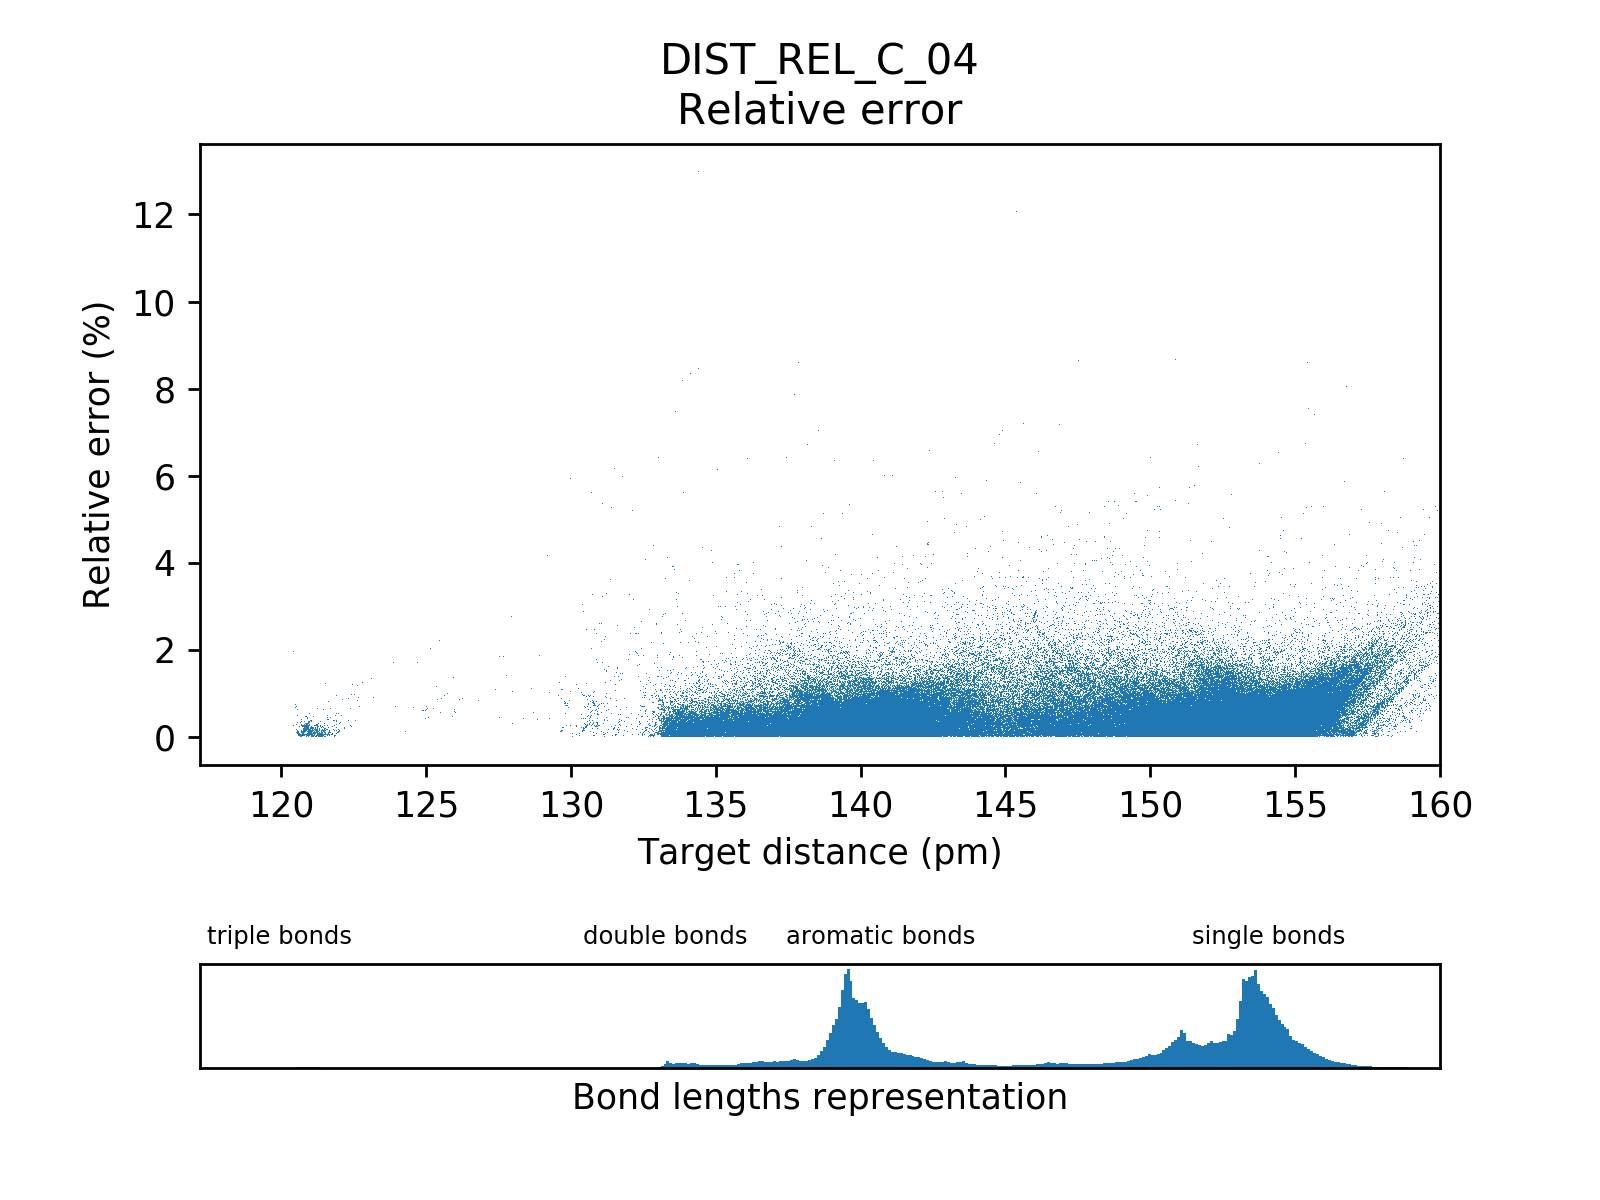
\includegraphics[scale=0.75]{../figures/DIST_REL_C_04/DIST_REL_C_04_distrib_rmse_dist.png}	
	
	\caption{Erreur en fonction des cibles pour le modèle \emph{DIST\_REL\_C\_04}. Modèle s'entraînant sur une \textbf{quantité modérée d'exemples} et prédisant les longueurs de liaisons \textbf{carbone-carbone}, à partir de données d'entrées sur lesquelles la \textbf{fonction inverse du carré} a été appliquée aux distances, \textbf{avec restriction} au voisinage le plus proche.}
	\end{figure}

\begin{figure}[!h]
	\centering
	
	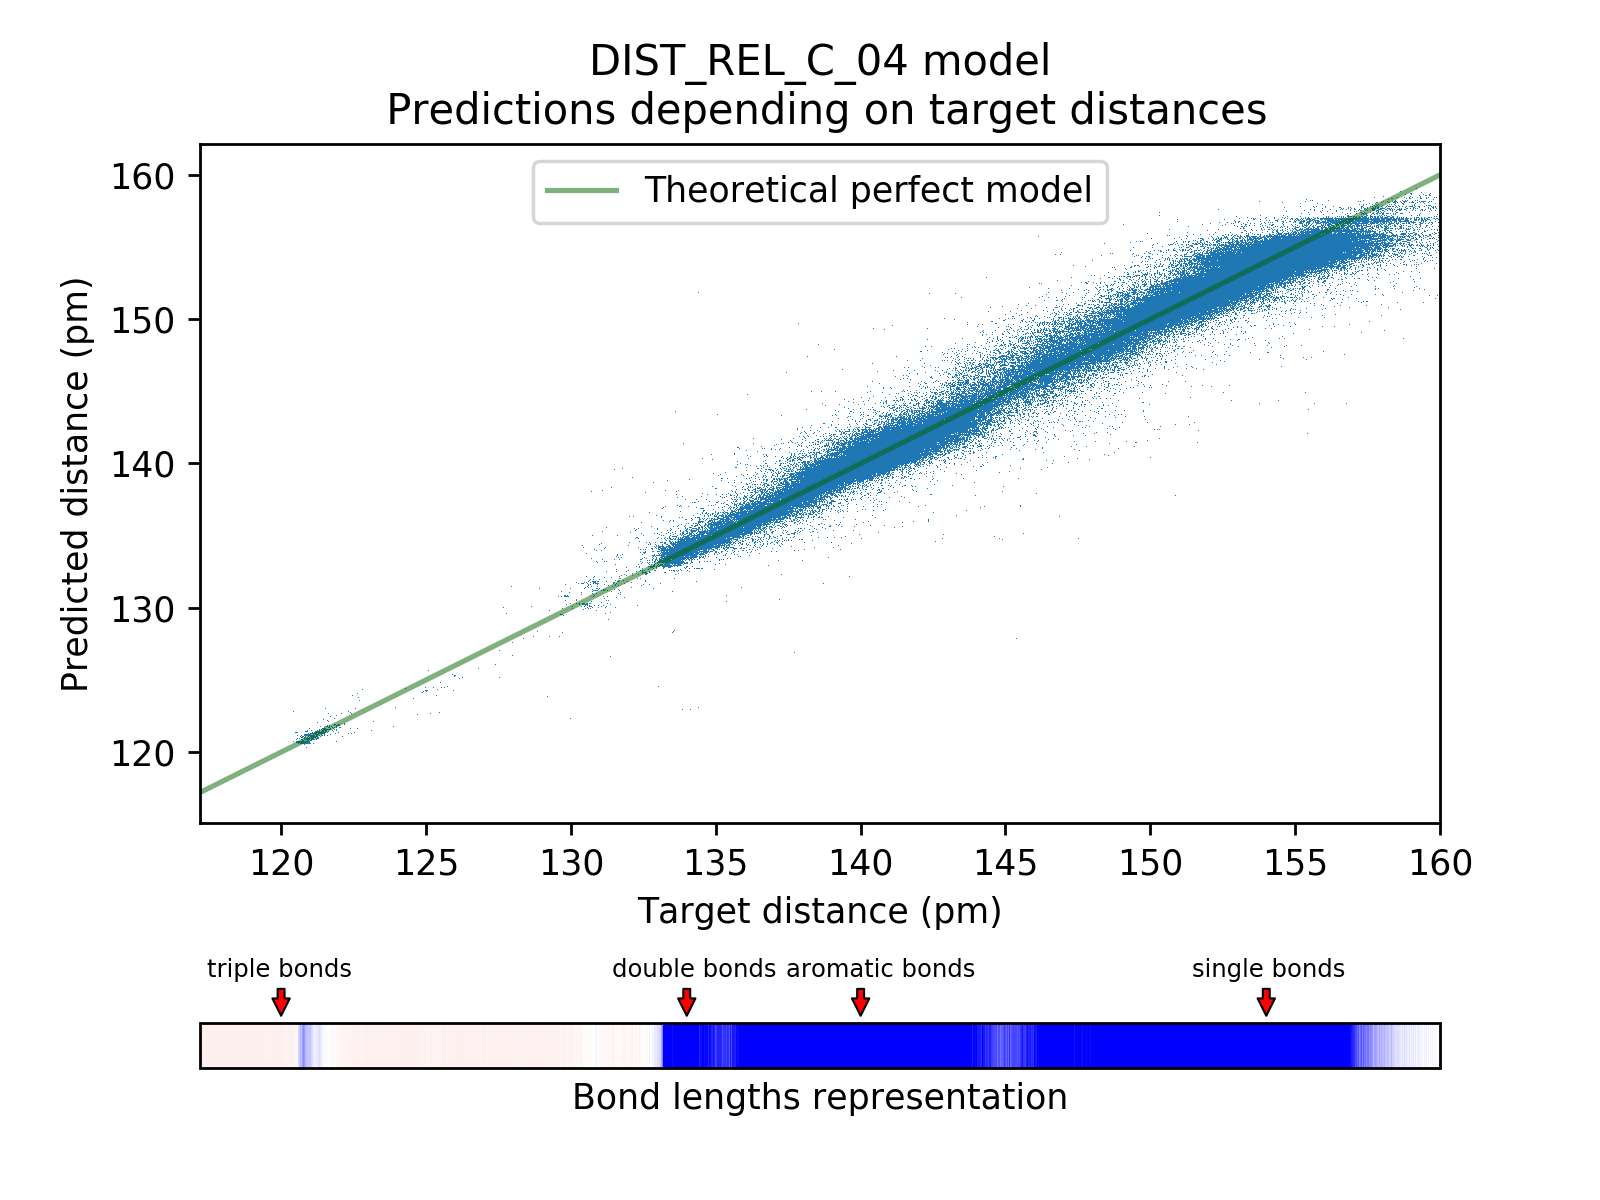
\includegraphics[scale=0.75]{../figures/DIST_REL_C_04/DIST_REL_C_04_preds_targets.png}	
	
	\caption{Prédictions en fonction des cibles pour le modèle \emph{DIST\_REL\_C\_04}. Modèle s'entraînant sur une \textbf{quantité modérée d'exemples} et prédisant les longueurs de liaisons \textbf{carbone-carbone}, à partir de données d'entrées sur lesquelles la \textbf{fonction inverse du carré} a été appliquée aux distances, \textbf{avec restriction} au voisinage le plus proche.}
	
\end{figure}


\chapter{Représentations graphiques des prédictions des modèles \emph{DIST\_REL\_XY}}

\label{annexes_plot_dist_rel_xy}

% DIST REL CC_01
\begin{figure}[!h]
	\centering
	
	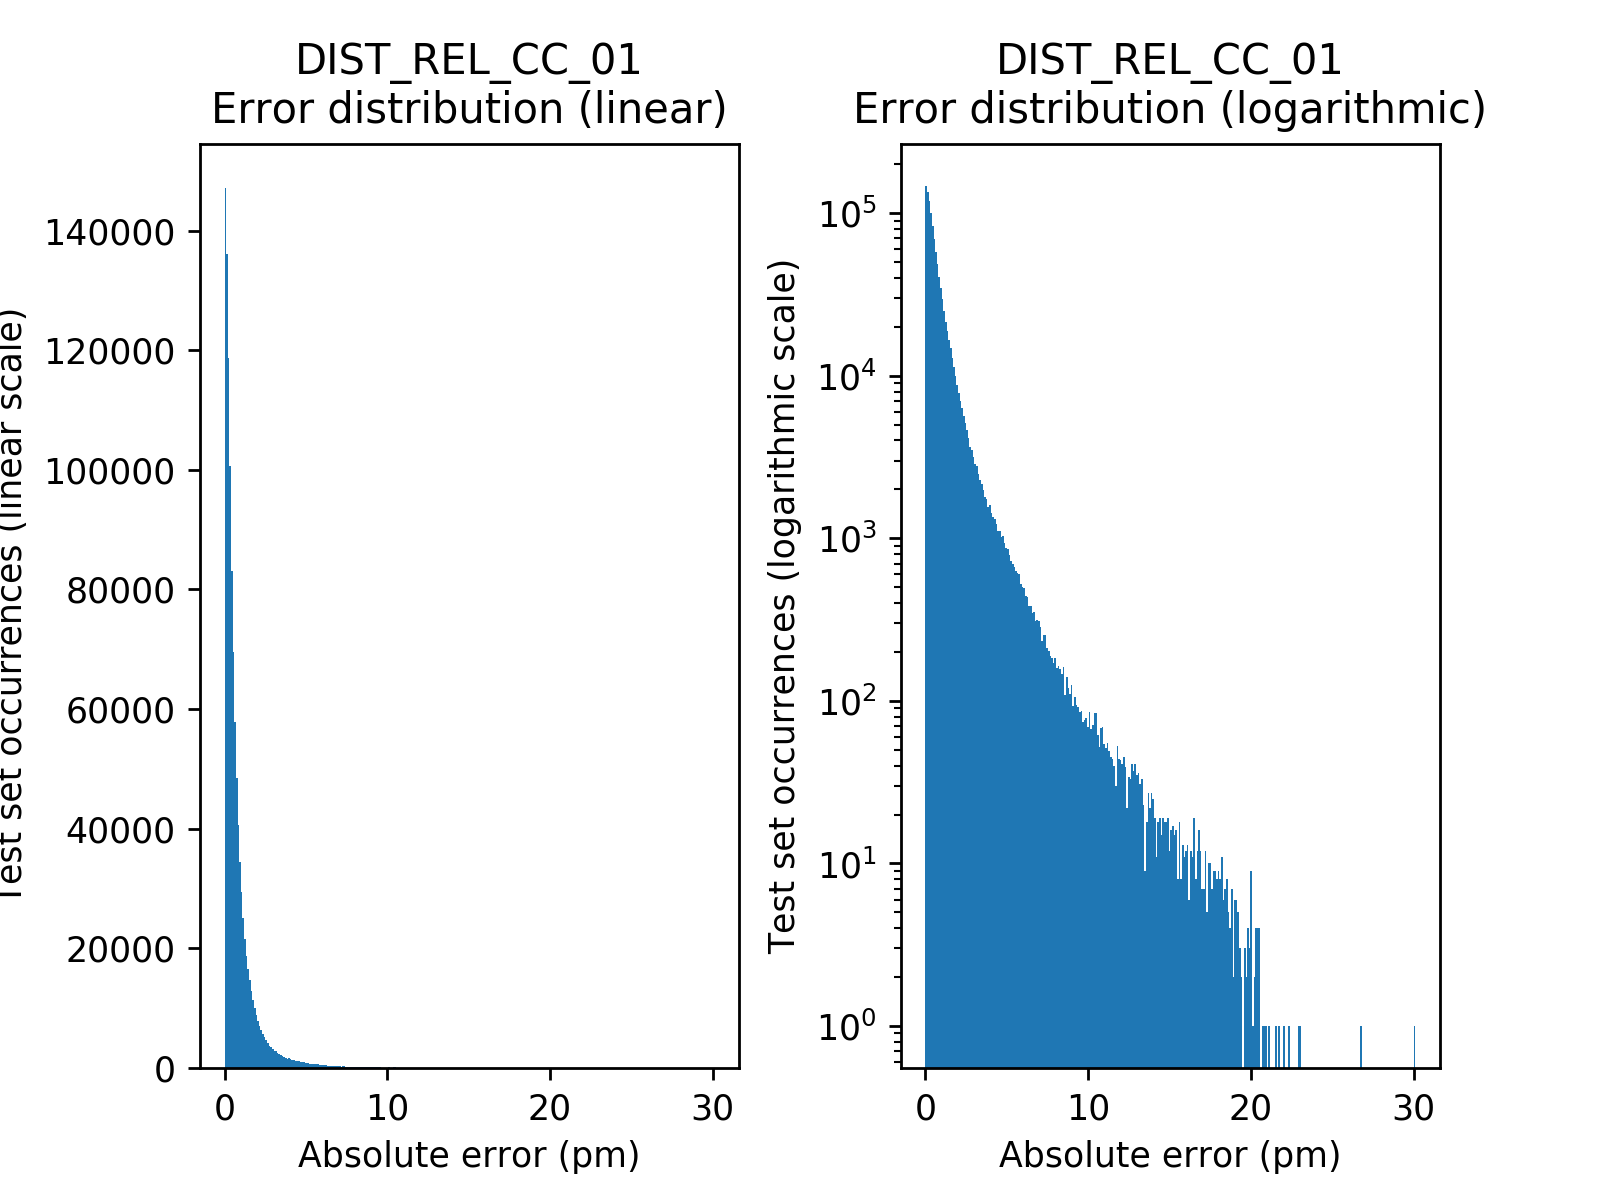
\includegraphics[scale=0.75]{../figures/DIST_REL_CC_01/DIST_REL_CC_01_distrib_rmse_val.png}	
	
	\caption{Distribution des erreurs du modèle \emph{DIST\_REL\_CC\_01}. Modèle s'entraînant sur une \textbf{grande quantité d'exemples} et prédisant les longueurs de liaisons \textbf{carbone-carbone}, à partir de données d'entrées sur lesquelles \textbf{aucune fonction} n'a été appliquée aux distances, \textbf{sans restriction} au voisinage le plus proche.}
\end{figure}
\begin{figure}[!h]
	\centering
	
	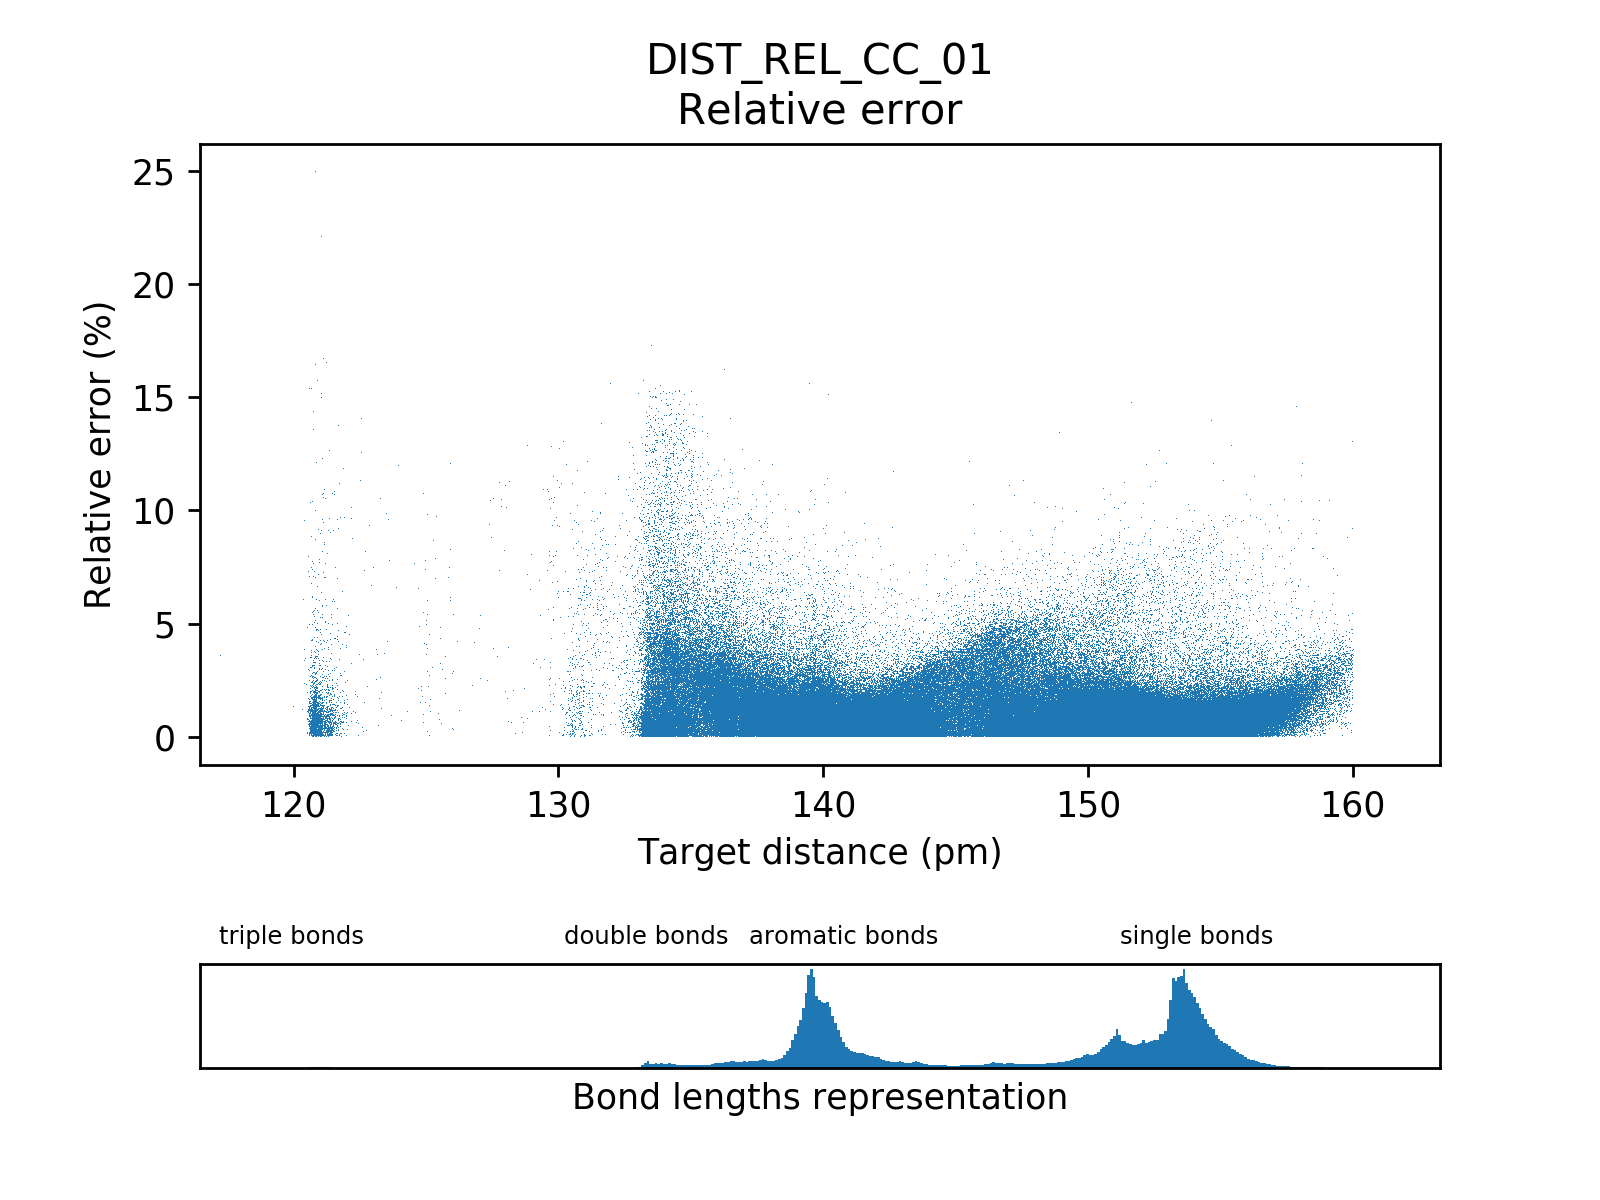
\includegraphics[scale=0.75]{../figures/DIST_REL_CC_01/DIST_REL_CC_01_distrib_rmse_dist.png}	
	
	\caption{Erreur en fonction des cibles pour le modèle \emph{DIST\_REL\_CC\_01}. Modèle s'entraînant sur une \textbf{grande quantité d'exemples} et prédisant les longueurs de liaisons \textbf{carbone-carbone}, à partir de données d'entrées sur lesquelles \textbf{aucune fonction} n'a été appliquée aux distances, \textbf{sans restriction} au voisinage le plus proche.}
	\end{figure}

\begin{figure}[!h]
	\centering
	
	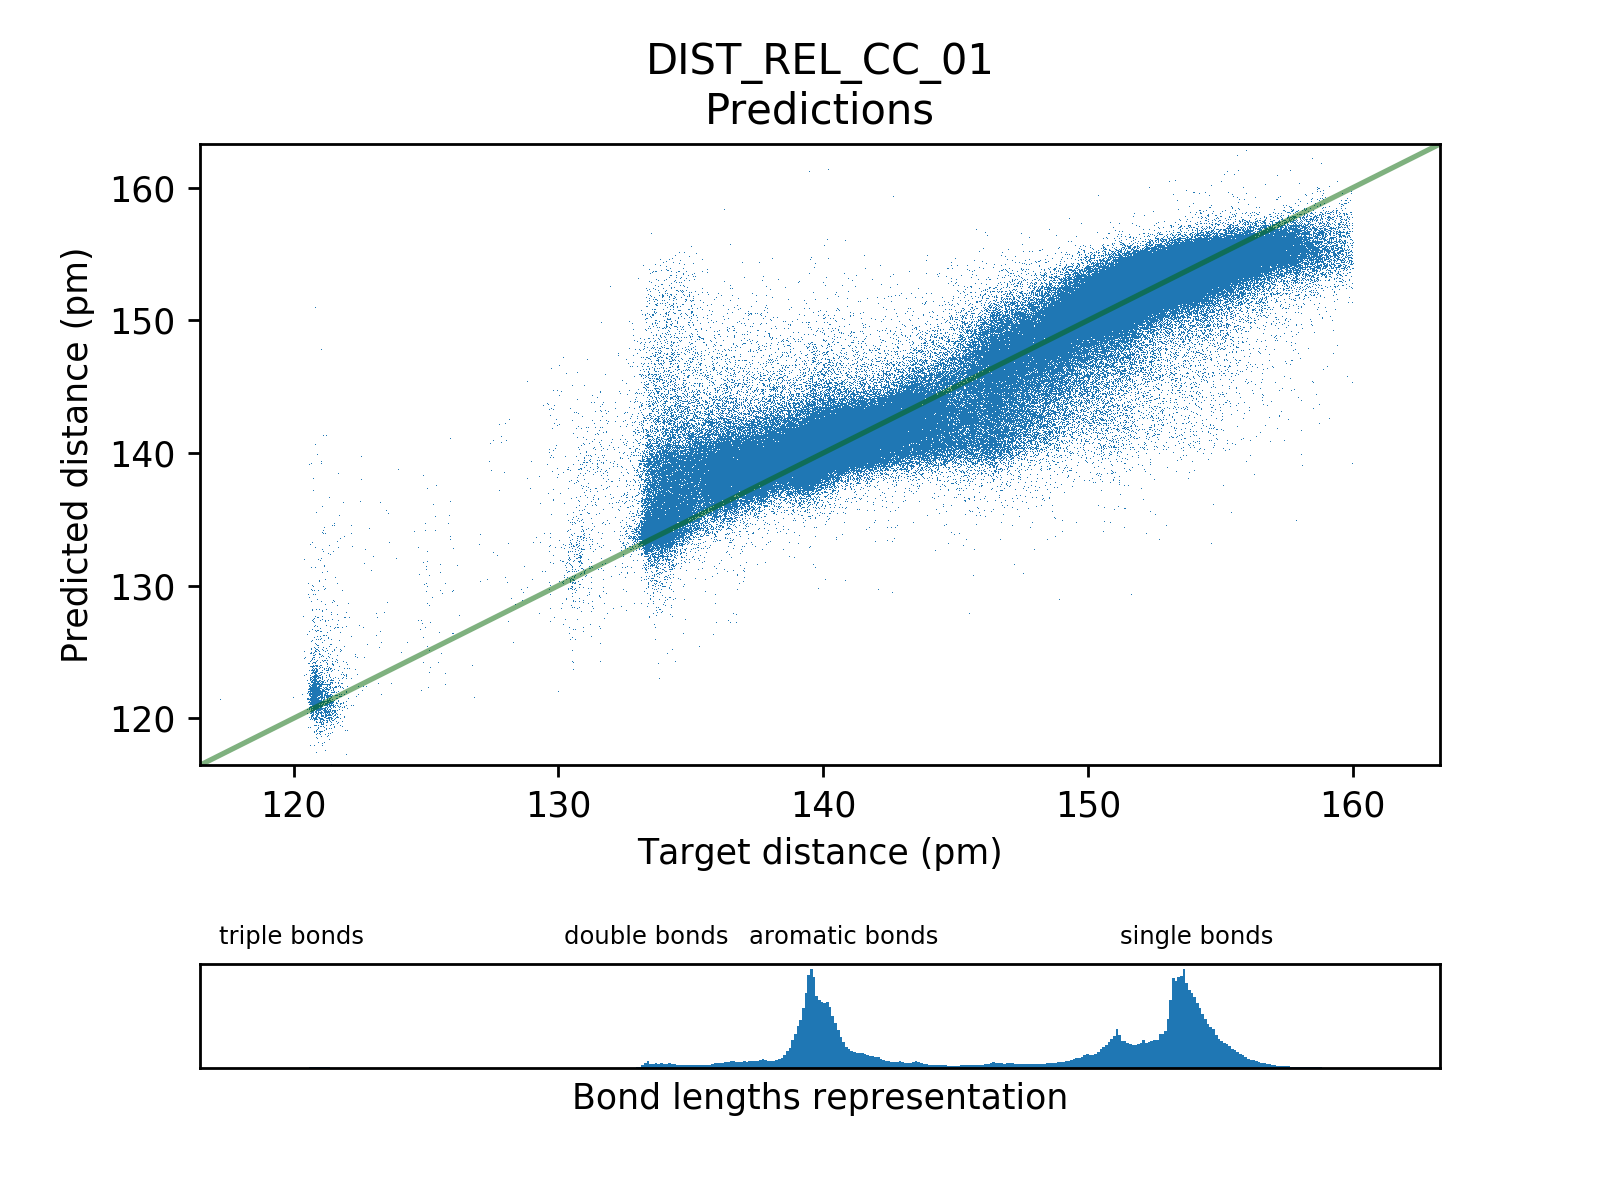
\includegraphics[scale=0.75]{../figures/DIST_REL_CC_01/DIST_REL_CC_01_preds_targets.png}	
	
	\caption{Prédictions en fonction des cibles pour le modèle \emph{DIST\_REL\_CC\_01}. Modèle s'entraînant sur une \textbf{grande quantité d'exemples} et prédisant les longueurs de liaisons \textbf{carbone-carbone}, à partir de données d'entrées sur lesquelles \textbf{aucune fonction} n'a été appliquée aux distances, \textbf{sans restriction} au voisinage le plus proche.}
	
\end{figure}


% DIST REL OH_02

\begin{figure}[!h]
	\centering
	
	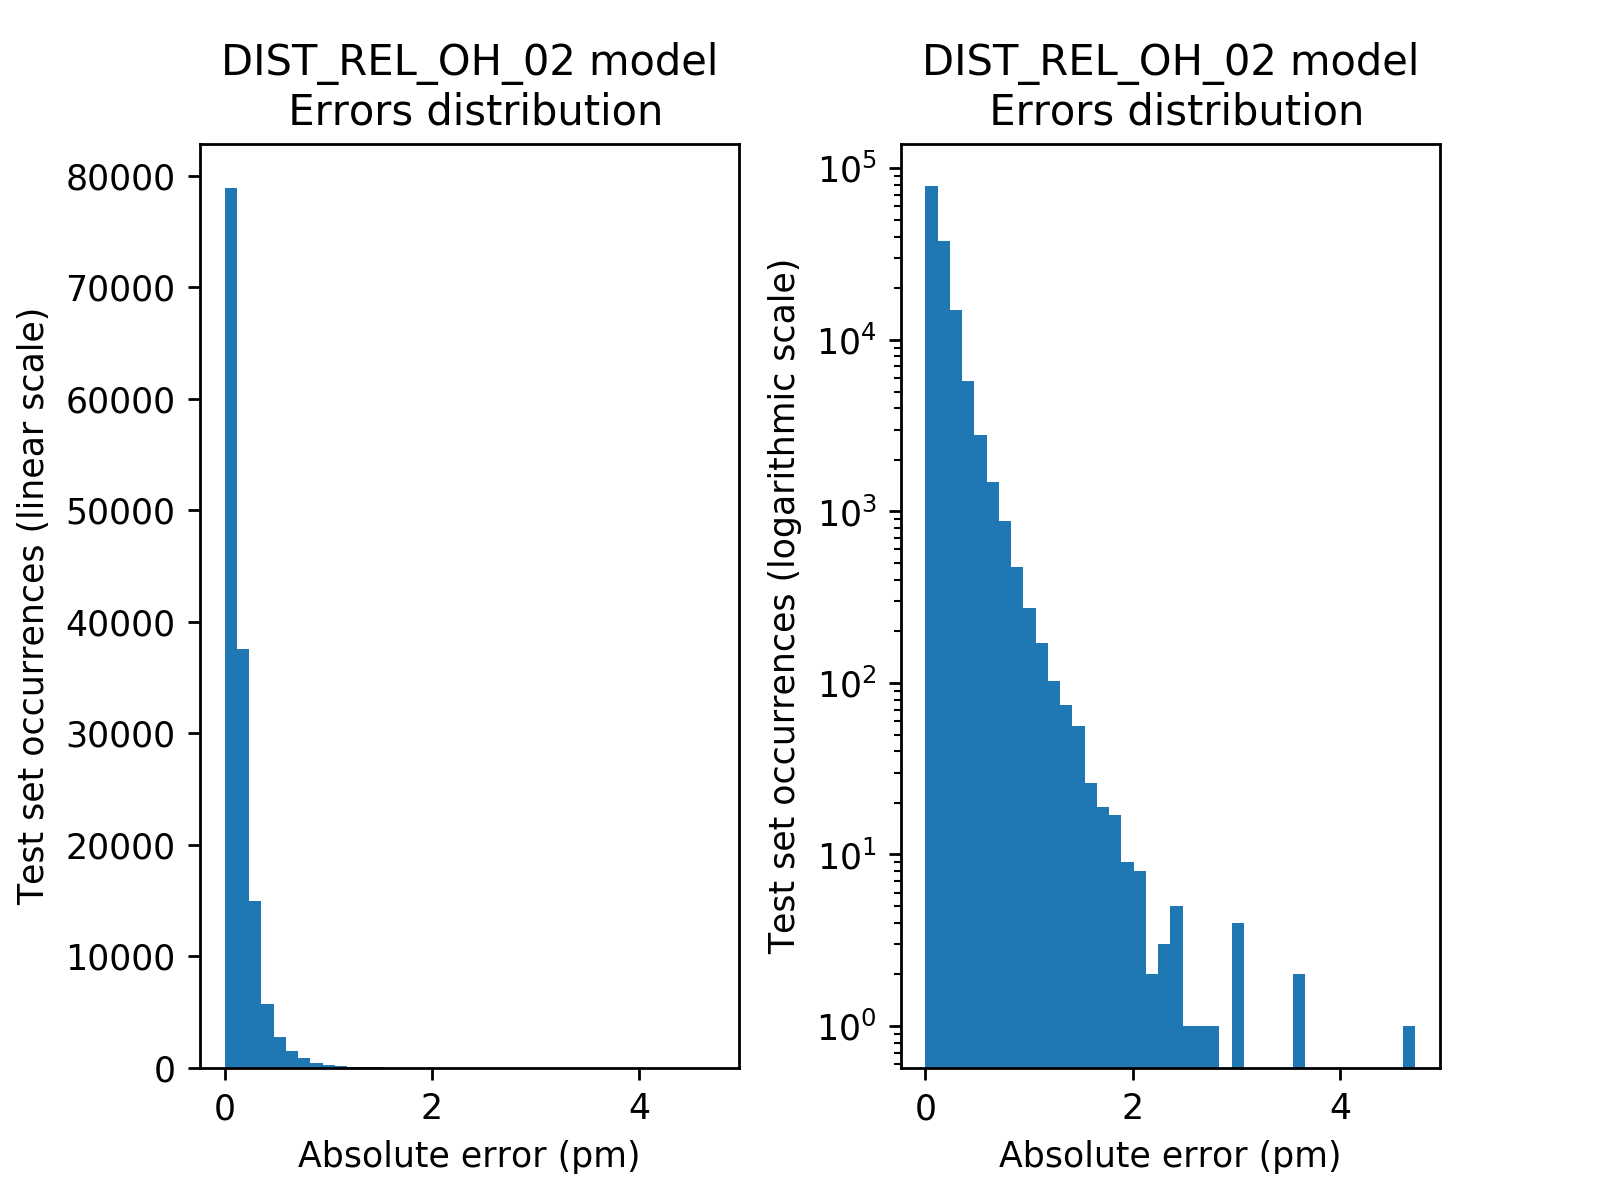
\includegraphics[scale=0.75]{../figures/DIST_REL_OH_02/DIST_REL_OH_02_distrib_rmse_val.png}	
	
	\caption{Distribution des erreurs du modèle \emph{DIST\_REL\_OH\_02}. Modèle s'entraînant sur une \textbf{grande quantité d'exemples} et prédisant les longueurs de liaisons \textbf{oxygène-hydrogène}, à partir de données d'entrées sur lesquelles \textbf{aucune fonction} n'a été appliquée aux distances, \textbf{avec restriction} au voisinage le plus proche.}
\end{figure}
\begin{figure}[!h]
	\centering
	
	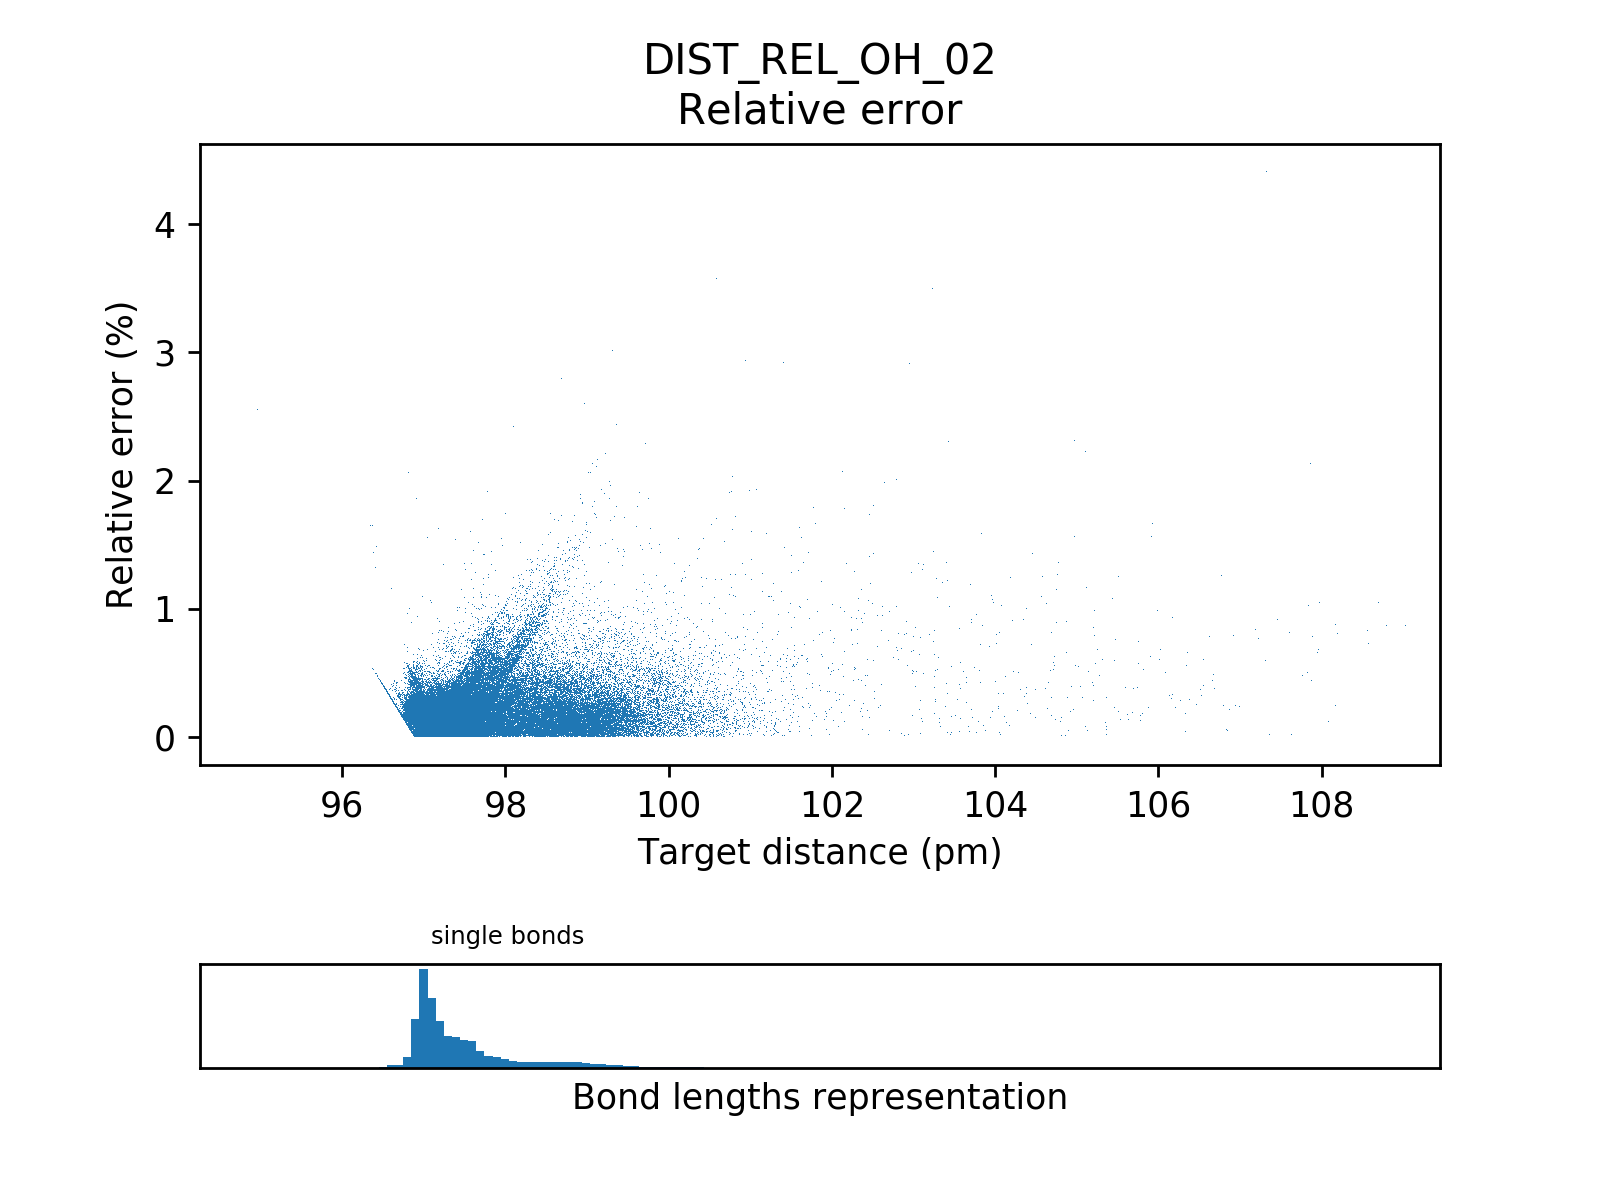
\includegraphics[scale=0.75]{../figures/DIST_REL_OH_02/DIST_REL_OH_02_distrib_rmse_dist.png}	
	
	\caption{Erreur en fonction des cibles pour le modèle \emph{DIST\_REL\_OH\_02}. Modèle s'entraînant sur une \textbf{grande quantité d'exemples} et prédisant les longueurs de liaisons \textbf{oxygène-hydrogène}, à partir de données d'entrées sur lesquelles \textbf{aucune fonction} n'a été appliquée aux distances, \textbf{avec restriction} au voisinage le plus proche.}
	\end{figure}

\begin{figure}[!h]
	\centering
	
	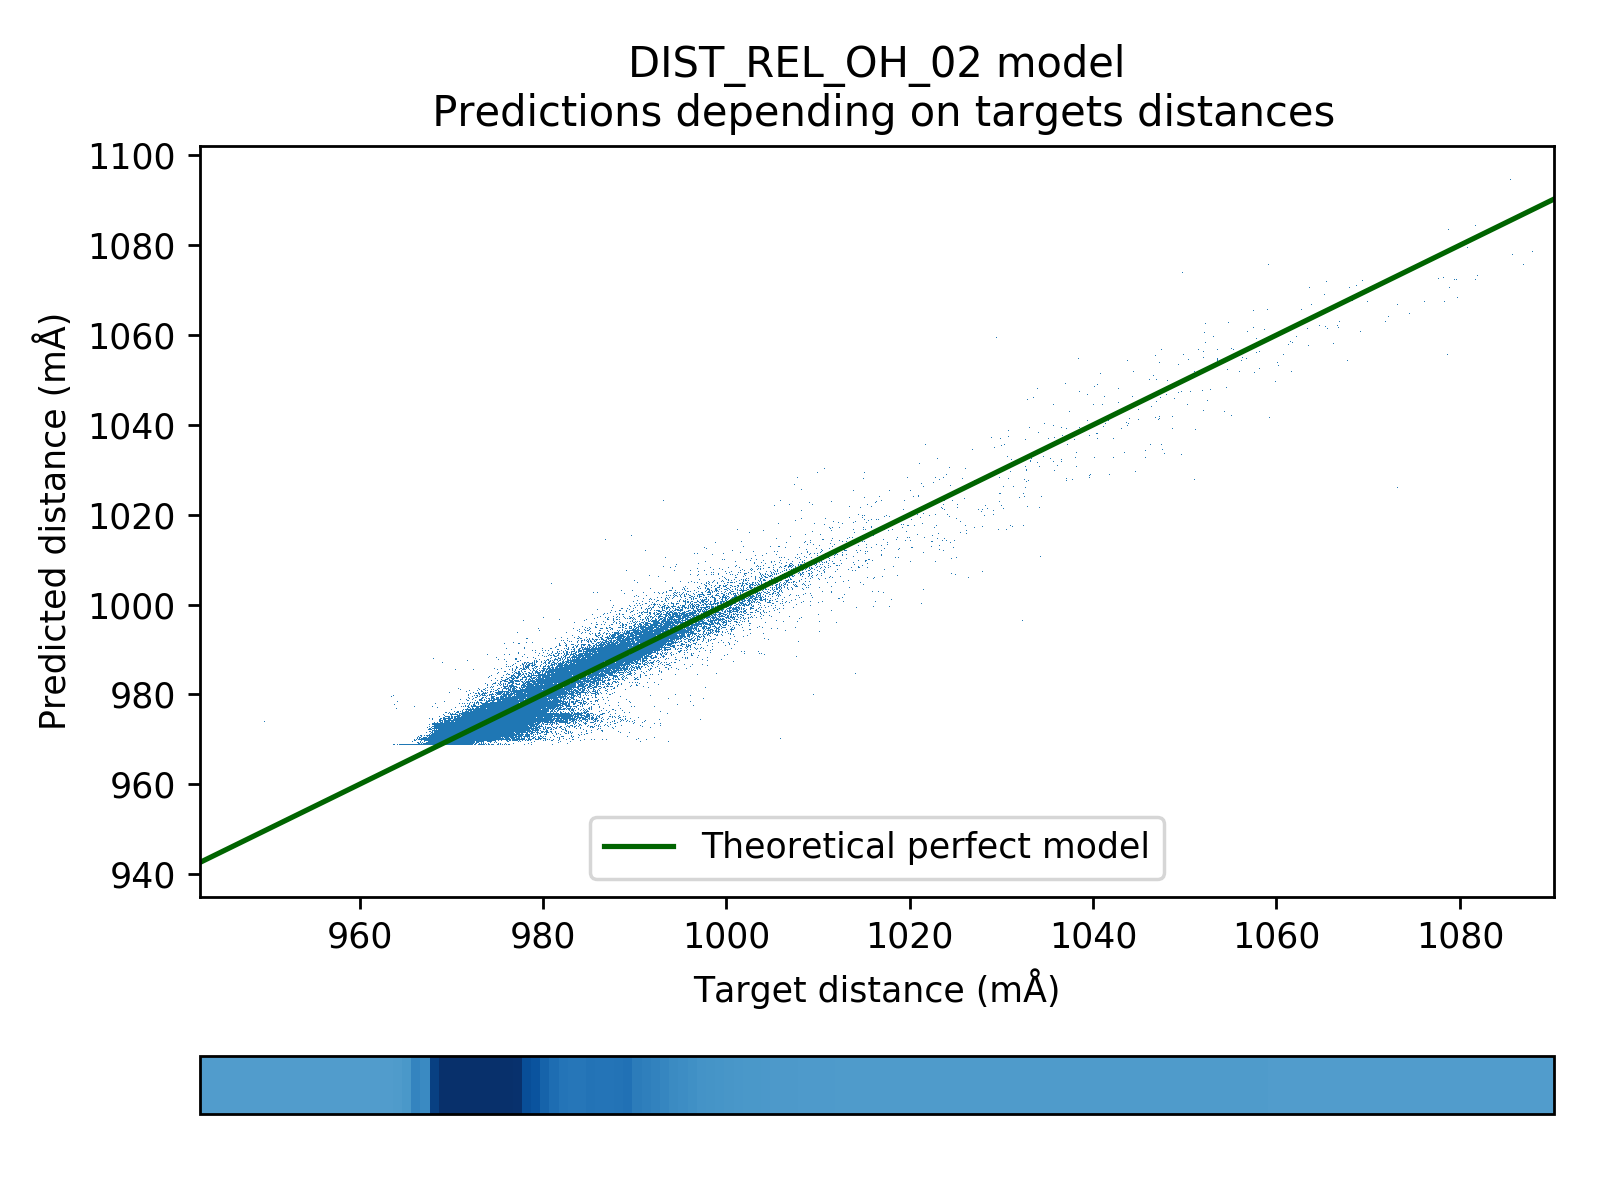
\includegraphics[scale=0.75]{../figures/DIST_REL_OH_02/DIST_REL_OH_02_preds_targets.png}	
	
	\caption{Prédictions en fonction des cibles pour le modèle \emph{DIST\_REL\_OH\_02}. Modèle s'entraînant sur une \textbf{grande quantité d'exemples} et prédisant les longueurs de liaisons \textbf{oxygène-hydrogène}, à partir de données d'entrées sur lesquelles \textbf{aucune fonction} n'a été appliquée aux distances, \textbf{avec restriction} au voisinage le plus proche.}
	
\end{figure}
	
	
% DIST REL CH 02

\begin{figure}[!h]
	\centering
	
	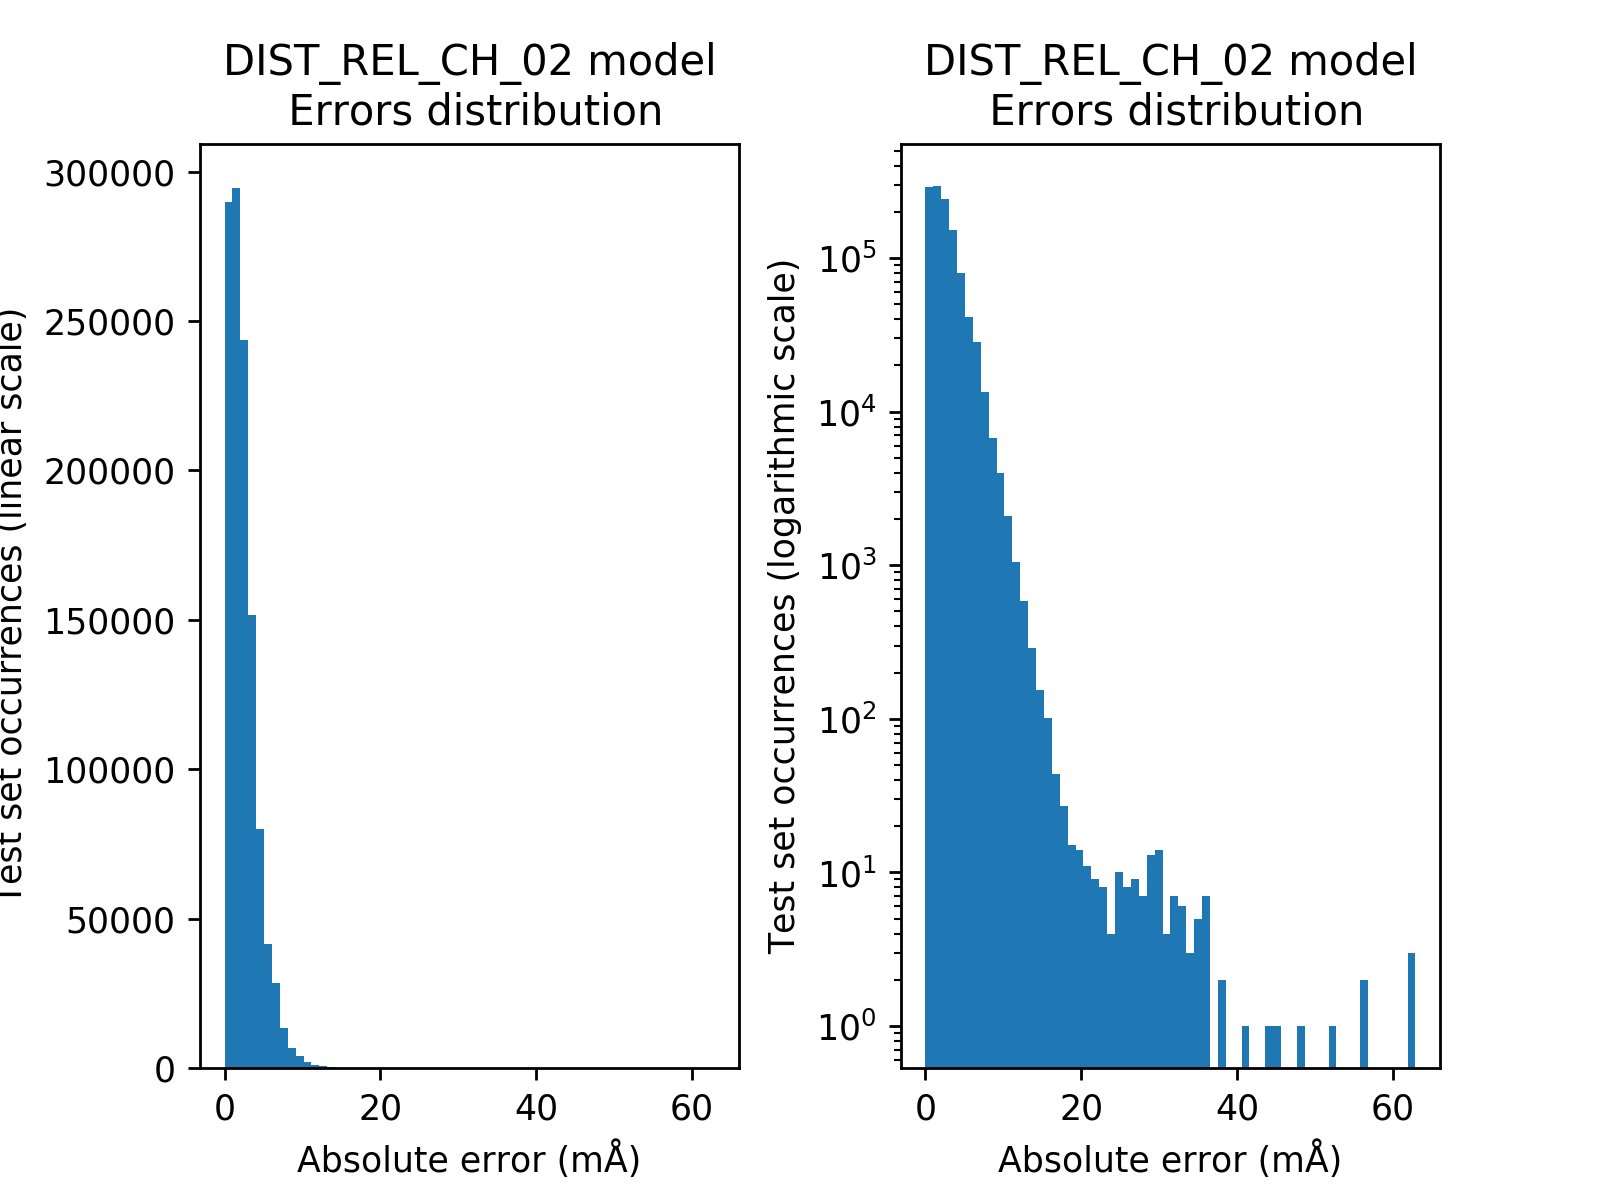
\includegraphics[scale=0.75]{../figures/DIST_REL_CH_02/DIST_REL_CH_02_distrib_rmse_val.png}	
	
	\caption{Distribution des erreurs du modèle \emph{DIST\_REL\_CH\_02}. Modèle s'entraînant sur une \textbf{grande quantité d'exemples} et prédisant les longueurs de liaisons \textbf{carbone-hydrogène}, à partir de données d'entrées sur lesquelles \textbf{aucune fonction} n'a été appliquée aux distances, \textbf{avec restriction} au voisinage le plus proche.}
\end{figure}

\begin{figure}[!h]
	\centering
	
	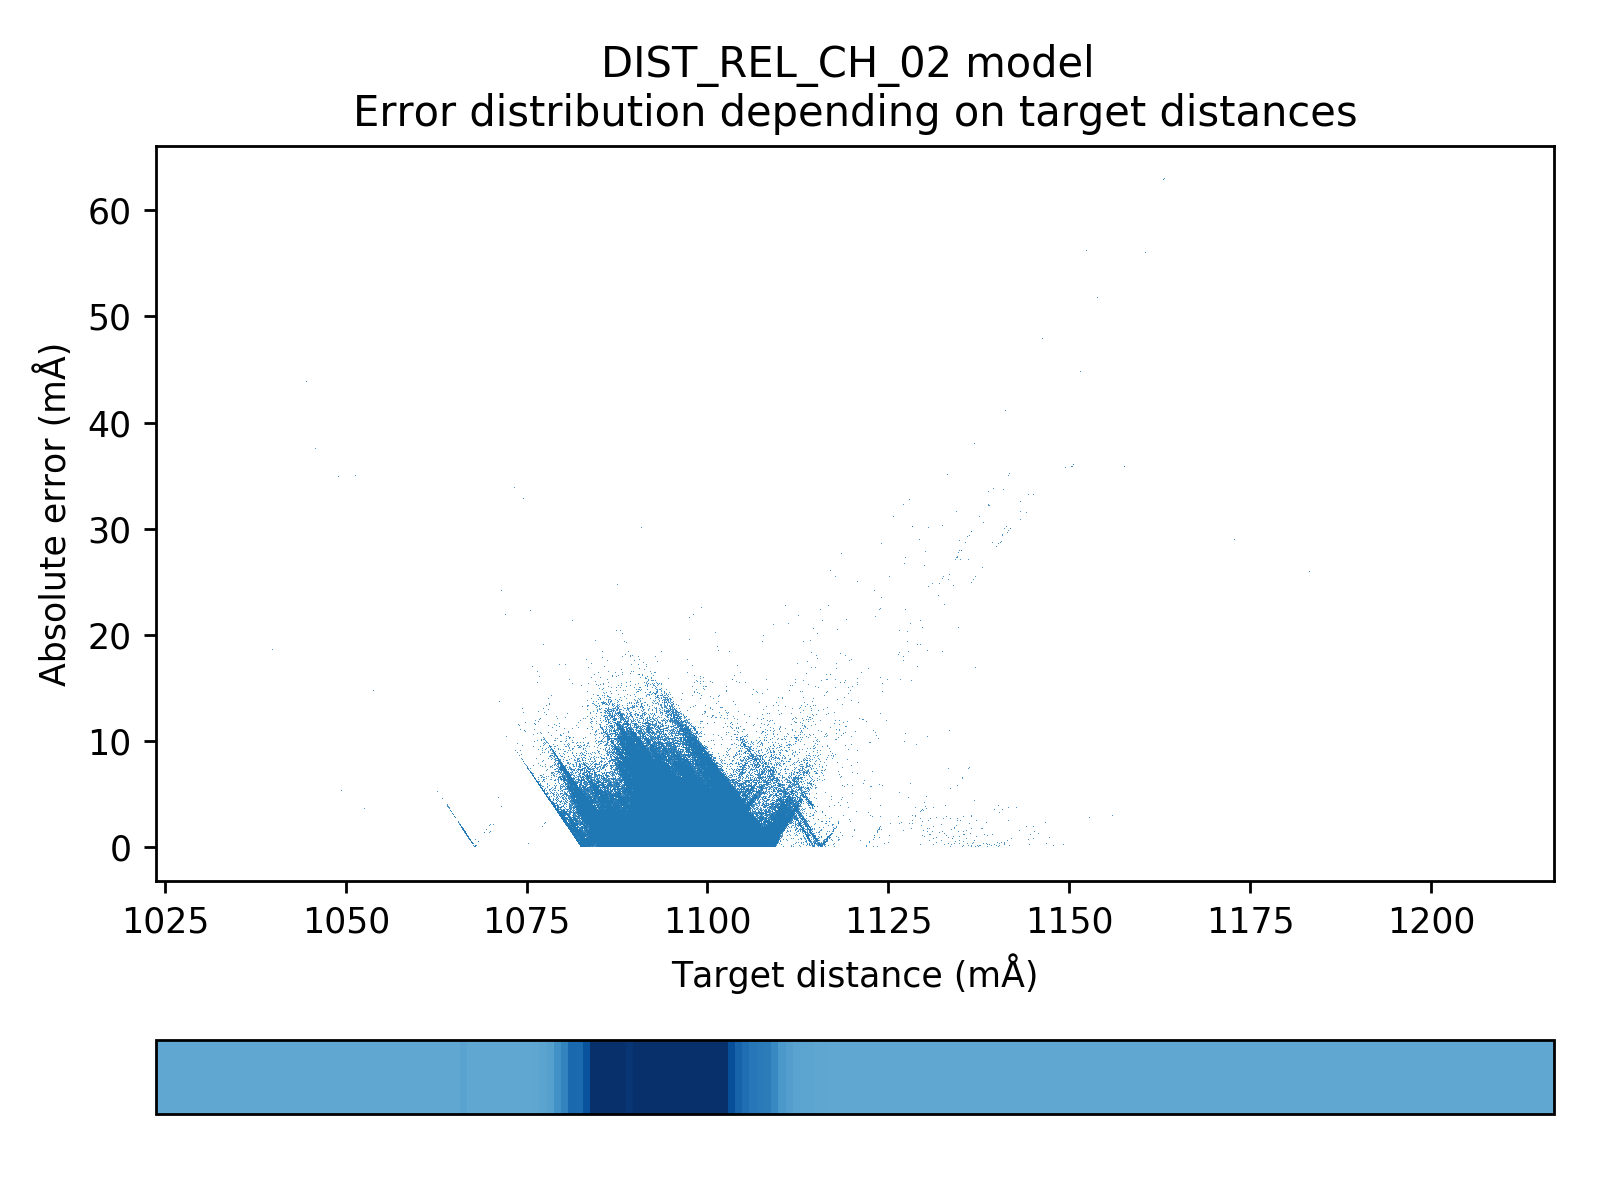
\includegraphics[scale=0.75]{../figures/DIST_REL_CH_02/DIST_REL_CH_02_distrib_rmse_dist.png}	
	
	\caption{Erreur en fonction des cibles pour le modèle \emph{DIST\_REL\_CH\_02}. Modèle s'entraînant sur une \textbf{grande quantité d'exemples} et prédisant les longueurs de liaisons \textbf{carbone-hydrogène}, à partir de données d'entrées sur lesquelles \textbf{aucune fonction} n'a été appliquée aux distances, \textbf{avec restriction} au voisinage le plus proche.}
\end{figure}

\begin{figure}[!h]
	\centering
	
	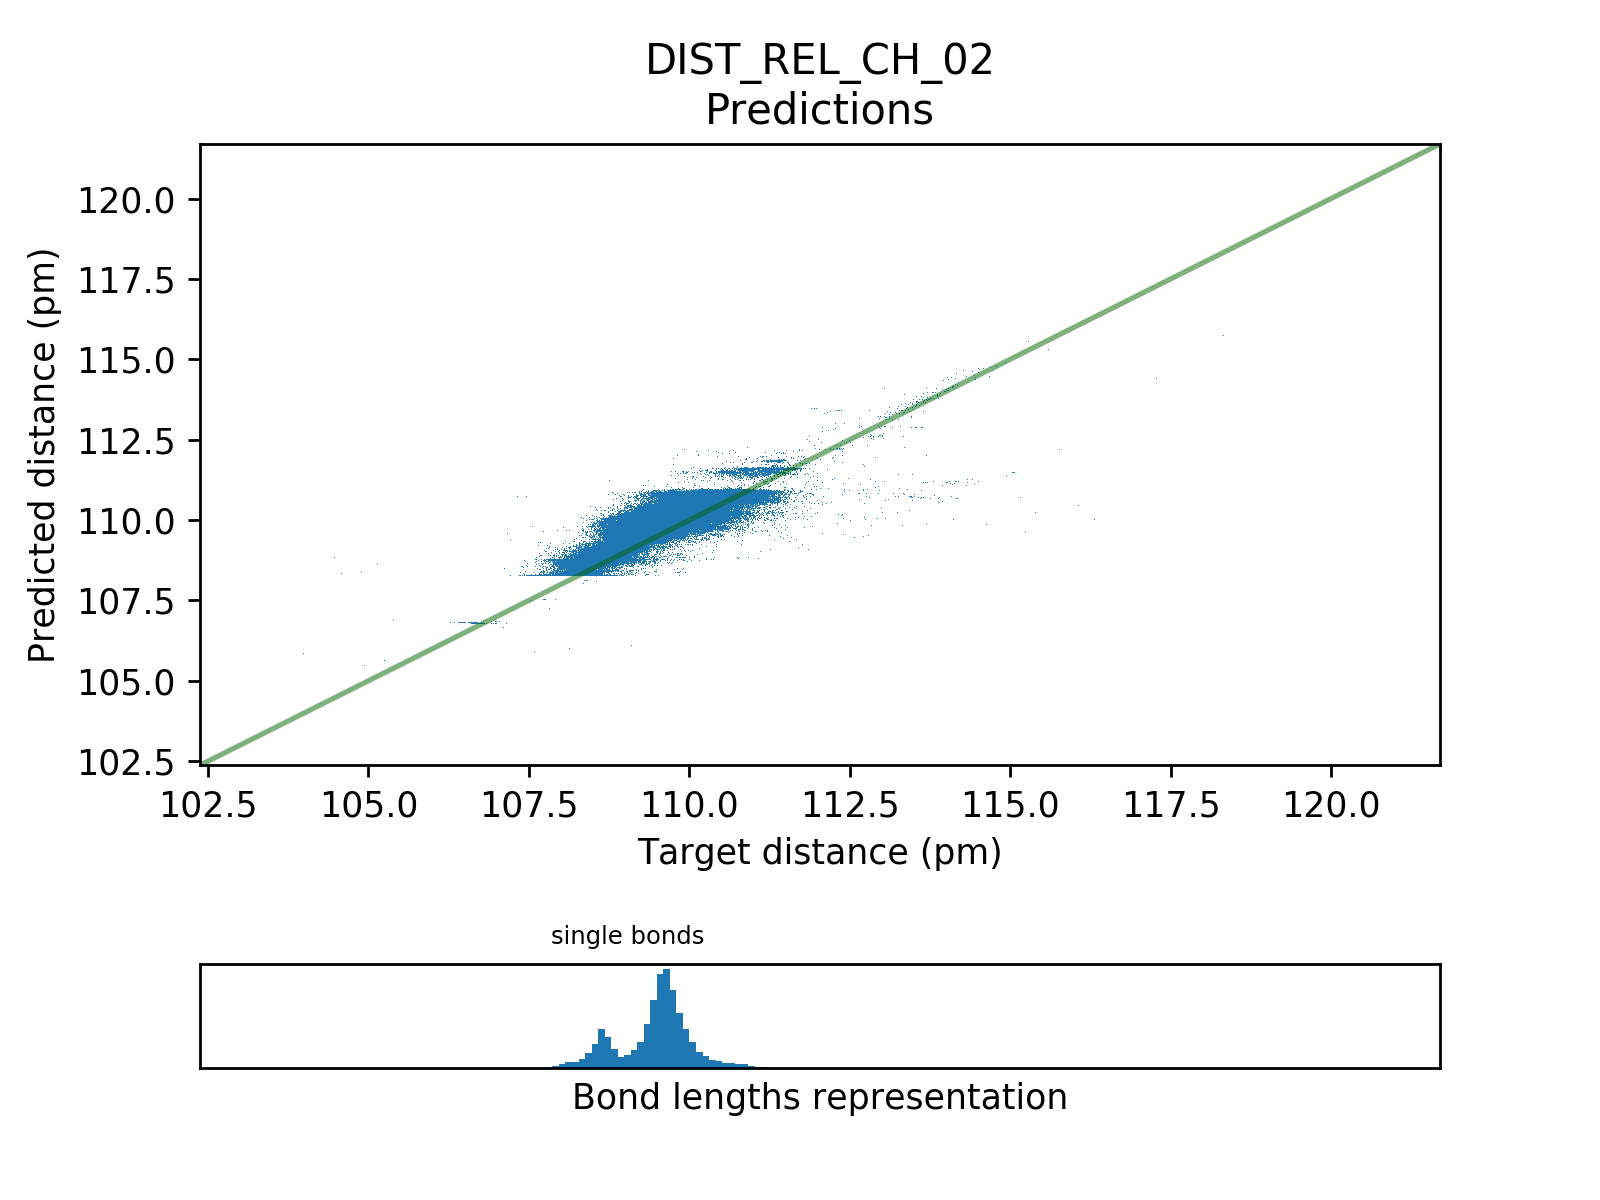
\includegraphics[scale=0.75]{../figures/DIST_REL_CH_02/DIST_REL_CH_02_preds_targets.png}	
	
	\caption{Prédictions en fonction des cibles pour le modèle \emph{DIST\_REL\_OH\_02}. Modèle s'entraînant sur une \textbf{grande quantité d'exemples} et prédisant les longueurs de liaisons \textbf{carbone-hydrogène}, à partir de données d'entrées sur lesquelles \textbf{aucune fonction} n'a été appliquée aux distances, \textbf{avec restriction} au voisinage le plus proche.}
	
\end{figure}


% DIST REL CC 03

\begin{figure}[!h]
	\centering
	
	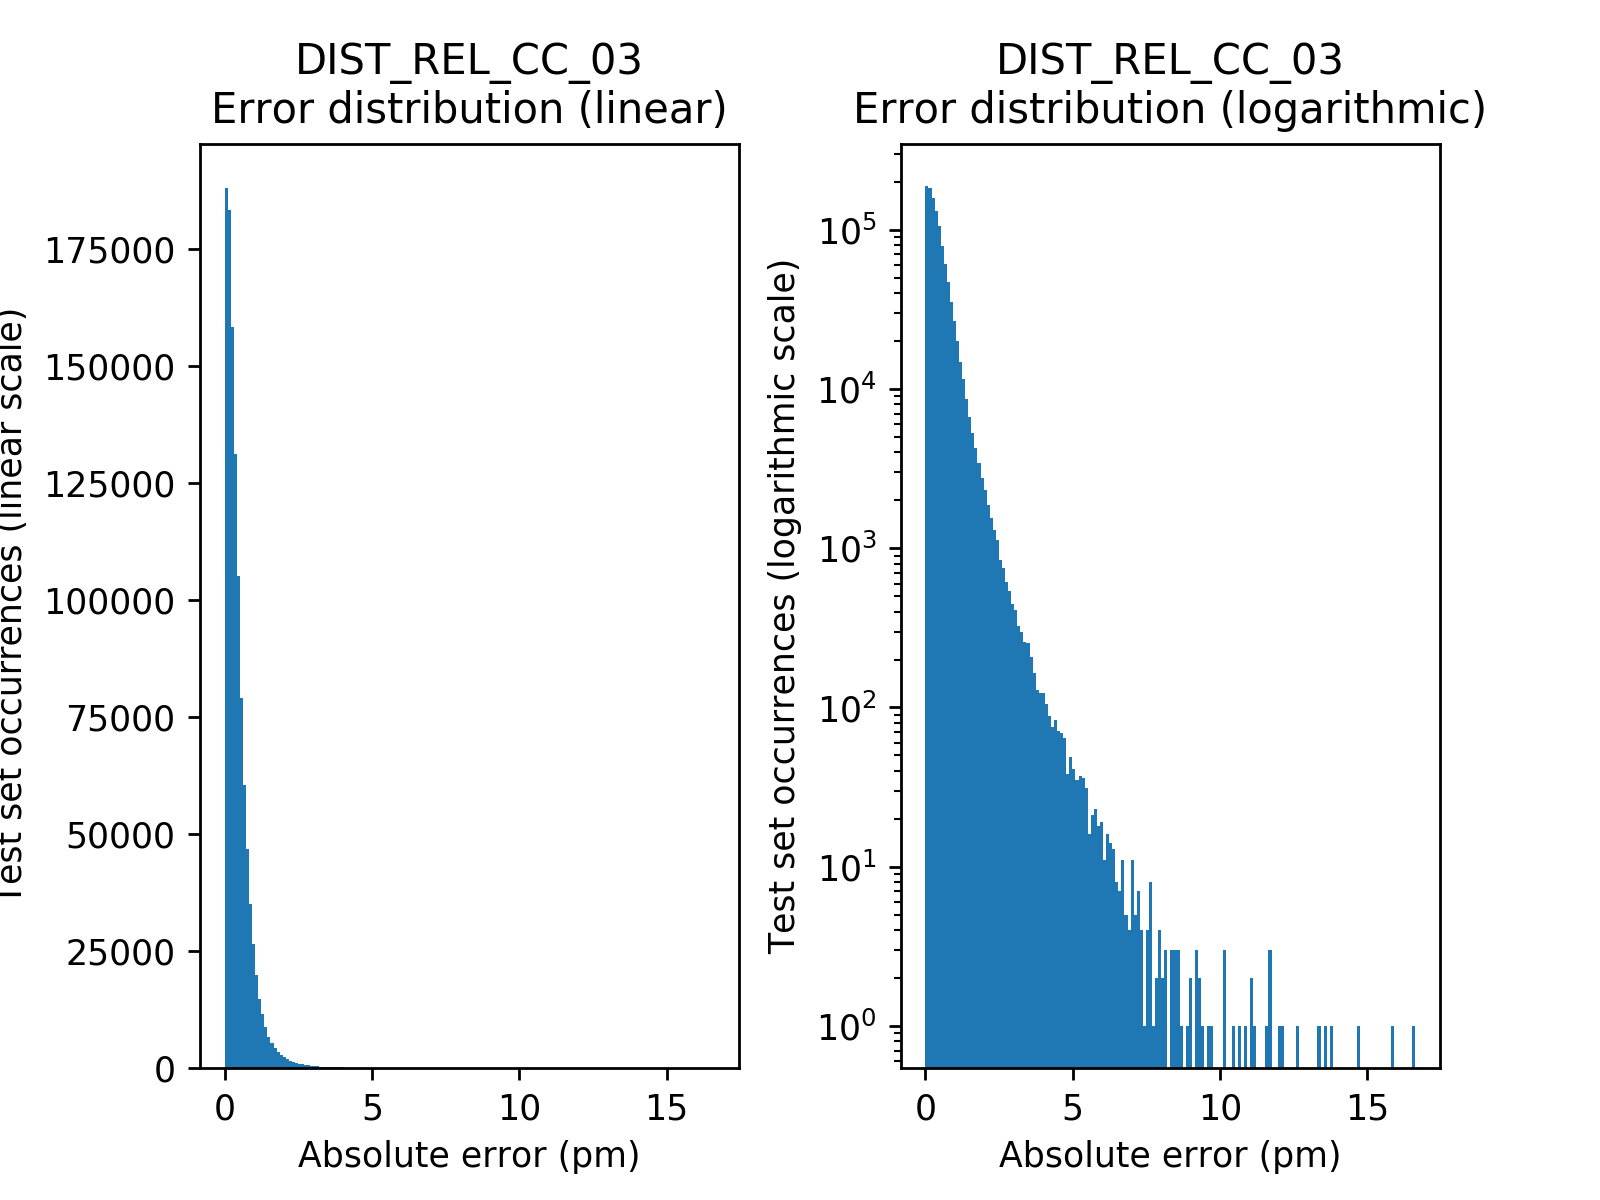
\includegraphics[scale=0.75]{../figures/DIST_REL_CC_03/DIST_REL_CC_03_distrib_rmse_val.png}	
	
	\caption{Distribution des erreurs du modèle \emph{DIST\_REL\_CC\_03}. Modèle s'entraînant sur une \textbf{grande quantité d'exemples} et prédisant les longueurs de liaisons \textbf{carbone-carbone}, à partir de données d'entrées sur lesquelles la \textbf{fonction inverse du carré} a été appliquée aux distances, \textbf{avec restriction} au voisinage le plus proche.}
\end{figure}

\begin{figure}[!h]
	\centering
	
	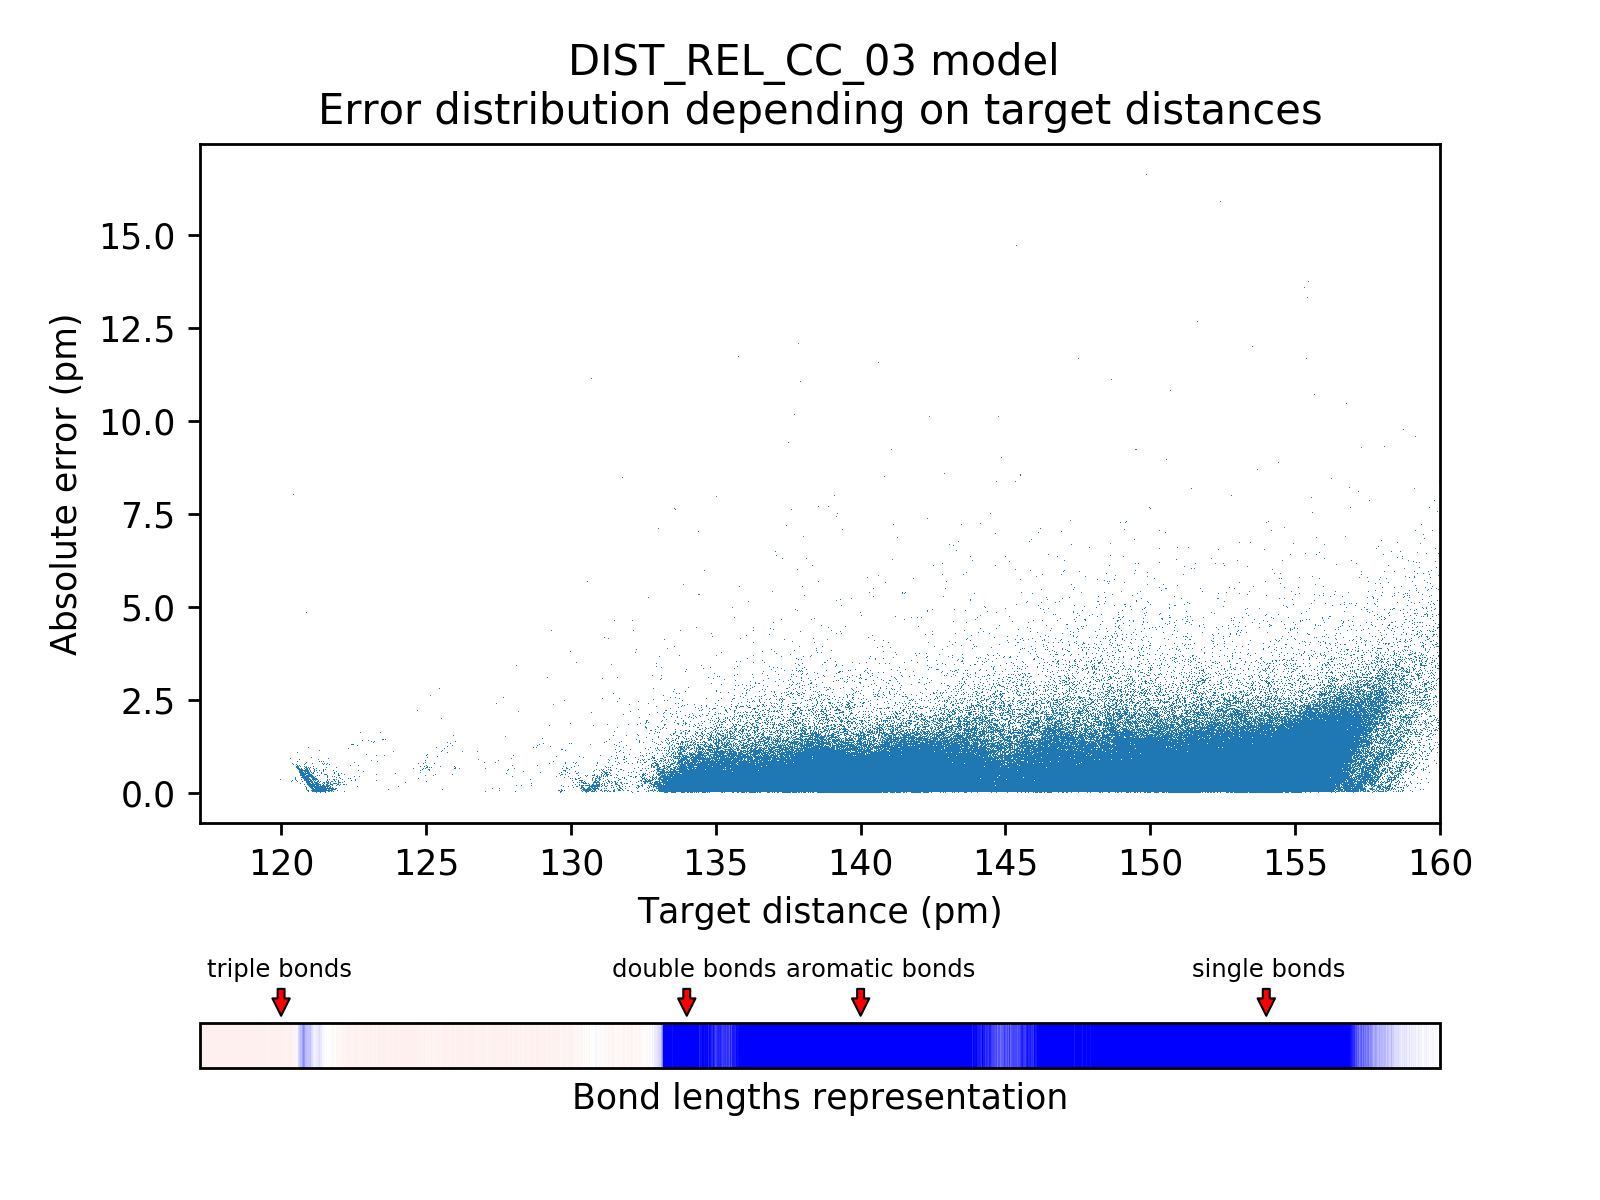
\includegraphics[scale=0.75]{../figures/DIST_REL_CC_03/DIST_REL_CC_03_distrib_rmse_dist.png}	
	
	\caption{Erreur en fonction des cibles pour le modèle \emph{DIST\_REL\_CC\_03}. Modèle s'entraînant sur une \textbf{grande quantité d'exemples} et prédisant les longueurs de liaisons \textbf{carbone-carbone}, à partir de données d'entrées sur lesquelles la \textbf{fonction inverse du carré} a été appliquée aux distances, \textbf{avec restriction} au voisinage le plus proche.}
\end{figure}

\begin{figure}[!h]
	\centering
	
	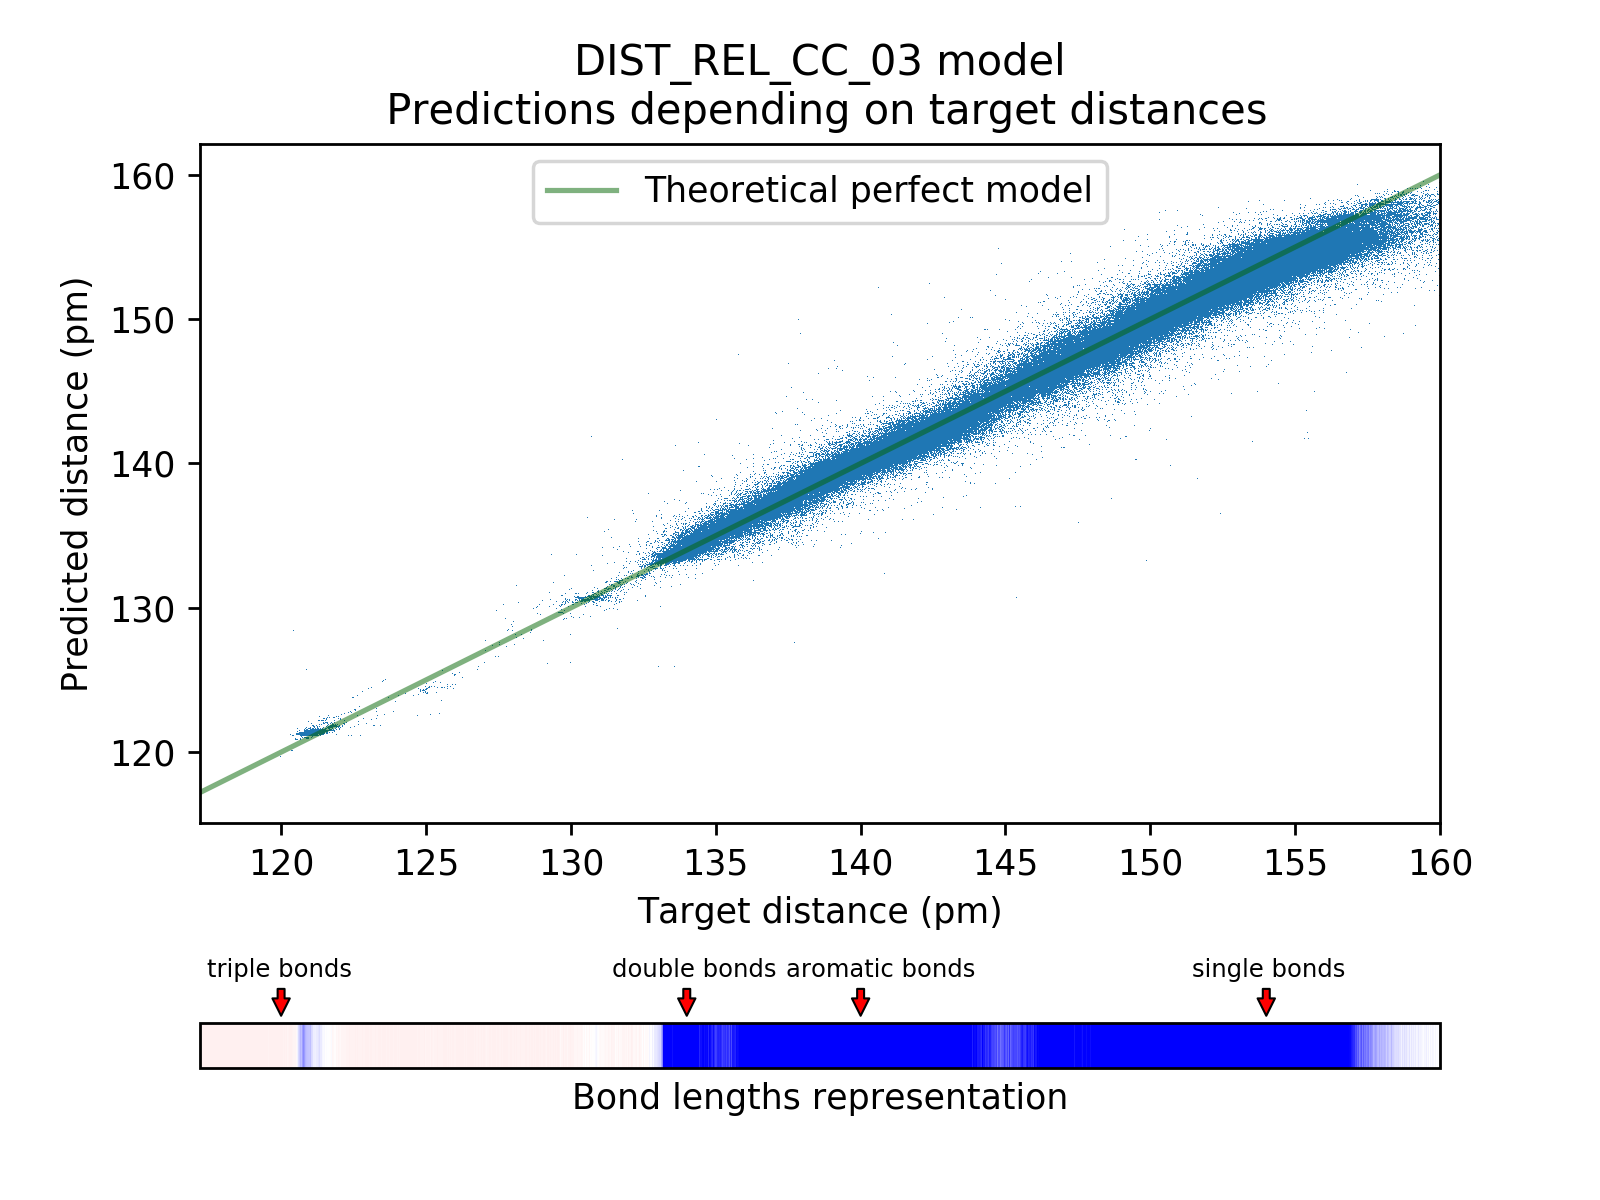
\includegraphics[scale=0.75]{../figures/DIST_REL_CC_03/DIST_REL_CC_03_preds_targets.png}	
	
	\caption{Prédictions en fonction des cibles pour le modèle \emph{DIST\_REL\_CC\_03}. Modèle s'entraînant sur une \textbf{grande quantité d'exemples} et prédisant les longueurs de liaisons \textbf{carbone-carbone}, à partir de données d'entrées sur lesquelles la \textbf{fonction inverse du carré} a été appliquée aux distances, \textbf{avec restriction} au voisinage le plus proche.}
	
\end{figure}

% DIST REL CH 03

\begin{figure}[!h]
	\centering
	
	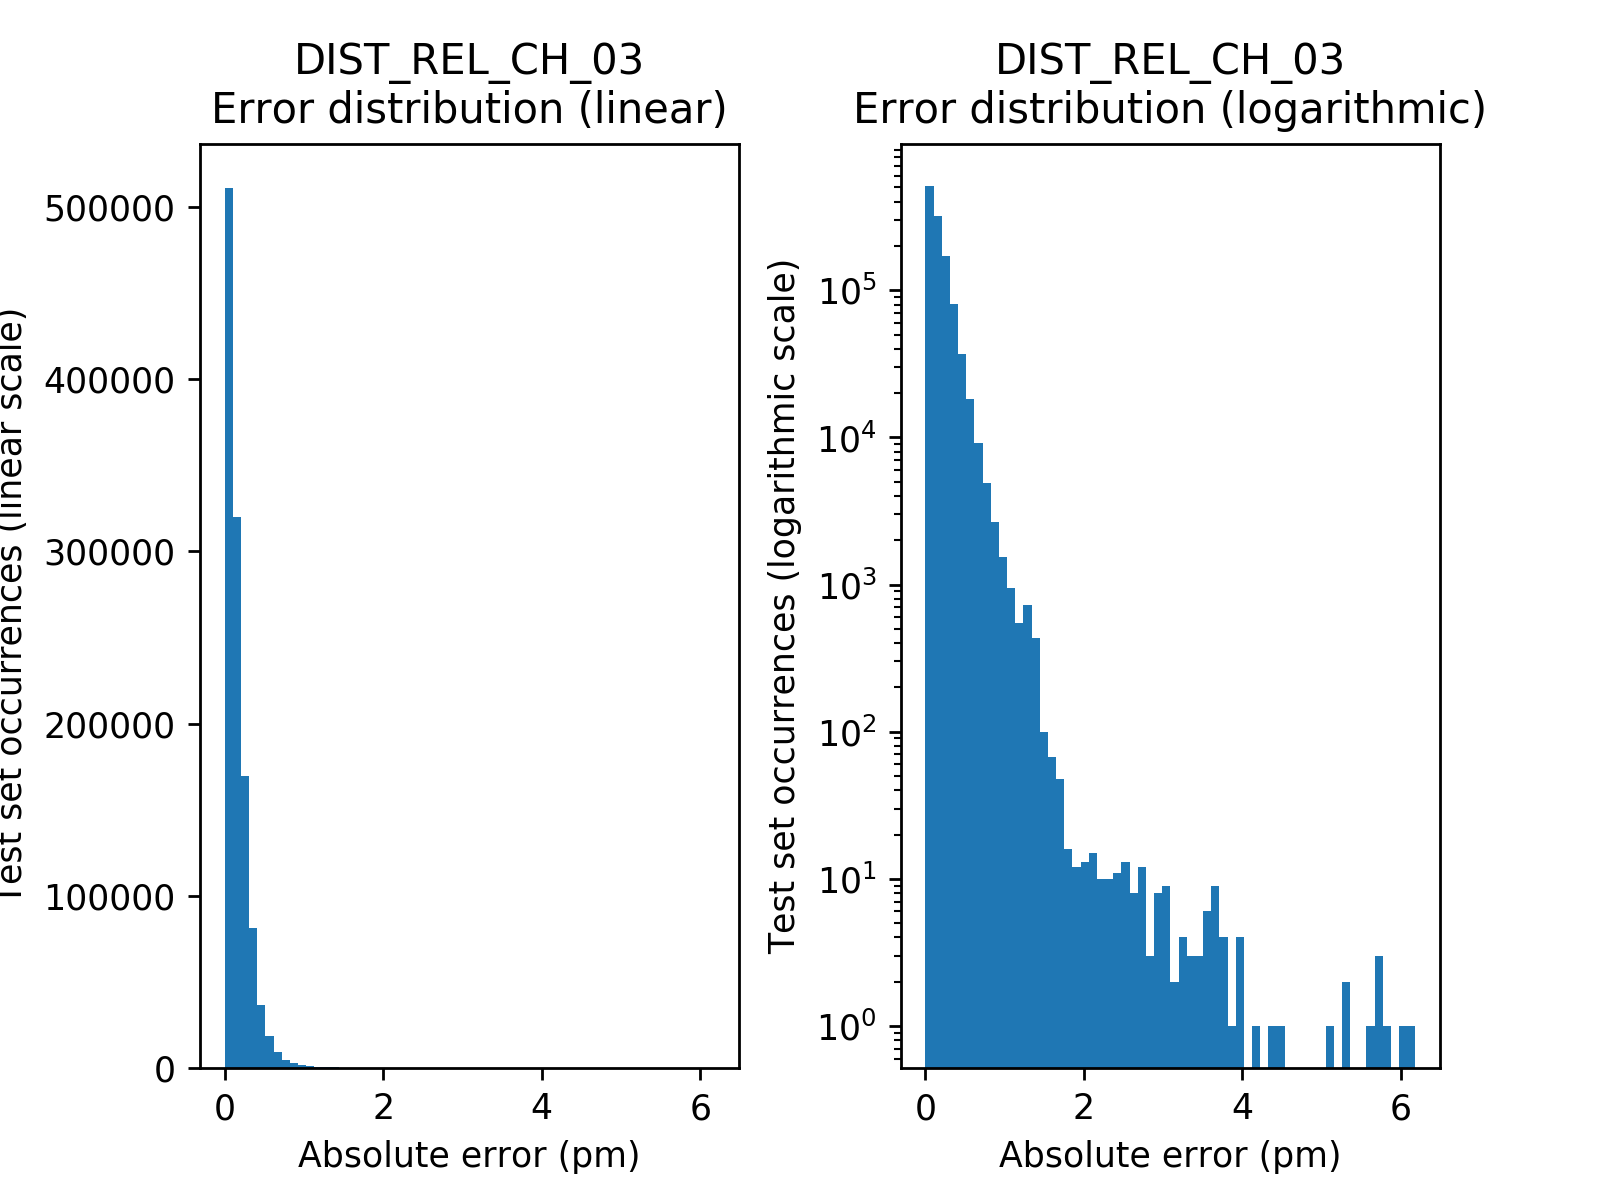
\includegraphics[scale=0.75]{../figures/DIST_REL_CH_03/DIST_REL_CH_03_distrib_rmse_val.png}	
	
	\caption{Distribution des erreurs du modèle \emph{DIST\_REL\_CH\_03}. Modèle s'entraînant sur une \textbf{grande quantité d'exemples} et prédisant les longueurs de liaisons \textbf{carbone-hydrogène}, à partir de données d'entrées sur lesquelles la \textbf{fonction inverse du carré} a été appliquée aux distances, \textbf{avec restriction} au voisinage le plus proche.}
\end{figure}

\begin{figure}[!h]
	\centering
	
	\includegraphics[scale=0.75]{../figures/DIST_REL_CH_03/DIST_REL_CH_03_distrib_rmse_dist.png}	
	
	\caption{Erreur en fonction des cibles pour le modèle \emph{DIST\_REL\_CH\_03}. Modèle s'entraînant sur une \textbf{grande quantité d'exemples} et prédisant les longueurs de liaisons \textbf{carbone-hydrogène}, à partir de données d'entrées sur lesquelles la \textbf{fonction inverse du carré} a été appliquée aux distances, \textbf{avec restriction} au voisinage le plus proche.}
\end{figure}

\begin{figure}[!h]
	\centering
	
	\includegraphics[scale=0.75]{../figures/DIST_REL_CH_03/DIST_REL_CH_03_preds_targets.png}	
	
	\caption{Prédictions en fonction des cibles pour le modèle \emph{DIST\_REL\_CH\_03}. Modèle s'entraînant sur une \textbf{grande quantité d'exemples} et prédisant les longueurs de liaisons \textbf{carbone-hydrogène}, à partir de données d'entrées sur lesquelles la \textbf{fonction inverse du carré} a été appliquée aux distances, \textbf{avec restriction} au voisinage le plus proche.}
	
\end{figure}

% DIST REL OH 03

\begin{figure}[!h]
	\centering
	
	\includegraphics[scale=0.75]{../figures/DIST_REL_OH_03/DIST_REL_OH_03_distrib_rmse_val.png}	
	
	\caption{Distribution des erreurs du modèle \emph{DIST\_REL\_OH\_03}. Modèle s'entraînant sur une \textbf{grande quantité d'exemples} et prédisant les longueurs de liaisons \textbf{oxygène-hydrogène}, à partir de données d'entrées sur lesquelles la \textbf{fonction inverse du carré} a été appliquée aux distances, \textbf{avec restriction} au voisinage le plus proche.}
\end{figure}

\begin{figure}[!h]
	\centering
	
	\includegraphics[scale=0.75]{../figures/DIST_REL_OH_03/DIST_REL_OH_03_distrib_rmse_dist.png}	
	
	\caption{Erreur en fonction des cibles pour le modèle \emph{DIST\_REL\_OH\_03}. Modèle s'entraînant sur une \textbf{grande quantité d'exemples} et prédisant les longueurs de liaisons \textbf{oxygène-hydrogène}, à partir de données d'entrées sur lesquelles la \textbf{fonction inverse du carré} a été appliquée aux distances, \textbf{avec restriction} au voisinage le plus proche.}
\end{figure}

\begin{figure}[!h]
	\centering
	
	\includegraphics[scale=0.75]{../figures/DIST_REL_OH_03/DIST_REL_OH_03_preds_targets.png}	
	
	\caption{Prédictions en fonction des cibles pour le modèle \emph{DIST\_REL\_OH\_03}. Modèle s'entraînant sur une \textbf{grande quantité d'exemples} et prédisant les longueurs de liaisons \textbf{oxygène-hydrogène}, à partir de données d'entrées sur lesquelles la \textbf{fonction inverse du carré} a été appliquée aux distances, \textbf{avec restriction} au voisinage le plus proche.}
	
\end{figure}


% DIST REL CC 04

\begin{figure}[!h]
	\centering
	
	\includegraphics[scale=0.75]{../figures/DIST_REL_CC_04/DIST_REL_CC_04_distrib_rmse_val.png}	
	
	\caption{Distribution des erreurs du modèle \emph{DIST\_REL\_CC\_04}. Modèle s'entraînant sur une \textbf{grande quantité d'exemples} et prédisant les longueurs de liaisons \textbf{carbone-carbone}, à partir de données d'entrées sur lesquelles la \textbf{fonction inverse} a été appliquée aux distances, \textbf{avec restriction} au voisinage le plus proche.}
\end{figure}

\begin{figure}[!h]
	\centering
	
	\includegraphics[scale=0.75]{../figures/DIST_REL_CC_04/DIST_REL_CC_04_distrib_rmse_dist.png}	
	
	\caption{Erreur en fonction des cibles pour le modèle \emph{DIST\_REL\_CC\_04}. Modèle s'entraînant sur une \textbf{grande quantité d'exemples} et prédisant les longueurs de liaisons \textbf{carbone-carbone}, à partir de données d'entrées sur lesquelles la \textbf{fonction inverse} a été appliquée aux distances, \textbf{avec restriction} au voisinage le plus proche.}
\end{figure}

\begin{figure}[!h]
	\centering
	
	\includegraphics[scale=0.75]{../figures/DIST_REL_CC_04/DIST_REL_CC_04_preds_targets.png}	
	
	\caption{Prédictions en fonction des cibles pour le modèle \emph{DIST\_REL\_CC\_04}. Modèle s'entraînant sur une \textbf{grande quantité d'exemples} et prédisant les longueurs de liaisons \textbf{carbone-carbone}, à partir de données d'entrées sur lesquelles la \textbf{fonction inverse} a été appliquée aux distances, \textbf{avec restriction} au voisinage le plus proche.}
	
\end{figure}

% DIST REL CH 04

\begin{figure}[!h]
	\centering
	
	\includegraphics[scale=0.75]{../figures/DIST_REL_CH_04/DIST_REL_CH_04_distrib_rmse_val.png}	
	
	\caption{Distribution des erreurs du modèle \emph{DIST\_REL\_CH\_04}. Modèle s'entraînant sur une \textbf{grande quantité d'exemples} et prédisant les longueurs de liaisons \textbf{carbone-hydrogene}, à partir de données d'entrées sur lesquelles la \textbf{fonction inverse} a été appliquée aux distances, \textbf{avec restriction} au voisinage le plus proche.}
\end{figure}

\begin{figure}[!h]
	\centering
	
	\includegraphics[scale=0.75]{../figures/DIST_REL_CH_04/DIST_REL_CH_04_distrib_rmse_dist.png}	
	
	\caption{Erreur en fonction des cibles pour le modèle \emph{DIST\_REL\_CH\_04}. Modèle s'entraînant sur une \textbf{grande quantité d'exemples} et prédisant les longueurs de liaisons \textbf{carbone-hydrogene}, à partir de données d'entrées sur lesquelles la \textbf{fonction inverse} a été appliquée aux distances, \textbf{avec restriction} au voisinage le plus proche.}
\end{figure}

\begin{figure}[!h]
	\centering
	
	\includegraphics[scale=0.75]{../figures/DIST_REL_CH_04/DIST_REL_CH_04_preds_targets.png}	
	
	\caption{Prédictions en fonction des cibles pour le modèle \emph{DIST\_REL\_CH\_04}. Modèle s'entraînant sur une \textbf{grande quantité d'exemples} et prédisant les longueurs de liaisons \textbf{carbone-hydrogene}, à partir de données d'entrées sur lesquelles la \textbf{fonction inverse} a été appliquée aux distances, \textbf{avec restriction} au voisinage le plus proche.}
	
\end{figure}

% DIST REL OH 04

\begin{figure}[!h]
	\centering
	
	\includegraphics[scale=0.75]{../figures/DIST_REL_OH_04/DIST_REL_OH_04_distrib_rmse_val.png}	
	
	\caption{Distribution des erreurs du modèle \emph{DIST\_REL\_OH\_04}. Modèle s'entraînant sur une \textbf{grande quantité d'exemples} et prédisant les longueurs de liaisons \textbf{oxygène-hydrogene}, à partir de données d'entrées sur lesquelles la \textbf{fonction inverse} a été appliquée aux distances, \textbf{avec restriction} au voisinage le plus proche.}
\end{figure}

\begin{figure}[!h]
	\centering
	
	\includegraphics[scale=0.75]{../figures/DIST_REL_OH_04/DIST_REL_OH_04_distrib_rmse_dist.png}	
	
	\caption{Erreur en fonction des cibles pour le modèle \emph{DIST\_REL\_OH\_04}. Modèle s'entraînant sur une \textbf{grande quantité d'exemples} et prédisant les longueurs de liaisons \textbf{oxygène-hydrogene}, à partir de données d'entrées sur lesquelles la \textbf{fonction inverse} a été appliquée aux distances, \textbf{avec restriction} au voisinage le plus proche.}
\end{figure}

\begin{figure}[!h]
	\centering
	
	\includegraphics[scale=0.75]{../figures/DIST_REL_OH_04/DIST_REL_OH_04_preds_targets.png}	
	
	\caption{Prédictions en fonction des cibles pour le modèle \emph{DIST\_REL\_OH\_04}. Modèle s'entraînant sur une \textbf{grande quantité d'exemples} et prédisant les longueurs de liaisons \textbf{oxygène-hydrogene}, à partir de données d'entrées sur lesquelles la \textbf{fonction inverse} a été appliquée aux distances, \textbf{avec restriction} au voisinage le plus proche.}
	
\end{figure}

\chapter{Résultats de la recherche par quadrillage du modèle KRR}

\label{annexes_krr_quadri}

\begin{verbatim}

0.935 (+/-0.007) for {'coef0': 1, 'kernel': 'linear', 'degree': 1, 'gamma': None, 'alpha': 0.1}
0.726 (+/-0.292) for {'coef0': 1, 'kernel': 'linear', 'degree': 1, 'gamma': None, 'alpha': 0.01}
0.615 (+/-0.495) for {'coef0': 1, 'kernel': 'linear', 'degree': 1, 'gamma': None, 'alpha': 0.001}
0.935 (+/-0.011) for {'coef0': 1, 'kernel': 'poly', 'degree': 2, 'gamma': None, 'alpha': 0.1}
0.817 (+/-0.285) for {'coef0': 1, 'kernel': 'poly', 'degree': 6, 'gamma': None, 'alpha': 0.1}
0.934 (+/-0.012) for {'coef0': 0.5, 'kernel': 'poly', 'degree': 2, 'gamma': None, 'alpha': 0.1}
0.586 (+/-0.772) for {'coef0': 0.5, 'kernel': 'poly', 'degree': 6, 'gamma': None, 'alpha': 0.1}
0.937 (+/-0.010) for {'coef0': 2, 'kernel': 'poly', 'degree': 2, 'gamma': None, 'alpha': 0.1}
0.899 (+/-0.124) for {'coef0': 2, 'kernel': 'poly', 'degree': 6, 'gamma': None, 'alpha': 0.1}
0.951 (+/-0.006) for {'coef0': 1, 'kernel': 'poly', 'degree': 2, 'gamma': None, 'alpha': 0.01}
0.760 (+/-0.384) for {'coef0': 1, 'kernel': 'poly', 'degree': 6, 'gamma': None, 'alpha': 0.01}
0.950 (+/-0.007) for {'coef0': 0.5, 'kernel': 'poly', 'degree': 2, 'gamma': None, 'alpha': 0.01}
0.703 (+/-0.312) for {'coef0': 0.5, 'kernel': 'poly', 'degree': 6, 'gamma': None, 'alpha': 0.01}
0.951 (+/-0.006) for {'coef0': 2, 'kernel': 'poly', 'degree': 2, 'gamma': None, 'alpha': 0.01}
0.909 (+/-0.107) for {'coef0': 2, 'kernel': 'poly', 'degree': 6, 'gamma': None, 'alpha': 0.01}
0.917 (+/-0.049) for {'coef0': 1, 'kernel': 'poly', 'degree': 2, 'gamma': None, 'alpha': 0.001}
0.742 (+/-0.394) for {'coef0': 1, 'kernel': 'poly', 'degree': 6, 'gamma': None, 'alpha': 0.001}
0.942 (+/-0.004) for {'coef0': 0.5, 'kernel': 'poly', 'degree': 2, 'gamma': None, 'alpha': 0.001}
0.699 (+/-0.330) for {'coef0': 0.5, 'kernel': 'poly', 'degree': 6, 'gamma': None, 'alpha': 0.001}
0.935 (+/-0.012) for {'coef0': 2, 'kernel': 'poly', 'degree': 2, 'gamma': None, 'alpha': 0.001}
0.895 (+/-0.146) for {'coef0': 2, 'kernel': 'poly', 'degree': 6, 'gamma': None, 'alpha': 0.001}
Best score: 0.951
Best parameters set:
{'kernel_params': None, 'kernel': 'poly', 'degree': 2, 'gamma': None, 'alpha': 0.01, 'coef0': 1}
\end{verbatim}


\begin{landscape}

\chapter{Paramètres des modèles \emph{DELTA\_DIST\_+H}}

\label{annexes_param_delta_dist}

\centering

\begin{tabular}{|c|c|c|c|c|c|c|c|c|c|c|c|}
\hline
\begin{minipage}{3.5cm} \vspace{5mm}Modèle\vspace{5mm}\end{minipage} & 
\begin{minipage}{1.3cm}Tailles \\molécules\end{minipage} & 
\begin{minipage}{1.8cm}Repr. géom.\\ entrée\end{minipage} & 
\begin{minipage}{1.8cm}Repr. géom.\\ sortie \end{minipage} & 
\begin{minipage}{1.4cm}Numéros\\ atomiques \end{minipage} & 
\begin{minipage}{1.4cm}Masses\\ atomiques \end{minipage} &
\begin{minipage}{2cm}Distances inter at. fictifs \end{minipage} & 
\begin{minipage}{1.8cm}Fonction de coût \end{minipage} & 
\begin{minipage}{1.65cm}Profondeur \end{minipage} & 
\begin{minipage}{1.2cm}Largeur \end{minipage} & 
\begin{minipage}{1cm}Taille\\ entrée \end{minipage} & 
\begin{minipage}{0.9cm}Bruit \end{minipage} \\  \hline

\begin{minipage}{3.5cm}\vspace{5mm}DELTA\_DIST+H\_01 \vspace{1mm} \end{minipage} &
\begin{minipage}{1.3cm}0 - 200 \end{minipage} &
\begin{minipage}{1.8cm}Matr. dist. pts. fixes \end{minipage} &
\begin{minipage}{1.8cm}Matr. dist. pts. fixes \end{minipage} &
\begin{minipage}{1.4cm}Non \end{minipage} &
\begin{minipage}{1.4cm}Oui \end{minipage} &
\begin{minipage}{2cm} Non \end{minipage} &
\begin{minipage}{1.8cm}RMSE\\ partiel/total \end{minipage}&
\begin{minipage}{1.65cm} 4 \end{minipage}&
\begin{minipage}{1.2cm} 8650 \end{minipage} &
\begin{minipage}{1cm}1000 \end{minipage} &
\begin{minipage}{0.9cm}+/++ \end{minipage} \\  \hline

\begin{minipage}{3.5cm}\vspace{5mm}DELTA\_DIST+H\_02 \vspace{1mm} \end{minipage} &
\begin{minipage}{1.3cm}0 - 200 \end{minipage} &
\begin{minipage}{1.8cm}Matr. dist. pts. fixes \end{minipage} &
\begin{minipage}{1.8cm}Matr. dist. pts. fixes \end{minipage} &
\begin{minipage}{1.4cm}Non \end{minipage} &
\begin{minipage}{1.4cm}Oui \end{minipage} &
\begin{minipage}{2cm} Oui \end{minipage} &
\begin{minipage}{1.8cm}RMSE\\ partiel \end{minipage}&
\begin{minipage}{1.65cm} 4 \end{minipage}&
\begin{minipage}{1.2cm} 8650 \end{minipage} &
\begin{minipage}{1cm}1020 \end{minipage} &
\begin{minipage}{0.9cm}+ \end{minipage} \\  \hline

\begin{minipage}{3.3cm}\vspace{1cm}DELTA\_DIST+H\_03 \vspace{5mm} \end{minipage} &
\begin{minipage}{1.3cm}0 - 200 \end{minipage} &
\begin{minipage}{1.8cm}Matr. dist. pts. fixes + \\ Matr red. dist. inter-at. \end{minipage} &
\begin{minipage}{1.8cm}Matr. dist. pts. fixes \end{minipage} &
\begin{minipage}{1.4cm}Non \end{minipage} &
\begin{minipage}{1.4cm}Oui \end{minipage} &
\begin{minipage}{2cm} Non \end{minipage} &
\begin{minipage}{1.8cm}RMSE\\ partiel \end{minipage}&
\begin{minipage}{1.65cm} 3 \end{minipage}&
\begin{minipage}{1.2cm} 9000 \end{minipage} &
\begin{minipage}{1cm}1800\end{minipage} &
\begin{minipage}{0.9cm}++ \end{minipage} \\  \hline

\begin{minipage}{3.5cm}\vspace{1cm}DELTA\_DIST+H\_04 \vspace{5mm} \end{minipage} &
\begin{minipage}{1.3cm}0 - 200 \end{minipage} &
\begin{minipage}{1.8cm}Matr. dist. pts. fixes + \\ Matr red. dist. inter-at. \end{minipage} &
\begin{minipage}{1.8cm} Matr red. dist. inter-at. \end{minipage} &
\begin{minipage}{1.4cm}Non \end{minipage} &
\begin{minipage}{1.4cm}Oui \end{minipage} &
\begin{minipage}{2cm} Non \end{minipage} &
\begin{minipage}{1.8cm}RMSE\\ partiel \end{minipage}&
\begin{minipage}{1.65cm} 3 \end{minipage}&
\begin{minipage}{1.2cm} 9000 \end{minipage} &
\begin{minipage}{1cm}1800\end{minipage} &
\begin{minipage}{0.9cm}++ \end{minipage} \\  \hline


\begin{minipage}{3.5cm}\vspace{1cm}DELTA\_DIST+H\_05 \vspace{5mm} \end{minipage} &
\begin{minipage}{1.3cm}2 - 60 \end{minipage} &
\begin{minipage}{1.8cm}Matr. dist. pts. fixes \end{minipage} &
\begin{minipage}{1.8cm}Matr. dist. pts. fixes \end{minipage} &
\begin{minipage}{1.4cm}Oui \end{minipage} &
\begin{minipage}{1.4cm}Oui \end{minipage} &
\begin{minipage}{2cm} Non \end{minipage} &
\begin{minipage}{1.8cm}RMSE\\ partiel \end{minipage}&
\begin{minipage}{1.65cm} 3 \end{minipage}&
\begin{minipage}{1.2cm} 360 \end{minipage} &
\begin{minipage}{1cm} 360 \end{minipage} &
\begin{minipage}{0.9cm}++ \end{minipage} \\  \hline


\end{tabular}

\end{landscape}





\end{document}